%\documentclass[11pt,twoside,a4paper,final]{book}
\documentclass[11pt,twoside,a4paper,final]{book}


\bibliographystyle{myelsart-harv}

%\usepackage{afterpage} % To process floats
\usepackage{amsmath} % To be able to use \text
\usepackage{booktabs} % To have better tables
\usepackage[usenames]{color}
\usepackage{fancyhdr} % To control header- and footer layout
\usepackage{graphicx} % To include EPS figures
\usepackage{ifthen} % To use ifthenelse in newcommand
\usepackage[round]{natbib} % To have more versatile citations
%\usepackage{rotating} % For sideways tables
%\usepackage{siunitx} % To have SI units
\usepackage{SIunits}
\usepackage{times} %TrueType times font
\usepackage{topcapt} % For captions above tables

\usepackage[T1]{fontenc} % To use Type 1 instead of Type 3 fonts in PS file
\usepackage{ae,aecompl}

%----------------------------------------------------------------------------------------------------
% Allow more floating material on text pages
%----------------------------------------------------------------------------------------------------

\renewcommand\floatpagefraction{.9}%
\renewcommand\topfraction{.9}%
\renewcommand\bottomfraction{.9}%
\renewcommand\textfraction{.1}%
\setcounter{bottomnumber}{4}%
\setcounter{topnumber}{4}%
\setcounter{totalnumber}{4}%

%----------------------------------------------------------------------------------------------------
% Create really empty pages before new chapters (from Patrick)
%----------------------------------------------------------------------------------------------------

\let\origdoublepage=\cleardoublepage
\newcommand{\clearemptydoublepage}{%
  \clearpage
  {\pagestyle{empty}\origdoublepage}%
}
\let\cleardoublepage=\clearemptydoublepage

%----------------------------------------------------------------------------------------------------
% Typeset isotopic and chemical concentration symbols
%----------------------------------------------------------------------------------------------------

\newcommand\al{\ensuremath{\text{Al}^{3+}}} % Nitrate
\newcommand\gi{\ensuremath{\text{Al(OH)}_{3}}} % Nitrate
\newcommand\no{\ensuremath{\text{NO}_{3}^{-}}} % Nitrate
\newcommand\nh{\ensuremath{\text{Nh}_{4}^{+}}} % Ammonium
\newcommand\co{\ensuremath{\text{CO}_{2}}} % CO2
\newcommand\ph{\ensuremath{\text{pH}}} % pH
\newcommand\pr{\ensuremath{\text{H}^{+}}} % H+
\newcommand\ec{\ensuremath{\text{EC}}} % EC
\newcommand\na{\ensuremath{\text{Na}^{+}}} % Na+
\newcommand\nax{\ensuremath{\text{NaX}}} % NaX
\newcommand\ka{\ensuremath{\text{K}^{+}}} % K+
\newcommand\ca{\ensuremath{\text{Ca}^{2+}}} % Ca2+
\newcommand\cax{\ensuremath{\text{CaX}_{2}}} % CaX2
\newcommand\caoh{\ensuremath{\text{CaOH}^{+}}} % CaOH complex
\newcommand\cc{\ensuremath{\text{CaCO}_{3}}} % CaCO3
\newcommand\caf{\ensuremath{\text{CaF}^{+}}} % CaF+ complex
\newcommand\cb{\ensuremath{\text{CO}_{3}^{2-}}} % CO32-
\newcommand\caco{\ensuremath{\text{CaCO}_{3}^{0}}} % CaCO3 complex
\newcommand\fl{\ensuremath{\text{CaF}_{2}}} % CaF2
\newcommand\caso{\ensuremath{\text{CaSO}_{4}^{0}}} % CaSO4 complex
\newcommand\capo{\ensuremath{\text{CaPO}_{4}^{-}}} % CaPO4 complex
\newcommand\gy{\ensuremath{\text{CaSO}_{4} \cdot 2 \text{H}_2\text{O}}} % CaSO4.2H2O
\newcommand\mg{\ensuremath{\text{Mg}^{2+}}} % Mg2+
\newcommand\cl{\ensuremath{\text{Cl}^{-}}} % Cl-
\newcommand\bi{\ensuremath{\text{HCO}^{-}_3}} % HCO3-
\newcommand\su{\ensuremath{\text{SO}^{2-}_4}} % SO42-
\newcommand\si{\ensuremath{\text{H}_4\text{SiO}_4}} % H4SiO4
\newcommand\ox{\ensuremath{\text{O}_{2}}} % O2
\newcommand\hs{\ensuremath{\text{HS}^{-}}} % HS
\newcommand\f{\ensuremath{\text{F}^{-}}} % F-
\newcommand\wa{\ensuremath{\text{H}_2\text{O}}} % H2O

\newcommand\half{\ensuremath{\frac{1}{2}}} % 1/2

%----------------------------------------------------------------------------------------------------
% Make sure there is no variable space between paragraphs to fill out pages vertically
%----------------------------------------------------------------------------------------------------

\raggedbottom

%----------------------------------------------------------------------------------------------------
% No extra spacing between items in bibliography
%----------------------------------------------------------------------------------------------------

\setlength{\bibsep}{0pt}

%----------------------------------------------------------------------------------------------------
% Smaller caption headings (from Patrick, copied from book.cls)
%----------------------------------------------------------------------------------------------------

\makeatletter
\def\@makechapterhead#1{%
  \vspace*{42\p@}%                                      was: 50pt
  {\parindent \z@ \raggedright \normalfont
    \ifnum \c@secnumdepth >\m@ne
      \if@mainmatter
        \huge\bfseries \@chapapp\space \thechapter%     was: huge
        \par\nobreak
        \vskip 17\p@%                                   was: 17pt
      \fi
    \fi
    \interlinepenalty\@M
    \LARGE \bfseries #1\par\nobreak%                    was: Huge
    \vskip 32\p@%                                       was: 40pt
  }}
\def\@makeschapterhead#1{%
  \vspace*{42\p@}%
  {\parindent \z@ \raggedright
    \normalfont
    \interlinepenalty\@M
    \huge \bfseries  #1\par\nobreak
    \vskip 32\p@
  }}
\makeatother

%----------------------------------------------------------------------------------------------------
% Typeset chemical concentration symbols
%----------------------------------------------------------------------------------------------------

% SoLuTe
\newcommand\slt[2][]{%
    \ensuremath{%
        \phantom{\ensuremath{m_{\text{#2}}^{#1}}}%
        \llap{\ensuremath{m_{\text{#2}}^{#1}}}%
    }%
}%

%-----------------------------------
% HP additions:
\usepackage{epsfig}
%\usepackage[colorlinks, linkcolor = {blue}, citecolor = {blue}, urlcolor={red}]{hyperref}
%-----------------------------------

\begin{document}
\pagestyle{empty}%
\graphicspath{{figures/}}
\frontmatter%
% =====================================================
% UPDATE THESE FOR EACH COURSE
% =====================================================
\def\maintitle{Short Course \\ \\ Reactive Transport \\ in Subsurface Environments \\}
\def\subtitle{Southern University of Science and Technology\\ 
\\ 
23 -- 28 June, 2026}
% =====================================================

%-- title page ------------------------------------------

  {\noindent\Huge\bfseries\maintitle\par}
  \vskip 2em%
  {\noindent\LARGE\bfseries\subtitle\par}

\vfill\bigskip
\begin{figure}[h]
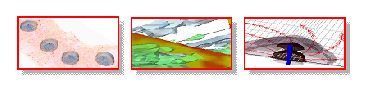
\includegraphics[width=14.0cm]{cg_title_graph_crop}
\end{figure}

\vfill\bigskip
\noindent
% Update instructor list for each course:
Prepared by: \\
Henning Prommer (hp@ekion.com.au) \\
Vincent Post (vincent@edinsi.nl) \\
Douglas B. Kent (dbkent@usgs.gov) \\
Chunmiao Zheng (czheng@ua.edu) \\
James A. Davis (mrwaterx@gmail.com) \\
Olivier Atteia (olivier.atteia@ipb.fr) \\
Bhasker Rathi (bhasker.rathi@gmail.com) \\
Ilka Wallis (ilka.wallis@flinders.edu.au) \\
Janek Greskowiak (janek.greskowiak@uni-oldenburg.de) \\
Pablo Ortega-Tong (portega@intera.com)
%
\tableofcontents%
\mainmatter%
%\selectlanguage{\dutch}%
\pagestyle{fancy} % For nice headers
\fancyfoot{} % Clear current setting
\fancyfoot[LE,RO]{\thepage} % Page number on the left on even pages, to the right on odd pages
\rhead[]{\normalsize\slshape \fancyplain{}{\shorttitle}}    % Right top header
\chapter*{Introduction}

\addcontentsline{toc}{chapter}{Introduction}

\def\shorttitle{Introduction}

Knowledge of the chemistry of groundwater is a requirement for a number of practical purposes. As groundwater is an important source for drinking water, one has to ascertain that its quality is sufficient for consumption. Quality requirements are equally important for other types of utilization such as irrigation or industrial purposes, as well as for the protection of vulnerable ecosystems. More recently, pollution and clean up of aquifers has become a major topic in aqueous geochemistry. Furthermore, understanding of geochemical processes is needed for safety assessment studies, e.g. for the storage of nuclear waste.

Clearly, there are numerous practical applications for aqueous geochemistry. Moreover, geochemistry is an essential tool for understanding the hydrogeological systems that we study. It provides information on the provenance of groundwater, on flow directions and on groundwater ages.

Water quality patterns in aquifers can be complex. The input of different sources of water is the first of factors that adds to this complexity. Sources include precipitation, rivers, lakes (possibly polluted or saline due to strong evaporation), seawater, ascending deep groundwater and anthropogenic sources such as wastewater or irrigation return flow. Geochemical processes add to the complexity since they alter the water's composition as it travels through the subsurface. 
Mineral dissolution and precipitation, 
sorption (transfer of solutes between solution and solids, including ion exchange and surface complexation)
and redox processes (reactions that involve transfer of electrons between chemical species) 
are the 3 main categories of chemical processes 
that determine water quality. Mixing of different water types, which is more a physical than a chemical process, further exerts great influence on the composition of groundwater.

\begin{figure}[tb]
\centering
\includegraphics[width=\textwidth]{custodio}
\caption[Schematic representation of chemical processes that influence the concentration of major ions in coastal areas]{Schematic representation of chemical processes that influence the concentration of major ions in coastal areas \citep{custodio1987}.}
\label{fig:custodio}
\end{figure}

Figure \ref{fig:custodio} illustrates the chemical processes that influence the concentration of the major ions of groundwater as it flows from the recharge area towards the sea. Sulfate (\su) derives from mineral sources such as pyrite and gypsum as well as from seawater and may be lost by conversion to \hs, e.g. by oxidation of organic matter. Bicarbonate (\bi) is formed in the recharge area when \co\ is produced by aerobic respiration and decay of organic matter in the soil zone. Its concentration is further influenced by mineral equilibria (e.g. calcite, dolomite, siderite) and redox reactions that involve sources of organic carbon in the aquifer itself. Sodium (\na) is contained in some silicate minerals that may dissolve but mainly originates from seawater. Cation exchange is the most important chemical process that affects its concentration. Calcite (\cc) is abundant in many geological settings and constitutes the most important source for calcium (\ca) in groundwater. \ca\ also derives from other minerals such as dolomite, gypsum and feldspars and also takes part in cation exchange reactions. Magnesium (\mg) finally, has a high concentration in seawater and is contained in some minerals, the most important being dolomite. Similar to \na\ and \ca\ it can be adsorbed to the exchange complex.

Considering the numerous sources and processes that influence solute concentrations, investigators that try and study the chemistry of aquifers are faced with an overwhelming complexity. Traditional methods that are applied to make sense of the vast pile of numbers that follow from the chemical analyses of water samples involve plotting \citep{fetter2001} and classification of samples into groups \citep[e.g.][]{stuyfzand1993} in order to be able to discern regional trends and to identify chemical processes. No matter how useful these methods are in deriving an idea of the reaction scheme that has given the water sample its composition, they are incapable of determining whether this scheme is feasible from a chemical point of view. In order to check whether a concept obeys basic chemical theory one needs a geochemical model that is based on the firm laws of thermodynamics. Or, as \citet{lichtner96} put it: `Quantitative models force the investigator to validate or invalidate ideas by putting real numbers into an often vague hypothesis and thereby starting the thought process along a path that may result in acceptance, rejection, or modification of the original hypothesis'.

Geochemical models were originally developed in the 1960`s to calculate the speciation dissolved ions. The original models were soon improved and extended to include chemical reactions that alter the water composition such as mineral equilibria and cation exchange \citep{plummer92}. By virtue of the increase in computer computational power it became possible to couple geochemical models with hydrological models to calculate how the water composition changes as it travels through the subsurface \citep{lichtner96}. Today's models have reached a level of sophistication that allows us to simulate real-world processes to understand and explain field observations \citep{lee_windt2001}. 

Elaborate treatment of the basic concepts and applications of aqueous geochemical modeling can be found in for example \citet{bethke1996} and \citet{lichtner96}. This course manual provides a treatment of the basic principles of the models as well as exercises for MT3DMS \citep{zheng99}, PHREEQC \citep{phreeqc2} and PHT3D \citep{prommer_gw}. Extensive use is made of the following packages:

\begin{itemize}

\item PHREEQC for Windows, a graphical user interface for PHREEQC which has the advantage that it's not necessary to switch between programs to create input, perform calculations or view output. The program can be installed on any computer that has Windows95 or higher. It can be obtained for free from:

http://pfw.antipodes.nl/download.html

\item or PHREEQC-3, which can be obtained for free from the USGS website:

http://wwwbrr.cr.usgs.gov/projects/GWC\_coupled/phreeqc/

\item ORTI, an open graphical user interface for reactive transport, including MODFLOW, MT3DMS and PHT3D.

\end{itemize}

\section*{Course outline}
Many students and researchers that are introduced to reactive transport modelling for the first time are overwhelmed by the apparent complexity of it. Mastering the subject requires not only understanding of the underlying theory of groundwater flow, solute transport and hydrochemistry, but also of the many options that the modelling software packages offer. It often takes quite some time before students are confident enough to build and apply their own models. Although reactive transport modelling can indeed be complex, one should not be scared away from it as mastering this subject provides powerful applications. Even the simplest calculations of equilibrium speciation and saturation states already add to the knowledge of and insight in the chemical system that is being studied. Each student in hydrochemistry should therefore have at least basic knowledge of aqueous geochemical models.

This course guide is a step by step introduction of the topic of reactive transport modelling. It is assumed that the reader has some knowledge of hydrochemistry, which is indispensible for successful application of the models. The first chapter introduces the basic theory of geochemical models and familiarizes the reader with PHREEQC by using simple example exercises. Each successive chapter discusses additional theory and the exercises increase in complexity. After having worked through the entire course guide, the student has enough theoretical background and practical experience to build his or her own models and apply these to real-world problems.


\lhead[\normalsize\slshape\fancyplain{}{Chapter \thechapter}]{} % Left top header
\thispagestyle{empty} % Suppress page number on separator page

%\include{physical/single_spec_2D_orti}
\include{physical/single_spec_2D_ipht3d}
\include{equilibrium/text_kigam2019}
%\chapter{Physical processes affecting water chemistry: Mixing and evaporation}
\def\shorttitle{Mixing and evaporation} % Abbreviated chapter title for right top header

\section{Evaporation}

\subsection{Exercise: evaporation of acid rain}
When rain falls its concentration is increased by interception and evapotranspiration before it recharges groundwater. Evaporation is easily modelled in PHREEQC by simply removing \wa. In this exercise, evapotranspiration increases concentrations by a factor of 1.5 and the sample is brought in equilibrium with gibbsite and atmospheric oxygen. This increases the concentrations of \al\ and oxidises all \nh\ to \no.

The input file for this exercise is `klosterhede.phrq'. The composition of solution 1 represent throughfall at Klosterhede, Denmark (Hansen and Postma, 1995).

\begin{quote}
\# Acidification, ... throughfall concentrated 1.5 times \\
\# \\
SOLUTION 1	\# Throughfall at Klosterhede \\
	temp	10 \\
	pH	 4.33	charge \# Measured pH =4.33, lowered by NH4+ to NO3- \\
	pe	10.0	O2(g)	-0.66 \\
	units	umol/kgw \\
	Na	986. \\
	K	100. \\
	Mg	127. \\
	Ca	 54. \\
 \\
	Cl	1080. \\
	N(5)	 221.	\# sum of NH4+ and NO3- \\
	S(6)	 154. \\
REACTION 1 \\
	H2O	-1.0 \\
	18.503		\# Concentrate 1.5*, remove 1/3 of H2O \\
SAVE solution 2 \\
END \\
MIX \\
	2	1.5	\# Make volume up to 1 kg water \\
EQUILIBRIUM\_PHASES 2 \\
	Gibbsite   0.29 \\
	O2(g)	  -0.66 \\
SELECTED\_OUTPUT \\
    -file klost\_dk.prn \\
    -reset false \\
    -sim true \\
    -pH true \\
    -pe true \\
    -mol O2 \\
USER\_PUNCH \\
    -heading m\_NO3 mg\_Al/l \\
    -start \\
    10 PUNCH MOL("NO3-") \\
    20 PUNCH  \\
    -end \\
END
\end{quote}

By default, a solution in PHREEQC has a mass of 1 kg. Concentrating the solutes by a factor of 1.5 corresponds to removing 1/3 of the \wa. One kilogram of water contains 55.5 moles of \wa\, so $1/3 \cdot 55.5 = 18.52$ moles have to be removed. To restore the total amount of solution to 1 kg again, the keyword \textbf{MIX} is used. Following the MIX keyword is a list of solution numbers (number 2 in this case) and their fraction in the mixture. A fraction of 1.5 corresponds to a mulitplication of all the concentrations of the solution (also that of \wa) by 1.5.

The keywords \textbf{SELECTED\_OUTPUT} and \textbf{USER\_PUNCH} control the output that is written to the file `klost\_dk.prn'. The standard PHREEQC output file can become quite large and is not easily read in a spreadsheet. The \textbf{SELECTED\_OUTPUT} keyword can be used to create output files in a spreadsheet format. The \textbf{-reset} identifier is set to false, which means that the default output options are turned of. The identifiers on the next lines specify that only the simulation number, pH, pe and the concentration of \ox\ are written to the file.

The \textbf{USER\_PUNCH} keyword is slightly more complicated. It uses BASIC statements to control the output. The identifier \textbf{-headings} is used to specify the column headings that will appear above the numbers in the file. The identifiers \textbf{-start} and \textbf{-end} surround the block of BASIC statements. The lines with the BASIC statements have to be numbered in ascending order. A special PHREEQC BASIC statement PUNCH writes a number to the output file. An other special PHREEQC statement is MOL, which is used to get the molar concentration of a species, \no\ in this example. Try to see if you can complete the BASIC statements to write the total Al concentration in mg/l to the output file. Hints: the total concentration is obtained with the TOT("") BASIC statement. You can directly recalculate the concentration using formulas and the gram formula weight of Al can be found in the database.

The pH after concentrating is \ldots\ldots. Now impose equilibrium with gibbsite so that pH changes to \ldots\ldots (field data indicate the porewater to be in equilibrium with slightly more soluble \gi, therefore SI is set to 0.29). The pH increase is due to the reaction:

 \ldots\ldots

The \al\ concentration is:  \ldots\ldots mg/l.

Repeat the same calculation for a `dry' year. In a dry year the solutes are concentrated 4 times. Thus, \ldots\ldots moles of \wa\ is removed from 1 kg of solution. The pH now becomes \ldots\ldots. With MIX the concentrated solution is brought to 1 kgw. Equilibrium with gibbsite gives a pH = \ldots\ldots and \al\ = \ldots\ldots mg/l. How does this compare to the maximum allowable concentration of Al in drinking water, which is 0.2 mg/l?

%\chapter[Reactive transport with PHT3D]{Reactive transport with PHT3D}
\def\shorttitle{Reactive transport with PHT3D} % Abbreviated chapter title for right top header

In this chapter we introduce coupled modelling of mass transport and geochemical reactions.
While different modelling approaches for the simulation of such reactive transport 
problems exist, we will focus our discussion on the PHT3D model, which
combines the two existing models MT3DMS and PHREEQC-2 through 
a split-operator technique \citep[]{herzer89,phdzysset}.
This technique has more or less become the standard method for solving such combined
physico-biogeochemical problems. The technique involves separating
the processes (e.g., flow, transport of individual chemical
components/species, chemical reactions, microbial activity) within
the numerical model and solving each sub-model independently. The
technique enables use of available, well tested, transport, flow
and reaction packages, as well as associated GUIs for setting up
problems. Within the PHT3D simulator MT3DMS and PHREEQC-2 solve two 
different sets of equations: one for hydrological solute transport and 
one for the chemical reactions. MT3DMS is used to solve the solute 
transport part and PHREEQC-2 computes the concentration changes
that are caused by geocchemical reactions. 

\section{Solute transport}

The reactive transport equation (solved by MT3DMS) for the
$i^{th}$ (mobile) aqueous component is (in indical notation):
\begin{equation}
{\frac{\partial C_i} {\partial t} = \frac{\partial} {\partial
x_{\alpha}}
 (D_{\alpha\beta} \frac{\partial C_i} {\partial x_{\beta}}) -
 \frac{\partial} {\partial x_{\alpha}} (v_{\alpha} C_i) + \frac{q_s C^s_i}{\theta} + r_{reac,i}}
\label{eq:ad_reac_mobile}
\end{equation}
and for immobile entities, e.g., minerals:
\begin{equation}
{\frac{\partial C_i} {\partial t} = r_{reac,i}}
\label{eq:ad_reac_immobile}
\end{equation}

where $v_{\alpha}$ is the pore-water velocity in direction
$x_{\alpha}$, $D_{\alpha\beta}$ is the hydrodynamic dispersion
coefficient tensor, $q_s$ is a volumetric flow rate per unit
volume of aquifer representing fluid sources (positive) and sinks
(negative), $\theta$ is the porosity of the subsurface medium,
$C^s_i$ is the concentration of the source or sink flux,
$r_{reac,i}$ is a source/sink rate due to chemical reaction and
$C_i$ is the total aqueous component concentration of the $i^{th}$
component \cite[]{yehtri89,enges92}. There $C_i$ is defined as:
\begin{equation}s
{C_i = c_i + \sum_{j=1,n_s} \ Y_{j}^s s_j}  
\label{eq:cj}
\end{equation}
where $c_i$ is the molar concentration of the (uncomplexed)
$i^{th}$ aqueous component, $n_s$ is the number of species in
dissolved form that have complexed with the aqueous component,
$Y_j^s$  is the stoichiometric coefficient of the aqueous
component in the $j^{th}$ complexed species and $s_j$ is the molar
concentration of the $j^{th}$ complexed species.

In the current PHT3D version the (local) redox-state, $p$e, is
modeled by transporting chemicals/components in different redox
states separately, while the $p$H is modeled from the (local)
charge balance. Using a sequential operator-splitting technique
\cite[]{herzer89,val92,miller93,phdzysset,zysset94_2,morka95_1,morka95_2,
barry96,barry97,steefel96} the advection and dispersion terms
within (\ref{eq:ad_reac_mobile}) are solved by the transport
module MT3DMS for $n_{tot}$ components and for each time step of a
temporally discretised problem, with
\begin{equation}
n_{tot} = n_{e,nre} + \sum_{l = 1,n_{e,re}}{n_{rs,l}}  \
\label{eq:ntot_manual}
\end{equation}
where $n_{e,nre}$ is the number of (mobile) chemical elements
occurring in only one redox state, $n_{e,re}$ is the number of
elements occurring in multiple redox states and $n_{rs,l}$ is the
appropriate number of different possible redox states of the
$i^{th}$ element. In other words, if chemical elements occur in
multiple, i.e., $n_{rs,l}$ different redox states within a
simulation problem, an appropriate, higher number of separate
transport equations needs to be solved in order to accurately
predict the redox state ($p$e). For example, hydrological
transport of iron-complexes would typically require modelling the
total aqueous component concentrations of $Fe(II)$ and $Fe(III)$
complexes separately.

\section{Geochemical Reactions}

In PHT3D all concentration changes of aqueous components and
immobile entities that result from reactive processes are computed
by PHREEQC-2. It is, in contrast to its precursor models PHREEQE
\cite[]{parkhurst80} and PHREEQC \cite[]{parkhurst95}, capable of
simultaneously solving arbitrary, kinetically controlled reactions
in addition to geochemical equilibrium problems. From the full set
of geochemical reactions that can be handled by PHREEQC-2, a
subset, including aqueous complexation, mineral
precipitation/dissolution, and ion exchange has been implemented
into the present version of PHT3D. This subset will be sufficient
for most subsurface reaction/transport simulation problems.
However, some limitations remain, as will be discussed in
\ref{limit}.

\section{Coupling Procedure}
\label{sec:coupling} Several options to couple transport and
reactive processes through split-ope\-ra\-tor methods exist, e.g.,
sequential, alternating and iterative split-operator methods.
Details of the different techniques have been discussed, e.g., by
\cite{herzer89}, \cite{val92}, \cite{miller93}, \cite{phdzysset},
\cite{zysset94_2}, \cite{morka95_1,morka95_2}, \cite{steefel96}
and \cite{barry96,barry97,barry2002}. In PHT3D a slightly modified
version of the 'standard' sequential split-operator method
described by \cite{walt94a} has been implemented. A
time-discretised form of (\ref{eq:ad_reac_mobile}) for reactive
transport of a component, as defined by (\ref{eq:cj}) is:
\begin{equation}
C_i^{k+1} - C_i^k = L(C_i)^{k+1/2} \ \Delta t + R_{reac,i}\
\label{eq:ss_discretinorg}
\end{equation}
where $L(C_i)^{k+1/2}$ ($ML^{-3}$) is the spatial differential
operator (central in time, i.e., time level $k+1/2$) and $C_i^k$
and $C_i^{k+1}$ ($ML^{-3}$) are the total aqueous component
concentrations of the $i^{th}$ component at the old time level $k$
and the new time level $k+1$, respectively, $\Delta t$ is the time
step length, and $R_{reac,i}$ ($ML^{-3}$) is the difference in
concentrations from before and after a reaction step. In the model
presented by \cite{walt94a}, $R_{reac,i}$ represents the relative
mass of a component generated or consumed instantaneously by an
equilibration of the aqueous solution with a mineral assemblage at
the time $t^{equil}$ ($t^k \le t^{equil} \le t^{k+1}$),
compensating for the chemical pertubation arising from advective
and dispersive transport during $\Delta t$. However, in PHT3D
$R_{reac,i}$ does not only represent concentration changes of
aqueous components due to (equilibrium) precipitation/dissolution
reactions, but also due to any other reactive process handled by
PHREEQC-2, such as ion exchange, biodegradation, etc., depending
on which reactions the $i^{th}$ component participates in. The
concentration change $R_{reac,i}$ might occur as a result of
equilibrium, kinetic or mixed equilibrium/kinetic reactions. In
PHT3D, the (MT3DMS) advection and dispersion modules solve the
concentrations $C_i^{trans}$, i.e., the concentrations at the new
time level $k+1$ that result from physical transport only:
\begin{equation}
C_i^{trans} = L(C_i)^{k+1/2} \ \Delta t + C_i^k\ \label{eq:seq_1}
\end{equation}
for the $n_{tot}$ compounds/components. In contrast to
\cite[]{walt94a} and depending on the actual advection scheme
selected for a simulation (FD, TVD, MOC, MMOC or HMOC), the
transport simulator MT3DMS may further sub-divide the user-defined
time step length $\Delta t$ into several transport steps that
fulfil the relevant stability and/or accuracy criteria for
physical transport (Courant number). Thus, sometimes several
subsequent transport steps (without reactions) might be carried
out by MT3DMS to compute $C_i^{trans}$. Once $C_i^{trans}$ is
computed, the second step, which models the reaction(s), will be
carried out in a sequential manner for each grid cell
individually. The computation of the reaction step within a grid
cell is independent from concentrations at neighboring cells. This
then leads to the concentrations $C_i^{k+1}$ at the new time level
$k+1$, i.e.,
\begin{equation}
C_i^{k+1} = C_i^{trans} + R_{reac,i}\ \label{eq:seq_2}
\end{equation}
For the computation of the source/sink term $R_{reac,i}$, the
concentrations $C_i^{trans}$ from after the transport step(s) are
used as initial concentrations for the chemistry calculation step.
The time step length for the reaction simulation will correspond
to the user-defined time step length $\Delta t$ and not to the
automatically selected transport step size, which depends on the
actual advection scheme used for a simulation. For the computation
of kinetic reactions PHREEQC-2 uses a $5^{th}$ order integration
scheme \cite[]{fehlberg69} which, if a specified tolerance is not
met for the error estimate of the integration, will automatically
subdivide the user-defined time step length $\Delta t$. In that
case, the user-defined time step will be numerically integrated
over two or more subintervals, each of which is integrated with
the $5^{th}$ order integration scheme. Through this procedure the
kinetic reactions are assured to be integrated accurately over the
user-defined time interval. Of course, an increased temporal
splitting error will occur compared to a scheme where transport
and reactions steps alternate more often, e.g., at the frequency
dictated by the transport step size.

However, the model execution times, i.e., CPU-times of the present
scheme can be significantly lower, which often is helpful,
particularly in the early, more conceptual stages of a modelling
project, i.e., where (very high) solution accuracy is not a
primary concern. Accuracy can be improved by reducing the size of
$\Delta t$. For a small enough step size the numerical solution
will become independent of $\Delta t$ as a result of a negligible
splitting error.

In order to reduce computational load, a further optional
modification of the 'standard' sequential split-ope\-ra\-tor
tech\-nique was implemented in PHT3D. The modification allows the
reaction step to be temporally omitted in cells where no reactive
changes are expected. This modification exploits the fact that in
many model applications there may exist zones, sometimes large,
within the model domain where chemical gradients are negligible
between neighbouring grid-cells and where the aqueous solution is
in equilibrium with the mineral assemblage and the cation-exchange
sites. In these zones the reaction term $r_{reac}$ computed by
PHREEQC-2 might be zero for significant portions of the total
simulation time and thus the reaction step, in principle, can be
omitted during these periods. A typical case where this applies is
a steadily spreading point source contamination within an
initially, chemically homogeneous, equilibrated multi-dimensional
model domain, where in the early stages of the simulation
geochemical changes occur in a very small portion of the aquifer.
This concerns in particular cases where advection is the dominant
transport mechanism. To decide whether the reaction step in a
particular grid-cell can be omitted, the joint fulfilment of the
two criteria (three-dimensional case):
\begin{equation}
  {\sum_{k = lay-2}^{lay+2}\sum_{l=col-2}^{col+2}\sum_{m=row-2}^{row+2}\sum_{i=1}^{n_{tot}}
\ \ \mid r_{reac_{k,l,m,i}} \mid \ \ < \ \epsilon_{aqu}
\ \ \ \ \ \ \ \ \ \ \ \ \ \ \ \ \ \ \ \ }
\label{eq:phcact_dis}
\end{equation}
and
\begin{equation}
  {{\sum_{k = lay-2}^{lay+2}\sum_{l=col-2}^{col+2}\sum_{m=row-2}^{row+2}
r_{reac_{k,l,m,pH}}} \ < \ \epsilon_{pH} \ \ \ \ \ \ \ \ \ \ \ \ \
\ \ \ \ \ \ \ }
\label{eq:phcact_ph}
\end{equation}
with
\begin{equation*}
  { 3 \leq k \leq lay_{max}-2, \\
    3 \leq l \leq col_{max}-2, \\
    3 \leq m \leq row_{max}-2   }
\end{equation*}
has been found to be an efficient test, where $r_{reac_{k,l,m,i}}$
is the computed reaction term for the $i^{th}$ component in layer
$k$, column $l$ and row $m$, both $\epsilon_{aqu}$ and
$\epsilon_{pH}$ are user-defined accuracy criteria, $lay$, $col$,
and $row$ are the indices of the layer, column and row of the
(tested) grid-cell, respectively, and $lay_{max}$, $col_{max}$ and
$row_{max}$ are the total numbers of layers, columns and rows,
respectively in the model. The criteria (\ref{eq:phcact_dis}) and
(\ref{eq:phcact_ph}) are tested for each grid-cell after a
PHREEQC-2 reaction step. If both are fulfilled for a grid-cell,
the execution of PHREEQC-2 (but not physical transport) is
deactivated in this cell until it is reactivated.

Reactivation occurs automatically when either criterion
(\ref{eq:phcact_dis}) or (\ref{eq:phcact_ph}) is not fulfilled,
i.e., if reactive changes occur in neighbouring grid cells. Note,
that (\ref{eq:phcact_dis}) does not only include the directly
adjacent cells but also cells that are two layers, two columns or
two rows away. Grid-cells that receive external fluxes (e.g.,
through wells, rivers, recharge, \ldots{}) can not be deactivated and,
furthermore, reaction simulations are always carried out for all
grid-cells at the beginning of each new stress period, including
the very first time step of the first stress period. For certain
simulation problems, such as those where the initial aqueous
solution and/or the inflow solution across model boundaries are
not in equilibrium with the mineral assemblage and mineral
reactions are kinetically controlled, $r_{reac}$ might always be
non-zero in most or all grid-cells.

\section{Program design}
The coupling between MT3DMS and PHREEQC-2 was achieved by several
new subroutines that enable the communication between the two
programs. The MT3DMS code, written in Fortran 90, was used as the
driver program, i.e., the main program, whereas the original
PHREEQC-2 main program, written in the C programming language, has
become a subroutine of MT3DMS. The new additional subroutines,
called by MT3DMS, were also written in the C programming language.
Despite the addition of those new subroutines, the original main
model structures of both models, MT3DMS and PHREEQC-2 was largely
maintained. This bears the notable advantage that future, modified
and improved versions of the two underlying models can be quickly
implemented with a modest effort. The disadvantage of this 'loose'
coupling strategy is the loss of some computational efficiency as
a result of occasional increased overhead, e.g., through the
repeated reading and interpretation of the same database file and
through partial data-communication via ASCII-files. Figure
\ref{fig_pht3d_flowchart_a} shows a flowchart of the PHT3D main
program that indicates the main modifications that were made
compared to the original MT3DMS code. As can be seen in the chart,
the PHT3D-specific modifications concern the
\begin{itemize}
\item data preparation where the new subroutine \textbf{MCRP} is called.
\item newly added subroutines \textbf{PREPH}, \textbf{PHMAIN} and \textbf{POSTPH2}, which
preprocess, execute and postprocess, respectively, the PHREEQC-2 reaction step
\item the newly added subroutine \textbf{PHCACT} which decides after each reaction step
for which grid-cells a reaction simulation will be necessary during the next reaction step.
\end{itemize}

\begin{figure}
\begin{center}
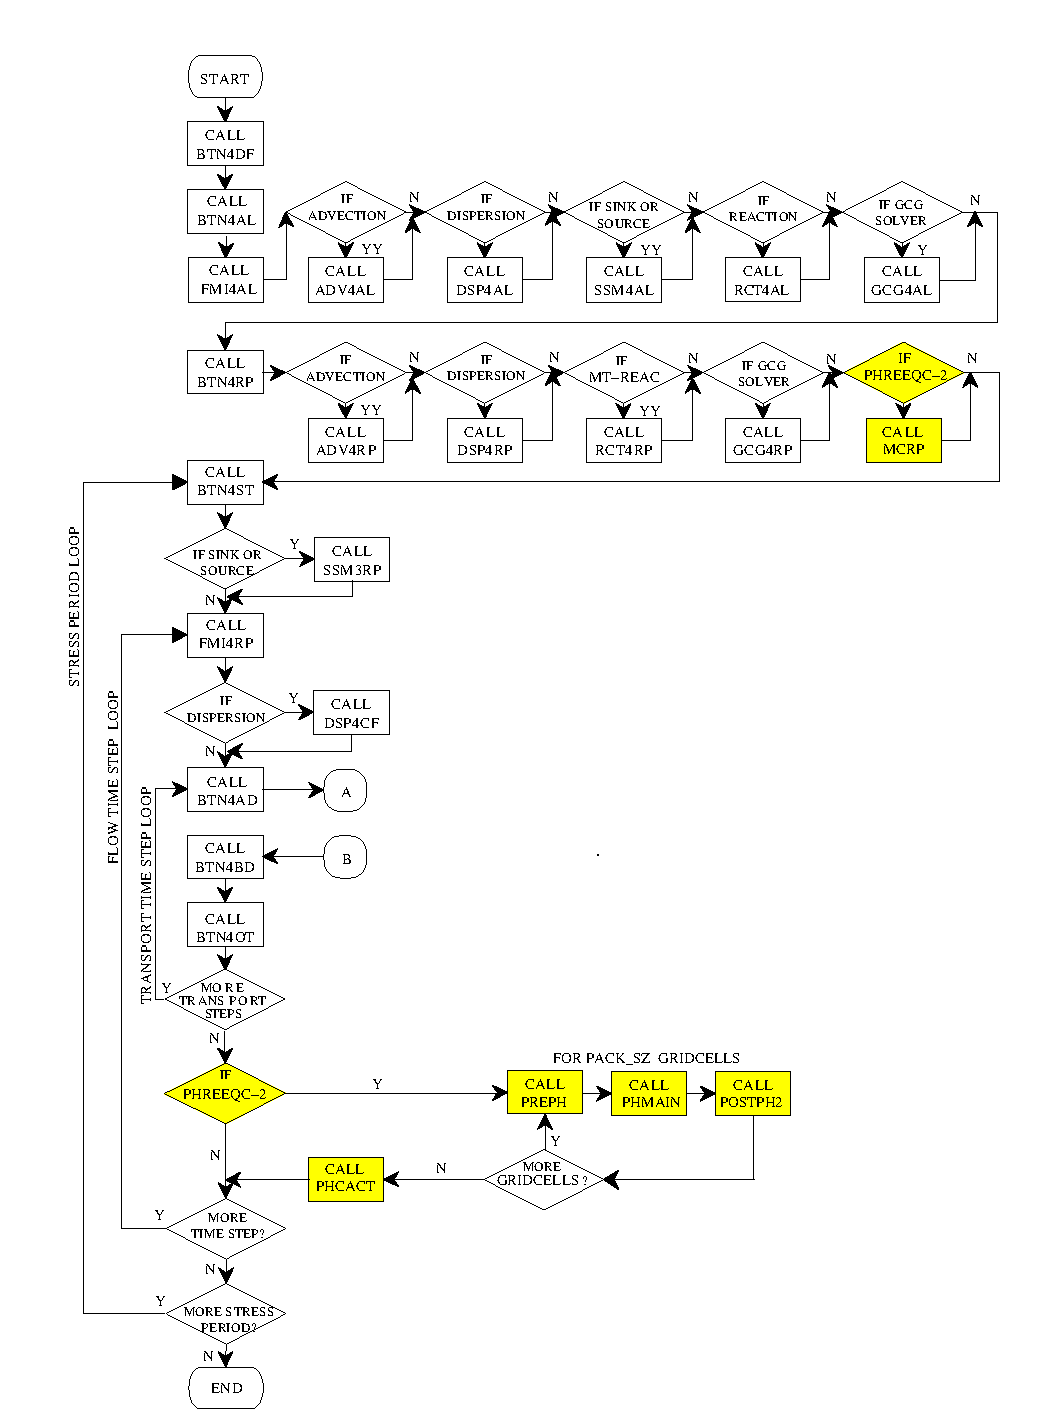
\epsfig{file=pht3d_flowchart_d.eps,width =10.cm ,angle=0,clip=}
\end{center}
\caption[Flowchart of the main program of PHT3D]{Flowchart of the main
program of PHT3D, modified from \citep[]{zheng99}.
The PHT3D-specific changes of the original MT3DMS code are marked in yellow.}
\label{fig_pht3d_flowchart_a}
\end{figure}

As part of the initial data preparation procedure, the MT3DMS main
program calls the newly added \textbf{MCRP} subroutine in PHT3D.
During the execution of this subroutine the PHREEQC-2 interface
package file {\color{red} \textbf{pht3d\_ph.dat}} is read and the
input data are prepared for their use in other PHT3D-specific
subroutines. For example, the subroutine reads, sorts and stores
the number and names of entities included in a simulation and
allocates a unique species number to each of those entities. Given
by the structure of MT3DMS, mobile entities will form the first
'block' of species, followed by immobile entities such as
minerals, immobile bacteria or (immobile) NAPL compounds which
form the second 'block'.

In the course of a model simulation, i.e., during each reaction
step, the three subroutines \textbf{PREPH}, \textbf{PHMAIN} and
\textbf{POSTPH2} preprocess, execute and postprocess the PHREEQC-2
simulations that compute the reaction terms. In detail, the
subroutine \textbf{PREPH}
\begin{itemize}
\item reads the concentrations of all entities from the
appropriate MT3DMS arrays and \item generates an ASCII file
{\color{red} \textbf{phinp.dat}} that will subsequently serve as
input file for PHREEQC-2.
\end{itemize}
Following the creation of {\color{red} \textbf{phinp.dat}}, the
execution of the \textbf{PHMAIN} subroutine (a modified version of
the original PHREEQC-2 \textbf{MAIN} program)
\begin{itemize}
\item performs the computation of the reaction step using
{\color{red} \textbf{phinp.dat}} and the database file
{\color{red} \textbf{pht3d\_datab.dat}} as input files and \item
writes the newly computed concentrations to the file
{\color{red} \textbf{phout\_sel.dat}}, an ASCII file produced by
and during the execution of PHREEQC-2. It contains all relevant
simulation results, i.e., the newly computed concentrations of
mobile and immobile chemicals from after the reaction calculation.
\end{itemize}
Subsequently, the subroutine \textbf{POSTPH2} will
\begin{itemize}
\item read the output file {\color{red} \textbf{phout\_sel.dat}}
that contains those newly computed concentrations \item compute
the concentration changes from before and after the reaction
simulation, i.e., the reaction term $r_{reac}$ \item save the
newly computed concentrations in the appropriate MT3DMS data
arrays.
\end{itemize}
The three above steps/subroutines might be carried out only once
for all $n_{grid,max}$ (= $lay_{max} \times col_{max} \times
row_{max}$) grid-cells of the model domain or, alternatively,
repeatedly for several packets of a user-defined maximum number of
grid-cells.

At the end of each reaction step, i.e., once the reaction terms
$r_{reac}$ are known for all $n_{grid,max}$ grid-cells, the
subroutine \textbf{PHCACT} is invoked to check whether the
criteria defined by equations (\ref{eq:phcact_dis}) and
(\ref{eq:phcact_ph}) are fulfilled and appropriate internal flags
are set for each grid-cell. The settings will be used during the
reaction simulation of the next time step.

\section{Model Structure} 
For the development of PHT3D, the original MT3DMS model has been 
used as a basis to incorporate an interface that prepares and executes 
the PHREEQC-2 reaction step. This model interface was kept relatively 
simple which has the notable advantage that future, modified and 
improved versions of not only the transport model, but also 
the geochemical model, can be quickly implemented with a modest effort. 
The model input/output for the existing MT3DMS features has not been changed. 
Compared to a standard MT3DMS simulation, only two additional input files 
are needed, one which contains information such as the names and types 
of chemicals, parameter values, and the stoichiometry of 
kinetic reactions and a second file that contains the definition 
of both equilibrium and kinetic reactions. The syntax of the 
latter file is analogous to that one used by the 
original PHREEQC-2 database file. Figure \ref{fig:data_flow} shows the data flow within a typical PHT3D application.


\begin{figure}[ht]
\centering
%\includegraphics[width=10cm,bb=42 0 450 250]{pht3d_data_flow.png}
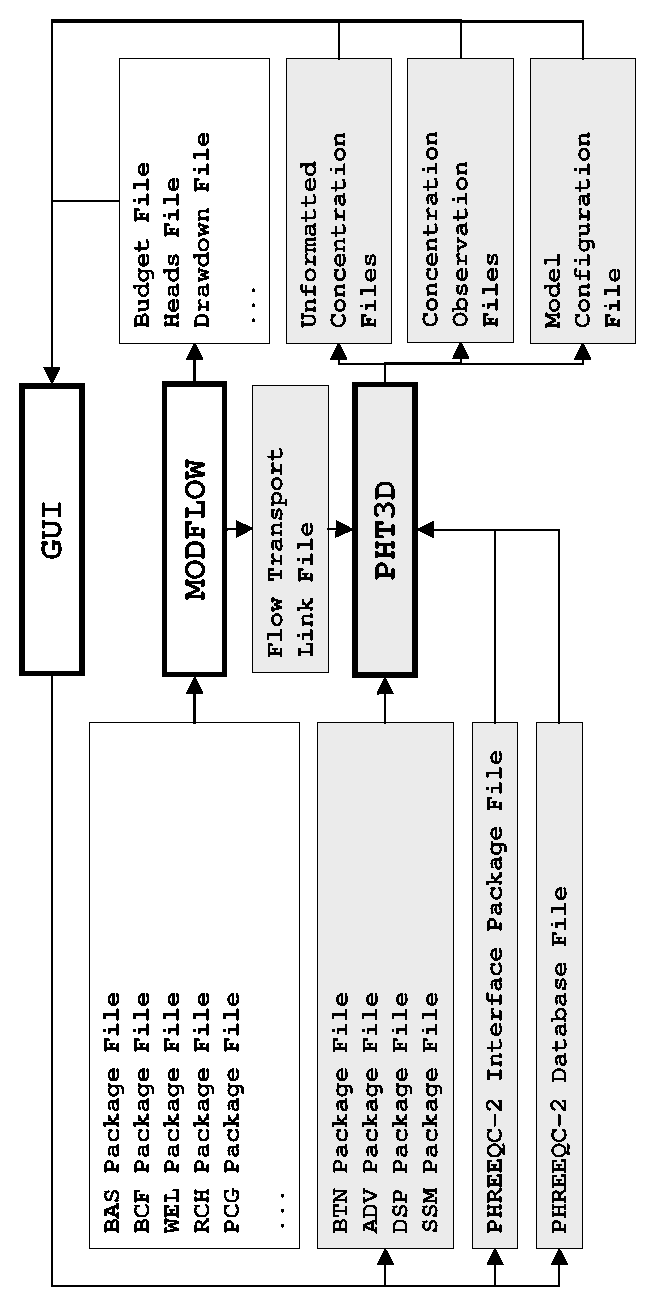
\includegraphics[height=10.5cm, angle=270]{data_flow.eps}
\caption[Data flow in a MODFLOW-based PHT3D simulation.]{Data flow in a MODFLOW-based PHT3D simulation.}
\label{fig:data_flow}
\end{figure}


\section{Limitations} \label{limit}

Only a subset, but not all of the geochemical reactions that can
be computed with the original PHREEQC-2 model is currently
supported by PHT3D. Among those unsupported reactive processes is
the surface complexation model (SCM) which, in some cases, might
be essential to simulate the mobility of ions, e.g., of trace
metals, accurately. While the SCM is not included in the present
version, it is planned to be incorporated into future
versions of PHT3D.

As in the original MT3DMS model and other MT3DMS-based package,
PHT3D simulations are carried out on the base of a flow-field
computed beforehand by a separate flow simulator, typically
MODFLOW. Thus, it can't reproduce the potential impact of reactive
processes on the groundwater flow field and the model is not
suitable to predict, for example, the impact of bioclogging or
mineral precipitation on the hydraulic properties of an aquifer.

Note also that the use of the implicit GCG solver is currently not supported.
Furthermore, the simultaneous use of the MT3DMS chemical reaction
package and PHREEQC-2 as reaction simulator was not tested.

\section{Additional literature}

More detailed information about the PHT3D model and several application 
examples can be found in \cite{pht3d} and in \cite{prommer_gw}. Excellent introductions
into the general area of reactive transport are provided by \cite{steefel96} and by \cite{ap2005}. 


\chapter[Mineral dissolution and precipitation]{Mineral dissolution and precipitation}
\def\shorttitle{Mineral dissolution and precipitation} 

\section[Simulating mineral- and gas-phase equilibria in PHREEQC]{Simulating mineral- and gas-phase equilibria in PHREEQC}

In aqueous speciation simulations in PHREEQC using, e.g., the {\color{red} \textbf{SOLUTION}} 
keyword, mineral saturation indices and gas-phase 
saturation indices (the log of the partial pressure of the gas phase) 
are reported to the output file.  
Now we will allow mass transfer of solutes from or to the aqueous phase to or from solid phases 
if their formation or dissolution is thermodynamically favorable. 
Also, mass transfer of solutes from/to solution to/from the gas phase 
will be allowed if thermodynamically favorable.

Thermodynamic data for phases are entered using the keyword {\color{red} \textbf{PHASES}}.  
The minimum information provided under the {\color{red} \textbf{PHASES}} keyword is:

\begin{quote}
{\color{red}PHASES \\
Phase-name \\
Reaction formula \\
logK (25 $^\circ$C) }\\
\end{quote} 

The phase-name is, of course, the name of the phase. Important examples for often used phases include: \\
$Goethite$, $Fe(OH)3(a)$, and $O2(g)$, corresponding to $\alpha$-FeOOH, amorphous hydrous ferric oxide, 
and oxygen in the gas phase, respectively.  
The reaction formula must be written with the phase on the left-hand side of the equation 
and the aqueous species on the right-hand side of the equation.  
The equilibrium constant at 25 $^\circ$C must also be provided.  
Additional data can be provided, such as the effect of temperature on the 
equilibrium constant and the molar volume (in PHREEQC version 3.x) 
as a function of temperature. For a complete description, 
consult the PHREEQC manual (or on-line users guide) under 
'Description of Input for the PHASES keyword'.  
For the three examples above, entries might look like:


\begin{quote}
{\color{red}PHASES \\
Goethite \\
FeOOH  +  3H+  =  Fe+3  +  2H2O \\
-log\_k	-1.0 \\
\\
Fe(OH)3(am) \\
Fe(OH)3  +  3H+  =  Fe+3  +  3H2O \\
-log\_k	4.891 \\
\\
O2(g) \\
O2  =  O2 \\
-log\_k	-2.8983 }\\
\end{quote} 

Note that in the reaction for $O2(g)$, the O2 on the left-hand side of the reaction 
refers to O2 in the gas phase and the O2 on the right-hand side of 
the reaction refers to O2 in the aqueous phase.

The keyword that allows mass transfer into or out of the aqueous phase into gas 
and solid phases is {\color{red} \textbf{EQUILIBRIUM\_PHASES n}}. 
Like with the {\color{red} \textbf{SOLUTION}} keyword we can define multiple 
{\color{red} \textbf{EQUILIBRIUM\_PHASE}} assemblages using an index, represented by n.  
Following the description in the PHREEQC manual, the syntax is:

\begin{quote}
{\color{red}EQUILIBRIUM\_PHASES n \\
Phase-name	SI	Chemical-formula	Initial-mass} \\
\end{quote}

The {\color{red} \textbf{Phase-name}} is the name of the phase, exactly as it appears under the 
{\color{red} \textbf{PHASES}} keyword in the database or input file.  
The {\color{red} \textbf{SI}} is the saturation index at which PHREEQC will cause mass transfer to occur.  
For solid phases we typically use 0, allowing mass transfer 
to occur until complete equilibrium with respect to that mineral is achieved, i.e., SI = 0.  

\par For gas-phase constituents, using the log of the partial pressure of the constituent 
in the atmosphere will allow mass transfer to occur once the aqueous-phase composition 
is in equilibrium with the atmosphere. 
The {\color{red} \textbf{chemical-formula}} provides the chemical formula used to effect mass transfer.  
Typically we use the chemical formula of the mineral or the gas-phase constituent, 
in which case no entry is required since that is the default.  
However, we might need to use a different formula.  
For example, if there is carbonate in the aqueous solution we might want Ca for calcite formation 
to come from dissolution of plagioclase feldspar or gypsum.  
The {\color{red} \textbf{initial-mass}} is the initial mass of the phase in the system.  
The initial mass must be in moles, i.e., {\color{red} \textbf{it is not given as mass per volume of water !}}.  
If the phase is not present initially but we want it to form 
if it becomes supersaturated, we would enter 0 for the initial mass.


\begin{table}[h]
\topcaption{PHREEQC keywords used for allowing mass transfer of solutes to/from the aqueous phase.}
\centering
\footnotesize
\begin{tabular}{llll}
\toprule
Constituents	& Database	                & Input	     & Selected\_Output   \\ \hline
Aqueous       &	SOLUTION\_MASTER\_SPECIES & SOLUTION n & Totals (e.g., Ca)   \\
              & SOLUTION\_SPECIES	        & MIX n      & Molalities (e.g., $Ca^{+2}$) \\
              &                           &            & Activities (e.g., $Ca^{+2}$) \\
              &                           &            & Saturation\_index  \\
              &                           &            & USER\_PUNCH       \\
              &                           &            &        SC         \\
              &                           &            &     Rho           \\
              &                           &            &   Soln\_Vol        \\ \hline
Gas phase	    & Phases	   & EQUILIBRIUM\_PHASES n   & EQUILIBRIUM\_PHASES \\
              &            &                         & USER\_PUNCH   \\
              &            &                         & EQUI(...)     \\ \hline
Solid phase	  & Phases     & EQUILIBRIUM\_PHASES n   & See Gas Phase \\ \hline
Surface       & SURFACE\_MASTER\_SPECIES & SURFACE n & See aqueous   \\
complexation  & SURFACE\_SPECIES         &           &       \\ \hline
Other         &                          &           &       \\ \hline
SAVE, USE	    & Solution n,              &           &       \\
              & EQUILIBRIUM\_PHASES n    &           &       \\ 
							& SURFACE n                &           &       \\ 
\bottomrule
\label{tab:keywords_mass_transfer}
\end{tabular}
\end{table}	


\section[PHREEQC Exercise 3: Phase Equilibria]{PHREEQC Exercise 3: Phase Equilibria}
\subsection[Simulating mineral equilibria]{Simulating mineral equilibria}

Here are a few very simple examples that illustrate how we can use the 
{\color{red} \textbf{EQUILIBRIUM\_PHASES}} n keyword.

\begin{itemize}
\item Dissolve 0.001 moles of calcite in 1 liter of 0.01 mol/L NaCl.

\item Using the {\color{red} \textbf{SOLUTION}} n keyword, make a solution of 0.01 mol/L NaCl at 21 $^\circ$C. Using the {\color{red} \textbf{EQUILIBRIUM\_PHASES n}} keyword, equilibrate that solution with 0.0001 moles (10 mg) of calcite. What happens?

\end{itemize}

\begin{quote}
{\color{red}SOLUTION 1 \\ 
Temp	21 \\
pH	7 charge \\
units  mol/L \\
Na  0.01 \\
Cl  0.01 \\
\# \\
EQUILIBRIUM\_PHASES 1 \
Calcite  0.  0.0001 \\
\# Phase-name.  Must agree with the name in the database \\
\# Saturation index \\
\# moles of calcite initially present. \\
END }\\
\end{quote}

\begin{itemize}
\item Does all the calcite dissolve? 
\item Increase the amount of calcite until there is enough to saturate the solution. How much calcite does it take to saturate a solution with 0.01 M NaCl ?

\item Now add 0.0001 moles of calcite and 0.01 moles of gypsum to a 0.01 M NaCl solution 
using the {\color{red} \textbf{EQUILIBRIUM\_PHASES}} keyword. Now how much calcite dissolves ?

\item Equilibrate 0.01 M NaCl at 21 C with 0.01 moles of aragonite then allow calcite to precipitate until equilibrium is achieved.
There are two approaches. First, set up the simulation with a single {\color{red} \textbf{EQUILIBRIUM\_PHASES n}} data block that has an excess of aragonite and initially no calcite.

\end{itemize}

\begin{quote}
{\color{red}SOLUTION 1 \\
... \\
EQUILIBRIUM\_PHASES 1 \\
Aragonite  0 0.01 \\
Calcite  0  0 \\
\# Note that the phase names need to match those in the database. \\
\# Initially 0.01 moles of aragonite is present. \\
\# No calcite is present initially. \\
END}
\end{quote}

\begin{itemize}
\item Second, run the simulation in two steps. In the first step, 0.01 M NaCl is equilibrated with 0.01 moles of aragonite. The resulting solution composition is saved using the {\color{red} \textbf{SAVE}} keyword.  After the end of the first simulation (marked by {\color{red} \textbf{END}}), the {\color{red} \textbf{USE}} keyword recalls from memory the solution composition.
\end{itemize}

\begin{quote}
{\color{red}SOLUTION 1\\
...\\
EQUILIBRIUM\_PHASES 1 \\
Aragonite 0  0.01 \\
SAVE Solution 2 \\
END \\
USE Solution 2 \\
EQUILIBRIUM\_PHASES 2 \\
Calcite 0.  0 \\
END }\\
\end{quote}

\begin{itemize}
\item How do the results of these two simulations differ?
\end{itemize}


In a next step we study some reactions between acidic recharge water and aquifer sediments.

\begin{itemize}
\item First we will equilibrate groundwater with sediments that contain aluminum hydroxide 
from weathering of soil minerals and quartz. The groundwater composition that will be used 
is shown in Table \ref{phc_ex_acid_rain}. Create a PHREEQC file with that solution composition 
(using the {\color{red} \textbf{SOLUTION n)}} keyword.  
\end{itemize}

\begin{table}[b]
\caption{Groundwater composition for the PHREEQC acid rain exercise}
\begin{center}
\begin{tabular}{l c c }
\hline
Constituent	& Concentration	& Units     \\
Temperature	& 18	          & $^\circ$C \\
pH	        & 7.00          & 	-       \\
Na	        & 1.00	        &   mmol/L  \\
Cl	        & 0.9345	      &   mmol/L  \\
Sulfate	    & 0.001	        &   mmol/L  \\
TCO2	      & 6.041 $\times$ $10^{-2}$    &   mmol/L  \\ \hline
\end{tabular}
\label{phc_ex_acid_rain}
\end{center}
\end{table}

\begin{itemize}
\item Define the properties of amorphous aluminum hydroxide using the {\color{red} \textbf{PHASES}} 
keyword in the first section of your PHREEQC input file, i.e., before 
the section where you have defined the groundwater composition

\end{itemize}

\begin{quote}
{\color{red}PHASES \\
AlOOH \\
Al(OH)3  +  3H+  =  Al+3  +  +3H2O \\
Log\_k	10.8 \\
Delta\_h	-26.500 kcal }\\
\end{quote}

\begin{itemize}
\item Using the {\color{red}\textbf{EQUILIBRIUM\_PHASES}} keyword, 
allow the groundwater to equilibrate with sediments that have enough quartz 
and amorphous aluminum hydroxide to saturate the solution.
\end{itemize}

Now we will simulate mass-transfer to and from aqueous solution and a gas phase.

\begin{itemize}
\item Examine the results. Note that the pe after the first simulation 
(executed at the end of the {\color{red}\textbf{SOLUTION n}} data block) is the default value of 4.5.
\item What is the pH after equilibrating with amorphous aluminum hydroxide and quartz ?  
\item How much (in mol/L) amorphous aluminum hydroxide was dissolve?
\item How much quartz was dissolved?

\end{itemize}

Now let's learn how we can can control the pH while reactions proceed that have an influence on pH. 
In this example we will make sure the pH of the groundwater after equilibration with quartz and 
amorphous aluminum hydroxide remains at 7.00.
We can do that by using a fictitious {\color{red}\textbf{PHASE}} \textbf{Fix\_H}.  

\begin{itemize}
\item Under the {\color{red}\textbf{PHASES}} keyword, 
add the required information for the fictitious phase 
\textbf{Fix\_H} after the entry for AlOOH.
\end{itemize}

\begin{quote}
{\color{red}Fix\_H \\        
\# Name of phase \\
H+  =  H+      \\
\# Dissolution reaction for fictitious phase.  \\ 
\# Note H+ on the lhs is the phase. \\
Log\_k 0.0 }\\
\end{quote}


\begin{itemize}
\item Add a line under {\color{red}\textbf{EQUILIBRIUM\_PHASES n}} data-block to 
use \textbf{Fix\_H} to force the pH after equilibration with the solid phases to remain at 7.00.
\end{itemize}



\begin{quote}
{\color{red}EQUILIBRIUM\_PHASES \\
. . .		\\
\# lines with quartz and AlOOH \\
Fix\_H  -7.00 NaOH 10	\\
\# SI for Fix\_H to bring the pH to 7.00 \\
\# Use NaOH to adjust the pH. \\
\# NaOH will be added or removed \\
\# to adjust the pH. \\
\# 10 moles of NaOH insures enough \\
\# to get the pH adjusted.  \\
\# If NaOH must be removed there \\
\# must be enough Na to effect the pH change. }\\
\end{quote}

\begin{itemize}

\item Was the mass of amorphous aluminum hydroxide greater or less than when the pH was not fixed at 7.00? 

\item Was the mass of quartz greater or less than when the pH was not fixed at 7.00 ?

\item Now add the line:

\begin{quote}
{\color{red}SAVE SOLUTION 20 } \\
\end{quote}

before the {\color{red}\textbf{END}} statement so that the composition of the 
groundwater equilibrated with amorphous silica and quartz can be used in the next step.
\end{itemize}

Finally we react some acidic rain water with sediments that contain quartz and amorphous aluminum hydroxide.
Repeat the previous simulation with acidic rainwater that has the composition in Table \ref{phc_ex_acid_rain_2}.

\begin{table}
\caption{Acid rain water composition before equilibration with seiments}
\begin{center}
\begin{tabular}{l c c }
\hline
Constituent	& Concentration	& Units     \\
Temperature	& 18	          & $^\circ$C \\
pH	        & 7.00          & 	-       \\
Na	        & 28.3	        &   $\mu$mol/L  \\
Cl	        & 73.4	        &   $\mu$mol/L  \\
Sulfate	    & 10.7	        &   $\mu$mol/L  \\
TCO2	      & 57.4          &   $\mu$mol/L  \\ \hline
\end{tabular}
\label{phc_ex_acid_rain_2}
\end{center}
\end{table}


%ok up to here

\begin{itemize}

\item Equilibrate this composition with quartz and amorphous aluminum hydroxide, 
using \textbf{Fix\_H} to fix the final pH to 4.18 using the {\color{red}\textbf{EQUILIBRIUM\_PHASES n}}
keyword. In this simulation, allow the pH to adjust itself during the reaction.

\item {\color{red}\textbf{SAVE} SOLUTION 30} to save the composition after equilibration 
with the sediments for the next simulation.

\item What is the final pH ?

\item What was the difference in the amount of amorphous aluminum hydroxide dissolved ?

\item What was the difference in the amount of quartz dissolved ?
\end{itemize}

In this final part of this PHREEQC exercise we mix (i) the groundwater that was before equilibrated 
with the sediments with (ii) the acid rain that was equilibrated with sediments. 
During the mixing we will allow amorphous aluminum hydroxide and quartz 
to precipitate if the mixture is saturated with respected to these phases.

\begin {itemize}
\item The {\color{red}\textbf{USE}} keyword recalls from memory the composition 
of a solution created in a previous simulation.  
Recall the compositions of the groundwater and acid rain after equilibrating with sediments.
\end{itemize}

%ok up to here

\begin{quote}
{\color{red}USE	Solution 20  \\
\# groundwater equilibrated with sediments. \\
USE	Solution 30  \\
\# acid rain equilibrated with sediments. }\\
\end{quote}

\begin {itemize}
\item Consult the manual or on-line users guide to find out about the keyword {\color{red}\textbf{MIX}}.
Mix the two solutions using 0.1 as the mixing fraction for the acid rain equilibrated with sediments (1 part acid rain) and 0.9 for the groundwater equilibrated with sediments (9 parts groundwater).

\item Use the {\color{red}\textbf{EQUILIBRIUM\_PHASES}} keyword to allow quartz and 
amorphous aluminum hydroxide to precipitate if they become saturated.

\item What is the final pH ?

\item Does a significant mass of quartz form ?

\item Does a significant mass of amorphous aluminum hydroxide form ?

\item Are any other minerals known to PHREEQC supersaturated in the mixture ?
\end{itemize}


\subsection[Simulating gas-phase equilibria]{Simulating gas-phase equilibria}

In this exercise we will simulate the impact on water composition of mass transfer of $CO_2$ 
between aqueous solution and gas phases with different $CO_2$ partial pressures.
\par This exercise is based on the composition of uranium(VI) contaminated groundwater 
from the 300 Area at the Hanford site near Richland, Washington, in the United States.  
Wastewater from plutonium recovery from fuel rods was dumped in unlined pits.  
Wastewater included hyperalkaline fluids, from dissolution of aluminum cladding on the fuel rods, 
and concentrated nitric acid, from dissolution of the material in the fuel rods.  
The site is adjacent to the Columbia River.  
The stage of the river, which is controlled by dams, changes hourly such that the groundwater 
flow direction can shift several times per day from discharging into the river 
to river water migrating into the aquifer.  
Uranium contamination is primarily in the 'smear zone' 
(region affected by upward and downward shifts in the water table) 
of the Hanford formation, which was deposited in a catastrophic flood resulting 
from failure of a glacial dam holding back the water in Pleistocene Lake Missoula. 
Sediments are comprised of poorly sorted grains that range in size from clays to boulders.  
Groundwater flow velocities can be approximately 10 meters per day.  
The sediments have low concentrations of calcite and other carbonate minerals 
but the quantity is sufficient to impart elevated pH and alkalinity values to the groundwater.  
Columbia River water has lower alkalinity and pH values.  
The composition of the native groundwater favors partitioning of U(VI) into the aqueous phase.  
The composition of Columbia River water favors partitioning of U(VI) onto the sediments.  
Thus, the contrast in chemistry between these two endmembers profoundly 
affects U(VI) mobility in the aquifer (Figure \ref{fig:stoliker}).


\begin{figure}[h]
\centering
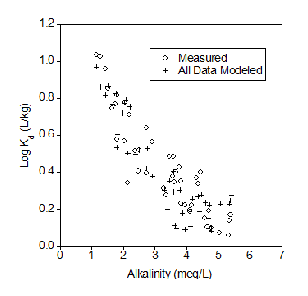
\includegraphics[width=0.5\textwidth, angle = 0]{stoliker}
\caption[Experimentally determined partitioning of U(VI) between 
U-contaminated sediments and artificial groundwater varying in composition 
between that of the Hanford aquifer (high alkalinity) and 
the Columbia River (low alkalinity).  
Partitioning is expressed as the ratio of the U(VI) concentration 
on the sediments (mol/kg sediments) divided by the U(VI) 
concentration in the aqueous phase (mol/L). ]{Experimentally determined partitioning of U(VI) between 
U-contaminated sediments and artificial groundwater varying in composition 
between that of the Hanford aquifer (high alkalinity) and 
the Columbia River (low alkalinity).  
Partitioning is expressed as the ratio of the U(VI) concentration 
on the sediments (mol/kg sediments) divided by the U(VI) 
concentration in the aqueous phase (mol/L). }
% From Stoliker et al. (2011).
\label{fig:stoliker}
\end{figure}

The composition in Table \ref{tab:stoliker}
represents of the composition of U-contaminated groundwater from the Hanford aquifer.  

\begin{itemize}
\item Create a PHREEQC input file that has thermodynamic data for the Ca- and Mg-U(VI)-carbonate complexes.
\end{itemize}

\begin{quote}
{\color{red}SOLUTION\_SPECIES \\
Ca+2 +  UO2+2  +  3CO3-2  =  CaUO2(CO3)3-2 \\
log\_k	27.18 \\
2Ca+2 +  UO2+2  +  3CO3-2  =  Ca2UO2(CO3)3-2 \\
log\_k	30.7 \\
Mg+2 +  UO2+2  +  3CO3-2  =  MgUO2(CO3)3-2 \\
log\_k	26.11 }\\
\end{quote}

\begin{itemize}
\item Enter the groundwater composition in Table \ref{tab:stoliker}. Use the chloride concentration to charge-balance the composition.
\end{itemize}

\begin{table}
\caption{Representative composition of groundwater from Hanford 300 area. Adjust the chloride concentration to charge-balance the solution.}
\begin{center}
\begin{tabular}{l c c }
\hline
Constituent	& Concentration	& Units     \\ \hline
Temperature	& 21	          & $^\circ$C \\
pH	        &     8.11	    &  -        \\
Na	        & 6.8	          & mmol/L    \\
K	          & 0.2	          & mmol/L    \\
Mg	        & 0.4	          & mmol/L    \\
Ca	        & 0.5	          & mmol/L    \\
U(6)	      & 0.001	        & mmol/L    \\
Alkalinity	& 5.00	        & mmol/L    \\
Cl*	        & 1             & mmol/L    \\	
Sulfate	    & 1.4	          & mmol/L    \\ \hline
\end{tabular}
\label{tab:stoliker}
\end{center}
\end{table}
\begin{itemize}
\item Using the Wateq4f database, run a simulation of the groundwater chemistry in Table \ref{tab:stoliker}.
\begin{enumerate}
\item What is the $PCO_2$ ? Recall that the SI for $CO_2(g)$ is the log of the $PCO_2$.
\item What $U(VI)$ aqueous species comprise 99\% of the total dissolved $U(VI)$ ?
\end{enumerate}

\item Next you will simulate changes in chemical composition resulting from transferring the sample into an anaerobic glove chamber that has a $PCO_2$ of 0.05 (5\%). Using the keyword $EQUILIBRIUM\_PHASES n$, allow the sample to equilibrate with the partial pressure of $CO_2$ of 0.05 in the anaerobic chamber. Assume there is an excess of $CO_2$ in the chamber, so that mass transfer of $CO_2$ into or out of the sample does not affect the $PCO_2$ in the chamber.

\begin{quote}
{\color{red}EQUILIBRIUM\_PHASES 5\\ 
CO2(g)  -1.30   1 \\
\# Name of the phase under the PHASES keyword \\
\# in the database or input file. \\
\# -1.30  is the saturation index of the \\ 
\# gas-phase constituent = log of the $PCO_2$ \\
\# 1 is the number of moles of CO2 available \\
\# for transfer into the aqueous solution. \\}
\end{quote}

\item Run the simulation using the Wateq4f database.
\begin{enumerate}
\item Verify that the PCO2 is 0.05.
\item Did $CO_2$ transfer into the aqueous solution or out of the aqueous solution ?
\item item How many moles of $CO_2$ were transferred?
\item How did the $alkalinity$ change?
\item How did the $pH$ and $TCO_2$ change?
\item Was there a significant change in distribution of U(VI) aqueous species?
\item Did the saturation index for calcite change?
\end{enumerate}
\item Now equilibrate the groundwater sample with the atmosphere. Assume that the $PCO_2$ in the atmosphere has a partial pressure of 4.0E-4 atmospheres (logPCO2 = -3.40). Run the simulation using the Wateq4f database.
\begin{enumerate}
\item Verify that the $PCO_2$ is -3.40.
\item Did $CO_2$ transfer into the aqueous solution or out of the aqueous solution ?
\item How many moles of $CO_2$ were transferred ?
\item How did the $alkalinity$ change ?
\item How did the $pH$ and $TCO_2$ change ?
\item Was there a significant change in distribution of $U(VI)$ aqueous species?
\item	Did the saturation index for calcite change ?
\end{enumerate}
\item Re-run the simulation allowing calcite to precipitate if it becomes supersaturated after equilibration with atmosphere.
\begin{enumerate}
\item Verify that the $PCO_2$ is -3.40.
\item Did $CO_2$ transfer into the aqueous solution or out of the aqueous solution?
\item How many moles of $CO_2$ were transferred?
\item How did the $alkalinity$ change ?
\item How did the pH and $TCO_2$ change ?
\item Was there a significant change in distribution of $U(VI)$ aqueous species ?
\item Did the saturation index for calcite change?
\end{enumerate}
\end{itemize}
\section[PHT3D Exercise 1: Transport and mineral reactions]{PHT3D Exercise 1: Transport and mineral reactions}

The present exercise is the first PHT3D application example. 
Building on the experience gained from the first PHREEQC examples, 
it combines a simple one-dimensional flow/mass transport simulation with
mineral precipitation/dissolution reactions.

The case simulated in this exercise was originally presented by
\cite{enges92} for a model verification of their MST1D code
against the CHEMTRNS model by \cite{noor87}. It involves a
one-dimensional model domain in which an aqueous water composition
that is in equilibrium with two minerals, calcite and dolomite, is
successively replaced, i.e., flushed by water of a different
chemical composition, leading to multiple
precipitation - dissolution fronts. Dolomite is not present
initially but is formed temporally.

\subsection[Spatial discretisation and flow problem]{Spatial discretisation and flow problem}

In order to exactly reproduce the discretisation chosen by \cite{enges92}, 
the total length of the model domain must be set to 0.5 $m$ and subdivided 
into 50 grid cells of 0.01 $m$ length. Each of these cells has a width of 1 $m$ and 
also a height of 1 $m$ height. With this discretisation the model
has 50 columns, 1 row and 1 layer. 
The total simulation time is 0.24 days. 
The temporal discretisation (time step length) is set to 0.01 day.

With the selected model dimensions a steady-state flow rate $Q_{well}$ 
of 0.259 $m^3\ d^{-1}$ is required to achieve the pore-velocity of 0.81 $m\
d^{-1}$ (as defined by \cite{enges92}) for a porosity of 0.32. A summary of the
parameters that define the flow field and the non-reactive transport
simulation is given in Table \ref{ex2_flow}.

\begin{table}[b]
\caption{Flow and transport parameters used in PHT3D Exercise 1.}
\begin{center}
\begin{tabular}{lc}
\toprule
 Flow simulation                      &  steady state   \\
 Total simulation time\  $(days)$     &  0.24        \\
 Time step \  $(days)$                         &  0.01           \\
 Grid \ spacing\ $(m)       $         &  0.01           \\
 Model \  length\ $(m)      $         &  0.50           \\
 Pore  \ velocity\ $(m/day) $         &  0.81           \\
 Hydraulic conductivity $(m/day) $    &   1             \\
 Effective Porosity\ $(-)$            &  0.32           \\
 Total Porosity\  $(-)$               &  0.32           \\
 Dispersivity\ $(m)         $         &  0.0067         \\ 
 \bottomrule
\end{tabular}
\label{ex2_flow}
\end{center}
\end{table}

To implement this model setup into ORTI proceed as follows:

\begin{itemize} 

\item In ORTI, create a new model and save it in a new and separate directory
to avoid any mixup of different models and model results.

\item Under {\color{blue}Parameters} $\rightarrow$ {\color{blue}Model} select the {\color{blue}Grid} button and specify the model domain in the dialog that opens up. Use the values as discussed above 
and listed in Table \ref{ex2_flow}.

\item Under {\color{blue}Parameters} $\rightarrow$ select the {\color{blue}Time} button to define the simulation time of 0.24 days under {\color{blue}Total Simulation Time} and the {\color{blue}Step Size} 
to a value of 0.01 day

\item Go to {\color{blue}Spatial Attributes} $\rightarrow$ {\color{blue}MODFLOW} $\rightarrow$ {\color{blue}DIS} $\rightarrow$ {\color{blue}dis.6 Top of Layers (TOP)} and set the top of the model to 1 m. Don't forget to validate the input by clicking the {\color{blue}OK} button.

\item Go to {\color{blue}Spatial Attributes} $\rightarrow$ {\color{blue}MODFLOW} $\rightarrow$ {\color{blue}DIS} $\rightarrow$ {\color{blue}dis.7 Bottom of Layers (BOT)} and set the value to 0 m (the default value).

\item Set the boundary conditions for heads by going to {\color{blue}Spatial Attributes} $\rightarrow$ {\color{blue}MODFLOW} $\rightarrow$ {\color{blue}BAS6} $\rightarrow$ {\color{blue}bas.3 Boundary Conditions} and setting the value to 1 (= active cell) for all cells. After that select {\color{blue}Zone} and use the {\color{blue}Zone Tools} to add a line at the last cell, which represents the downstream boundary. The value of the zone needs to be set to -1 (fixed head). This will define a fixed head boundary, i.e., the hydraulic head at this grid cell will remain at the value that will be defined as initial head. 

\item Set initial hydraulic heads by going to {\color{blue}Spatial Attributes} 
$\rightarrow$ {\color{blue}MODFLOW} $\rightarrow$ {\color{blue}BAS6} 
$\rightarrow$ {\color{blue}bas.5 Initial Heads} and set {\color{blue}one\_value} to 1. 
The initial heads will be used by MODFLOW as initial estimates for solving the flow equations. 
During the solution procedure the correct heads will be computed. 
At locations for which a fixed head boundary condition was defined the heads 
will remain unchanged, as discussed above. 

\item Go to {\color{blue}Spatial Attributes} $\rightarrow$ {\color{blue}MODFLOW} $\rightarrow$ {\color{blue}LPF} $\rightarrow$ {\color{blue}lpf.8} to specify the hydraulic conductivity to 1 $m/day$

\item Go to {\color{blue}Spatial Attributes} $\rightarrow$ {\color{blue}MODFLOW} $\rightarrow$ {\color{blue}WEL} and add a zone {\color{blue}Well} and set the flow rate of the first cell, i.e., the cell representing the inflow end of the model, to 0.259 $m^3/day$.



\end{itemize}

\subsection{Running MODFLOW}

You have now completed to set up the flow model and you are ready to run MODFLOW.
This step will provide PHT3D with the flow field that is used to compute advective - dispersive
transport of mobile species/components:

\begin{itemize}

\item Under {\color{blue}Parameters} $\rightarrow$ {\color{blue}Flow} use the {\color{blue}Write Button} to write all the input files required to run MODFLOW

\item Under {\color{blue}Parameters} $\rightarrow$ {\color{blue}Flow} use the 
{\color{blue}Red Arrow} button to start the MODFLOW simulation

\end{itemize}

During the execution of MODFLOW a number of output files are created, including the specific file {\color{red} \textbf{mt3d.flo}}, which contains the flow vectors of each cell for each time step in the simulation. This file is required for the subsequent PHT3D simulation(s) and PHT3D will not run
until the file {\color{red} \textbf{mt3d.flo}} exists. If changes are made to the MODFLOW 
input parameters MODFLOW needs to be rerun such that the file {\color{red} \textbf{mt3d.flo}} is updated.

\subsection[Data input for solute transport]{Data input for solute transport}

For the simulation of solute transport of the mobile components you need to specify the model parameters that control advective and dispersive transport. It is assumed that the parameters that define the physical transport of the chemicals are the same for every species/component:

\begin{itemize}

\item Go to {\color{blue}Parameters} $\rightarrow$ {\color{blue}Transport} and select the {\color{blue}Parameter} button

\item In the dialog box that subsequently appears, select {\color{blue}ADV} and the 
{\color{blue}3rd-order TVD Scheme (ULTIMATE)} as the Solution Scheme and click {\color{blue}OK}.

\item Select {\color{blue}Spatial Attributes} $\rightarrow$ {\color{blue}MT3DMS} $\rightarrow$ {\color{blue}DSP}, enter a longitudinal dispersivity value of 0.0067 m. and click {\color{blue}ok}

\item Leave the values for the dispersivity ratios and diffusion coefficients as they are and click {\color{blue}OK}.

\item Go to {\color{blue}Spatial Attributes} $\rightarrow$ 
{\color{blue}MT3DMS} $\rightarrow$ {\color{blue}BTN} $\rightarrow$ (\color{blue}btn.11)
and specify the effective porosity to be 0.32.

\end{itemize}



\subsection[PHT3D reaction definition]{PHT3D reaction definition}

We continue now with the setup of the reactive transport model. In some cases
the next step would be to prepare a problem-specific reaction module.   
However, for simpler problems such as the one in this exercise and many others
that only include equilibrium reactions, this is not the case. 
All of the aqueous species, components and minerals needed to
simulate this LEA-based reactive transport problem are already
included in the original PHREEQC-2 database. 
This means that we don't have to define our own set of equilibrium reactions 
but we can simply use a PHT3D database file that is equivalent to
the original PHREEQC-2 database. 
To specify this and to incorporate the correct reaction database, 
proceed as follows:

\begin{itemize}

\item Copy the database file that is going to be used for the PHT3D simulation
into the folder that contains all files for this exercise and name the file {\color{red} \textbf{pht3d\_datab.dat}}.

\item Go to {\color{blue}Parameters} $\rightarrow$ {\color{blue}Chemistry} and select the
{\color{blue}Import database} button. ORTI will then read and interpret 
the PHT3D database file.

\item Then click on the {\color{blue}Chemical Reaction} button. This will open up a new dialog box

\item Within the new dialog box go to the {\color{blue}Solution} Tab and 
select the aqueous components that you want to 
include in the model. 
In this exercise the simulation needs to include C(4), Ca, Cl, Mg, pe and pH.

\item Then click the {\color{blue}Phases} Tab and select (i.e., activate) the two 
minerals Calcite and Dolomite.

\end{itemize}

These steps are the only steps needed to define the set of chemical reactions 
that will be considered in the PHT3D simulation. 
From this information ORTI will create the interface file that controls the communication
between the MT3DMS part and the PHREEQC-2 part of the PHT3D simulator. 
This file, {\color{red} \textbf{pht3d\_ph.dat}}, contains the records which define that the 
reaction network contains 6 equilibrium aqueous components 
(including pH and pe) and two equilibrium minerals. 
The order in which the components are listed determines which species number will 
be allocated to each entity included in the simulation. 
For each of the first {\color{red} \textbf{MCOMP}}-2 (C(4)), Ca, Mg, Cl) 
of the {\color{red} \textbf{NCOMP}} components advective-dispersive transport steps will 
be simulated by the appropriate MT3DMS routines. 
For component numbers {\color{red} \textbf{MCOMP}}-1 (pH) and 
{\color{red} \textbf{MCOMP}} (pe) no transport step is carried out. 
The entities {\color{red} \textbf{MCOMP}} + 1, ... ,{\color{red} \textbf{NCOMP}} (here Calcite
and Dolomite) are immobile and no transport simulation will be carried out for them.

\subsection[Initial and inflow concentrations]{Initial and inflow concentrations}

The next step in setting up this problem is to specify the initial concentrations
that define the hydrogeochemistry of the aquifer at the start of the simulation (Time = 0).
The information provided here will be translated by ORTI into the 
the basic transport package file, which is called  {\color{red} \textbf{pht3dbtn.dat}}
in PHT3D. The initial concentrations that need to be entered into ORTI,
as defined in the paper by \cite{enges92}, are listed in
Table \ref{ex2_caqu} (for aqueous components) and in Table \ref{ex2_cmin} (for minerals).
\\
\ \\
\textbf{Note, that aqueous concentrations are always defined in units of $mol\ l^{-1}$.
In contrast, the unit for the initial concentrations of minerals
is NOT mass per volume of water, i.e., $mol\ l^{-1}$,
but is defined as mass per bulk volume, i.e., $mol\ l^{-1}_{volume}$}. \\
\ \\
\cite{enges92} defined their mineral concentrations as mass per
mass of soil, i.e., $mol\ kg_{soil}^{-1}$ and provided the bulk
density (1800 $kg\ m^{-3}$) of the soil. Therefore, their initial
concentrations for calcite of 2.176 $\times$ $10^{-5}$ $mol\
kg_{soil}^{-1}$ translates to 3.906 $\times$ $10^{-5}$ $mol\
l^{-1}_{volume}$, which needs to be used in PHT3D.
\par If a simulation problem, like the one we are 
simulating here, is a pure equilibrium problem, it should
be warranted that the initial water composition is in chemical equilibrium
and the aqueous solution is charge-balanced. 
If the aqueous solution is not in equilibrium, equilibrium conditions
will be adjusted within the first reaction step at the end of the
first time step. This can cause an undesired change, for example,
of the solution pH or the dissolution/precipitation of minerals. 
To avoid this it is recommended to study and
charge-balance the aqueous solution with PHREEQC before entering
the data into ORTI.

\begin{table}[hb]
\caption{Aqueous concentrations used in PHT3D Exercise 1.}
\begin{center}
\begin{tabular}{l c c}
\hline
 Aqueous component       & $C_{init}$ & $C_{inflow}$      \\
                & $(mol\ l^{-1}_w)$   & $(mol\ l^{-1}_w)$      \\ \hline
 pH             &   9.91    &  7.0            \\
 pe             &   4.0     &  4.0            \\
 C(4)           &  1.23 $\times$ $10^{-4}$ &   $  0.0  $              \\
 Ca             &  1.23 $\times$ $10^{-4}$ &   $  0.0  $               \\
 Mg             &     0.0                  & 1.0 $\times$ $10^{-3}$   \\
 Cl             &     0.0                  & 2.0 $\times$ $10^{-3}$   \\ \hline
\end{tabular}
\label{ex2_caqu}
\end{center}
\end{table}

\begin{table}[hb]
\caption{Mineral concentrations used in PHT3D Exercise 1.}
\begin{center}
\begin{tabular}{ l c }
\hline
 Mineral        & $C_{init}$  \\
                  & $(mol\ l^{-1}_{v})$  \\ \hline
 Calcite \   $(CaCO_3)  $  & 3.906 $\times$ $10^{-5}$  \\
 Dolomite  \ $(CaMg(CO_3)_2) $  &   0.0             \\ \hline
\end{tabular}
\label{ex2_cmin}
\end{center}
\end{table}


There are various ways and types of boundary conditions to define the hydrochemical
composition of water that is entering the model domain during a simulation.
In the present case the inlet (inflow) water composition is defined by providing the 
aqueous component concentrations for the injection well located at the first cell. The inlet water contains 0.001 $mol\ l^{-1}$ of Mg and 0.002 $mol\ l^{-1}$ of Cl. In contrast to the initial water composition, no C(4) and no Ca is contained in the inflow water. 
You can enter these values (see also Table \ref{ex2_caqu}) into ORTI as follows: \\

To define both the initial and inflow concentrations 
you will enter the chemical composition of the respective aqueous solutions. 
In this exercise the background contains water that is in chemical equilibrium 
with the mineral $Calcite$. 
The composition of the initial water needs to be entered under the 
{\color{blue}Solutions} Tab in the {\color{blue}Background} column.
On the other hand the initial mineral composition must be entered 
under the {\color{blue}Phase} Tab that contains the input values 
for the saturation index (SI) and the initial concentration (Backgr\_SI and Backgr\_Mol, respectively).
Leave the SI at the default value of 0, as would be the case for most typical model applications.
The inflow water composition will be defined 
in the {\color{blue}Solution 1} column under the {\color{blue}Solutions} Tab.


To additionally define that the inflow composition is used at the correct location
(i.e., the inflow boundary) we need to select {\color{blue}Spatial Attributes} $\rightarrow$ 
{\color{blue}PHT3D} $\rightarrow$ {\color{blue}PH} $\rightarrow$ {\color{blue}ph.4 Source \/ Sink}
and define a zone (point) in the same zone as the well at the inflow boundary 
and allocate a {\color{blue}Zone Value} 
of 1. This induces that the previously defined concentrations 
for Solution 1 (as defined in the {\color{blue}Solutions} Tab) will be used to specify
the concentrations in the water that enters the column. 



\subsection[Running PHT3D]{Running PHT3D}

To run PHT3D, proceed as earlier in the exercise when executing MODFLOW:

\begin{itemize}

\item Go to {\color{blue}Parameters} $\rightarrow$ {\color{blue} Chemistry} and use 
the {\color{blue}Write Button} to write all the input files required to run PHT3D

\item Then go to {\color{blue}Parameters} $\rightarrow$ {\color{blue}Chemistry} and use the {\color{blue}Plume Button} to start PHT3D.

\end{itemize}


\subsection[Visualization of simulation results]{Visualization of simulation results}

To visualise the simulation results and to compare them with the results 
we need to extract the simulated concentrations in the form of concentration profiles 
for the end of the simulation time. This can be achieved by creating a so-called observation zone. 
This option can be used to display the results graphically but also to export the results and save them in newly created data files.  

\begin{itemize}

\item Select {\color{blue}Spatial Attributes} $\rightarrow$ {\color{blue}Observation} $\rightarrow$ {\color{blue}OBS} $\rightarrow$ {\color{blue}obs.1} $\rightarrow$ {\color{blue}Zone}
and create a zone as a horizontal line that maybe named $line1$. 
No additional input is needed here.

\item In the {\color{blue}Results Panel} select the final time step of the simulation
by going to {\color{blue}Results} $\rightarrow$ {\color{blue}Aquifer} 
$\rightarrow$ {\color{blue}Tstep} and selecting {\color{blue}0.24} days

\item In the {\color{blue}Results} sub-panel select one of the specific species that you want to visualise
by going to {\color{blue}Results} $\rightarrow$ {\color{blue}Chemistry} 
$\rightarrow$ {\color{blue}Species} and selecting, for example, {\color{blue}Ca}. 

\item Then go to {\color{blue}Results} $\rightarrow$ {\color{blue}Observation} and select the 
visualisation type {\color{blue}Profile}. Then select the {\color{blue}Profile} option

\item in the following dialog you can either select a single or multiple species. 
For pure visualisation the selection of multiple species makes only sense for all those 
species which prevail within the same concentration range. 
However, in this exercise we want to export the data for multiple species and 
therefore we select all of the simulated species 

\item Once the species are selected a new dialog will open. This new dialogue allows to make a selection among several types of concentration averaging techniques. 
In the present case simply select the default option, i.e., {\color{blue}Value}

\item Now a plot should appear that shows the simulated concentrations of all selected species 
along the previously defined $line1$, i.e., concentration profiles along the column should show up

\item You can now use the {\color{blue}Export} button to export the simulated values into a text file.
If you export $Ca$, $Mg$, $Cl$, $Calcite$ and $Dolomite$ you can copy/paste the results into the pre-prepared excel file and compare your model results with those obtained by \cite{enges92}

\end{itemize}

\subsection[Comparison of simulation results]{Comparison of simulation results}

If all steps of the model definition were performed correctly
the results should agree closely with those otained by \cite{enges92},  
as illustrated in Figure \ref{pht3d_mst1d}.
Generally the simulated concentrations, including the positions of the mineral 
fronts agree very well. However, the PHT3D-simulated pH near the inflow end of 
the model domain lies slightly above the pH simulated by MST1D.

\begin{figure}[ht]
\centering
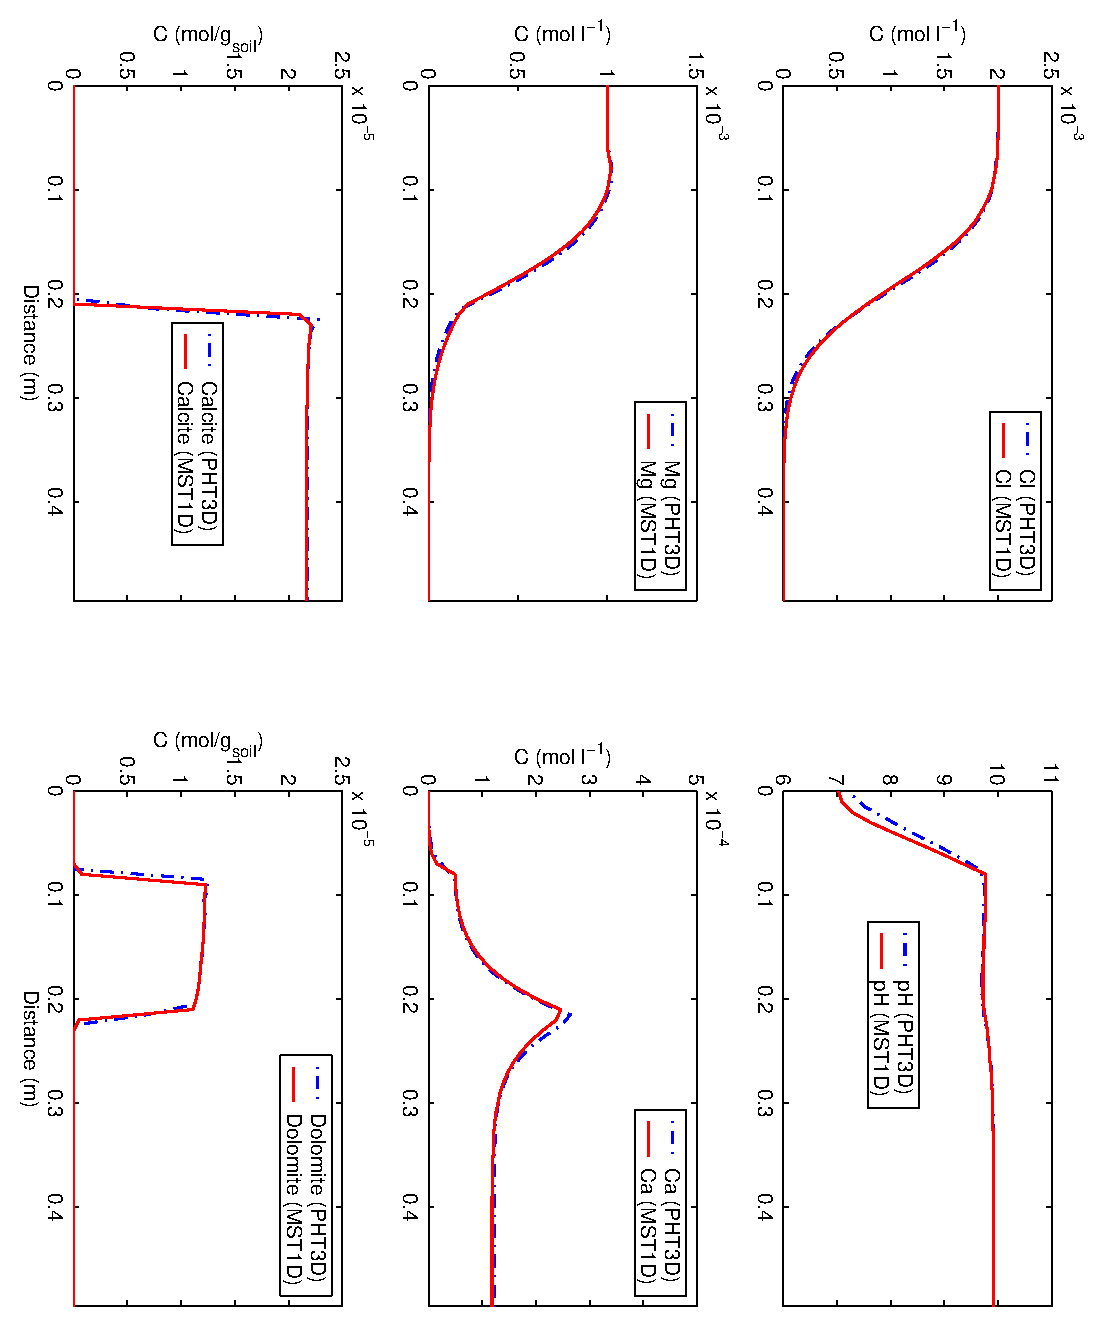
\includegraphics[width=80mm,angle=90]{ex2.eps}
\caption[Simulation results for PHT3D and MST1D: Aqueous and
mineral concentrations after 21000 s.] {Simulation results for
PHT3D and MST1D: Aqueous and mineral concentrations after 21000 s.}
\label{pht3d_mst1d}
\end{figure}



\section[PHT3D Exercise 2: Mineral buffering Acid rain and mineral bufferin]{PHT3D Exercise 2: Acid rain and mineral buffering}

%\subsection{Introduction}

This exercise is a simple two-dimensional simulation problem that involves mineral dissolution reactions. 
Most importantly this example illustrates the concept of mineral buffering reactions that can occur 
in response to acidic groundwater recharge entering an aquifer. 
The problem is set up as a vertical transect representing a small catchment with groundwater being the only driver for groundwater flow. We will study the evolution of the water quality that discharges to the river over a 50-year period (18250 days). This will mimic, although in a crude way, the response to the atmospheric sulfur deposition that has occurred (and in some places still occurs) in conjunction with air pollution from industrial emissions.
The increased sulphur input was associated with a decline of the pH within the rain and the recharge water.
The increased acidity of the recharge water can cause the enhanced dissolution of selected minerals, which act as pH buffers. The dissolution of these minerals will raise the pH of the groundwater until they are depleted. 
With the exercise we compare different scenarios and show the influence of the initial concentration of the buffering mineral on the longevity of the buffering process.

\subsection[Spatial discretisation and flow problem]{Spatial discretisation and flow problem}

The problem is set up as a simple two-dimensional flow and transport problem with dimensions and properties as defined in Table \ref{franken_flow}. To construct the MODFLOW model that underlies the transport problem proceed as follows:

%\begin{figure}[b]
%\centering
%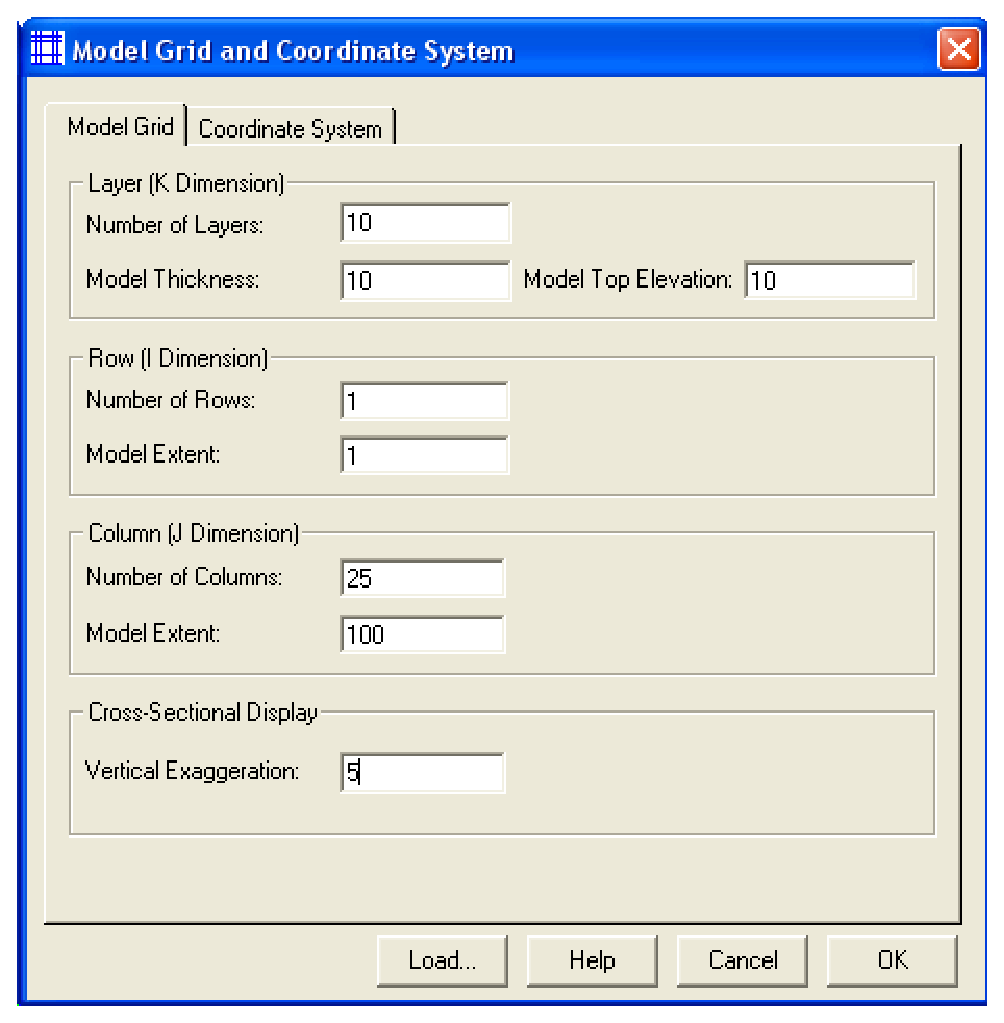
\includegraphics[width=80mm]{walter.eps}
%\caption[Initial definition of the model grid for PHT3D Exercise 2]{Initial definition of the model grid for PHT3D %Exercise 2}
%\label{fig:mesh_walter}
%\end{figure}


\begin{itemize}

\item In ORTI, create a new model and save it in a new, separate directory.

\item Under {\color{blue}Parameters} $\rightarrow$ {\color{blue}Model} select the {\color{blue}Model} button and specify the attributes of the new model. Select the values {\color{blue}Xsection} for {\color{blue}Dimension}, {\color{blue}unconfined} for {\color{blue}Type} 
and {\color{blue}MODFLOW series} for {\color{blue}Group} 

\item Under {\color{blue}Parameters} $\rightarrow$ {\color{blue}Model} select the {\color{blue}Grid} button and specify the details of the model domain and the spatial discretisation in the dialog that opens up. Define a vertical transect that is 2000m long and 20m thick. The model domain
may be discretised into grid cells of 40m length and 1m height. Note, that the 
model discretisation can be easily changed again later. 

\item Select {\color{blue}Parameters} and select the {\color{blue}Time} button.
Set the {\color{blue}Total Simulation Time} to 18250 days and select a time {\color{blue}Step size}
of 182.5 days. 

\item Go to {\color{blue}Spatial Attributes} $\rightarrow$ {\color{blue}MODFLOW} $\rightarrow$ {\color{blue}LPF} $\rightarrow$ {\color{blue}lpf.8} to specify the horizontal hydraulic conductivity to 20 $m/day$

\item Go to {\color{blue}Spatial Attributes} $\rightarrow$ {\color{blue}MODFLOW} $\rightarrow$ {\color{blue}LPF} $\rightarrow$ {\color{blue}lpf.9} to specify the vertical hydraulic conductivity to 1 $m/day$

\item Go to {\color{blue}Spatial Attributes} $\rightarrow$ {\color{blue}MT3DMS} $\rightarrow$ {\color{blue}BTN} $\rightarrow$ {\color{blue}btn.11} and specify the effective porosity to be 0.25.


\item Implement a hydraulic boundary condition that represents the river at the down stream end of this synthetic catchment by defining a specified head boundary at the downstream side of the model. First, define the type of boundary condition by going to {\color{blue}Spatial Attributes} $\rightarrow$ {\color{blue}MODFLOW} $\rightarrow$ {\color{blue}BAS6} $\rightarrow$ {\color{blue}bas.3 Boundary Conditions} and setting the value to 1 (= active cell) for all cells. After that select {\color{blue}Zone} and use the {\color{blue}Zone Tools} to draw a short line near the effluent end. Choose an elevation of z = 8.5 m for the line and draw it from x = 1m to x = 20m. 
The value for the line (=zone) needs to be set to -1. Use, for example,
$river\_bc$ as {\color{blue}Zone Names}. You will see the selected name displayed near 
the location of the line.
  
By setting the boundary condition type to -1 the hydraulic head at the grid cells 
near the defined line will remain unchanged
over the entire simulation period, i.e., it will remain at the value that corresponds to the elevation of
the river water level. In the next step the initial heads need to be defined. 

\item First the define the global initial hydraulic head for the entire domain (Background value) by going to {\color{blue}Spatial Attributes} $\rightarrow$ {\color{blue}MODFLOW} $\rightarrow$ {\color{blue}BAS6} $\rightarrow$ {\color{blue}bas.6 Initial Heads} and set the
 {\color{blue}Backg.} value to 20m. Then press {\color{blue}'OK'} to confirm the value.  

\item Define the initial hydraulic head at the location of the river by going to {\color{blue}Spatial Attributes} $\rightarrow$ {\color{blue}MODFLOW} $\rightarrow$ {\color{blue}BAS6} $\rightarrow$ {\color{blue}bas.6 Initial Heads}.
Select {\color{blue}Zone} and use the {\color{blue}Zone Tools} to draw again a short line near the effluent end. Choose an elevation of z = 8.5 m for the line and draw it from x = 1m to x = 20m. 
Note, that you can edit the coordinates manually after you have completed the drawing.
The value for the line (=zone) needs to be set to 8.5. Use, for example,
$river\_head$ as {\color{blue}Zone Names}. You will see the selected name and the selected value
displayed near the location of the line.
  

To define the groundwater recharge for this model you will first need to activate the recharge package,
as it is not automatically activated.
This can be done by going to {\color{blue}Add-in} $\rightarrow$ {\color{blue}MODFLOW modules} 
and ticking the box {\color{blue}RCH}. Then tick {\color{blue}OK}.
You will see that you can now go to {\color{blue}Spatial Attributes} $\rightarrow$ {\color{blue}MODFLOW} $\rightarrow$ {\color{blue}RCH} $\rightarrow$ {\color{blue}rch.2 Recharge value} and set the {\color{blue}Backg.} value to 0.001m, corresponding to an annual groundwater recharge of 365mm per year.
Then press {\color{blue}'OK'} to confirm the value. 



\end{itemize}

\begin{table}[t]
\caption{Flow and transport parameters for the simulation.}
\begin{center}
\begin{tabular}{lc} 
\toprule
Flow simulation                     & steady state \\
Total simulation period\ $ (days)      $         &  18250            \\
Time step length\ $ (days)      $         &  182.5            \\
Model \  length\ $ (m)      $         &  2000            \\
Model \  thickness\ $(m)$                        &  20            \\
Grid \ spacing\ $\Delta x $ $(m)$                &    40            \\
Grid \ spacing\ $\Delta z $ $(m)$                &    1            \\
Porosity\     $            $         &  0.25           \\
Horizontal hydraulic conductivity\ $(m/day)$               &  20         \\ 
Vertical   hydraulic conductivity\ $(m/day)$               &  1         \\ 
Piezometric head downstream boundary (River)\ $(m)        $         &  8.5           \\ 
Longitudinal dispersivity\ $(m)         $         &  2.5          \\ 
Transverse  vertical dispersivity\ $(m)         $         &  0.025          \\ 
\bottomrule
\end{tabular}
\label{franken_flow}
\end{center}
\end{table}

\subsection{Running MODFLOW}

You have now completed to set up the flow model and you are ready to run MODFLOW.

\begin{itemize}

\item Under {\color{blue}Parameters} $\rightarrow$ {\color{blue}Flow} use the {\color{blue}Write Button} to write all the input files required to run MODFLOW

\item Under {\color{blue}Parameters} $\rightarrow$ {\color{blue}Flow} use the 
{\color{blue}Red Arrow} button to start the MODFLOW simulation

\item Check the simulated head contours and assess whether the results are plausible.

\item Try, for example to set the head contours manually at 0.25m intervals, starting from 8.5m.

% Olivier, maye we can practise the use of some more iPHT3D output features 

\end{itemize}

% Here we had a non-reactive model step in the pmwin version of the tutorial

\subsection[Data input for solute transport properties]{Data input for solute transport properties}

For the simulation of the solute transport of the mobile components the model parameters that control advective and dispersive transport need to be entered. 

\begin{itemize}

\item Go to {\color{blue}Parameters} $\rightarrow$ {\color{blue}Transport} and select the {\color{blue}Parameter} button

\item In the dialog box that subsequently appears, select {\color{blue}ADV} and select under {\color{blue}adv.1 Solver Parameters} the {\color{blue}MMOC} as the Solution Scheme. Leave the default parameters and click {\color{blue}ok}.

\item Select {\color{blue}Spatial Attributes} $\rightarrow$ {\color{blue}MT3DMS} $\rightarrow$ {\color{blue}DSP}, enter a longitudinal dispersivity value of 5 m. and click {\color{blue}OK}

\item Select {\color{blue}Spatial Attributes} $\rightarrow$ {\color{blue}MT3DMS} $\rightarrow$ {\color{blue}DSP}, and specify that the ratio between transverse vertical dispersivity and the longitudinal dispersivity is 0.01.
This will define that the actual value is 0.05 m (= 50mm). 


\end{itemize}

\subsection[Data input for reactive transport]{Data input for reactive transport}

In the following step we will now activate the geochemical reaction network and define the various water and mineral compositions that will play a role in this simulation problem. The initial and the groundwater recharge water composition that will be employed in this example are shown in Table \ref{franken_caqu}. 

\begin{table}
\caption{Aqueous concentrations used in acid groundwater recharge exercise}
\begin{center}
\begin{tabular}{l c c}
\hline
Aqueous  component        & $C_{init}$ & $C_{recharge}$      \\
                  & $(mol\ l^{-1}_w)$   & $(mol\ l^{-1}_w)$      \\ \hline
pH              &   7.00    &  4.18           \\
pe              &   4.00    &  4.00           \\
Al              &  1.538 $\times$ $10^{-5}$ & 0   \\
C(4)            &  6.041 $\times$ $10^{-5}$ & 5.736 $\times$ $10^{-5}$   \\
C(-4)           &  0                       &     0                     \\
Cl              &  9.345 $\times$ $10^{-4}$ & 7.335 $\times$ $10^{-5}$   \\
Na              &  1.000 $\times$ $10^{-3}$ & 2.827 $\times$ $10^{-5}$   \\
S(6)            &  1.000 $\times$ $10^{-6}$ & 1.072 $\times$ $10^{-5}$   \\
S(-2)           &     0             &     0               \\
Si              &  1.107 $\times$ $10^{-4}$ & 0  \\ \hline
\end{tabular}
\label{franken_caqu}
\end{center}
\end{table}


\begin{itemize}

\item Copy the database file that is going to be used for the PHT3D simulation
into the folder that contains all files for this exercise and name the file {\color{red} \textbf{pht3d\_datab.dat}}. You can use the standard PHREEQC database for this example.

\item Go to {\color{blue}Parameters} $\rightarrow$ {\color{blue}Chemistry} and select the
{\color{blue}Import database} button. ORTI will then read and interpret 
the PHT3D database file.

\item In this next step we define all initial concentrations of all aqueous components
also the concentrations of the acidic groundwater recharge. The composition of the ambient water (initial water composition at the start of the simulation) 
needs to be entered under the {\color{blue}Solutions} Tab in the {\color{blue}Background} column.
Activate all relevant species by ticking the appropriate boxes for 
$pH$, $pe$,  $Al$, $C(4)$,  $C(-4)$, $Cl$, $Na$, $O(0)$, $S(6)$, $S(-2)$,and $Si$
and enter the concentrations that are provided in the Table. In the next step define the acid 
recharge water composition by entering the values from the Table in the {\color{blue}Solution 1} column 
under the {\color{blue}Solutions} Tab.  

\item The {\color{blue}Background} water composition will automatically be used to define the 
initial concentrations.

\item The allocation of {\color{blue}Solution 1} groundwater water recharge composition can be
done by selecting {\color{blue}Spatial Attributes} $\rightarrow$ {\color{blue}PHT3D} $\rightarrow$ {\color{blue} ph.5Recharge} and set {\color{blue}Backg.} to 1.  

\end{itemize}

\subsection[Running PHT3D]{Running PHT3D}

In this first step we will now run PHT3D without invoking any mineral reactions. This means that all temporal and spatial concentration changes of the aqueous components that occur over the simulation period are solely a function of advective-dispersive transport. This provides the basis for subsequently studying the impact of mineral reactions.    

\begin{itemize}

\item Go to {\color{blue}Parameters} $\rightarrow$ {\color{blue} Chemistry} and use 
the {\color{blue}Write Button} to write all the input files required to run PHT3D

\item Then go to {\color{blue}Parameters} $\rightarrow$ {\color{blue}Chemistry} and use the {\color{blue}Plume Button} to start PHT3D.

\end{itemize}

\subsection[Visualisation of results]{Visualisation of results}

After the end of the simulation visualise the results in various ways.

\begin{itemize}

\item Obtain a contour plot by navigating in the {\color{blue} Results} panel of ORTI.
Select a specific timestep and a species for which you want to see your results.
For example to see the pH contours after 10 years select {\color{blue}Results} $\rightarrow$ {\color{blue}Aquifer} 
$\rightarrow$ {\color{blue}Tstep} and select {\color{blue}3650} and then go to   
{\color{blue}Results} $\rightarrow$ {\color{blue}Chemistry} 
$\rightarrow$ {\color{blue}Species} and select {\color{blue}pH}.  
You can easily move forward and backward in time by clicking {\color{blue}Tstep} once more and then
using your keyboard arrows to move forward or backward.

\item Plot breakthrough curves at the river discharge point to illustrate how the quality of the
water discharging from the groundwater to the river changes over time.
First, define the location for which you want to plot breakthrough curves by
going to {\color{blue}Spatial Attributes} $\rightarrow$ {\color{blue}Observation} $\rightarrow$ {\color{blue}OBS} $\rightarrow$ {\color{blue}obs.1} $\rightarrow$ {\color{blue}Zone}
and use your mouse to position the cursor and clicking at the location
where you wan to create an observation point. In the dialog that comes up name the zone $BTC1$. 
No specific input is required for the {\color{blue}Zone Value} field.
The coordinates of the location selected by the mouse click can be modified, if required.

\item Alternatively you can visualise results with PHT3DPlot. 

\item What changes occur to the chloride concentrations and what does this mean ?

\item How much does pH decrease over the duration of the simulation ? 

\item Save the simulated breakthrough curves for pH, Si and Al so you can later directly 
plot and compare these results together with the results from your next model variants.  
 
\end{itemize}



\subsection[Role of mineral reactions]{Role of mineral reactions}

\begin{itemize}

\item Let's first study the effect of including $Quartz$ in this simulation. 
This can be done under the {\color{blue}Phase} Tab. The input allows to activate mineral phases 
and to define values for the saturation index (SI) to which the mineral should be equilibrated (typically 0).
and the initial concentration (Backgr\_SI and Backgr\_Mol, respectively.
Leave the Backgr\_SI at the default value of 0 and define a background concentration Backgr\_Mol of 1 mol/L\_bulk. 

\item Now rerun PHT3D and inspect again the breakthrough curves for pH, Si and Al.

\item How can you interpret these results ?  

\end{itemize}

Now we will inspect the impact of $Al(OH)_3$ on the composition of the discharging groundwater.

\begin{itemize}

\item Add initially a relatively small initial concentration such as 1 $\times$ $10^{-4}$ mol/L\_bulk 
of $Al(OH)_3$, rerun the model and save again the breakthrough concentrations that you obtained for the observation point at the river.

\item Increase the initial concentration to a value such as 1 $\times$ $10^{-2}$ mol/L\_bulk 
of $Al(OH)_3$, rerun the model and save again the breakthrough concentrations that you obtained for the observation point at the river.

\item Make comparative plots for pH and Al for your different model variants. 

\end{itemize}







\section[PHT3D Exercise 3: Precipitation/dissolution fronts in acid mine drainage]{PHT3D Exercise 3: Precipitation/dissolution fronts in acid mine drainage}

%\subsection{Introduction}

This exercise is another simulation problem that involves mineral dissolution and precipitation reactions as the principle geochemical reactions. Compared to the previous 
exercise it is somewhat more complicated as it contains significantly more 
aqueous components and mineral reactions.
It was first presented by \cite{walt94a} and later also used as a benchmark problem by \cite{gmt3d}. In contrast to the previous exercise this case includes now also redox reactions. 
The simulations demonstrate the typical hydrogeochemical changes that occur 
when acidic mine tailings leach into an anaerobic carbonate aquifer. 
Aqueous complexation and dissolution/precipitation are all considered as equilibrium reactions. 
If the original reaction network defined by \cite{walt94a} is used, the simulation 
includes 17 aqueous components, 15 of which are transported, 54 aqueous species and six minerals. 

\subsection[Spatial discretisation and flow problem]{Spatial discretisation and flow problem}

The problem is set up as a simple two-dimensional flow and transport problem with dimensions and properties as defined in \ref{ex3_flow}. To construct the MODFLOW model that underlies the transport problem proceed as follows:

%\begin{figure}[b]
%\centering
%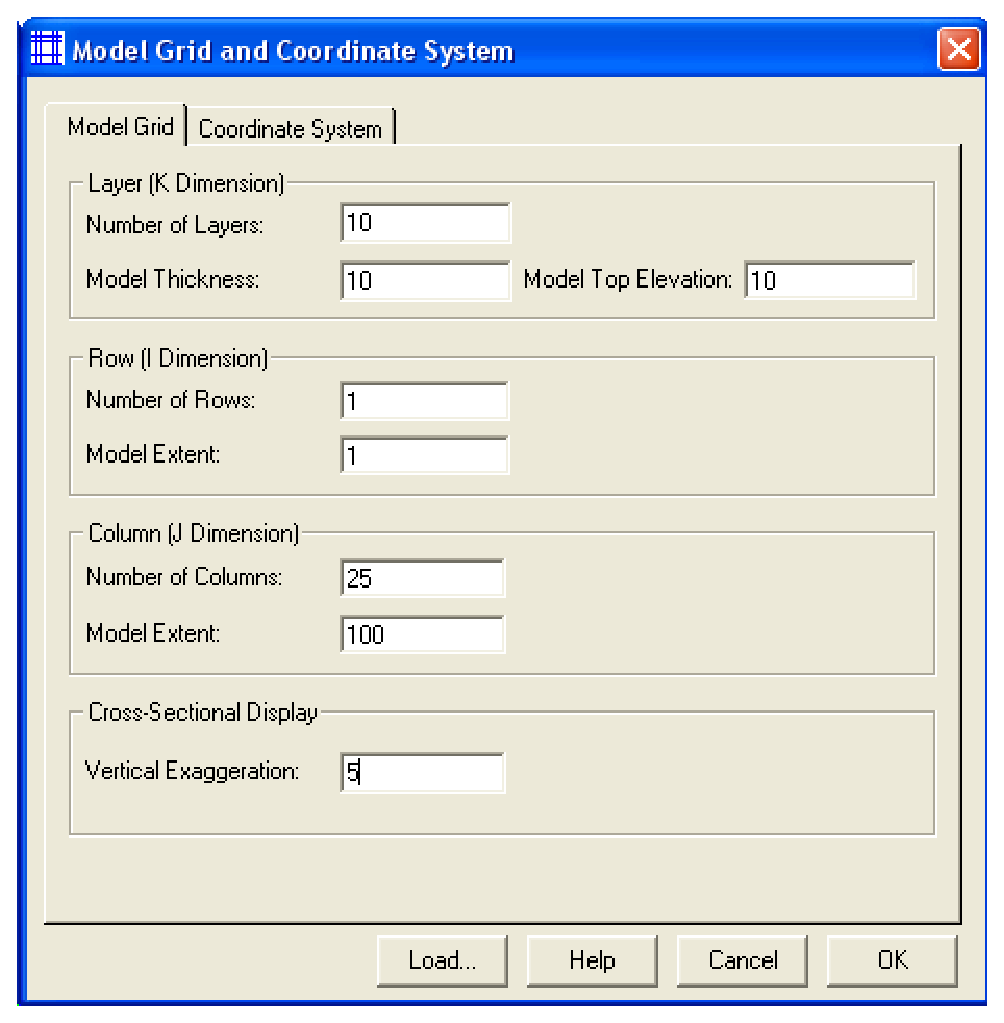
\includegraphics[width=80mm]{walter.eps}
%\caption[Initial definition of the model grid for PHT3D Exercise 2]{Initial definition of the model grid for PHT3D %Exercise 2}
%\label{fig:mesh_walter}
%\end{figure}


\begin{itemize}

\item In ORTI, create a new model and save it again in a new, separate directory.

\item Under {\color{blue}Parameters} $\rightarrow$ {\color{blue}Model} select the {\color{blue}Model} button and specify the attributes of the new model. Select the values {\color{blue}Xsection} for {\color{blue}Dimension}, {\color{blue}Confined} for {\color{blue}Type} 
and {\color{blue}MODFLOW Family} for {\color{blue}Group} 

\item Under {\color{blue}Parameters} $\rightarrow$ {\color{blue}Model} select the {\color{blue}Grid} button and specify the details of the model domain and the spatial discretisation in the dialog that opens up. Define a vertical transect that is 100m long and 10m thick. The model domain
may be discretised into grid cells of 4m length and 1m height. Note, that the 
model discretisation can be easily changed again later. 

\item Select {\color{blue}Parameters} and select the {\color{blue}Time} button.
Set the {\color{blue}Total Simulation Time} to 2000 days and select a time {\color{blue}Step size}
of 20 days. 

\item Go to {\color{blue}Spatial Attributes} $\rightarrow$ {\color{blue}MODFLOW} $\rightarrow$ {\color{blue}LPF} $\rightarrow$ {\color{blue}lpf.8} to specify the hydraulic conductivity to 1 $m/day$

\item Go to {\color{blue}Spatial Attributes} $\rightarrow$ {\color{blue}MODFLOW} $\rightarrow$ {\color{blue}LPF} $\rightarrow$ {\color{blue}lpf.9} to specify the vertical hydraulic conductivity to 1 $m/day$

\item Go to {\color{blue}Spatial Attributes} $\rightarrow$ {\color{blue}MT3DMS} $\rightarrow$ {\color{blue}BTN} $\rightarrow$ {\color{blue}btn.11} and specify the effective porosity to be 0.35.


\item Implement hydraulic boundary conditions by defining the hydraulic heads at the upstream and the downstream boundary of the model. First, define the type of boundary condition by going to {\color{blue}Spatial Attributes} $\rightarrow$ {\color{blue}MODFLOW} $\rightarrow$ {\color{blue}BAS6} $\rightarrow$ {\color{blue}bas.3 Boundary Conditions} and setting the value to 1 (= active cell) for all cells. After that select {\color{blue}Zone} and use the {\color{blue}Zone Tools} to add one line at the inflow end of the model and one line at the effluent end. 
In both cases the lines need to extend over the whole depth of the aquifer. 
The value for both lines (=zones) needs to be set to -1. Use, for example,
$bc\_up$ and $bc\_down$ as {\color{blue}Zone Names}. You will see the selected names displayed near 
the location of the lines.
  
This will define the type of boundary condition to a fixed head boundary 
at the inflow and outflow model boundaries.
The hydraulic head at these grid cells will therefore remain unchanged
over the whole simulation period. It will remain at the same values that we will now define as initial heads.  

\item Set initial hydraulic heads by going to {\color{blue}Spatial Attributes} $\rightarrow$ {\color{blue}MODFLOW} $\rightarrow$ {\color{blue}BAS6} $\rightarrow$ {\color{blue}bas.6 Initial Heads} and set {\color{blue}one\_value} 
to 10, corresponding to a head of 10m. Then press {\color{blue}'OK'} to confirm the value. In addition
define a zone (line) at the upstream end of the model domain (where you also defined that the type of 
boundary condition is -1) and allocate a hydraulic head of 12m over the entire depth of the aquifer. 

% Maybe lets not use recharge here to save time
%\item Add a value for recharge by selecting Models $\rightarrow$ MODFLOW $\rightarrow$ Flow 
% Packages $\rightarrow$ Recharge $\rightarrow$ Reset Matrix and change the value for the Recharge % flux to 0.001 m/d (365 mm/year) and click ok. 

\end{itemize}

\begin{table}[t]
\caption{Flow and transport parameters for the simulation.}
\begin{center}
\begin{tabular}{lc} 
\toprule
Flow simulation                     & steady state \\
Total simulation period\ $ (days)      $         &  2000            \\
Model \  length\ $ (m)      $         &  100            \\
Model \  thickness\ $(m)$                        &  10            \\
Grid \ spacing\ $\Delta x $ $(m)$                &    4            \\
Grid \ spacing\ $\Delta z $ $(m)$                &    1            \\
Porosity\     $            $         &  0.35           \\
Horizontal hydraulic conductivity\ $(m/day)$               &  1         \\ 
Vertical   hydraulic conductivity\ $(m/day)$               &  1         \\ 
Piezometric head upstream boundary\ $(m)          $         &  12           \\ 
Piezometric head downstream boundary\ $(m)        $         &  10           \\ 
Longitudinal dispersivity\ $(m)         $         &  2.5          \\ 
Transverse  vertical dispersivity\ $(m)         $         &  0.025          \\ 
\bottomrule
\end{tabular}
\label{ex3_flow}
\end{center}
\end{table}

\subsection{Running MODFLOW}

You have now completed to set up the flow model and you are ready to run MODFLOW.

\begin{itemize}

\item Under {\color{blue}Parameters} $\rightarrow$ {\color{blue}Flow} use the {\color{blue}Write Button} to write all the input files required to run MODFLOW

\item Under {\color{blue}Parameters} $\rightarrow$ {\color{blue}Flow} use the 
{\color{blue}Red Arrow} button to start the MODFLOW simulation

\item Check the simulated head contours and assess whether the results are plausible.

% Olivier, maye we can practise the use of some more iPHT3D output features 

\end{itemize}

% Here we had a non-reactive model step in the pmwin version of the tutorial

\subsection[Data input for solute transport properties]{Data input for solute transport properties}

For the simulation of the solute transport of the mobile components the model parameters that control advective and dispersive transport need to be entered. 

\begin{itemize}

\item Go to {\color{blue}Parameters} $\rightarrow$ {\color{blue}Transport} and select the {\color{blue}Parameter} button

\item In the dialog box that subsequently appears, select {\color{blue}ADV} and select under {\color{blue}adv.1 Solver Parameters} the {\color{blue}3rd-order TVD Scheme (ULTIMATE)} as the Solution Scheme. Leave the default parameters and click {\color{blue}ok}.

\item Select {\color{blue}Spatial Attributes} $\rightarrow$ {\color{blue}MT3DMS} $\rightarrow$ {\color{blue}DSP}, enter a longitudinal dispersivity value of 2.5 m. and click {\color{blue}OK}

\item Select {\color{blue}Spatial Attributes} $\rightarrow$ {\color{blue}MT3DMS} $\rightarrow$ {\color{blue}DSP}, and specify that the ratio between transverse vertical dispersivity and the longitudinal dispersivity is 0.01.
This will define that the actual value is 0.025 m (= 25mm). 


\end{itemize}

\subsection[Data input for reactive transport]{Data input for reactive transport}

In this step we define the reaction network and the various water and mineral compositions that play a role in this problem. Both the initial and the inflow concentrations of of the aqueous components that will be used in the simulation are shown in Table \ref{ex3_caqu}. Also the initial concentrations of the minerals are
given in Table \ref{ex3_cmin}. 

\begin{table}
\caption{Aqueous concentrations used in the Walter et al. Example.}
\begin{center}
\begin{tabular}{l c c}
\hline
Aqueous  component        & $C_{init}$ & $C_{tailing}$      \\
                  & $(mol\ l^{-1}_w)$   & $(mol\ l^{-1}_w)$      \\ \hline
pH              &   6.96    &  3.99           \\
pe              &   1.67    &  7.69           \\
C(4)            &  3.94 $\times$ $10^{-3}$ & 4.92 $\times$ $10^{-4}$   \\
S(6)            &  7.48 $\times$ $10^{-3}$ & 5.00 $\times$ $10^{-2}$   \\
S(-2)           &     -             &     -              \\
Fe(2)           &  5.39 $\times$ $10^{-5}$ & 3.06 $\times$ $10^{-2}$   \\
Fe(3)           &  2.32 $\times$ $10^{-8}$ & 1.99 $\times$ $10^{-7}$   \\
Mn(2)           &  4.73 $\times$ $10^{-5}$ & 9.83 $\times$ $10^{-6}$   \\
Ca              &  6.92 $\times$ $10^{-3}$ & 1.08 $\times$ $10^{-2}$   \\
Mg              &  1.96 $\times$ $10^{-3}$ & 9.69 $\times$ $10^{-4}$   \\
Na              &  1.30 $\times$ $10^{-3}$ & 1.39 $\times$ $10^{-3}$   \\
K               &  6.65 $\times$ $10^{-5}$ & 7.93 $\times$ $10^{-4}$   \\
Cl              &  1.03 $\times$ $10^{-3}$ & 1.19 $\times$ $10^{-4}$   \\
Al              &  1.27 $\times$ $10^{-7}$ & 4.30 $\times$ $10^{-3}$   \\
Si              &  1.94 $\times$ $10^{-3}$ & 2.08 $\times$ $10^{-3}$   \\ \hline
\end{tabular}
\label{ex3_caqu}
\end{center}
\end{table}

\begin{table}
\caption{Mineral concentrations Walter et al. Example.}
\begin{center}
\begin{tabular}{ l c }
\hline
Mineral        & $C_{init}$  \\
                  & $(mol\ l^{-1}_{v})$  \\ \hline
Calcite \   $(CaCO_3)  $  & 1.95 $\times$ $10^{-2}$  \\
Siderite  \ $(FeCO_3)  $  & 4.22 $\times$ $10^{-3}$  \\
Gibbsite \ $(Al(OH)_3) $  & 2.51 $\times$ $10^{-3}$  \\
amorphous \ $Fe(OH)_3  $  & 1.86 $\times$ $10^{-3}$  \\
Gypsum \ $(CaSO_4.2H_2O) $ & 0.0                     \\
amorphous  \ $SiO_2    $  & 4.07 $\times$ $10^{-1}$  \\ \hline
\end{tabular}
\label{ex3_cmin}
\end{center}
\end{table}

\begin{itemize}

\item Copy the database file that is going to be used for the PHT3D simulation
into the folder that contains all files for this exercise and name the file {\color{red} \textbf{pht3d\_datab.dat}}.
You can use the same database as in PHT3D Exercise 1, i.e., the standard PHREEQC database.

\item Go to {\color{blue}Parameters} $\rightarrow$ {\color{blue}Chemistry} and select the
{\color{blue}Import database} button. ORTI will then read and interpret 
the PHT3D database file.

\item In this next step we define all initial concentrations of all aqueous components and minerals and 
also the concentrations at the upstream model boundary (which will be allocated to the inflowing groundwater).

The composition of the ambient water (initial water composition at the start of the simulation) 
needs to be entered under the {\color{blue}Solutions} Tab in the {\color{blue}Background} column.
Activate all relevant species by ticking the appropriate boxes for 
$pH$, $pe$, $C(4)$, $S(6)$, $S(-2)$, $Fe(2)$, $Fe(3)$, $Mn(2)$, $Ca$, $Mg$, $Na$, $Cl$, $Al$ and $Si$
and enter the concentrations. The set of minerals that are considered in this simulation
must be activated and the corresponding mineral composition must be entered 
under the {\color{blue}Phase} Tab.

In addition to the background water composition we will also need to define the composition of the 
acidic tailings water that enters the model domain in the upper section of the upstream boundary. 
This water composition will be defined in the {\color{blue}Solution 1} column 
under the {\color{blue}Solutions} Tab.
For the lower section of the inflow boundary it is assumed that the inflowing water
is the same as the background water composition.   

\item The allocation of the appropriate water compositions as model boundary condition can be
done by selecting {\color{blue}Spatial Attributes} $\rightarrow$ {\color{blue}MT3DMS} $\rightarrow$ {\color{blue}BTN} $\rightarrow$ {\color{blue}btn.12 Boundary Condition} and defining a zone (line)
for the lower section of the inflow (upstream) boundary (between y = 0m and y = 7m)
for which a value of -1 is allocated. This defines that the concentrations at these grid cells 
will not change during the entire simulation.   
The concentrations that ORTI will allocate to the model's grid cells are the ones defined 
as initial concentrations. This means that the water composition that was defined as background
water composition will also be used as inflow water composition. 

To additionally define that the acidic leachate composition is used in the upper section we need to 
select {\color{blue}Spatial Attributes} $\rightarrow$ {\color{blue}PHT3D} $\rightarrow$ {\color{blue}PH} $\rightarrow$ {\color{blue}ph.4 Source \/ Sink} and define a zone (line) for the uppermost 3 m (y= 7m to y = 10m)
of the boundary (the depth zone at which the acidic leachate enters) and allocate 
a {\color{blue}Zone Value} of 1. This induces that the concentrations that were previously defined 
for $Solution\ 1$ in the {\color{blue}Solutions} Tab will be applied to the water that enters 
the model domain in the upper section of the inflow boundary. 

\end{itemize}

\subsection[Running PHT3D]{Running PHT3D}

To run PHT3D, proceed as earlier in the exercise when executing MODFLOW:

\begin{itemize}

\item Go to {\color{blue}Parameters} $\rightarrow$ {\color{blue} Chemistry} and use 
the {\color{blue}Write Button} to write all the input files required to run PHT3D

\item Then go to {\color{blue}Parameters} $\rightarrow$ {\color{blue}Chemistry} and use the {\color{blue}Plume Button} to start PHT3D.

\end{itemize}

\subsection[Visualisation of results]{Visualisation of results}

After the end of the simulation visualise the results in various ways.

\begin{itemize}

\item Obtain a contour plot by navigating in the {\color{blue} Results} panel of ORTI.
Select a specific timestep and a species for which you want to see your results.
For example to see the pH contours after 1000 days select {\color{blue}Results} $\rightarrow$ {\color{blue}Aquifer} 
$\rightarrow$ {\color{blue}Tstep} and select {\color{blue}1000} and then go to   
{\color{blue}Results} $\rightarrow$ {\color{blue}Chemistry} 
$\rightarrow$ {\color{blue}Species} and select {\color{blue}pH}.  
You can easily move forward and backward in time by clicking {\color{blue}Tstep} once more and then
using your keyboard arrows to move forward or backward.

\item Plot a breakthrough curve at a selected location to visualise how concentrations change over time.
First, define the location for which you want to plot breakthrough curves by
going to {\color{blue}Spatial Attributes} $\rightarrow$ {\color{blue}Observation} $\rightarrow$ {\color{blue}OBS} $\rightarrow$ {\color{blue}obs.1} $\rightarrow$ {\color{blue}Zone}
and use your mouse to position the cursor and clicking at the location
where you wan to create an observation point. In the dialog that comes up name the zone $BTC1$. 
No specific input is required for the {\color{blue}Zone Value} field.
The coordinates of the location selected by the mouse click can be modified, if required.  
 
\end{itemize}




\subsection[Discussion of simulation results]{Discussion of simulation results}

\par Only a few aspects of the geochemical evolution
observed in the model simulation are described
in the following. For a detailed description see \cite{walt94a}.
The acidic inflow solution is initially buffered by 
calcite ($CaCO_3$), maintaining the $p$H
at an almost neutral level (6.5 - 7). In this zone, gypsum
($CaSO_4.2H_2O$) is formed from calcium released during calcite
dissolution and sulphate ($S(6)$) from the inflow solution
($C_{in,S(6)} > C_{backgr,S(6)}$). Similarly, siderite ($FeCO_3$)
can form from $C(4)$ ($CO_3$) released during dissolution and the
$Fe(2)$-rich inflow solution. At locations where calcite is
completely dissolved, siderite becomes the buffering mineral,
dissolving until it is also entirely removed. Finally, gibbsite
($Al(OH)_3$) precipitation is the buffer mechanism at locations
where both calcite and siderite are completely removed. The three
different buffering mechanisms lead to three distinct levels of
$p$H. Also three distinct
$p$e levels evolve with fronts from more reduced to more oxidised
water. The fronts have the same positions as those in the $p$H
plot. As the $p$e of the solution is completely controlled by the
redox couple $Fe(2)/Fe(3)$, the $p$e changes reflect the changes
in their concentration ratio. Both $Fe(2)$ and $Fe(3)$
concentrations are strongly controlled by the $p$H of the
solution. Generally, their solubility increases with a decreasing
$p$H. However, as the increase of their solubilities is not
proportional, the $Fe(2)/Fe(3)$ ratio can change and so does the
$p$e.

\subsection[Model variants]{Model variants}

\begin{itemize}

\item To see the effect of calcite buffering rerun the model with a much 
smaller initial calcite concentration and compare how far the 
low pH zone and dissolved aluminium are migrating in this case.

\item Test the effect of calcite-filled permeable reactive barrier (PRB).
To do that add a small zone (between x = 40m and x = 50 m and y = 0m and y = 10m) 
where a high concentration of calcite is present but no other minerals. 
After rerunning the model inspect the evolution of the low pH zone and of the aluminium migration.

\end{itemize}


\normalsize\large\newpage
\chapter{Cation exchange}
\def\shorttitle{Ion exchange} % Abbreviated chapter title for right top header
\section{Background}

Sorption of species on the surface of solids is an important regulating mechanism for concentrations of dissolved ions in natural waters. Natural substances whose surfaces can act as sorbers include clay minerals, organic particles and oxides/hydroxides. The capability of reactive transport models to simulate sorption processes is essential to the successful application of these models.

When dealing with sorption processes a distinction is often made between surfaces with a constant exchange capacity (ion exchange) and surfaces with a variable charge (surface complexation). In ion exchange problems, ions are adsorbed and released in equivalent proportions. The exchange capacity of the exchanging surface is assumed constant and the net charge of the surface does not change during the exchange process. This approach works especially well for cation exchange on clay and organic surfaces. In surface complexation, on the other hand, the charge of the surface is variable and dependent on the amount and kind of ions sorbed. It applies for example to sorption of heavy metals on the surface of oxides and hydroxides. 

PHREEQC can simulate sorption through ion exchange and surface complexation and both approaches will be discussed below.

Cations readily adsorb to negatively charged clay and organic particles. A change of the composition of the water that is in contact with the exchange complex induces exchange and hence a change in the composition of both the water and the exchange complex. Since the amounts of adsorbed ions can be large compared to the amounts in solution, the effect of this process on the water composition can be significant.

Cation exchange occurs in a variety of natural systems but is especially relevant in coastal areas. In seawater Na, Mg and K are present at increased levels compared to fresh water, which generally contains Ca as the dominant cation. When the fresh water displaces the seawater Na, Mg and K from the sediment's exchange complex are displaced by Ca. The exchange of \na\ (on the exchange complex) for \ca\ that occurs in a freshening aquifer is described by the following equilibrium reaction:
\begin{equation}
\half \ca + \nax \leftrightarrow \half \cax + \na
\end{equation}
where X indicates the soil exchanger.

As the affinity of the exchanger differs for each individual cation, a spatial separation of the displaced cations can develop. Going upstream of the fresh- saltwater interface a so-called chromatographic sequence of Na, K, Mg and Ca dominated water types is found (Appelo and Postma, 1994). 

The reverse occurs when seawater intrudes in a fresh water aquifer:
\begin{equation}
\na + \half \cax \leftrightarrow \nax + \half \ca
\end{equation}

The equilibrium constant for this reaction is given by:
\begin{equation}
K_{\text{Na} \backslash \text{Ca}} = \frac{[\beta_{\text{Na}}][\ca]^{\half}}{[\beta_{\text{Ca}}]^{\half}[\na]} = 0.398
\label{eq:knaca}
\end{equation}
where $[\beta]$ indicates the activity of the sorbed species and the subscripts Na and Ca denote the sorbed species $\nax$ and $\cax$, respectively. The equilibrium constant for cation exchange reactions is also called the selectivity coefficient. Values of selectivity coefficients for cations commonly found in natural systems can be found in Appelo and Postma (2005). They are also included in the PHREEQC-2 database.

PHREEQC uses the Gaines-Thomas convention, which means that the activity of the sorbed species $\beta$ is defined as the equivalent fraction. For example for $\cax$:
\begin{equation}
\beta_{Ca} = \frac{\text{meq}_{\cax}}{\text{CEC}}
\end{equation}
in which $\text{meq}_{\cax}$ is the adsorbed $\ca$ concentration expressed in meq/100g and CEC is the \textit{cation exchange capacity}, also expressed in meq/100g. The CEC is a measure of the capability of a material to sorb cations and equals the equivalent sum of all sorbed species. Therefore:
\begin{equation}
\sum \beta = 1
\label{eq:betas}
\end{equation}

Note that equilibrium constants (e.g., Eqn. \ref{eq:knaca}) describing ion exchange in the Gaines-Thomas convention use equivalent fraction = 1 for the standard state for each sorbed species but may use either 1 M or 1 m as the standard state for aqueous species.  When using equilibrium constants taken from the literature to describe ion exchange reactions, it is important to make sure they are consistent with these standard states.

Equation \ref{eq:betas} can be conveniently used to calculate the activities of the adsorbed species at a known water composition by combining it with the expressions of the selectivity coefficients (equation \ref{eq:knaca} and similar expressions for other ions). The result is a quadratic expression that can be solved using the abc-formula (Appelo and Postma, 2005).

\section{PHREEQC Exercise 4: Simulating cation exchange reactions}

\subsection{Calculation of the exchange complex composition}
In this exercise you will first calculate the composition of the exchanger complex by hand and then with PHREEQC. For the hand calculations you are provided with the concentration of the major cations in seawater (in mmol/kgw):

\begin{table}[hb]
\centering
\footnotesize
\begin{tabular}{llll}
\toprule
\na	& \ka & \ca & \mg \\
\midrule
485 & 10.6 & 10.7 & 55.1 \\
\bottomrule
\end{tabular}
\end{table}

and the selectivity coefficients of $\ka$ and $\mg$:

\begin{equation}
K_{\text{Na} \backslash \text{K}} = \frac{[\beta_{\text{Na}}][\ka]}{[\beta_{\text{K}}][\na]} = 0.20
\label{eq:knak}
\end{equation}

\begin{equation}
K_{\text{Na} \backslash \text{Mg}} = \frac{[\beta_{\text{Na}}][\mg]^{\half}}{[\beta_{\text{Mg}}]^{\half}[\na]} = 0.501
\label{eq:knamg}
\end{equation}

Rewrite equations \ref{eq:knaca}, \ref{eq:knak} and \ref{eq:knamg} to express $\beta_\text{Ca}$, $\beta_\text{K}$ and $\beta_\text{Mg}$ as functions of $\beta_\text{Na}$ and the solute concentrations. Insert into equation \ref{eq:betas} and solve for $\beta_\text{Na}$. The other values are found by back-substitution. Fill in the values below:

\begin{table}[hb]
\centering
\footnotesize
\begin{tabular}{lllll}
\toprule
$\beta_\text{Na}$	& $\beta_\text{K}$ & $\beta_\text{Ca}$ & $\beta_\text{Mg}$ & $\sum \beta$\\
\midrule
\ldots\ldots & \ldots\ldots & \ldots\ldots & \ldots\ldots & \ldots\ldots \\
\bottomrule
\end{tabular}
\end{table}

You can also use PHREEQC to get the same answer. Enter the cation concentrations as the solution composition and use the keyword \textbf{EXCHANGE} to have PHREEQC calculate the exchange complex. The syntax is as follows:

\begin{quote}
EXCHANGE 1 \\
	X 0.06 \\
	-equilibrate 1 \\
END
\end{quote}

Under \textbf{EXCHANGE}, the concentration of element X is defined. 
This is the number of exchanger sites in moles. 
In this case, there are 60 millimoles of exchanger sites. The number in milliequivalents is the same because the exchanger is assumed to have a single negative charge in PHREEQC. Here, the exchanger is in contact with a solution that has 1 kg of water (the default amount in PHREEQC), or 1 l. So, the cation exchange capacity expressed in meq/l is CEC = 60 meq/l. Can you calculate how much that is in meq/100g? The answer is CEC = \ldots\ldots meq/100g.

The identifier \textbf{-equilibrate} is used to have the exchanger composition calculated by PHREEQC according to equilibrium with a solution. The number after the identifier indicates a solution number, 1 in this case. Alternatively, the solution composition may be entered explicitly by typing the concentrations of the sorbed species. For the purpose of this exercise however, the \textbf{-equilibrate} option is required.

The activities of the sorbed species ($\beta$) are listed in the PHREEQC output file under the heading `Beginning of initial exchange-composition calculations'. Look for the numbers in the column `Equivalent fractions', which are the $\beta$ values, and insert the appropriate values in the table below.

\begin{table}[h]
\centering
\footnotesize
\begin{tabular}{lllll}
\toprule
 & \na	& \ka & \ca & \mg \\
\midrule
$\beta$ & \ldots\ldots & \ldots\ldots & \ldots\ldots & \ldots\ldots \\
meq/l   & \ldots\ldots & \ldots\ldots & \ldots\ldots & \ldots\ldots \\
$K_d$   & \ldots\ldots & \ldots\ldots & \ldots\ldots & \ldots\ldots \\
\bottomrule
\end{tabular}
\end{table}

Also insert the sorbed concentrations expressed as meq/l of pore water and calculate the distribution coefficient, $K_d$. The distribution coefficient is the ratio of the sorbed concentration over the dissolved concentration and is often used in solute transport studies to estimate a retardation factor. The $K_d$ values for seawater are clearly different from the values for a typical fresh water, listed below, which demonstrates the limited applicability of this approach in settings with a strong concentration gradient.

\begin{table}[h]
\centering
\footnotesize
\begin{tabular}{llll}
\toprule
 & \na	& \ca & \mg \\
\midrule
$\beta$           & 0.0169 & 0.9291 & 0.054 \\
sorbed (meq/l)    & 1.014  & 55.75  & 3.24 \\
solute (mmol/kgw) & 2.43   & 3.04   & 0.28 \\
$K_d$             & 0.417  & 9.17   & 5.79 \\
\bottomrule
\end{tabular}
\end{table}

As a final part of this exercise you can also examine the effect of diluting 
a solution that is in equilibrium with the exchange complex. 
Because the amount of cations on the exchanger is relatively 
large compared to the amount of dissolved ions in a dilute solution, 
the exchanger tends to work as a buffer. 
Dilution of the solution will be accompanied by an increase of the 
monovalent ions relative to the divalent ions, which can be seen by rewriting equation \ref{eq:knaca}:
\begin{equation}
K_{\text{Na} \backslash \text{Ca}} \frac{[\nax]}{[\cax]^{\half}} = \frac{[\na]}{[\ca]^{\half}}
\end{equation}

The left-hand side is essentially constant when the sorbed concentrations 
are large compared to the solute concentration, 
which means that a 10-fold dilution of \na\ is accompanied by a 100-fold dilution of \ca.

Simulate a 1000-fold dilution of the solution in equilibrium with the 
exchanger from the previous PHREEQC simulation. 
You can do this by appending a new simulation in which you equilibrate 
the exchanger with a new solution that has concentrations 1000 times 
less than the seawater. Include the following line:

\begin{quote}
USE exchange 1
\end{quote}

to equilibrate the new solution with the exchange complex from the previous simulation. 
PHREEQC remembers the composition of the exchange complex and the keyword \textbf{USE} 
ensures that the exchanger will be used again in the new simulation.

Inspect your output file and fill in the table below.

\begin{table}[h]
\centering
\footnotesize
\begin{tabular}{llllll}
\toprule
 & \na	& \ka & \ca & \mg & $\frac{\na}{\sqrt{\ca}}$ \\
\midrule
seawater 				& 485   & 10.6   & 10.7   & 55.1   & 4.69 \\
dill. seawater  & 0.485 & 0.0106 & 0.0107 & 0.0551 & 0.148 \\
dill. + equil.  & \ldots\ldots & \ldots\ldots & \ldots\ldots & \ldots\ldots & \ldots\ldots \\
sorbed (meq/l)  & \ldots\ldots & \ldots\ldots & \ldots\ldots & \ldots\ldots & \\
sorbed (meq/l)  & \ldots\ldots & \ldots\ldots & \ldots\ldots & \ldots\ldots & \\ 
\bottomrule
\end{tabular}
\end{table}

Notice that the ratio $\frac{\na}{\sqrt{\ca}}$ has hardly changed after the diluted solution has equilibrated, just as the composition of the exchange complex.

\subsection{Cation exchange reactions at Cape Cod}

This set of exercises is based on several field-scale reactive transport experiments 
conducted in an anaerobic, Fe-reducing aquifer in 
western Cape Cod, Massachusetts, United States 
\citep{fox_2010,Smith_2017} 
%Jamieson et al., in preparation).  
The major cations are $Na$, $K$, $Mg$, $Ca$ and $Fe(II)$; there are minor 
concentrations of $Mn$, $Sr$, $Ba$, and $ammonium$.  
One of the field experiments involved injection native groundwater amended with $Cs$.  
We will examine equilibration of the groundwater with an exchanger
initially in the $Na$ form.  
We will also examine two different cation exchange models.

Initially we equilibrate the exchanger occupancy with the measured groundwater composition.

\begin{itemize}
\item Create a PHREEQC file with the composition of the native groundwater (Table \ref{tab:capecod}).
\end{itemize}
 
\begin{table}[h]
\begin{center}
\centering
\caption{Groundwater composition for Cape Cod}
\begin{tabular}{clll}
\toprule
Parameter	  & Groundwater	& Cs-spike	& Units \\
Temperature	&     12	    &   12	    & $^\circ$C   \\
      pH	  &    6.6	    &   6.6     & -           \\	
      pe	  &    4.5	    &   4.5	    & -           \\
     C(4)	  &   1103	    &  1103	    & $\mu$mol/L  \\
      Na	  &    580	    &   580	    & $\mu$mol/L  \\
K	  & 75	& 75	& $\mu$mol/L \\
Mg	& 53	& 53	& $\mu$mol/L \\
Ca	& 170 &	170	& $\mu$mol/L \\
Fe(2)	& 175	& 175	& $\mu$mol/L  \\
Mn(2)	& 2.2	& 2.2	& $\mu$mol/L  \\
Amm	  & 1.1	& 1.1 &	$\mu$mol/L  \\
Sr	  & 0.08	& 0.08	& $\mu$mol/L  \\
Ba	  & 0.03	& 0.03	& $\mu$mol/L  \\
Cl	  & 482.8	& 482.8	& $\mu$mol/L  \\
S(6)	& 100	  & 100	  & $\mu$mol/L  \\
P	    & 63	  & 63	  & $\mu$mol/L  \\
Cs	  & 0	    & 10	  & $\mu$mol/L  \\ 
\bottomrule
\end{tabular}
\label{tab:capecod}
\end{center}
\end{table}

Before running the simulation, you will need to add thermodynamic information 
for Cs because it is not in the database you will be using (Amm.dat).  
To add an element to a simulation that is not in the database, you need to use the keywords:

\begin{quote}
{\color{red}SOLUTION\_MASTER\_SPECIES \\
\# 1 2 3 4 5 \\
  Cs	Cs+	0	Cs	132.905 \\
\#1: Constituent name \\
\#2: Master species for the elements \\
\#3: Contribution to the alkalinity \\
\#4: Formula unit for the formula weight \\
\#5: gram formula weight for the formula unit \\
SOLUTION\_SPECIES \\
Cs+  =  Cs+ \\
log\_k  0 }\\
\end{quote}

The entry under solution species is needed to build the master species into the database.  
The logK of 0 is the default so could be left out.

Once that information is added, the simulation can be run using the database Amm.dat. 
The Amm.dat database is identical to the Phreeqc.dat
database except that $Amm$ is ammonium that is decoupled from 
oxidation reduction reactions so that it does not get reduced to N2.  

\begin{itemize}
\item Make sure that all of the solutes show up in the simulation results (no keypunch errors).
\item Are there solids that could precipitate based on thermodynamics ?
\end{itemize}

\begin{itemize}
\item Calculate the composition on exchange sites such that the exchanger 
is in equilibrium with the groundwater composition.  
\end{itemize}

In other words, set up conditions such that when the groundwater composition 
is reacted with the exchanger there is not net change in solution composition 
the composition on the exchange sites.  
For this step we will use thermodynamic data for ion exchange 
that are built in to the PHREEQC databases.  
This model is a reasonable model for the ion exchange assemblage in typical soils.

\begin{itemize}
\item To enter system-specific information for ion exchange 
problems use the keyword {\color{red}\textbf{EXCHANGE n}}.  
Note that, like other keywords used to enter system-specific information, 
{\color{red}\textbf{EXCHANGE}} takes an index. Consult the manual to make sure the syntax is correct.  
For 1 liter of groundwater the aquifer has 6.5 $\times$ 10$^{-3}$ moles of exchange sites.  
Enter that information and use the {\color{red}\textbf{-equilibrate solution n}} command to 
force the exchanger to be in equilibrium with the groundwater composition.
\end{itemize}

\begin{quote}
{\color{red}EXCHANGE 1 \\
\# 1	2 \\
X	6.5E-3 \\
-equilibrate with Solution n  \\
\# 1: name of the exchange site. In this case, the name in the Amm.dat database. \\
\# 2: Moles exchange sites for this exercise. }\\
\end{quote}

The command {\color{red}\textbf{-equilibrate with Solution n}} 
forces the exchanger to be in equilibrium with groundwater composition.  
Be sure to  replace {\color{red}\textbf{n}} with the index you assigned 
to the Solution with the groundwater composition.  

\begin{itemize}
\item Run the simulation.
\item Make sure there are no major changes in the redox speciation.
In other words, the redox-reactive species ($Fe(2)$, $Mn(2)$, $S(6)$, $C(4)$) 
should not have undergone oxidation or reduction to any significant extent.  
\item The dominant cations on a charge basis in solution 
are $Na$ (580 $\mu$eq/L) > $Fe(2)$ (350 $\mu$eq/L) 
  > $Ca$ (340 $\mu$eq/L) > $Mg$ (106 $\mu$eq/L) > $K$ (75 $\mu$eq/L). 
\item What is the order of dominance of cations on the exchange sites?
\item How does the concentration of $Ca$, $Fe$, and $Na$ on the exchange 
sites compare to the concentration of the $Ca$, $Fe$, and $Na$ in solution ?  
The total concentration of $Ca$, $Fe$, and $Na$ in the aquifer equals their 
concentration in groundwater plus their concentration in aqueous solution.  
What fraction of the total concentration of $Ca$, $Fe$, and $Na$ is in aqueous solution ?
\end{itemize}

Now let's react groundwater spiked with Cs with the exchange 
composition in equilibrium with groundwater.  
This simulates a batch experiment were sediments equilibrated 
with groundwater are removed and resuspended in groundwater spiked with $Cs$.

\begin{itemize}
\item First, set up a {\color{red}\textbf{SOLUTION}} 
with the composition of groundwater spiked with $Cs$.
\end{itemize}

Second, you will need to use {\color{red}\textbf{SAVE}} to 
save the composition of the exchange assemblage before the 
{\color{red}\textbf{END}} statement from the first simulation.  
After the {\color{red}\textbf{END}} statement from the first simulation, 
you will need to {\color{red}\textbf{USE}} the saved 
composition on the exchange assemblage. 
Assuming the {\color{red}\textbf{EXCHANGE}} keyword was assigned in index of 1:

\begin{quote}
{\color{red}SAVE EXCHANGE 2 \\
END \\
USE EXCHANGE 2 }\\
\end{quote}

\begin{itemize}
\item Once you have entered the composition of the groundwater spiked with Cs, run the simulation.
\end{itemize}

Note that the composition on the exchanger has not changed ! 
This is because there is no logK for $Cs$ exchange in the database.  
Assume that the selectivity of $Cs+$ is the same as K+.  
Add the necessary thermodynamic information for $Cs+$ exchange just below the 
{\color{red}\textbf{SOLUTION\_SPECIES}} entry for $Cs+$. 
That is done using the {\color{red}\textbf{EXCHANGE\_SPECIES}} keyword.  
Add the information for $Cs+$ exchange, being sure to consult the manual to get the syntax right:


\begin{quote}
{\color{red}EXCHANGE\_SPECIES \\
Cs+  +  X-  =  CsX \\
log\_k	0.7 }\\
\end{quote}

\begin{itemize}
\item Run the simulation. Make sure there is $Cs$ in the exchange assemblage.  

\item What is the concentration of $CsX$ ?  
How does it compare with the concentration of $Cs+$ remaining in solution?

\item Save the new exchange composition (with $Cs$). 
Use that exchange composition and react it again with groundwater spiked with $Cs$.  
What is the $CsX$ concentration now? 

\item Save the new exchange composition

\end{itemize}

\begin{quote}
{\color{red}SAVE EXCHANGE 2 \\
END }\\
\end{quote}

Use the exchange composition you just generated and react it again with $Cs$-spike groundwater.  
How does the $CsX$ concentration (and aqueous $Cs$ concentration) change ?  
Does it cause changes in the major ion distribution on exchange sites:

\begin{quote}
{\color{red}USE EXCHANGE 2 \\
USE Solution 2 \\
SAVE Exchange 2 \\
END }\\
\end{quote}

\begin{itemize}
\item After three equilibrations with Cs-spiked groundwater, 
is the Cs concentration on the exchanger changing much ?

\item Now, having equilibrated the exchanger three times with Cs-spike groundwater, 
run a set of three simulations where you equilibrate the exchanger with the original groundwater.  
How does the Cs concentration on the excange change ?  
If you called the original groundwater {\color{red}\textbf{SOLUTION 1}} 
and have not over-written it with another composition, you can still use it:
\end{itemize}

\begin{quote}
{\color{red}USE EXCHANGE 2 \\
\# Recalls exchange composition after \\
\# third equilibration with Cs-groundwater. \\
USE SOLUTION 1 \\
\# Original groundwater composition. \\
SAVE EXCHANGE 2 \\
END }\\
\end{quote}




\section[PHT3D Exercise 4: Transport and nitrification of ion exchangeable ammonium]{PHT3D Exercise 4: Transport and nitrification of ion exchangeable ammonium}

This modelling example is based on a field site contamination problem near
Mansfield UK \citep[see, e.g.,][]{broholm98, phddavison,jones1998, davison2000,
jones2001}, where ammonium liquor, a by-product of the production
of smokeless fuel, has polluted groundwater over several decades.
A reactive transport modelling study that integrated 
and reproduced the major processes that were believed to occur at the
field site was presented by \cite{haerens_phd}. 
One of the key features observed at the site is the
strongly retarded migration of ammonium and the geochemical footprint that
was left behind as a result of the cation exchange of ammonium.  
In the modelling example the development of an ammonium plume
and the subsequent flushing of ammonium contaminated groundwater by
pristine background water is simulated.  The processes included in
the example are advection, dispersion, cation exchange
and the kinetically controlled oxidation of ammonium.
Dispersion, ion exchange and nitrification act as attenuation 
processes for ammonium.

For simplicity the two-dimensional reactive transport problem is already set up, except for the 
cation exchange process. 



\begin{table}
\caption{Flow and transport parameters used for PHT3D Exercise 4.}
\begin{center}
\begin{tabular}{lc}
\toprule
Flow simulation                     & steady state \\
Total simulation time $(days)$       & 3000 \\
Time step size                       & 40 \\
Model \  length\ $ (m)      $         &  100            \\
Model \  thickness\ $ (m)      $         &  10            \\
Grid \ spacing\ $\Delta x $ (m)                &    4            \\
Grid \ spacing\ $\Delta z $ (m)                &    0.5            \\
Porosity\     $            $         &  0.35           \\
Horizontal hydraulic conductivity\ $(m)           $         &  1 m/d         \\ 
Vertical   hydraulic conductivity\ $(m)           $         &  1 m/d         \\ 
Piezometric head upstream boundary\ $(m)          $         &  12 m          \\ 
Piezometric head downstream boundary\ $(m)        $         &  10 m          \\ 
Longitudinal dispersivity\ $(m)         $         &  2.5          \\ 
Transverse vertical dispersivity\ $(m)         $         &  0.025          \\ 
\bottomrule

\end{tabular}
\label{bruno_flow}
\end{center}
\end{table}


\begin{table}
\caption{Concentrations of aqueous components and initial mineral concentration in PHT3D Exercise 4.}
\begin{center}
\begin{tabular}{l c c c c }
\toprule
      & \multicolumn{1}{c}{Background and} & \multicolumn{1}{c}{Contaminated water} \\
      & \multicolumn{1}{c}{flushing water} &                & \\
      & \multicolumn{1}{c}{$C_{backgr}$, $C_{flush}$} & \multicolumn{1}{c}{$C_{cont.}$} \\
      &    $mol\ l^{-1}$   & $mol\ l^{-1}$ \\ 
\midrule
O(0)     & 2.51 $\times$ $10^{-4}$    & $0$  \\
Na       & 8.62 $\times$ $10^{-4}$    & 1.30 $\times$ $10^{-3}$ \\
K        & 1.24 $\times$ $10^{-4}$    & 1.30 $\times$ $10^{-4}$ \\
Ca       & 1.83 $\times$ $10^{-3}$    & 1.50 $\times$ $10^{-4}$ \\
Mg       & 1.38 $\times$ $10^{-3}$    & 5.00 $\times$ $10^{-5}$ \\
Amm      & $0$                        & 6.87 $\times$ $10^{-3}$ \\
Cl       & 1.74 $\times$ $10^{-3}$    & 3.23 $\times$ $10^{-3}$ \\
S(6)     & 9.89 $\times$ $10^{-4}$    & 1.56 $\times$ $10^{-3}$ \\
N(5)     & 8.88 $\times$ $10^{-4}$    & $0$ \\
N(3)     &                            & $0$ \\ 
N(0)     &    $0$                     & $0$ \\ 
C(4)     & 2.82 $\times$ $10^{-3}$    & 2.92 $\times$ $10^{-3}$ \\ 
C(-4)    &  $0$                       &   $0$ \\ 
 & & \\
pH    & 7.9               & 8.3             \\
pe    & 13.5              & 0            \\
\midrule 
        &      $C_{init}$       &          \\
                &        $mol\ l_b^{-1}$     &          \\
Calcite &      0.1             &          \\
\bottomrule

\end{tabular}
\label{bruno_caqu}
\end{center}
\end{table}


%\subsection[Running MODFLOW and PHT3D]{Running MODFLOW and PHT3D}

To run MODFLOW and PHT3D, proceed as follows:

\begin{itemize}

\item Copy the ORTi file for this exercise and the database file from {\color{blue}wechat}    

\item Load the provided ORTi model and inspect the model input.

\item Now run MODFLOW to regenerate the flow-file (mt3d.flo), which will subsequently be used 
by the reactive transport model.

\item Inspect the simulated hydraulic heads - make sure the results are plausible

\item To run PHT3D go to {\color{blue}Parameters} $\rightarrow$ {\color{blue} Chemistry} and use 
the {\color{blue}Write Button} to write all the input files required to run PHT3D

\item Then go to {\color{blue}Parameters} $\rightarrow$ {\color{blue}Chemistry} and use the {\color{blue}Plume Button} to start PHT3D.

\item After the end of the simulation visualise the ammonium plume and check if the 
simulation results are plausible. 

\item Now plot also the breakthrough curves for the cations Amm, Ca, and Na at x = 50 m
and z = 7m. 

\item To do this use ORTi's multiplot functionality, where it is possible to visualise several species simultaneously for both simulated and observed concentrations. You will notice the obvious disagreement between simulated and observed concentrations. 


\end{itemize}

To improve the agreement between observed and simulated data we now consider cation exchange reactions. 
To include this process in the reaction network and to estimate
a suitable value for the cation exchange capacity (CEC) of the exchanger sites 
proceed as follows: 

\begin{itemize}

\item To add the exchanger species to the reaction network
select go to {\color{blue}Parameters} $\rightarrow$ {\color{blue}Chemistry} 
and activate {\color{blue} X-} under the {\color{blue} Exchange Tab}.
Add a background value of 0.001 as a first estimate for the CEC. 

\item Now rerun PHT3D.

\item Once the model run is complete, plot again the breakthrough 
curves (BTCs) for the ammonium, Ca and Na concentrations and repeatedly compare the results 
with the observed data.

\item Continue this manual calibration of the CEC by rerunning the model with successively improved
estimates until a good agreement is achieved.  

\end{itemize}



\section[PHT3D Exercise 5: Impact of cation exchange on groundwater-bentonite interaction]{PHT3D Exercise 5: Impact of cation exchange on groundwater-bentonite interaction}

Bentonite clays are candidate materials for engineered barrier
systems for the encapsulation of hazardous wastes because of their
low hydraulic permeability, swelling potential, ability to self-heal
cracks in contact with water and their sorption potential.
%\cite{Pusch_2001} 
Compacted bentonite buffers are being investigated in
deep geological repositories for radioactive waste 
(Figure \ref{fig:nagra}) for their suitability
to encapsulate waste canisters and ability to seal access
galleries, isolating the nuclear waste from the hydrogeological
environment. Accordingly, the geochemical stability of bentonite
clays is essential for the performance and safety evaluation ofwaste
repositories. As part of these safety assessments, experiments on bentonite
durability and stability over time and under different thermal,
geochemical and mechanical conditions at different scales have
been performed over the years. Potential mineral transformations
and alterations in porewater chemistry and mineralogy under welldefined
conditions have been investigated in laboratory experiments
in order to predict solute mobility and the geochemical
stability of bentonites. During the re-saturation phase after placement
of spent nuclear fuel, the transport of solutes in bentonite
clays has been found to be controlled by advection \citep{salas_2014}.

\begin{figure}[hb]
\centering
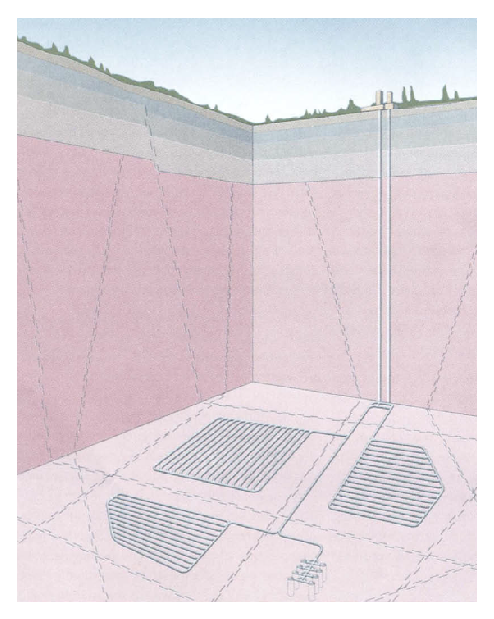
\includegraphics[width=0.6\textwidth, angle = 0]{nagra}
%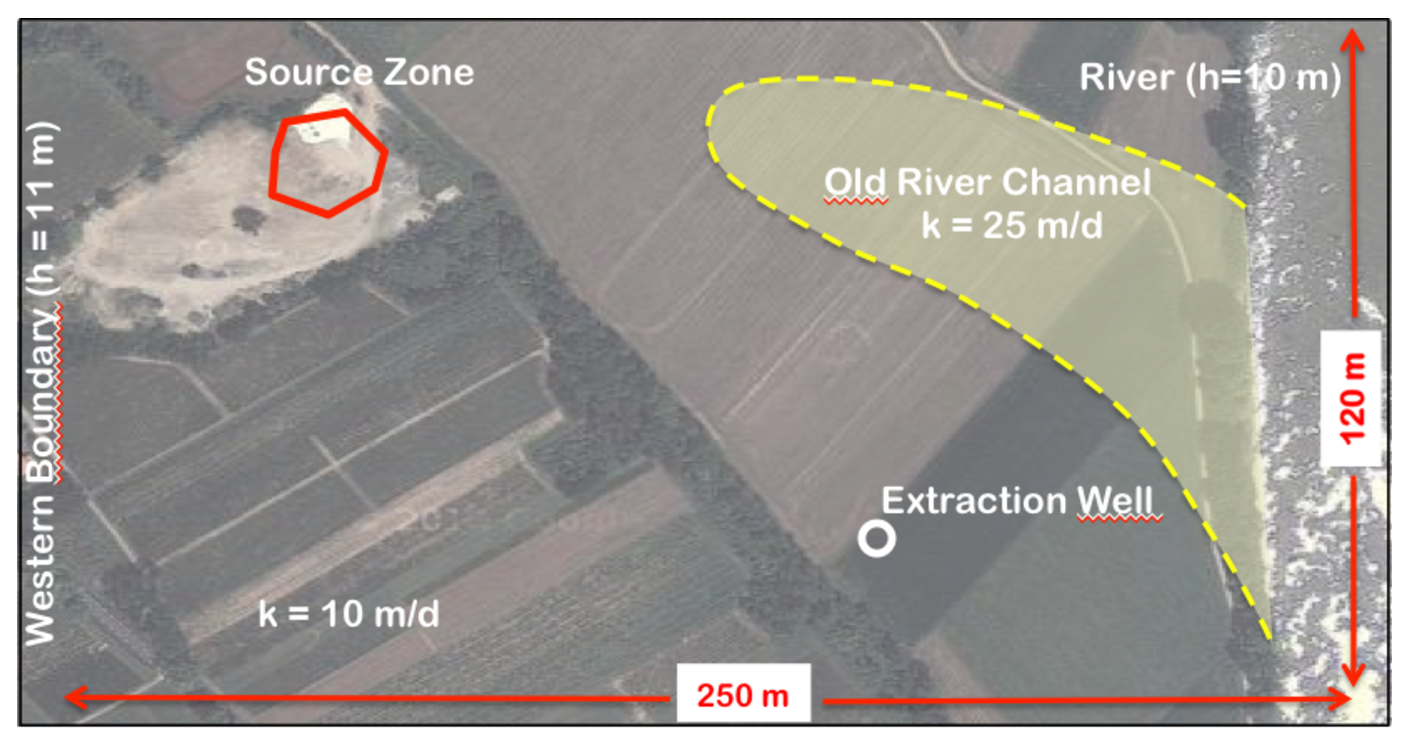
\includegraphics[height=0.3]{mt3dms_ex1_map.eps}
%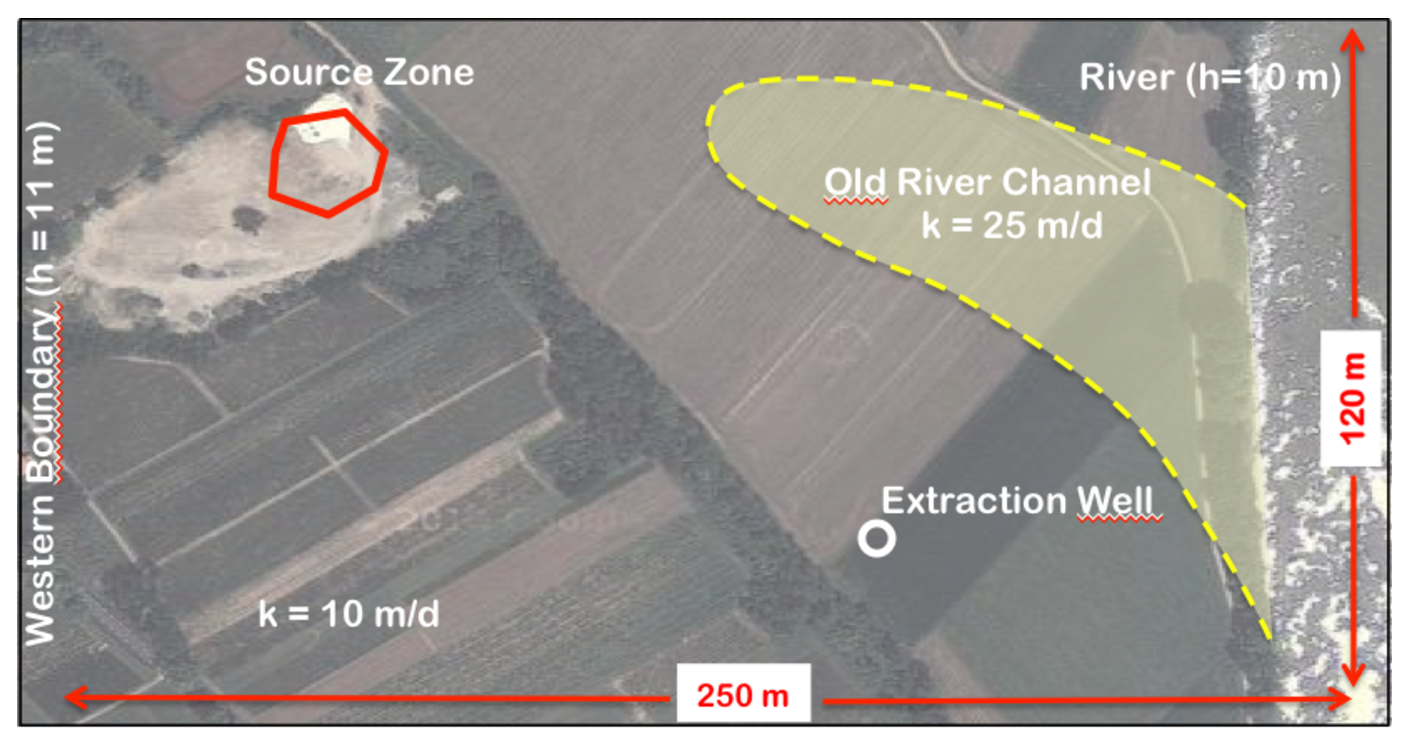
\includegraphics{mt3dms_ex1_map.eps}
\caption[Schematic illustration of geological disposal concept (source: NAGRA)]{Schematic illustration of geological disposal concept (source: NAGRA)}
\label{fig:nagra}
\end{figure}

However, due to the low hydraulic conductivity of clays,
following saturation, the main transport process is in this media is by molecular diffusion. 
In order to predict solute migration under conditions expected in a
repository, the diffusive behaviour within compacted bentonites
has been investigated in laboratory experiments for different species
(e.g., water, anions, cations, colloids) 
\citep{appelo_vanloon_2010, gimmi_2011, vanloon_2007, melkior_2009, sanchez_2008} 
among others; 
under different temperatures 
\citep{kozaki_1998, suzuki_2004, sanchez_2008}
and as a function of compaction \citep{suzuki_2004}. 
%(Pusch, 2002;  

\begin{figure}[ht]
\centering
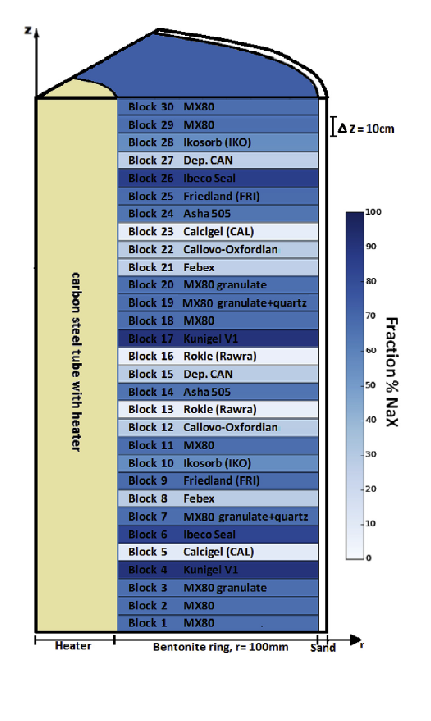
\includegraphics[width=0.6\textwidth, angle = 0]{bentonite_expt}
%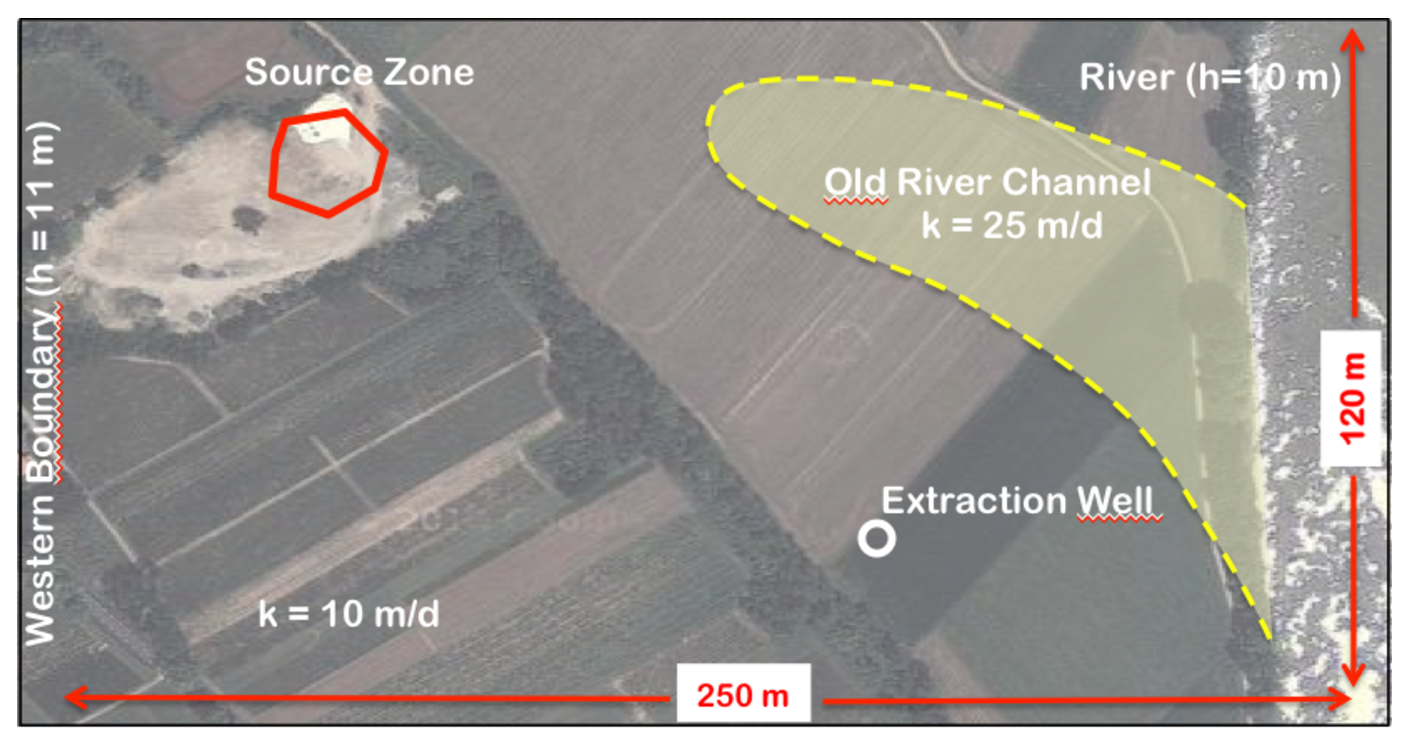
\includegraphics[height=0.3]{mt3dms_ex1_map.eps}
%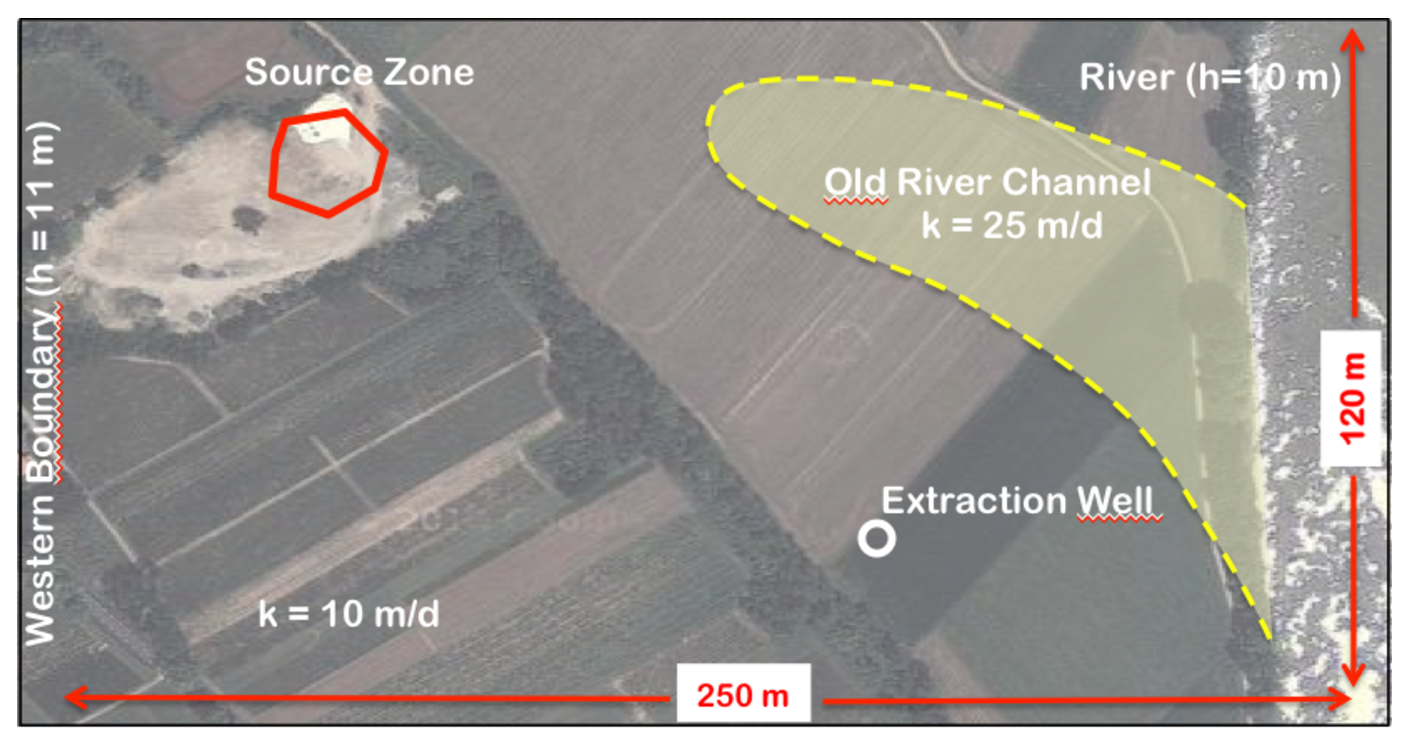
\includegraphics{mt3dms_ex1_map.eps}
\caption[ABM Experiment]{ABM Experiment}
\label{fig:abm}
\end{figure}

Nevertheless, the underlying phenomena controlling
diffusion within bentonites is still an active field of research,
including their mechanistic representation in numerical models.
%(Idiart and Pekala, 2016).
Uncertainties result from a lack of a well-established and widely
accepted conceptual model of the structure of compacted bentonite
at the nano-scale at different dry densities and salinities. Available
characterisation techniques for porosity distribution and nanostructure
of compacted bentonite often perturb the structure of
the water saturated bentonite and are therefore of limited applicability.
In addition, the validity of the classical Fickian diffusion
approach based on a single bulk (total) porosity has been questioned
in some cases, as it is unable to represent the diffusion of
cations, anions and neutral species simultaneously. As a result,
more complex mechanistic models have been proposed in the
literature to explain experimental data, based on different conceptualizations
of the pore space, e.g., \citep{birgersson_2009, appelo_vanloon_2010, gimmi_2011, tachi_2014}.

Solute mobility in compacted 
bentonites is further influenced by
geochemical reactions such as cation and anion exchange 
\citep{valter_2013, birgersson_2009, tachi_2014}, 
as well as the dissolution of primary minerals or the
precipitation of secondary phases \citep{arcos_2008, kaufhold_2013}, 
%(Liu and Neretnieks, 2006; 
%Idiart et al., 2013) 
which impact on the performance of bentonites as barriers 
by altering, e.g., the swelling capacity or the hydraulic and gas 
conductivities of these clays. 
In order to upscale laboratory findings and to test the
behaviour of bentonite clays under the thermo-hydraulic conditions
expected in radioactive waste repositories, several countries
are conducting large scale in-situ tests of engineered barrier systems.

In 2006 a field scale experiment was launched, the Alternative Buffer
Material (ABM) test 
%(Eng et al., 2007; 
\citep{svensson_2011}
, which extended investigations to a range of clays, including compacted
sedimentary clay materials (Friedland clay, Germany and Callovo-
Oxfordian clay, France) and various compacted bentonites. 

Three columns consisting of these different compacted clay buffer blocks
were installed in three boreholes (ABM1-3). The analysis of the first
package, ABM1 as illustrated in Figure \ref{fig:abm}, 
is the subject of this modelling exercise. 
The aim of the ABM1 test was to compare different clay materials 
and their performance over time when in contact with 
the heater, the seals, the fractured
host rock, and ambient groundwater at relevant depths as well as
the expected maximum in-situ temperatures. 
The main objective was to provide a basis for selecting an ideal 
buffer for the Swedish spent nuclear fuel repository. 
The experiment consists of a vertical borehole placed at
450 m depth \citep{svensson_2011}. 

It contains a central heater inside an iron tube surrounded by 11
different compacted clay blocks. The column of blocks was artificially
saturated with Aspo groundwater and heated to a maximum
temperature of 130 C. Over a duration of 28 months data were
recorded on the temperature and water pressure evolution.
Following the test, a comprehensive characterization of the cation
exchange population and distribution with time \citep{dohrmann_2013}
as well as mineralogical alterations \citep{kaufhold_2013} 
was carried out. All buffers started with distinctly different
exchangeable cation (EC) populations and it was expected that,
after the field experiment, the ECs would display horizontal variations
for all bentonite rings due to the radial heat distribution
induced by the central heater element. However, in contrast to this,
large scale variations in the ion exchange composition had
occurred. That is, the composition of exchangeable cations had
changed markedly in all clay materials over the whole test parcel
after 28 months, but no significant horizontal variations in the EC
populations within each ring was detectable. The most significant
change was an increase in exchangeable $Ca^{2+}$, and a decrease in
exchangeable $Na^{+}$ and Mg$^{2+}$. 
Mineralogical changes of the bentonites
were unable to explain these significant changes, and it was
postulated that interaction with the surrounding groundwater
must have caused partial equilibration of the porewater chemistry
within and possibly between the different bentonite blocks within
a short time frame \citep{dohrmann_2013}. 
%(Idiart et al., 2014; 
%Pekala et al., 2012)

In order to assess this hypothesis and to enhance the understanding
of the processes controlling the changes in porewater chemistry 
in bentonites under the influence of in-situ groundwater 
and heat conditions, a numerical model of the ABM1 
field test was developed.
For the modelling study the aim was (i) to develop a numerical model that
could provide a process-based description of the physical and
geochemical mechanisms controlling the chemical evolution of
bentonite porewaters at the field (i.e., meter) scale; 
(ii) to quantify the influence of groundwater on the chemical evolution of the
different clays with time, and (iii) to verify the model by applying it
to the available field data set collected during the ABM1 test.

The set-up of the ABM1 experiment, which is described in detail
in x 
%Eng et al. (2007) 
and \cite{svensson_2011}, 
consists of a central
steel canister with heaters, surrounded by ring shaped bentonite
blocks situated in a borehole of 300 mm diameter in crystalline
bedrock at about 450 m depth (Figure \ref{fig:abm}). 

Eleven different clay materials
(two sedimentary clays and nine bentonites) were included in
the ABM tests as compacted rings 
%(Table 1 and 
(Figure \ref{fig:abm}) 
with an outer diameter of 280 mm, and an inner diameter of 100 mm. 
Additionally, four rings were included which consisted of cloth-covered
steel-cages filled with bentonite pellets with and without additional
quartz to also test granulated material. All clay materials
were installed multiple times and the total number of material
blocks stacked on top of each other was 30 (Figure \ref{fig:abm}). 
Each block had a height of 100 mm, resulting in a total length of 3 m for the whole
ABM1 package. The gap between the ABM1 package and the crystalline
host rock was filled with sand, in which an artificial wetting
system was installed. This consisted of titanium tubes, connected to
a water tank, which supplied native 
Aspo groundwater over the
duration of the experiment. The wetting system was aimed at
simulating water bearing fractures within the host rock and supplied
ambient groundwater in addition to natural water inflow
through fractures into the deposit bore. However, the effectiveness
of the artificial wetting system to evenly supply groundwater to the
ABM1 package was open to question, as monitoring of applied
water pressure and injected water volume during the experiment
suggested leakage of injected water into the surrounding host rock
at some unknown depth within the bore \citep{svensson_2011}. 

The inflow of water through the fractures into the empty borehole was
measured at 3.6 l/hour before the test, but inflow locations were
not identified 
%(Eng et al., 2007). 
The ABM1 package was heated from the start of the experiment 
for the entire duration of the test
with exposure of the blocks to maximum temperatures of 130 C
for about one year (Figure \ref{fig:abm}). 

A heating element ran through the entire
axis of the ABM1 package with additional heaters being installed at
the top and bottom of the package to provide a relatively homogeneous
temperature distribution throughout the package length.
A chemical and mineralogical characterization of the different
clay materials was undertaken before the start of the test in order to
obtain a reference and to provide initial conditions before heating
and saturation \citep{svensson_2011}.
%Kumpulainen and Kiviranta, 2011)

After 28 months, the ABM1 experiment was terminated
and each block was sampled at five different radial distances from
the contact with the metal tube to record geochemical and
mineralogical alterations. Additionally, samples were collected at
three different vertical intervals in each block. It was found that,
apart from the EC distribution, almost all geochemical and mineralogical
alterations of the different clay materials were restricted to
a less than 5 mm wide zone from the interface between the central
steel canister and the blocks. Here, alterations included the accumulation
of Fe and organic carbon, the precipitation of carbonates
and gypsum/anhydride and the dissolution of some silicates
\citep{kaufhold_2013, wersin_2015}. 

Also, the cation exchange
capacity of the materials (CEC) showed little change compared to
the start of the test for most material blocks, with only 5 out of 30
showing a change of >5\% in CEC. 
In contrast, large scale alterations in the EC population 
had occurred in all blocks and modifications
occurred, without significant gradients over the entire horizontal
radial distance \citep{dohrmann_2013}.

\subsection[Basic numerical model setup]{Basic numerical model setup}

Based on the observed thermal and geochemical
changes during the ABM1 tests 
\citep{dohrmann_2013, kaufhold_2013, svensson_2011} 
%Idiart et al., 2014)
, 
we initially simulate a simplified subset of the processes that 
played during the experiment. We focus on the interaction between diffusive transport 
of the groundwater constituents and the cation exchange reactions that took place 
during the experiment. We exploit the radial symmetry of the experimental setup, 
which allows for considerable computational time savings compared to a fully 
three-dimensional setup.
Furthermore we simplify the problem by simulating only 3 different bentonite buffers
rather than the 11 different buffers that were included in the experiment and simulated
in \cite{wallis_2016}. A summary of the model setup is provided in Table \ref{wallis_setup}.
Note, that the circulating flow that occurred outside the bentonite rings was neglected.
Instead, the (constant) water composition of the circulating fluid was used to define 
a specified (constant) concentration boundary condition.  

\begin{itemize}

\item In ORTI, create a new model and save it in a new, separate directory.

\item Under {\color{blue}Parameters} $\rightarrow$ {\color{blue}Model} select the {\color{blue}Model} button and specify the attributes of the new model. Select the values {\color{blue}Radial} for {\color{blue}Dimension}, {\color{blue}unconfined} for {\color{blue}Type} 
and {\color{blue}MODFLOW series} for {\color{blue}Group} 

\item Under {\color{blue}Parameters} $\rightarrow$ {\color{blue}Model} select the {\color{blue}Grid} button and specify the details of the model domain and the spatial discretisation in the dialog that opens up. 
Define a (radial) transect that extends from Xmin = 0.05 to Xmax = 0.145m. 
For the vertical extent we consider Zmin = 0 to Zmax = 0.3m.  
The model domain may be discretised into grid cells of 5mm length and 1cm height. 
Note, that the model discretisation can be easily changed again later. 

\item Select {\color{blue}Parameters} and select the {\color{blue}Time} button.
Set the {\color{blue}Total Simulation Time} to 880 days and select a time {\color{blue}Step size}
of 5 days. 

\item Go to {\color{blue}Spatial Attributes} $\rightarrow$ {\color{blue}MODFLOW} $\rightarrow$ {\color{blue}LPF} $\rightarrow$ {\color{blue}lpf.8} to specify the horizontal hydraulic conductivity to 0.001 $m/day$.
Note that the entered hydraulic conductivity will not affect the results as the groundwater will not move
in this example. 

\item Go to {\color{blue}Spatial Attributes} $\rightarrow$ {\color{blue}MODFLOW} $\rightarrow$ {\color{blue}LPF} $\rightarrow$ {\color{blue}lpf.9} to specify the vertical hydraulic conductivity to 0.001 $m/day$

\item Go to {\color{blue}Spatial Attributes} $\rightarrow$ {\color{blue}MT3DMS} $\rightarrow$ {\color{blue}BTN} $\rightarrow$ {\color{blue}btn.11} and specify a uniform effective porosity of 0.45, even though the 
porosities of the various bentonites used in the ABM test varied slightly \citep{wallis_2016}.   


\item Given that there is no groundwater flow involved in this example there is in principle no need to define any hydraulic boundary conditions. However, for numerical reasons we define a specified head boundary at a single point by going to {\color{blue}Spatial Attributes} $\rightarrow$ {\color{blue}MODFLOW} $\rightarrow$ {\color{blue}BAS6} $\rightarrow$ {\color{blue}bas.3 Boundary Conditions} and setting the value to -1 (= active cell) at X = 0.00525 m and 0.006 m in vertical direction. 

\item We will also define a global initial hydraulic head for the entire domain (Background value) by going to {\color{blue}Spatial Attributes} $\rightarrow$ {\color{blue}MODFLOW} $\rightarrow$ {\color{blue}BAS6} $\rightarrow$ {\color{blue}bas.6 Initial Heads} and set the
 {\color{blue}Backg.} value to 1m. Then press {\color{blue}'OK'} to confirm the value.

\end{itemize}

Again, as there will not be any groundwater flow this input is solely made for numerical reasons.
For the same reason MODFLOW needs to be executed before the next stage of the model setup.

\begin{itemize}

\item Under {\color{blue}Parameters} $\rightarrow$ {\color{blue}Flow} use the {\color{blue}Write Button} to write all the input files required to run MODFLOW

\item Under {\color{blue}Parameters} $\rightarrow$ {\color{blue}Flow} use the 
{\color{blue}Red Arrow} button to start the MODFLOW simulation   

\end{itemize}

\begin{table}[t]
\caption{Model geometry and summary of key input parameters.}
\begin{center}
\begin{tabular}{lc} 
\toprule
Simulation type                     & steady state \\
Total simulation period\ $ (days)      $         &  880            \\
Time step length\ $ (days)      $         &  10            \\
Model \  length\ $ (m)      $         &  0.095            \\
Model \  thickness\ $(m)$                        &  0.3            \\
Grid \ spacing\ $\Delta x $ $(m)$                &    0.005            \\
Grid \ spacing\ $\Delta z $ $(m)$                &    0.01            \\
Porosity\     $            $         &  0.5           \\
Horizontal hydraulic conductivity\ $(m/day)$               &  0.001        \\ 
Vertical   hydraulic conductivity\ $(m/day)$               &  0.001         \\ 
Longitudinal dispersivity\ $(m)                 $         &  0.01          \\ 
Transverse  vertical dispersivity\ $(m)         $         &  0.01          \\ 
Diffusion coefficient\ $(m)         $         &  $5 \times 10^{-10}$          \\ 
\bottomrule
\end{tabular}
\label{wallis_setup}
\end{center}
\end{table}
    
\subsection[Diffusion model setup]{Diffusion model setup}

In the absence of groundwater flow inside the model domain molecular 
diffusion acted as the only transport process while neither advection 
nor hydrodynamic dispersion occurred. \cite{wallis_2016} found that the
temporal and spatial variations of the temperature-field 
had a significant impact on the diffusion rates.
To consider this effect they incorporated the temperature-dependency
of the diffusion coefficient into their model framework and obtained, 
as a result, a significantly improved match with
observed concentration data. For simplicity we neglect this dependency in this 
modelling exercise while generally it would need to be considered.     
 
\begin{itemize}

\item Go to {\color{blue}Parameters} $\rightarrow$ {\color{blue}Transport} 
and select the {\color{blue}Parameter} button


\item Select {\color{blue}Spatial Attributes} $\rightarrow$ 
{\color{blue}MT3DMS} $\rightarrow$ {\color{blue}DSP}, 
enter a diffusion coefficient of 4.32 $\times$ $10^{-5}$ $m^2$ $days^{-1}$ 
and then don't forget to click {\color{blue}OK} 

\end{itemize}
	

\begin{figure}[t]
\centering
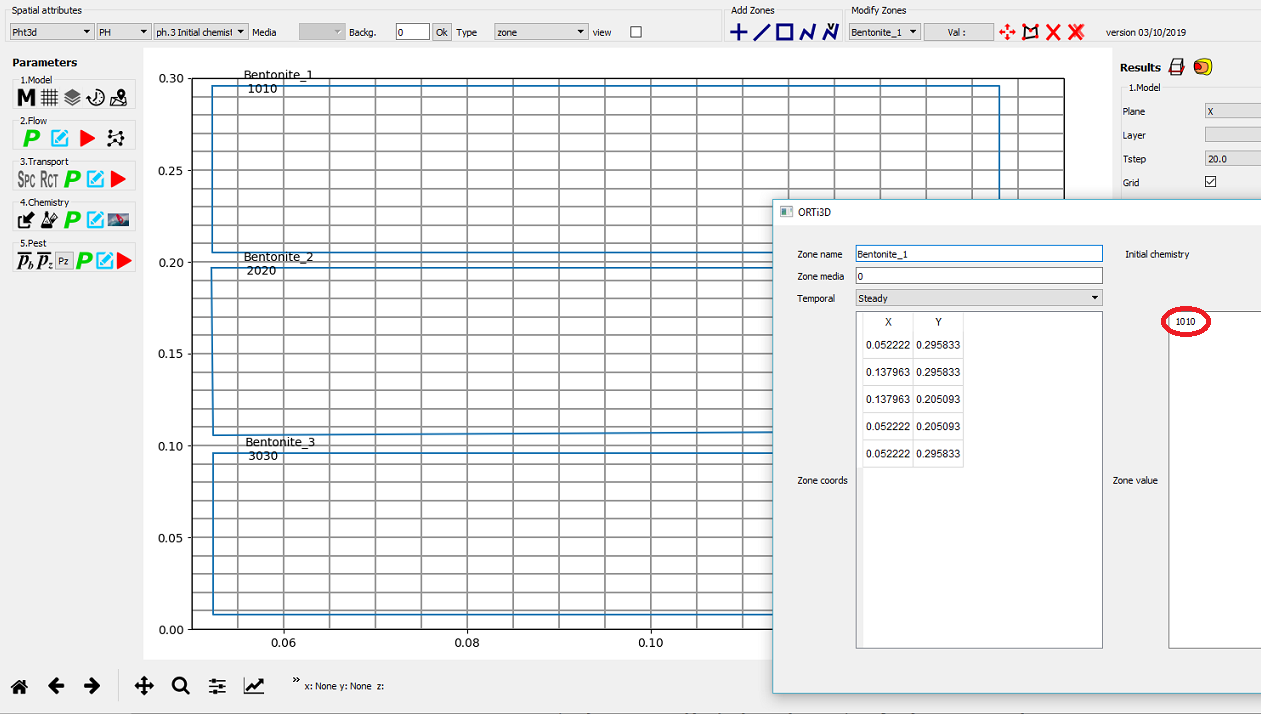
\includegraphics[width=1.0\textwidth, angle = 0]{bento_zones}
%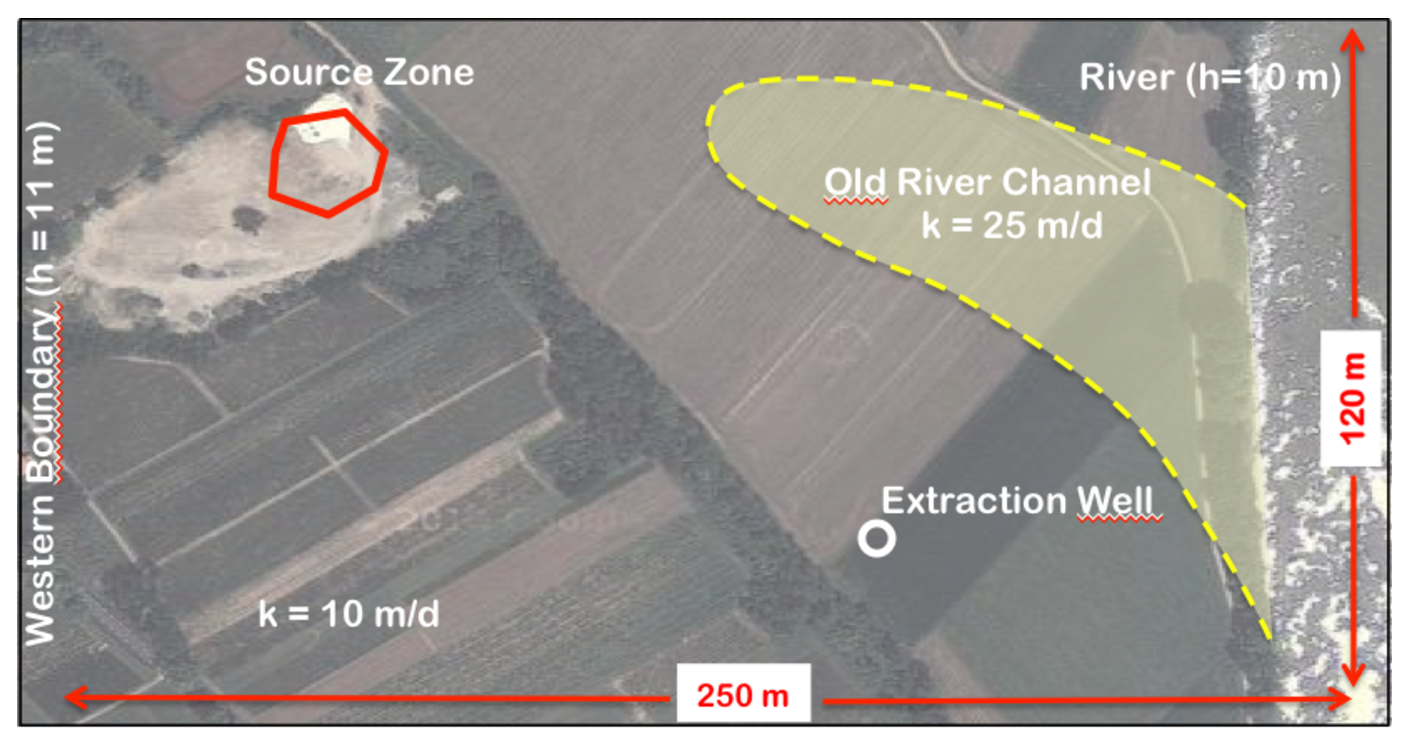
\includegraphics[height=0.3]{mt3dms_ex1_map.eps}
%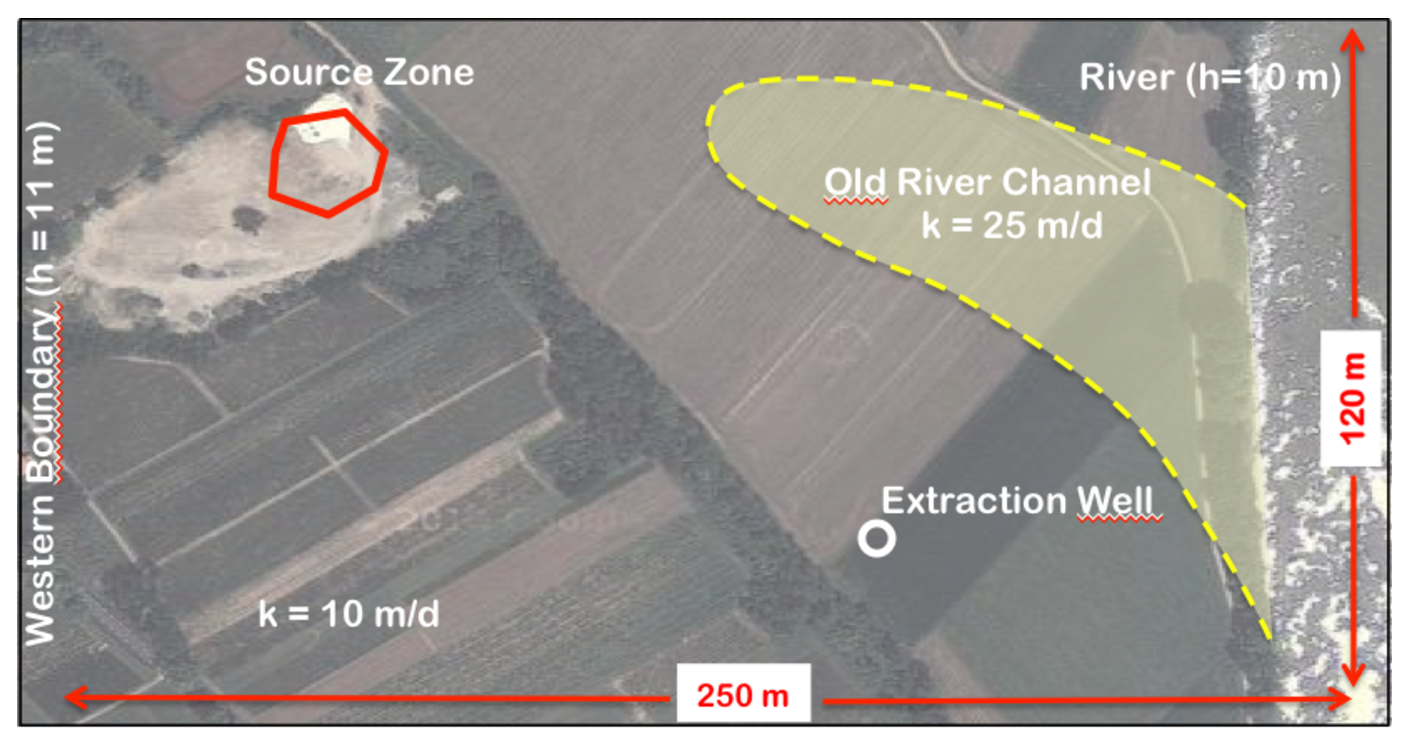
\includegraphics{mt3dms_ex1_map.eps}
\caption[Position of Initial Chemistry zones]{Position of Initial Chemistry zones}
\label{fig:bento_zones}
\end{figure}

\begin{table}[b]
\caption{Solution compositions to define the initial water compositions and of the fluid circulating outside the bentonite rings.}
\begin{center}
\begin{tabular}{l c c c c}
\hline
 Aqueous      & $C_{Backgr}$            & $C_{init}$               & $C_{init}$                & $C_{init}$  \\
 Component    & $(mol\ l^{-1}_w)$       & $(mol\ l^{-1}_w)$        & $(mol\ l^{-1}_w)$         & $(mol\ l^{-1}_w)$   \\ \hline
 C(4)         & 8.600 $\times$ $10^{-4}$  & 8.890 $\times$ $10^{-4}$ & 8.890 $\times$ $10^{-4}$  & 8.890 $\times$ $10^{-4}$\\
 Ca           & 6.479 $\times$ $10^{-2}$  & 1.017 $\times$ $10^{-2}$ & 2.373 $\times$ $10^{-2}$  & 4.525 $\times$ $10^{-3}$\\
 Cl           & 2.332 $\times$ $10^{-1}$  & 2.332 $\times$ $10^{-1}$ & 2.332 $\times$ $10^{-1}$  & 2.332 $\times$ $10^{-1}$ \\
 K            & 3.220 $\times$ $10^{-4}$  & 2.146 $\times$ $10^{-3}$ & 2.213 $\times$ $10^{-3}$  & 1.339 $\times$ $10^{-3}$\\
 Mg           & 2.704 $\times$ $10^{-3}$  & 1.653 $\times$ $10^{-3}$ & 2.232 $\times$ $10^{-3}$  & 2.423 $\times$ $10^{-3}$\\
 Na           & 1.090 $\times$ $10^{-1}$  & 2.185 $\times$ $10^{-3}$ & 1.500 $\times$ $10^{-1}$  & 2.291 $\times$ $10^{-3}$ \\ 
 S(6)         & 5.100 $\times$ $10^{-3}$  & 5.100 $\times$ $10^{-3}$ & 5.100 $\times$ $10^{-3}$  & 5.100 $\times$ $10^{-3}$\\ 
 pH           &   7.330	                  &  7.479                   & 7.390                     & 7.499 \\
 pe           &   4                       &  4                       &   4                       & 4     \\ \hline
\end{tabular}
\label{ex_wallis_aqu_conc}
\end{center}
\end{table}
	

\begin{table}
\caption{Initial exchanger compositions associated with the 3 different bentonite rings.}
\begin{center}
\begin{tabular}{l c c c}
\hline
 Exchanger   & $C_{init}$ Assembl 1     & $C_{init}$  Assembl 2     & $C_{init}$  Assembl 3 \\
 Species     & $(mol\ l^{-1}_w)$        & $(mol\ l^{-1}_w)$         & $(mol\ l^{-1}_w)$   \\ \hline
 CaX2        & 2.290 $\times$ $10^{-1}$ & 6.281 $\times$ $10^{-1}$  & 3.244 $\times$ $10^{-1}$\\
 KX          & 3.768 $\times$ $10^{-2}$ & 5.444 $\times$ $10^{-2}$  & 5.458 $\times$ $10^{-2}$\\
 MgX2        & 7.636 $\times$ $10^{-2}$ & 3.690 $\times$ $10^{-1}$  & 1.081 $\times$ $10^{-1}$\\
 NaX         & 1.315  & 7.370 $\times$ $10^{-1}$  & 1.865 \\
\end{tabular}
\label{ex_wallis_ex_conc}
\end{center}
\end{table}


\subsection[Reactive transport]{Reactive transport}
	
\begin{itemize}

\item Copy the database file {\color{red} \textbf{pht3d\_datab.dat}} 
that is provided for this exercise 
into the folder that will contain all files for this exercise.

\item Go to {\color{blue}Parameters} $\rightarrow$ {\color{blue}Chemistry} and select the
{\color{blue}Import database} button. ORTI will then read and interpret 
the PHT3D database file.

\item In this next step the initial concentrations of the aqueous components need to be defined. 
The initial concentrations vary between the 3 different bentonite rings and therefore three different
water compositions need to be entered as {\color{red} \textbf{Solutions 1-3}}. 
Furthermore the composition of the water that is circulating 
outside the bentonite rings is entered as the {\color{red} \textbf{Backgr}} solution. 
The water compositions are listed in Table \ref{ex_wallis_aqu_conc}.
Note, that the {\color{blue}Solution} and other Tabs allow you to copy/paste 
concentrations values from external, e.g., Excel tables. 
All 4 solutions are entered under the {\color{blue} \textbf{Solutions}} Tab.
In that Tab first activate all relevant species by ticking the appropriate boxes for 
$pH$, $pe$,  $C(4)$, $Ca$, $Cl$, $K$, $Mg$, $Na$ and $S(6)$

\item In addition the initial concentrations of the four exchanger-species, i.e., $CaX2$, 
$KX$, $MgX2$ and $NaX$ need to be entered for {\color{red} \textbf{Assembl1}}, 
{\color{red} \textbf{Assembl2}} and {\color{red} \textbf{Assembl3}}, respectively,
after activating the species. 
The initial exchanger compositions are listed in Table \ref{ex_wallis_ex_conc}.
Note, that the initial exchanger composition and the initial aqueous composition 
provided in Table \ref{ex_wallis_ex_conc} are already in geochemical equilibrium.   
That implies that in the absence of transport processes no reaction would proceed.      

\item In the next step we need to define where the aqueous solutions 
and the exchanger compositions will be employed. 

\item First, {\color{red} \textbf{Backgr}} will be used to define a specified 
concentration boundary condition at the outer fringe of the bentonite ring.
This reflects the fact that the circulating water outside the bentonite rings 
maintains a constant water composition. This is implemented by 
defining the boundary type under {\color{blue}Spatial Attributes} $\rightarrow$ {\color{blue}MT3DMS} $\rightarrow$ {\color{blue}BTN} $\rightarrow$ {\color{blue}btn.12} and specify a boundary 
type as -1 (= specified concentration boundary) along a vertical line near the outer fringe (x = 0.1425).
Define a name for the boundary (such as bc\_circulation\_wq) in the dialogue.
Secondly, we need to make sure that the {\color{red} \textbf{Backgr}} water composition
is used at this boundary. To do this we normally need to define the initial water chemistry 
at the same location (here a line) as the boundary condition type. 
However, given that the {\color{red} \textbf{Backgr}} water composition is used 
as the default water composition at all location where no other initial chemistry is defined,
there is in this case no need to explicitly define the water composition for this boundary.   

\item Finally, the different initial water and cation exchanger compositions are implemented
through defining three different {\color{blue}Initial Chemistry} zones, with each 
of the three zones corresponding to one of the 0.1m thick bentonite rings.  
Define the 3 zones by going to 
{\color{blue}Spatial Attributes} $\rightarrow$ 
{\color{blue}PHT3D} $\rightarrow$ 
{\color{blue}PH} $\rightarrow$ {\color{blue}ph.3} and define one after another 
of the 3 {\color{blue}Initial Chemistry} zones (see Figure \ref{fig:bento_zones}). 
For the uppermost zone (first bentonite ring) allocate a {\color{blue}Zone Value} of {\color{red} \textbf{1010}}, 
allocate {\color{red} \textbf{2020}} for the central zone (second bentonite ring) and allocate 
{\color{red} \textbf{3030}} for the zone in which the bottom bentonite ring is located.
Setting the {\color{blue}Zone Value} to 3030 means that in this zone the chemistry is defined
through the aqueous {\color{red} \textbf{Solution 3}}, {\color{red} \textbf{Mineral assemblage 0}},
exchanger composition {\color{red} \textbf{Assembl 3}} and Surface {\color{red} \textbf{Site 0}}.
No mineral or surface complexation reactions are considered in the reaction network,
which is implemented by not activating any mineral phases or surface sites in the respective Tabs.  
 
\item Now run PHT3D.

\item Inspect the results by plotting concentration profiles of $NaX$ and $CaX2$ for 
specific simulation times. 

\item What would happen if you plotted the sum of $NaX$, $CaX2$, $KX$ and $MgX2$ ?

\item Plot aqueous and exchanger species concentrations at selected distances from the heater element and interpret the breakthrough curves as wel as the differences between the 3 bentonites.   

\end{itemize}	








%\chapter{Surface complexation reactions}
\def\shorttitle{Surface complexation reactions} % Abbreviated chapter title for right top header

\section{Background}


Oxides, hydroxides and organic matter carry functional groups at their surface, 
which  enable them to sorb cations, anions, and neutral species from solution.  
Typically, these functional groups behave as Bronsted acids and/or bases, 
which is to say they can accept hydrogen ions, release hydrogen ions, or, 
in some cases, both. The sorption behaviour depends on the type 
of mineral, crystal morphology, even which crystal face(s) dominate, 
as well as the composition and pH of the solution.
In response to uptake/release of hydrogen or other ions from/to solution, 
a net charge on the surface develops.

It can be shown that for a dissociation reaction (Appelo and Postma, 2005):
\begin{equation}
\log K_{\text{a}} = \log K_{\text{int}} + \frac{zF\psi_0}{RT \ln 10}
\end{equation}
in which $K_{\text{a}}$ is the apparent dissociation constant, $K_{\text{int}}$ is the intrinsic dissociation constant, $z$ is the charge of the ion, $F$ the Faraday constant (96,485 C/mol), $\psi_0$ the potential at the surface, $R$ the gas constant (8.314 J/K/mol) and $T$ the absolute temperature.

The intrinsic dissociation constant, $K_{\text{int}}$, applies to the chemical binding of the ion and the surface. The PRHEEQC database contains a compilation by Dzombak and Morel (1990) of laboratory-determined values of intrinsic dissociation constants for hydrous ferric oxide.

The apparent dissociation `constant' ($K_{\text{a}}$), however, varies with the potential and thus the charge at the surface. In order to calculate the $K_{\text{a}}$, the $\psi_0$ needs to be known. PHREEQC uses a double-layer model to relate the charge density on the surface ($\sigma_s$) with ionic strength ($I$, equation \ref{eq:ionic_strength}) and $\psi_0$ \citep{phreeqc2}.

\section{PHREEQC Exercise 5: Surface complexation reactions}
\subsection{Calculation of a charged surface composition}
This exercise demonstrates the use of the \textbf{SURFACE} keyword, which is used in PHREEQC for surface complexation calculations. The input file has already been prepared and is called {\color{red}kd\_surf.phrq}. The definition of the surface is as follows:

\begin{quote}
	SURFACE 1 \\
	Hfo\_w	2e-4	600	0.088 \\
	Hfo\_s	5e-6 \\
	-equilibrate 1 
\end{quote}

The names {\color{red}Hfo\_w} and {\color{red}Hfo\_s} correspond to the names of the master species in the PRHEEQC database that refer to the weak- and the strong surface sites, respectively. The number that follows is the number of surface sites in moles. For the weak sites, the surface area (600 m$^2$/g) and mass of ferrihydrite (88 mg) are also specified. Unless these values are explicitly typed for Hfo\_s as well, they apply to both the weak and the strong sites.

The input file contains BASIC statements that control the output to a text file in spreadsheet format. The distribution coefficient of Zn is calculated for both the weak and the strong sites, as well as an overall distribution coefficient. The file is called {\color{red}kd\_surf.prn} and can be opened in the Grid tab of PRHEEQC for Windows after the calculation has finished.

What is the value of the overall distribution coefficient for Zn? 

Answer: $K_d$ = \ldots\ldots.

Test the effect on the $K_d$ of:

\begin{itemize}

\item doubling the Zn concentration? Answer: $K_d$ = \ldots\ldots.

\item doubling the Mg concentration? Answer: $K_d$ = \ldots\ldots.

\item doubling the amount of ferrihydrite? Answer: $K_d$ = \ldots\ldots.

\item changing pH from 7 to 5? Answer: $K_d$ = \ldots\ldots.

\end{itemize}

\subsection{Uranium sorption at the Hanford site}

This exercise is based on uranium sorption over the range of chemical 
conditions at the Hanford 300 area in Richland, Washington, United States.  
You will simulate uranium sorption on hydrous ferric oxide under three 
sets of chemical conditions: groundwater with a large Columbia River signal, 
Hanford groundwater with moderate $Ca$ concentrations, 
and Hanford groundwater with high $Ca$.

Use the provided input file template to construct the 
input file ({\color{red}\textbf{SCM\_Exercise\_Template.xlsx}}).  
The template has the thermodynamic data for $Ca$- and $Mg-U(6)-CO3-2$ solution species.  
It also has thermodynamic data for the $U(6)$ sorption on hydrous ferric 
oxide from \cite{mahoney_2009}, 
who fit the best available data for $U(6)$ sorption 
on hydrous ferric oxide in the presence and absence of 
$CO_2$ using the thermodynamic data from the Wateq4f database.  

The simulation is based on the following set of laboratory batch experiments
\begin{itemize}
\item Equilibrate hydrous ferric oxide with {\color{red}\textbf{Groundwater 2}} that does not have uranium;
\item React the equilibrated hydrous ferric oxide with {\color{red}\textbf{River}} 
composition, which represents groundwater with a large Columbia River signal;
\item React the equilibrated hydrous ferric oxide with {\color{red}\textbf{Groundwater 1}} 
composition, which represents groundwater from the Hanford formation with moderate Ca concentration;
\item React the equilibrated hydrous ferric oxide with {\color{red}\textbf{Groundwater 2}} 
composition, which represents groundwater from the Hanford formation with high $Ca$.
\item Enter the solution composition for {\color{red}\textbf{Groundwater 2}} 
but without $U(6)$ under {\color{red}\textbf{SOLUTION 1}}.  
This will be used to equilibrate the hydrous ferric oxide before reacting 
with $U(6)$-containing groundwater compositions.  
Enter the compositions of the three groundwater datasets from 
Table \ref{tab:hanford1}
under {\color{red}\textbf{SOLUTION 10}}, 
{\color{red}\textbf{SOLUTION 50}}, 
and {\color{red}\textbf{SOLUTION 55}}, respectively.  
\end{itemize} 

\begin{table}[h]
\begin{center}
\centering
\caption{Groundwater compositions for the Hanford surface complexation exercise}
\begin{tabular}{cllll}
\toprule
Parameter  	& River	& Groundwater 1	& Groundwater 2	& Units/comment \\
pH	        & 6.00	& 8.11	        & 8.11	        & NIST/Fix \\
Temperature	& 21	  & 21	          & 21	          & $^\circ$C  \\
Alkalinity	& 0.164	& 5.00	        & 5.00	        & mmol/L \\
Na	        & 3.9	  & 6.8	          & 6.8	          & mmol/L \\
K	          & 0.15	& 0.2	          & 0.2	          & mmol/L \\
Mg	        & 0.5	  & 0.4	          & 0.4	          & mmol/L \\
Ca	        & 0.5	  & 0.5	          & 5.5	          & mmol/L \\
Cl	        & 1.49	& 1	            & 11	          & mmol/L charge \\
S(6)	      & 2.2	  & 1.4	          & 1.4	          & mmol/L \\
N(5)	      & 0	    & 0	            & 0	            & mmol/L \\
U(6)	      & 0.001	& 0.001	        & 0.001	        & mmol/L \\
\bottomrule
\end{tabular}
\label{tab:hanford1}
\end{center}
\end{table}

The keyword used for entering data for the surface assemblage is {\color{red}\textbf{SURFACE n}}.  
The required information is the name of the site, the moles of that site, 
the specific surface area (m2/g) of the solid, and the number of 
grams of the solid in the simulation.  
The specific surface area (SSA) and grams of solid (grams) 
are needed for calculating the coulombic term in the diffuse layer model.  
Under the {\color{red}\textbf{SURFACE 1}} keyword, 
enter the required data, which are in Table \ref{tab:hanford2}.

\begin{quote}
{\color{red}SURFACE 1} \\
\# Site	moles	SSA	grams \\
\end{quote}

\begin{table}[h]
\begin{center}
\centering
\caption{Concentrations of sorption sites and other data required for simulating surface complexation for this exercise}
\begin{tabular}{clll}
\toprule
Site name	& Moles of site              	& SSA (m2/g)	& Grams of HFO \\
Hfo\_s	  & 5.62 $times$ 10$^{-6}$	    & 600	        & 0.10 \\
Hfo\_w	  & 2.25 $times$ 10$^{-4}$	    & 600       	& 0.10 \\
\bottomrule
\end{tabular}
\label{tab:hanford2}
\end{center}
\end{table}

Below the section where the groundwater 
compositions and surface assemblage data are entered 
is a datablock to create a user-defined
{\color{red}\textbf{SELECTED\_OUTPUT}} file.  
This file simplifies determining the simulated sorbed $U(6)$ 
under the three sets of chemical conditions.

Below the {\color{red}\textbf{SELECTED\_OUTPUT}} file block, 
run the simulation. Using the {\color{red}\textbf{USE SURFACE 1}} 
and {\color{red}\textbf{USE SOLUTION n}} keywords 
(followed by an {\color{red}\textbf{END}} statement), 
react the equilibrated surface assemblage with the river-dominated groundwater, 
the Hanford aquifer groundwater with moderate $Ca$, 
and the Hanford groundwater with high $Ca$. 

The {\color{red}\textbf{SELECTED\_OUTPUT}} file will be written in the directory with the input file.  
Open the {\color{red}\textbf{SELECTED\_OUTPUT}} file 
with Excel and answer the following questions.

\begin{itemize}
\item What is the concentration of dissolved $U$, sorbed $U$, 
and percent of the total $U$ sorbed under each of set of conditions ?  
\item How did the pH change during reaction with of the surface assemblage with each of the groundwater compositions ?
\end{itemize}
%\section[PHT3D Exercise 6, Zinc transport at the Cape Cod site]{PHT3D Exercise 6, Zinc transport at the Cape Cod site}

In this exercise we will construct a model that provides 
a good example for the consideration of surface complexation reactions in PHT3D.
The example is based on a modelling study for the Cape Code site, 
The full details of this study were reported in \cite{Kent20003411}.    
The Cape Cod research site is near a wastewater-treatment facility at 
the Massachusetts Military Reservation (MMR). A treated-sewage plume originated 
from the facility's infiltration beds, which were used from about 1936 to 1995. 
At the time the modelling study was undertaken the plume at the site extended 
more than 6 kilometers from the disposal site in the 
sand and gravel aquifer. The plume contains a complex mixture of phosphate, nitrate, 
metal ions (such as zinc), detergents, organic chemicals, and microbes. 
Over many years the plume and adjacent parts of the aquifer  
served as a field laboratory for a multidisciplinary team of scientists 
who investigated many fundamantal aspects 
of contaminant transport behaviour.

\subsection{Background: Groundwater Flow}

At the Cape Cod site the regional groundwater flow is generally towards 
the south, but locally the flow direction is directed from the 
sewage treatment facility towards the eastern shore of Ashumet Pond.  
The groundwater flow is nearly horizontal.
Approximately 25 cm/yr of areal recharge results
in a small vertical component to flow as well as
in the accumulation of a lens of pristine groundwater on top of 
the sewage plume, the thickness of which increases with 
distance away from the sewage 
treatment plant \citep[]{Leblanc1984,Leblanc1991895}.  
The magnitude of the hydraulic gradient 
is approximately 1.7 m/km. 
Seasonal fluctuations in the flow system result in small 
variations (approximately 0.2 m/km) in the magnitude
of the gradient as well as in small annual fluctuation 
in flow direction.

\subsection{Background: Hydrogeochemistry}

Contrasting chemical conditions between sewage-contaminated
and ambient groundwater gave rise to longitudinal and 
vertical gradients in groundwater chemistry. 
The ambient groundwater surrounding the sewage plume had 
high concentrations of dissolved oxygen, pH values 
in the range 5.3-5.8, and low concentrations of dissolved salts 
\citep[]{Leblanc1991895,Hess1996,Kent1999293}.
%[LeBlanc  et  al., 1991; Hess  et al., 1996; Kent and Maeder, 1999].
Sewage-contaminated groundwater under the disposal beds had high 
concentrations of nitrate.
Concentrations of dissolved oxygen successively decreased with depth 
\citep[]{Smith1991285,Smith19911815}.
%[Smith et al., 1991a].  
Biodegradation of organic matter in conjunction with solute transport 
away from the disposal beds resulted in the depletion of dissolved oxygen 
throughout the plume and the depletion of nitrate, followed by 
the accumulation of dissolved Fe(II), in the core of the plume 
%[Smith et al., 1991b; Kent  et  al., 1994]
\citep[]{Smith1991285,Kent19941099}. 
 
These biodegradation reactions influenced the pH  
within the aquifer zone affected by the sewage plume 
%[Abrams et al., 1998; Abrams and Loague, 2000b].
\citep[]{Abrams19981531,Abrams20002015}.
The principal chemical process in terms of controlling Zn transport is 
assumed to be Zn adsorption onto the sediments.
A single reaction with the stoichiometry could already adequately 
describe the pH effect observed in laboratory batch studies of
Zn adsorption onto the sediments \citep[]{Davis19982820}:

\begin{equation}
Zn^{2+}  +  >SOH    =  >SOZn^+  + H^+,  log  ^SQ_{SOZn}  
\label{eq:zn_single_site}
\end{equation} 

Adding a second surface site with the same reaction stoichiometry results in an  
SCM that can fit both the pH and Zn-concentration 
effect \citep[]{Davis19982820}.
This so-called two-site approach was one of the various
numerical implementations tested by \cite{Kent20003411}.
This two-site model will be used in the present exercise.
In the two-site SCM a small percentage of the total 
adsorption sites are considered to have a much greater affinity 
for adsorption ("strong sites," $>SsOH$) than the rest of the 
sites ("weak  sites," $>SwOH$): 

\begin{equation}
Zn^{2+}  +  >S_sOH    =  >S_sOZn^+  + H^+,  log  ^SQ_{S_sOZn}  
\label{eq:zn_strong_sites}
\end{equation} 

\begin{equation}
Zn^{2+}  +  >S_wOH  =  >S_wOZn^+  + H^+,  log  ^SQ_{S_wOZn}   \\
\label{eq:zn_weak_sites}
\end{equation} 

Before proceeding, it is worthwhile to consider the standard state for sorbed species 
in surface complexation models. 
The same standard state used for aqueous species - either 1 mole of surface complex \textbackslash L of solution (M)or \textbackslash kilogram water (m) - is often used for surface complexes as well. For example, the comprehensive compilation of equilibrium constants for sorption on hydrous ferric oxide by \cite{Dzombak1990} adopts a standard state of 1 M for sorbed species.  
One should be aware, however, there is a pitfall associated with this choice of 
standard state %\citet{appelo_postma_1999})
\citep[e.g.,][]{appelo_postma_1999}. 
The pitfall can be illustrated by considering a batch reactor with a suspension in sorptive equilibrium. 
In this thought experiment, we allow all of the solids to settle to the bottom of 
the reactor once sorptive equilibrium has been achieved, then we remove half of the solution without removing any solid.
Sorbed concentrations expressed in moles/kg water have now increased by a factor of two because the volume of solution (hence, mass of water) 
has decreased by a factor of two with no change in the amount of the solid.  
For surface complexation reactions such as those described the Eqn. \ref{eq:zn_strong_sites} 
and Eqn. \ref{eq:zn_weak_sites}, 
the concentration of sorbed Zn doubles and the concentration of free surface functional groups double,
so the factor of two cancels out in the mass action expression.  
For this type of surface complex - 
called ''monodentate'' (one surface site per sorbed species) -
the choice of standard state for sorbed species does not affect the value of the equilibrium constant. 
However, for ''bidentate'' surface complexes, where there are two surface functional groups 
bound to a single sorbing species, the situation is more complicated.  
Consider formation of a bidentate surface complexation analogous 
to Eqn. \ref{eq:zn_strong_sites}:

\begin{equation}
Zn^{2+}  +  2>S_sOH    =  (>SsO)2Zn + 2H^+  \\
\label{eq:zn_2}
\end{equation}

The mass action expression can be written with the concentration 
of the Zn surface complex raised to
the first power in the numerator and concentration of free surface 
sites squared in the denominator.  
In this mass action expression, the factor of two does not cancel out.  
This observation can be generalized by stating that equilibrium constants describing sorption where multidentate surface complexes are involved are a function of the solid to liquid ratio if a standard
state of 1 M or 1 m is adopted for sorbed species.  
There has been much discussion of this in the literature %(e.g.,\citet{wang_giammar_2013})
\citep[e.g.,][]{wang_giammar_2013}.  
To avoid this pitfall, PHREEQC adopts a standard state for sorbed species whereby the fraction 
of sites occupied by a given sorbed species equals 1.
In reaction \ref{eq:zn_2}, the relationship between sorbed Zn 
in units of moles \textbackslash kg water and 
sorbed Zn in units of mole fraction occupied 
sites is 
\begin{equation}
XZn = 2[(>SsO)2Zn]/[SsOHT],  \\
\label{eq:xzn}
\end{equation}
where square brackets refer to concentrations in moles/kg water and SsOHT is the total 
concentration of strong sorption sites.  
The factor of two results from the fact that the surface complex covers two sites.  
Therefore, when using equilibrium constants for multidentate sorbed species taken 
from the literature in a transport simulation, it is important to insure 
that either the equilibrium constant uses mole fraction of sites occupied 
by any given sorbed species = 1 or is properly converted to that standard state.  
Formulas for making such conversions are presented 
in various papers 
%\citep[see][]{jon90} 	    -->    	(see Jones et al., 1990)
\citep[e.g.,][]{wang_giammar_2013}.

\par With the sorption and thus the mobility of Zn being strongly 
depedent on pH, it is important to accurately capture the pH-controlling 
processes. For the vertical transect model that will be constructed
in this exercise the evolution of the pH will mostly be 
affected by (i) the transport and mixing of two different water 
types, i.e., of the (upstream) water composition
and the slightly more acidic (pH = 5.6) groundwater recharge water and (ii)
the pH increase that is induced by the degradation of organic matter
in conjunction with sulfate and iron reduction. The former causes
a pH gradient that is the result of physical transport processes. 
The latter causes inside the plume-affected aquifer zone
a pH increase towards 6.5, and thus above the 
pH of 6.0 that characterises the uncontaminated background water. 
For this exercise the organic matter degradation 
is represented in a simplistic way by a single kinetically 
controlled degradation reaction of DOC in conjunction
with the reduction of two electron acceptors sulfate and goethite.
It is assumed that nitrate is already depleted at the model's 
upstream boundary and thus not considered.
The rate $r_{DOC}$ of the DOC mineralisation is computed from:

\begin{equation}
r_{DOC} = \frac{C_{DOC}}{K_{DOC} + C_{DOC}} \sum_{i=1,nr_{EA}}{k_{EA_i} \frac{C_{EA_i}}{K_{EA_i} + C_{EA_i}}} 
\label{eq:doc_deg}
\end{equation}

where $C_{DOC}$ is the DOC concentration, $C_{EA_i}$ is the concentration of the $i^{th}$
electron acceptor (in the present case either sulfate or goethite) while $K_{DOC}$ and $K_{EA_i}$
are half saturation constants for DOC and the $i^{th}$
electron acceptor, respectively.

\par In reality the composition of the sewage plume and the 
reactions are obviously far more complex, as discussed in 
detail by \cite{Kent20003411}.
Nevertheless, the inclusion of this reaction allows to replicate
some of the key features observed at the site, and, most importantly,
allows to mimic the observed pH patterns relatively well.
Therefore the model constructed in this exercise also reproduces
the major Zn transport patterns relatively well, i.e., the rates 
of Zn movement and the vertical differences in the mobility, as induced
by the spatial variability of the pH.  

\begin{table}[hb]
\caption{Flow and solute transport parameters used for the setup of PHT3D Exercise 5}
\begin{center}
\begin{tabular}{lc} 
\toprule
Parameter                                            &         Value \\
\midrule
Flow simulation type                                 &  steady state  \\
Simulation time (days)                               &  21000         \\
Time step (days)                                     &  60            \\
Model \  extent\ column\ direction\ $ (m)$           &  400           \\
Model \ top\ elevation\ $(m)$                        &   16           \\
Model \ bottom\ elevation\ $(m)$                     &   0            \\
Horizontal hydraulic conductivity\ $(m/day)$         &   110          \\ 
Porosity, $\theta$                                   &   0.39         \\
Piezometric head downstream boundary\ $(m) $         &  14            \\ 
Longitudinal dispersivity, $\alpha_L$   $(m)$        &   1.0          \\
Horizontal transverse dispersivity, $\alpha_{TH}$    &   0.1          \\
Vertical transverse dispersivity,   $\alpha_{TV}$    &   0.01         \\
Effective diffusion coefficient, D$^{\star}$         &   0            \\
\bottomrule

\end{tabular}
\label{cape_cod_table_1}
\end{center}
\end{table}

\subsection{Setting up the flow model}

To set up the flow model proceed as follows:

\begin{itemize}

\item In ORTI, create a new model and save it in a new and separate directory (folder).

\item Select {\color{blue}Parameters} $\rightarrow$ {\color{blue}1.Model} 
$\rightarrow$ {\color{blue}Model} to specify the model dimension {\color{blue}('Xsection')}
and type {\color{blue}('unconfined')}

\item Select {\color{blue}Parameters} $\rightarrow$ 
{\color{blue}1.Model} $\rightarrow$ 
{\color{blue}Domain} to specify the domain as described in Table 
\ref{cape_cod_table_1}. 
For the first simulation select a spacing of 20 m in 
x direction and 1 m in y direction

\item Select {\color{blue}Parameters} $\rightarrow$ {\color{blue}Time} 
$\rightarrow$ and set the {\color{blue}Total Simulation Time} 
to 21000 days. Then define the step size to 60 days

\item Set the boundary conditions for heads by selecting 
{\color{blue}Spatial Attributes} $\rightarrow$ {\color{blue}MODFLOW} 
$\rightarrow$ {\color{blue}bas.3 Boundary Conditions} corresponding to
IBOUND (Modflow). 
Use the {\color{blue}Zone Tool} to create a zone at the 
outflow end that extends vertically between z = 0 m and z = 13.9 m.

\item To fix the hydraulic heads at the boundaries, use 
{\color{blue}Spatial Attributes} $\rightarrow$ 
{\color{blue}MODFLOW} $\rightarrow$ {\color{blue}bas.5 Initial Heads} and provide 
a value of 16 in the dialog box. This value will be used everywhere as a 
starting (initial) head and will be kept at this value at all locations
where a fixed head boundary condition was defined in the previous step. 
In order to fix the heads at the outflow boundary, 
draw a line at the same location as the outflow BC 
and attribute a head value of 14 m.

\item The inflow boundary is implemented by a single well that vertically extends 
between 0 and 15 m. The total injection rate of this well should be set to 2.16 $m^3/d$.

\item Select {\color{blue}Parameters} $\rightarrow$ {\color{blue}2.Flow} 
$\rightarrow$ {\color{blue}Parameters} 
and use this dialog to set several parametters. 
In {\color{blue}lpf.2} select {\color{blue}Convertible} 
for the {\color{blue}type of layer}. 
Then use {\color{blue}lpf.8} to specify the hydraulic conductivity.

\item To fix recharge, use {\color{blue}Spatial Attributes} $\rightarrow$ 
{\color{blue}MODFLOW} $\rightarrow$ {\color{blue}rch.2 Recharge}. 
Create a zone along the top cells and define a value of 0.0014 in the dialog box.

\item To define the porosity select {\color{blue}Spatial Attributes} 
$\rightarrow$ {\color{blue}MT3DMS} $\rightarrow$ {\color{blue}btn.11} and 
set {\color{blue}Value} to 0.39. 

\end{itemize}

Regularely save the changes to avoid loss of your data input.

\subsection{Running MODFLOW}

You have now completed the set up the flow model and are ready to run MODFLOW.
This step will provide PHT3D with the flow field that will be used to simulate 
reactive transport.

\begin{itemize}

\item Select {\color{blue}Parameters} $\rightarrow$ {\color{blue}2.Flow} $\rightarrow$ {\color{blue}Write}

\item Select {\color{blue}Parameters} $\rightarrow$ {\color{blue}2.Flow} $\rightarrow$ {\color{blue}Run}

\item When the calculations have finished, a new window will appear. I will show the last line(s) of the MODFLOW output file. Make sure MODFLOW terminated without errors.

\end{itemize}

\subsection{Visualising hydraulic heads}

\begin{itemize}

\item Visualise results by selecting {\color{blue}Results} $\rightarrow$ {\color{blue}2.Flow} $\rightarrow$ {\color{blue}Head}. The time step can be changed
in {\color{blue}Results} $\rightarrow$ {\color{blue}1.Model} $\rightarrow$ {\color{blue}Time}.

\item Assess if the head distribution is plausible.

\end{itemize}

\subsection{Chemistry}

In this section we will define (i) the initial hydrochemical 
composition (ii) the solutions that represent the sewage
plume composition at the upstream model boundary
and (iii) the groundwater recharge composition. 
Proceed with the following steps:

\begin{itemize}

\item Import the database from the folder that contains the Supporting Information for this exercise


\item The species needed to be activated are $Cl$, $C(4)$, 
$Fe(2)$ and $Fe(3)$, $Na$, $O(0)$, $S(-2)$ and $S(6)$, $Orgc$, $Zn$ and, as always, $pH$ and $pe$. 
As described in the previous PHT3D Examples, the activation of these species/componenets 
and the definition of the solution compositions are done in the {\color{blue}Solution Tab}. 
All required concentrations are listed in Table \ref{scm_solution_table}.

\item In is assumed that goethite is present at a (background) concentration 0.1 $mol/L_b$. 
FeS(ppt) must also be ticked. It is initially not present and thus the concentration
is left at the default value of 0.

\item The allocation of the solutions to define initial and boundary conditions
can be done via {\color{blue}ph.4 Source / Sink} zones (line). 
To allocate the correct solutions at the inflow boundary allocate 
from 14 m to 16 m $Solution\ 2$, from 3 m to 14 m 
allocate $Solution\ 1$ and between 0 m and 3 m allocate the background solution,
i.e., $Solution\ 0$.

\item The groundwater recharge composition is entered via {\color{blue}ph.5} as a line along 
the top grid cells. The recharge water composition is defined by $Solution\ 3$.
However, make sure that the recharge does not extend to the cell at the inflow end of the grid.   

\item Under the {\color{blue}Rates Tab} specify the degradation rate 
parameters for Orgc (0,1e-11, 1e-12, 1e-12,1e-17,1e-17 respectively) and also 
enter the stoichiometry of the mineralisation 
reaction. The formula is 
Orgc -1.0 CH2O 1.0.
%Orgc -1.0 CH2O(NH3)0.15 1.0.

\item Activate both available types of surface sites, i.e., $S\_s$ and $S\_w$.
Define 1.59e-5 $mol/L_b$ and .0018 $mol/L_b$ as their respective background concentrations.


\end{itemize}

\subsection[Running PHT3D]{Running PHT3D}

With the model setup completed run PHT3D and visualise the results via contour plots.


\begin{table}[hb]
\caption{Chemical composition for PHT3D Exercise 5}
\begin{center}
\begin{tabular}{lcccc} 
\toprule
Parameter  & Background & Solution 1 & Solution 2 & Solution 3\\
\midrule
C(4)      &   1e-4 &   1e-4  &   1e-4 &   1e-4\\
Cl      &   0 &   0  &  0  &   1e-4 \\
Fe(2)      &   0 &   0  &  0  &   0 \\
Fe(3)      &   0 &   0  &  0  &   0 \\
Na      &   2.3e-4 &   2.3e-4 &   2.3e-4 &   3.13e-4 \\
O(0)      &   5e-4 &   0 &   5e-4 &   5e-4\\
Orgc      &   0 &   1e-4 &   0  &  0 \\
S(6)      &   1e-4 &   1e-4  &   1e-4 &   1e-4\\
S(-2)      &   0 &   0  &  0  &   0 \\
Zn      &   0 &   8e-6  &  8e-6  &   0 \\
pH      &   6 &   6 &  6  &   5.6 \\
pe      &   14.6 &   4 &  14.6  &   14.2 \\
\bottomrule

\end{tabular}
\label{scm_solution_table}
\end{center}
\end{table}


%\include{scm/dd_u_ipht3d_final}
%\chapter{Redox Reactions}
\def\shorttitle{Redox Reactions} 
\section[Background]{Background}

Understanding oxidation-reduction (redox) reactions that occur in natural 
and contaminated systems is central to developing accurate conceptual and 
quantitative models. Redox reactions involve the transfer of electrons 
between constituents and therefore, changes in the oxidation state of 
one or more elements.  Changes in oxidation state of an element can 
result in dramatic changes in its chemical and physical properties.  
For example, iron in the plus three oxidation 
state - Fe(III) - in surficial deposits renders 
a reddish hew to Mars whereas iron in the plus II oxidation 
state - Fe(II) - in surficial basalts on the Moon is, in no 
small part, responsible for the blackness of the lunar mares. 
Two important examples of redox reactions are the oxidation 
of aqueous Fe(II) to Fe(III) or organic carbon by dissolved oxygen:

\begin{equation}
4Fe^{+2} + O_{2,aq} + 10H_2O \rightarrow 4Fe(OH)_{3,s} + 8H^+  \\
\label{eq:fe2_oxidation}
\end{equation}

\begin{equation}
CH_2O  + O_{2,aq} + 10H_2O \rightarrow CO_{2,aq} + H_2O \\
\label{eq:om_reduction}
\end{equation}

Rather than representing formaldehyde, $CH_2O$ is often used to represent 
one sixth of a glucose molecule.

The classical approach to discussing redox reactions in aqueous geochemistry 
is to split the redox reactions into two hypothetical 
half reactions involving electrons. 
Using this approach, reaction \ref{eq:fe2_oxidation} and \ref{eq:om_reduction} 
would be broken up into the following half reactions:

\begin{equation}
Fe^{+2} + 3H_2O  \rightarrow Fe(OH)_{3,s} + 3H^+ + e^-  \\
\label{eq:fe_half_reac}
\end{equation}

\begin{equation}
CH_2O + H_2O \rightarrow CO_{2,aq} + 4H^+ + 4e^-  \\                    
\label{eq:om_half_reac}
\end{equation}

\begin{equation}
O_{2,aq} + 4H^+ + 4e^-  \rightarrow 2H_2O \\
\label{eq:ox_half_reac}
\end{equation}

Mass action expressions are then written for the half reactions.
For example, for the Fe(II)/Fe(III) half reaction, 
the mass action expression is:

\begin{equation}
K = a_{Fe(OH)_{3,s}} a_{H^+}^3 a_{e^-}/a_{Fe}^{+2} a_{H_2O}^3 \\
\label{eq:rdx5}
\end{equation}

The standard state of the $e^-$ is the same as other aqueous species,
1 mole per kilogram water.  
This approach comes from the field of electrochemistry, where the oxidation and 
reduction half reactions can be made to occur in separate place
connected, for example, 
through a meter that measures the electromotive force (or power source) 
and a salt bridge.
In dilute solutions the activity of water can be equated with its mole fraction,
which is essentially 1. If pure ferric hydroxide forms then it 
can be assumed to be in 
its standard state (mole fraction $Fe(OH)_{3,s}$
equals 1), 
so \ref{eq:rdx6} can be re-written:

\begin{equation}
K=a_{H^+}^3 a_{e^-}/a_{{Fe}^{+2}} \\    
\label{eq:rdx7}
\end{equation}
                                                         
Taking the base-10 logarithm, \ref{eq:rdx7} becomes: 
\begin{equation}
logK = 3loga_{H^+} + loga_{e^-} -loga_{{Fe}^{+2}}  \\                          
\label{eq:rdx8}
\end{equation}

Analogous to the definition of $pH$,
$loga_{e^-}$
is defined as $pe$.
This formalism is useful for graphically representing the 
relative thermodynamic stability of redox-reactive species 
in natural and contaminated systems 
(typically in their standard state).

Electrochemists have established logK values for 
half reactions based on the 
convention that the hydrogen gas -
hydrogen ion half reaction
\begin{equation}
H_{2,g}  =  2H^+ + 2e^- \\   
\label{eq:rdx9}
\end{equation} 
has an electromotive force and, therefore a logK 
value of 0 for $H_{2,g}$ and $H^+$ in their 
standard states (1 atmosphere and 1 mol/kgw, respectively).  
Using this convention, logK values for half reactions can be assembled 
in order of thermodynamic favorability, 
called a redox ladder, such as Table \ref{tab:rdx1}.  
Note that the logK values apply to all species in their standard state 
(1 mol/kgw for aqueous species, pure solid phase activity 
equals 1, and 1 atmosphere for gasses).  
Also, the logK value for half reactions where solid phases are participants 
depends on the thermodynamic stability of the solid phase.  
For example, reduction of ferrihydrite (fhy) is more favorable than 
reduction of goethite (based on the logK values for goethite that 
applies to the Cape Cod aquifer, Kent et al., 2008) because goethite 
is thermodynamically more stable than ferrihydrite.  
Plots of $pH$ against $pe$ constructed using reactions and logK values like 
those in Table \ref{tab:rdx1} are used to illustrate 
trends expected in redox processes 
with changes in pH. In the exercise that follows, we will explore these trends.

\begin{table}[h]
\topcaption{Half reactions and logK values for some redox-reactive species}
\centering
\footnotesize
%\begin{tabular*}{0.4\textwidth}{@{\extracolsep{\fill}}lll}
\begin{tabular}{ll}
\toprule
Half reactions, per electron	& logK \\
0.25O2,aq + e- + H+ = 0.5H2O	21.52 \\
0.2NO3- + e- + 1.2H+ = 0.1N2,aq + 0.6H2O	20.71 \\
0.5MnO2:H2Os,pyrolucite + e- + 2H+ = 0.5Mn+2 + 1.5H2O	20.69 \\
0.5HAsO4-2 + e- + 2H+   =  0.5As(OH)3,aq +  0.5H2O	19.80 \\
FeOOH + e- + 3H+ = Fe+2 + 2H2O  fhy	17.91 \\
FeOOH + e- + 3H+ = Fe+2 + 2H2O  Goethite (Kent et al. 2008)	13.52 \\
0.125SO4-2 + e- + 1.125H+ = 0.125HS- + 0.5H2O	4.21 \\
0.125CO3-2 + 1.25H+ + e- = 0.125CH4.aq + 0.375H2O	5.13 \\
\bottomrule
\label{tab:rdx1}
\end{tabular}
\end{table}	

\section[PHREEQC Exercise 6]{PHREEQC Exercise 6}
In this exercise we will examine the influence of chemical composition 
on redox processes and feedback between redox reactions and chemical composition.

Consider the half reactions listed in Table \ref{tab:rdx1}.  
Based on these half reaction fill in column two of \ref{tab:rdx2}. 
Enter the ratio of $H^+$ produced per $e-$ consumed.  
Use positive numbers where $H^+$ is produced by the consumption of 
electrons and negative numbers where $H^+$ is 
consumed by the consumption of electrons.  
This is, of course, not the conventional way of calculating stoichiometry, 
but what we are after is whether the redox process should 
decrease the pH (produce $H^+$), 
increase the pH (consume $H^+$), or have no impact on pH.  	

\begin{table}[h]
\topcaption{$H^+$ stoichiometry of redox reactions.}
\centering
\footnotesize
%\begin{tabular*}{0.4\textwidth}{@{\extracolsep{\fill}}lll}
\begin{tabular}{lll}
\toprule
Redox Couple	& $H^+$/$e^-$	& $H^+$/$C_6H_6$ \\
\midrule
$O_{2,aq}$/$H_2O$	         & & \\
$NO_3^-$/$N_{2,aq}$	       & & \\
$MnO_2·H_2O_{s}$/$Mn^{+2}$ & & \\
$H_2AsO_4^-$/$As(OH)_{3,aq}$ & & \\
$FeOOH_{s,fhy}$/$Fe^{+2}$ 	 & & \\
$FeOOH_{s,gte}$/$Fe^{+2}$ 	 & & \\
$SO_4^{-2}$/$CO_{2,aq}$ 		 & & \\
$CO_3^{-2}$/$CH_{4,aq}$      & & \\
\bottomrule
\label{tab:rdx2}
\end{tabular}
\end{table}	

Now, consider the half reaction where benzene is oxidized to $CO_{2,aq}$: 

\begin{equation}
C_6H_{6,aq} + 12H_2O   =  6CO_{2,aq} + 30e^- + 30H^+
\label{eq:rdx8}
\end{equation}

The $logK$ for this reaction is uncertain but we will assume that conversion 
of benzene to either $CO_2$ or methane is favorable.  
Combining this half reaction with each of the reactions in 
Table \ref{tab:rdx1} to eliminate $e-$ produces the following overall 
reactions for the oxidation of benzene by each of the oxidants.  
Using the reactions in Table \ref{tab:rdx3}, 
fill in column three of Table \ref{tab:rdx2}

\begin{table}[h]
\topcaption{Overall reactions for the oxidation of benzene by the }
\centering
\footnotesize
%\begin{tabular*}{0.4\textwidth}{@{\extracolsep{\fill}}lll}
\begin{tabular}{rll}
\toprule 
Overall reaction &  &\\
\midrule
$15O_{2,aq}$ + $2C_6H_{6,aq}$ + $6H_2O$    & = & $12CO_{2,aq}$ + $6H_2O$  = $12HCO_3^-$ + $12H^+$  \\
$6NO_3^-$ + $C_6H_{6,aq}$ + $6H^+$         & = & $3N_{2,aq}$ + $6CO_{2,aq}$ + $6H_2O$ \\
$15MnO_2·H_2O_s$ + $C_6H_{6,aq}$ + $30H^+$ & = & $15Mn^{+2}$ + $6CO_{2,aq}$ + $33H_2O$ \\
$15H_2AsO_4^-$ + $C_6H_{6,aq}$  + $15H^+$  & = & $15As(OH)_{3,aq}$ +  $3H_2O$ + $6CO_{2,aq}$ \\
$30FeOOH_{s,fhy} + C_6H_{6,aq} + 60H^+$    & = & $30Fe^{+2} + 48H_2O + 6CO_{2,aq}$ \\
$30FeOOH_{s,gte} + C_6H_{6,aq} + 60H^+$    & = & $30Fe^{+2} + 48H_2O + 6CO_{2,aq}$ \\
$15SO_4^{-2} + 4C_6H_{6,aq} + 15H^+$       & = & $24CO_{2,aq} + 15HS^- + 12H_2O$ \\
$4C_6H_{6,aq} + 18H_2O$                    & = & $15CH_{4.aq} + 9CO_{2,aq}$ \\
\bottomrule
\label{tab:rdx3}
\end{tabular}
\end{table}	

For which reactions are there qualitative changes in the $H^+$
stoichiometry (influence of pH) when the overall reaction 
is considered as compared to the half reaction ?

What quantitative differences are there in the
$H^+$ stoichiometry between Fe(III) reduction and sulfate 
reduction when the overall reaction is considered as compared to 
the half reaction ?  \\
Fe(III) reduction and methanogenesis ?

Calculate the number of umoles of $C_6H_6$ required to deplete 
each of the electron acceptors.  
Record the number of umoles of $C_6H_6$ to the tenths place and 
then tabulate the running total in Table \ref{tab:rdx4}.  
You will use the running total in the PHREEQC exercise that follows.

\begin{table}[h]
\topcaption{Hand-calculation table. EA refers electron acceptor.}
\centering
\footnotesize
%\begin{tabular*}{0.4\textwidth}{@{\extracolsep{\fill}}lll}
\begin{tabular}{llll}
\toprule 
EA	& Initial $\mu$moles & $\mu$moles $C_6H_6$ to deplete EA	& Total $\mu$moles $C_6H_6$ added \\
$O_2$	& 250		& & \\
$NO_3^-$	& 1500	& & \\
$MnO_{2,s}$	& 800	& & \\
$As(V)$	& 0.55 & & \\
$FeOOH_s$	& 8000 & & \\
$SO_4^{-2}$	& 260	& & \\
\bottomrule
\label{tab:rdx4}
\end{tabular}
\end{table}

Now we will use PHREEQC to conduct a redox titration 
(Abrams et al., 1996; Appelo and Postma, 2005).  
Small increments of benzene will be added to a suspension with 
one kilogram of water whose initial composition 
is listed in {\color{blue}redox\_titration.phrq}
% Table \ref{tab:rdx5}.
Based on the composition and thermodynamic data already described, 
in what order to you expect the electron acceptors 
to be completely reduced by benzene ?

We will use the PHREEQC file {\color{blue}redox\_titration.phrq}
%in Table \ref{tab:rdx5},
which adds benzene in a series of steps 
pre-determined to make the model data plot up well. The results of the redox titration are shown in 
Figure \ref{fig:redox_titration}.  \\
\\
In what order were the electron acceptors reduced ?  \\
\\
How does this order differ from the order predicted by the redox ladder (Table \ref{tab:rdx1}) ? \\
\\
Why ?

 

\begin{figure}
\centering
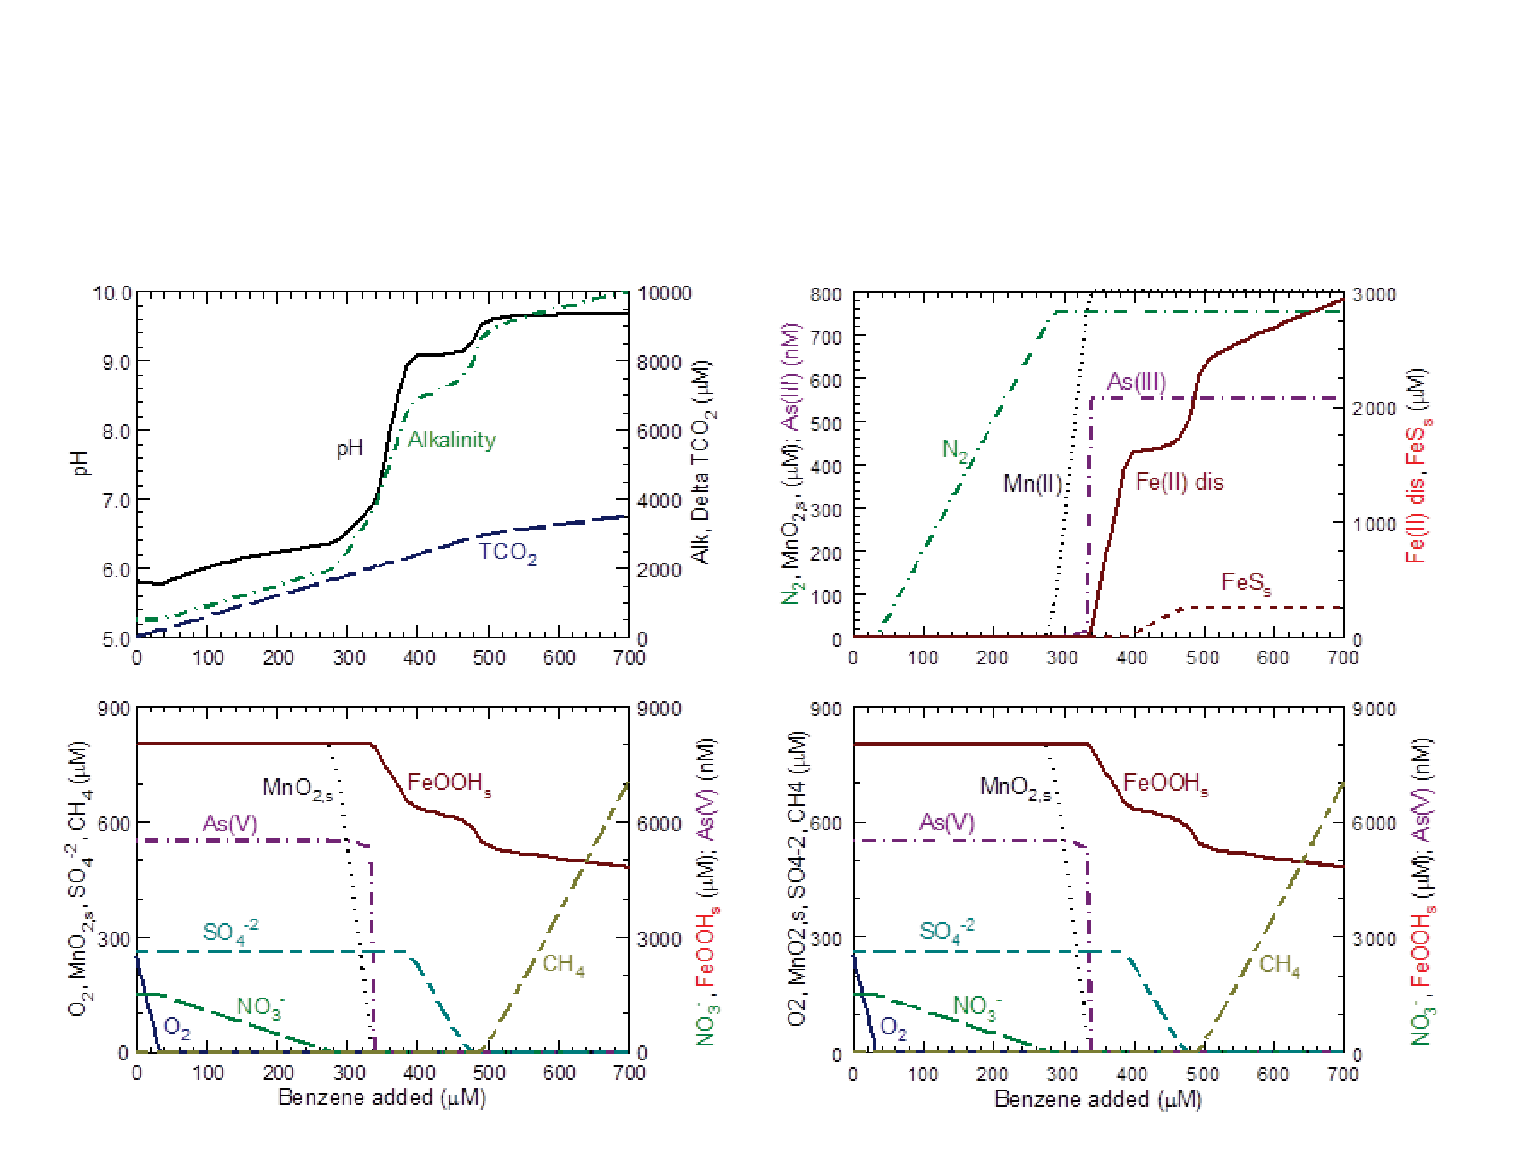
\includegraphics[width=1.0\textwidth]{redox_figure}
\caption[Results of the redox titration simulation.]{Results of the redox titration simulation.}
\label{fig:redox_titration}
\end{figure}








 

 



\chapter{Surface complexation reactions}
\def\shorttitle{Surface complexation reactions} % Abbreviated chapter title for right top header

\section{Background}


Oxides, hydroxides and organic matter carry functional groups at their surface, 
which  enable them to sorb cations, anions, and neutral species from solution.  
Typically, these functional groups behave as Bronsted acids and/or bases, 
which is to say they can accept hydrogen ions, release hydrogen ions, or, 
in some cases, both. The sorption behaviour depends on the type 
of mineral, crystal morphology, even which crystal face(s) dominate, 
as well as the composition and pH of the solution.
In response to uptake/release of hydrogen or other ions from/to solution, 
a net charge on the surface develops.

It can be shown that for a dissociation reaction (Appelo and Postma, 2005):
\begin{equation}
\log K_{\text{a}} = \log K_{\text{int}} + \frac{zF\psi_0}{RT \ln 10}
\end{equation}
in which $K_{\text{a}}$ is the apparent dissociation constant, $K_{\text{int}}$ is the intrinsic dissociation constant, $z$ is the charge of the ion, $F$ the Faraday constant (96,485 C/mol), $\psi_0$ the potential at the surface, $R$ the gas constant (8.314 J/K/mol) and $T$ the absolute temperature.

The intrinsic dissociation constant, $K_{\text{int}}$, applies to the chemical binding of the ion and the surface. The PRHEEQC database contains a compilation by Dzombak and Morel (1990) of laboratory-determined values of intrinsic dissociation constants for hydrous ferric oxide.

The apparent dissociation `constant' ($K_{\text{a}}$), however, varies with the potential and thus the charge at the surface. In order to calculate the $K_{\text{a}}$, the $\psi_0$ needs to be known. PHREEQC uses a double-layer model to relate the charge density on the surface ($\sigma_s$) with ionic strength ($I$, equation \ref{eq:ionic_strength}) and $\psi_0$ \citep{phreeqc2}.

\section{PHREEQC Exercise 5: Surface complexation reactions}
\subsection{Calculation of a charged surface composition}
This exercise demonstrates the use of the \textbf{SURFACE} keyword, which is used in PHREEQC for surface complexation calculations. The input file has already been prepared and is called {\color{red}kd\_surf.phrq}. The definition of the surface is as follows:

\begin{quote}
	SURFACE 1 \\
	Hfo\_w	2e-4	600	0.088 \\
	Hfo\_s	5e-6 \\
	-equilibrate 1 
\end{quote}

The names {\color{red}Hfo\_w} and {\color{red}Hfo\_s} correspond to the names of the master species in the PRHEEQC database that refer to the weak- and the strong surface sites, respectively. The number that follows is the number of surface sites in moles. For the weak sites, the surface area (600 m$^2$/g) and mass of ferrihydrite (88 mg) are also specified. Unless these values are explicitly typed for Hfo\_s as well, they apply to both the weak and the strong sites.

The input file contains BASIC statements that control the output to a text file in spreadsheet format. The distribution coefficient of Zn is calculated for both the weak and the strong sites, as well as an overall distribution coefficient. The file is called {\color{red}kd\_surf.prn} and can be opened in the Grid tab of PRHEEQC for Windows after the calculation has finished.

What is the value of the overall distribution coefficient for Zn? 

Answer: $K_d$ = \ldots\ldots.

Test the effect on the $K_d$ of:

\begin{itemize}

\item doubling the Zn concentration? Answer: $K_d$ = \ldots\ldots.

\item doubling the Mg concentration? Answer: $K_d$ = \ldots\ldots.

\item doubling the amount of ferrihydrite? Answer: $K_d$ = \ldots\ldots.

\item changing pH from 7 to 5? Answer: $K_d$ = \ldots\ldots.

\end{itemize}

\subsection{Uranium sorption at the Hanford site}

This exercise is based on uranium sorption over the range of chemical 
conditions at the Hanford 300 area in Richland, Washington, United States.  
You will simulate uranium sorption on hydrous ferric oxide under three 
sets of chemical conditions: groundwater with a large Columbia River signal, 
Hanford groundwater with moderate $Ca$ concentrations, 
and Hanford groundwater with high $Ca$.

Use the provided input file template to construct the 
input file ({\color{red}\textbf{SCM\_Exercise\_Template.xlsx}}).  
The template has the thermodynamic data for $Ca$- and $Mg-U(6)-CO3-2$ solution species.  
It also has thermodynamic data for the $U(6)$ sorption on hydrous ferric 
oxide from \cite{mahoney_2009}, 
who fit the best available data for $U(6)$ sorption 
on hydrous ferric oxide in the presence and absence of 
$CO_2$ using the thermodynamic data from the Wateq4f database.  

The simulation is based on the following set of laboratory batch experiments
\begin{itemize}
\item Equilibrate hydrous ferric oxide with {\color{red}\textbf{Groundwater 2}} that does not have uranium;
\item React the equilibrated hydrous ferric oxide with {\color{red}\textbf{River}} 
composition, which represents groundwater with a large Columbia River signal;
\item React the equilibrated hydrous ferric oxide with {\color{red}\textbf{Groundwater 1}} 
composition, which represents groundwater from the Hanford formation with moderate Ca concentration;
\item React the equilibrated hydrous ferric oxide with {\color{red}\textbf{Groundwater 2}} 
composition, which represents groundwater from the Hanford formation with high $Ca$.
\item Enter the solution composition for {\color{red}\textbf{Groundwater 2}} 
but without $U(6)$ under {\color{red}\textbf{SOLUTION 1}}.  
This will be used to equilibrate the hydrous ferric oxide before reacting 
with $U(6)$-containing groundwater compositions.  
Enter the compositions of the three groundwater datasets from 
Table \ref{tab:hanford1}
under {\color{red}\textbf{SOLUTION 10}}, 
{\color{red}\textbf{SOLUTION 50}}, 
and {\color{red}\textbf{SOLUTION 55}}, respectively.  
\end{itemize} 

\begin{table}[h]
\begin{center}
\centering
\caption{Groundwater compositions for the Hanford surface complexation exercise}
\begin{tabular}{cllll}
\toprule
Parameter  	& River	& Groundwater 1	& Groundwater 2	& Units/comment \\
pH	        & 6.00	& 8.11	        & 8.11	        & NIST/Fix \\
Temperature	& 21	  & 21	          & 21	          & $^\circ$C  \\
Alkalinity	& 0.164	& 5.00	        & 5.00	        & mmol/L \\
Na	        & 3.9	  & 6.8	          & 6.8	          & mmol/L \\
K	          & 0.15	& 0.2	          & 0.2	          & mmol/L \\
Mg	        & 0.5	  & 0.4	          & 0.4	          & mmol/L \\
Ca	        & 0.5	  & 0.5	          & 5.5	          & mmol/L \\
Cl	        & 1.49	& 1	            & 11	          & mmol/L charge \\
S(6)	      & 2.2	  & 1.4	          & 1.4	          & mmol/L \\
N(5)	      & 0	    & 0	            & 0	            & mmol/L \\
U(6)	      & 0.001	& 0.001	        & 0.001	        & mmol/L \\
\bottomrule
\end{tabular}
\label{tab:hanford1}
\end{center}
\end{table}

The keyword used for entering data for the surface assemblage is {\color{red}\textbf{SURFACE n}}.  
The required information is the name of the site, the moles of that site, 
the specific surface area (m2/g) of the solid, and the number of 
grams of the solid in the simulation.  
The specific surface area (SSA) and grams of solid (grams) 
are needed for calculating the coulombic term in the diffuse layer model.  
Under the {\color{red}\textbf{SURFACE 1}} keyword, 
enter the required data, which are in Table \ref{tab:hanford2}.

\begin{quote}
{\color{red}SURFACE 1} \\
\# Site	moles	SSA	grams \\
\end{quote}

\begin{table}[h]
\begin{center}
\centering
\caption{Concentrations of sorption sites and other data required for simulating surface complexation for this exercise}
\begin{tabular}{clll}
\toprule
Site name	& Moles of site              	& SSA (m2/g)	& Grams of HFO \\
Hfo\_s	  & 5.62 $times$ 10$^{-6}$	    & 600	        & 0.10 \\
Hfo\_w	  & 2.25 $times$ 10$^{-4}$	    & 600       	& 0.10 \\
\bottomrule
\end{tabular}
\label{tab:hanford2}
\end{center}
\end{table}

Below the section where the groundwater 
compositions and surface assemblage data are entered 
is a datablock to create a user-defined
{\color{red}\textbf{SELECTED\_OUTPUT}} file.  
This file simplifies determining the simulated sorbed $U(6)$ 
under the three sets of chemical conditions.

Below the {\color{red}\textbf{SELECTED\_OUTPUT}} file block, 
run the simulation. Using the {\color{red}\textbf{USE SURFACE 1}} 
and {\color{red}\textbf{USE SOLUTION n}} keywords 
(followed by an {\color{red}\textbf{END}} statement), 
react the equilibrated surface assemblage with the river-dominated groundwater, 
the Hanford aquifer groundwater with moderate $Ca$, 
and the Hanford groundwater with high $Ca$. 

The {\color{red}\textbf{SELECTED\_OUTPUT}} file will be written in the directory with the input file.  
Open the {\color{red}\textbf{SELECTED\_OUTPUT}} file 
with Excel and answer the following questions.

\begin{itemize}
\item What is the concentration of dissolved $U$, sorbed $U$, 
and percent of the total $U$ sorbed under each of set of conditions ?  
\item How did the pH change during reaction with of the surface assemblage with each of the groundwater compositions ?
\end{itemize}
\section[PHT3D Exercise 6, Zinc transport at the Cape Cod site]{PHT3D Exercise 6, Zinc transport at the Cape Cod site}

In this exercise we will construct a model that provides 
a good example for the consideration of surface complexation reactions in PHT3D.
The example is based on a modelling study for the Cape Code site, 
The full details of this study were reported in \cite{Kent20003411}.    
The Cape Cod research site is near a wastewater-treatment facility at 
the Massachusetts Military Reservation (MMR). A treated-sewage plume originated 
from the facility's infiltration beds, which were used from about 1936 to 1995. 
At the time the modelling study was undertaken the plume at the site extended 
more than 6 kilometers from the disposal site in the 
sand and gravel aquifer. The plume contains a complex mixture of phosphate, nitrate, 
metal ions (such as zinc), detergents, organic chemicals, and microbes. 
Over many years the plume and adjacent parts of the aquifer  
served as a field laboratory for a multidisciplinary team of scientists 
who investigated many fundamantal aspects 
of contaminant transport behaviour.

\subsection{Background: Groundwater Flow}

At the Cape Cod site the regional groundwater flow is generally towards 
the south, but locally the flow direction is directed from the 
sewage treatment facility towards the eastern shore of Ashumet Pond.  
The groundwater flow is nearly horizontal.
Approximately 25 cm/yr of areal recharge results
in a small vertical component to flow as well as
in the accumulation of a lens of pristine groundwater on top of 
the sewage plume, the thickness of which increases with 
distance away from the sewage 
treatment plant \citep[]{Leblanc1984,Leblanc1991895}.  
The magnitude of the hydraulic gradient 
is approximately 1.7 m/km. 
Seasonal fluctuations in the flow system result in small 
variations (approximately 0.2 m/km) in the magnitude
of the gradient as well as in small annual fluctuation 
in flow direction.

\subsection{Background: Hydrogeochemistry}

Contrasting chemical conditions between sewage-contaminated
and ambient groundwater gave rise to longitudinal and 
vertical gradients in groundwater chemistry. 
The ambient groundwater surrounding the sewage plume had 
high concentrations of dissolved oxygen, pH values 
in the range 5.3-5.8, and low concentrations of dissolved salts 
\citep[]{Leblanc1991895,Hess1996,Kent1999293}.
%[LeBlanc  et  al., 1991; Hess  et al., 1996; Kent and Maeder, 1999].
Sewage-contaminated groundwater under the disposal beds had high 
concentrations of nitrate.
Concentrations of dissolved oxygen successively decreased with depth 
\citep[]{Smith1991285,Smith19911815}.
%[Smith et al., 1991a].  
Biodegradation of organic matter in conjunction with solute transport 
away from the disposal beds resulted in the depletion of dissolved oxygen 
throughout the plume and the depletion of nitrate, followed by 
the accumulation of dissolved Fe(II), in the core of the plume 
%[Smith et al., 1991b; Kent  et  al., 1994]
\citep[]{Smith1991285,Kent19941099}. 
 
These biodegradation reactions influenced the pH  
within the aquifer zone affected by the sewage plume 
%[Abrams et al., 1998; Abrams and Loague, 2000b].
\citep[]{Abrams19981531,Abrams20002015}.
The principal chemical process in terms of controlling Zn transport is 
assumed to be Zn adsorption onto the sediments.
A single reaction with the stoichiometry could already adequately 
describe the pH effect observed in laboratory batch studies of
Zn adsorption onto the sediments \citep[]{Davis19982820}:

\begin{equation}
Zn^{2+}  +  >SOH    =  >SOZn^+  + H^+,  log  ^SQ_{SOZn}  
\label{eq:zn_single_site}
\end{equation} 

Adding a second surface site with the same reaction stoichiometry results in an  
SCM that can fit both the pH and Zn-concentration 
effect \citep[]{Davis19982820}.
This so-called two-site approach was one of the various
numerical implementations tested by \cite{Kent20003411}.
This two-site model will be used in the present exercise.
In the two-site SCM a small percentage of the total 
adsorption sites are considered to have a much greater affinity 
for adsorption ("strong sites," $>SsOH$) than the rest of the 
sites ("weak  sites," $>SwOH$): 

\begin{equation}
Zn^{2+}  +  >S_sOH    =  >S_sOZn^+  + H^+,  log  ^SQ_{S_sOZn}  
\label{eq:zn_strong_sites}
\end{equation} 

\begin{equation}
Zn^{2+}  +  >S_wOH  =  >S_wOZn^+  + H^+,  log  ^SQ_{S_wOZn}   \\
\label{eq:zn_weak_sites}
\end{equation} 

Before proceeding, it is worthwhile to consider the standard state for sorbed species 
in surface complexation models. 
The same standard state used for aqueous species - either 1 mole of surface complex \textbackslash L of solution (M)or \textbackslash kilogram water (m) - is often used for surface complexes as well. For example, the comprehensive compilation of equilibrium constants for sorption on hydrous ferric oxide by \cite{Dzombak1990} adopts a standard state of 1 M for sorbed species.  
One should be aware, however, there is a pitfall associated with this choice of 
standard state %\citet{appelo_postma_1999})
\citep[e.g.,][]{appelo_postma_1999}. 
The pitfall can be illustrated by considering a batch reactor with a suspension in sorptive equilibrium. 
In this thought experiment, we allow all of the solids to settle to the bottom of 
the reactor once sorptive equilibrium has been achieved, then we remove half of the solution without removing any solid.
Sorbed concentrations expressed in moles/kg water have now increased by a factor of two because the volume of solution (hence, mass of water) 
has decreased by a factor of two with no change in the amount of the solid.  
For surface complexation reactions such as those described the Eqn. \ref{eq:zn_strong_sites} 
and Eqn. \ref{eq:zn_weak_sites}, 
the concentration of sorbed Zn doubles and the concentration of free surface functional groups double,
so the factor of two cancels out in the mass action expression.  
For this type of surface complex - 
called ''monodentate'' (one surface site per sorbed species) -
the choice of standard state for sorbed species does not affect the value of the equilibrium constant. 
However, for ''bidentate'' surface complexes, where there are two surface functional groups 
bound to a single sorbing species, the situation is more complicated.  
Consider formation of a bidentate surface complexation analogous 
to Eqn. \ref{eq:zn_strong_sites}:

\begin{equation}
Zn^{2+}  +  2>S_sOH    =  (>SsO)2Zn + 2H^+  \\
\label{eq:zn_2}
\end{equation}

The mass action expression can be written with the concentration 
of the Zn surface complex raised to
the first power in the numerator and concentration of free surface 
sites squared in the denominator.  
In this mass action expression, the factor of two does not cancel out.  
This observation can be generalized by stating that equilibrium constants describing sorption where multidentate surface complexes are involved are a function of the solid to liquid ratio if a standard
state of 1 M or 1 m is adopted for sorbed species.  
There has been much discussion of this in the literature %(e.g.,\citet{wang_giammar_2013})
\citep[e.g.,][]{wang_giammar_2013}.  
To avoid this pitfall, PHREEQC adopts a standard state for sorbed species whereby the fraction 
of sites occupied by a given sorbed species equals 1.
In reaction \ref{eq:zn_2}, the relationship between sorbed Zn 
in units of moles \textbackslash kg water and 
sorbed Zn in units of mole fraction occupied 
sites is 
\begin{equation}
XZn = 2[(>SsO)2Zn]/[SsOHT],  \\
\label{eq:xzn}
\end{equation}
where square brackets refer to concentrations in moles/kg water and SsOHT is the total 
concentration of strong sorption sites.  
The factor of two results from the fact that the surface complex covers two sites.  
Therefore, when using equilibrium constants for multidentate sorbed species taken 
from the literature in a transport simulation, it is important to insure 
that either the equilibrium constant uses mole fraction of sites occupied 
by any given sorbed species = 1 or is properly converted to that standard state.  
Formulas for making such conversions are presented 
in various papers 
%\citep[see][]{jon90} 	    -->    	(see Jones et al., 1990)
\citep[e.g.,][]{wang_giammar_2013}.

\par With the sorption and thus the mobility of Zn being strongly 
depedent on pH, it is important to accurately capture the pH-controlling 
processes. For the vertical transect model that will be constructed
in this exercise the evolution of the pH will mostly be 
affected by (i) the transport and mixing of two different water 
types, i.e., of the (upstream) water composition
and the slightly more acidic (pH = 5.6) groundwater recharge water and (ii)
the pH increase that is induced by the degradation of organic matter
in conjunction with sulfate and iron reduction. The former causes
a pH gradient that is the result of physical transport processes. 
The latter causes inside the plume-affected aquifer zone
a pH increase towards 6.5, and thus above the 
pH of 6.0 that characterises the uncontaminated background water. 
For this exercise the organic matter degradation 
is represented in a simplistic way by a single kinetically 
controlled degradation reaction of DOC in conjunction
with the reduction of two electron acceptors sulfate and goethite.
It is assumed that nitrate is already depleted at the model's 
upstream boundary and thus not considered.
The rate $r_{DOC}$ of the DOC mineralisation is computed from:

\begin{equation}
r_{DOC} = \frac{C_{DOC}}{K_{DOC} + C_{DOC}} \sum_{i=1,nr_{EA}}{k_{EA_i} \frac{C_{EA_i}}{K_{EA_i} + C_{EA_i}}} 
\label{eq:doc_deg}
\end{equation}

where $C_{DOC}$ is the DOC concentration, $C_{EA_i}$ is the concentration of the $i^{th}$
electron acceptor (in the present case either sulfate or goethite) while $K_{DOC}$ and $K_{EA_i}$
are half saturation constants for DOC and the $i^{th}$
electron acceptor, respectively.

\par In reality the composition of the sewage plume and the 
reactions are obviously far more complex, as discussed in 
detail by \cite{Kent20003411}.
Nevertheless, the inclusion of this reaction allows to replicate
some of the key features observed at the site, and, most importantly,
allows to mimic the observed pH patterns relatively well.
Therefore the model constructed in this exercise also reproduces
the major Zn transport patterns relatively well, i.e., the rates 
of Zn movement and the vertical differences in the mobility, as induced
by the spatial variability of the pH.  

\begin{table}[hb]
\caption{Flow and solute transport parameters used for the setup of PHT3D Exercise 5}
\begin{center}
\begin{tabular}{lc} 
\toprule
Parameter                                            &         Value \\
\midrule
Flow simulation type                                 &  steady state  \\
Simulation time (days)                               &  21000         \\
Time step (days)                                     &  60            \\
Model \  extent\ column\ direction\ $ (m)$           &  400           \\
Model \ top\ elevation\ $(m)$                        &   16           \\
Model \ bottom\ elevation\ $(m)$                     &   0            \\
Horizontal hydraulic conductivity\ $(m/day)$         &   110          \\ 
Porosity, $\theta$                                   &   0.39         \\
Piezometric head downstream boundary\ $(m) $         &  14            \\ 
Longitudinal dispersivity, $\alpha_L$   $(m)$        &   1.0          \\
Horizontal transverse dispersivity, $\alpha_{TH}$    &   0.1          \\
Vertical transverse dispersivity,   $\alpha_{TV}$    &   0.01         \\
Effective diffusion coefficient, D$^{\star}$         &   0            \\
\bottomrule

\end{tabular}
\label{cape_cod_table_1}
\end{center}
\end{table}

\subsection{Setting up the flow model}

To set up the flow model proceed as follows:

\begin{itemize}

\item In ORTI, create a new model and save it in a new and separate directory (folder).

\item Select {\color{blue}Parameters} $\rightarrow$ {\color{blue}1.Model} 
$\rightarrow$ {\color{blue}Model} to specify the model dimension {\color{blue}('Xsection')}
and type {\color{blue}('unconfined')}

\item Select {\color{blue}Parameters} $\rightarrow$ 
{\color{blue}1.Model} $\rightarrow$ 
{\color{blue}Domain} to specify the domain as described in Table 
\ref{cape_cod_table_1}. 
For the first simulation select a spacing of 20 m in 
x direction and 1 m in y direction

\item Select {\color{blue}Parameters} $\rightarrow$ {\color{blue}Time} 
$\rightarrow$ and set the {\color{blue}Total Simulation Time} 
to 21000 days. Then define the step size to 60 days

\item Set the boundary conditions for heads by selecting 
{\color{blue}Spatial Attributes} $\rightarrow$ {\color{blue}MODFLOW} 
$\rightarrow$ {\color{blue}bas.3 Boundary Conditions} corresponding to
IBOUND (Modflow). 
Use the {\color{blue}Zone Tool} to create a zone at the 
outflow end that extends vertically between z = 0 m and z = 13.9 m.

\item To fix the hydraulic heads at the boundaries, use 
{\color{blue}Spatial Attributes} $\rightarrow$ 
{\color{blue}MODFLOW} $\rightarrow$ {\color{blue}bas.5 Initial Heads} and provide 
a value of 16 in the dialog box. This value will be used everywhere as a 
starting (initial) head and will be kept at this value at all locations
where a fixed head boundary condition was defined in the previous step. 
In order to fix the heads at the outflow boundary, 
draw a line at the same location as the outflow BC 
and attribute a head value of 14 m.

\item The inflow boundary is implemented by a single well that vertically extends 
between 0 and 15 m. The total injection rate of this well should be set to 2.16 $m^3/d$.

\item Select {\color{blue}Parameters} $\rightarrow$ {\color{blue}2.Flow} 
$\rightarrow$ {\color{blue}Parameters} 
and use this dialog to set several parametters. 
In {\color{blue}lpf.2} select {\color{blue}Convertible} 
for the {\color{blue}type of layer}. 
Then use {\color{blue}lpf.8} to specify the hydraulic conductivity.

\item To fix recharge, use {\color{blue}Spatial Attributes} $\rightarrow$ 
{\color{blue}MODFLOW} $\rightarrow$ {\color{blue}rch.2 Recharge}. 
Create a zone along the top cells and define a value of 0.0014 in the dialog box.

\item To define the porosity select {\color{blue}Spatial Attributes} 
$\rightarrow$ {\color{blue}MT3DMS} $\rightarrow$ {\color{blue}btn.11} and 
set {\color{blue}Value} to 0.39. 

\end{itemize}

Regularely save the changes to avoid loss of your data input.

\subsection{Running MODFLOW}

You have now completed the set up the flow model and are ready to run MODFLOW.
This step will provide PHT3D with the flow field that will be used to simulate 
reactive transport.

\begin{itemize}

\item Select {\color{blue}Parameters} $\rightarrow$ {\color{blue}2.Flow} $\rightarrow$ {\color{blue}Write}

\item Select {\color{blue}Parameters} $\rightarrow$ {\color{blue}2.Flow} $\rightarrow$ {\color{blue}Run}

\item When the calculations have finished, a new window will appear. I will show the last line(s) of the MODFLOW output file. Make sure MODFLOW terminated without errors.

\end{itemize}

\subsection{Visualising hydraulic heads}

\begin{itemize}

\item Visualise results by selecting {\color{blue}Results} $\rightarrow$ {\color{blue}2.Flow} $\rightarrow$ {\color{blue}Head}. The time step can be changed
in {\color{blue}Results} $\rightarrow$ {\color{blue}1.Model} $\rightarrow$ {\color{blue}Time}.

\item Assess if the head distribution is plausible.

\end{itemize}

\subsection{Chemistry}

In this section we will define (i) the initial hydrochemical 
composition (ii) the solutions that represent the sewage
plume composition at the upstream model boundary
and (iii) the groundwater recharge composition. 
Proceed with the following steps:

\begin{itemize}

\item Import the database from the folder that contains the Supporting Information for this exercise


\item The species needed to be activated are $Cl$, $C(4)$, 
$Fe(2)$ and $Fe(3)$, $Na$, $O(0)$, $S(-2)$ and $S(6)$, $Orgc$, $Zn$ and, as always, $pH$ and $pe$. 
As described in the previous PHT3D Examples, the activation of these species/componenets 
and the definition of the solution compositions are done in the {\color{blue}Solution Tab}. 
All required concentrations are listed in Table \ref{scm_solution_table}.

\item In is assumed that goethite is present at a (background) concentration 0.1 $mol/L_b$. 
FeS(ppt) must also be ticked. It is initially not present and thus the concentration
is left at the default value of 0.

\item The allocation of the solutions to define initial and boundary conditions
can be done via {\color{blue}ph.4 Source / Sink} zones (line). 
To allocate the correct solutions at the inflow boundary allocate 
from 14 m to 16 m $Solution\ 2$, from 3 m to 14 m 
allocate $Solution\ 1$ and between 0 m and 3 m allocate the background solution,
i.e., $Solution\ 0$.

\item The groundwater recharge composition is entered via {\color{blue}ph.5} as a line along 
the top grid cells. The recharge water composition is defined by $Solution\ 3$.
However, make sure that the recharge does not extend to the cell at the inflow end of the grid.   

\item Under the {\color{blue}Rates Tab} specify the degradation rate 
parameters for Orgc (0,1e-11, 1e-12, 1e-12,1e-17,1e-17 respectively) and also 
enter the stoichiometry of the mineralisation 
reaction. The formula is 
Orgc -1.0 CH2O 1.0.
%Orgc -1.0 CH2O(NH3)0.15 1.0.

\item Activate both available types of surface sites, i.e., $S\_s$ and $S\_w$.
Define 1.59e-5 $mol/L_b$ and .0018 $mol/L_b$ as their respective background concentrations.


\end{itemize}

\subsection[Running PHT3D]{Running PHT3D}

With the model setup completed run PHT3D and visualise the results via contour plots.


\begin{table}[hb]
\caption{Chemical composition for PHT3D Exercise 5}
\begin{center}
\begin{tabular}{lcccc} 
\toprule
Parameter  & Background & Solution 1 & Solution 2 & Solution 3\\
\midrule
C(4)      &   1e-4 &   1e-4  &   1e-4 &   1e-4\\
Cl      &   0 &   0  &  0  &   1e-4 \\
Fe(2)      &   0 &   0  &  0  &   0 \\
Fe(3)      &   0 &   0  &  0  &   0 \\
Na      &   2.3e-4 &   2.3e-4 &   2.3e-4 &   3.13e-4 \\
O(0)      &   5e-4 &   0 &   5e-4 &   5e-4\\
Orgc      &   0 &   1e-4 &   0  &  0 \\
S(6)      &   1e-4 &   1e-4  &   1e-4 &   1e-4\\
S(-2)      &   0 &   0  &  0  &   0 \\
Zn      &   0 &   8e-6  &  8e-6  &   0 \\
pH      &   6 &   6 &  6  &   5.6 \\
pe      &   14.6 &   4 &  14.6  &   14.2 \\
\bottomrule

\end{tabular}
\label{scm_solution_table}
\end{center}
\end{table}


\include{scm/dd_u_ipht3d_final}
%\section[PHREEQC Exercise 5: Site-specific surface complexation model for As]{PHREEQC Exercise 5: Site-specific surface complexation model for As}

In this exercise, we will use PHREEQC to develop a model that can quantitatively describe
the site-specific sorption characteristics of natural sediment material collected from a 
Pleistocene aquifer near Hanoi, Vietnam. This can be done by formulating a set of surface reactions and by adjusting 
the log\_ks of those reactions until they match the experimental data that were
collected from anaerobic laboratory batch experiments. Even though this example is 
focused on arsenic, the procedure itself is more generally applicable to a wide range of metals amd metalloids.
Both the sorption experiments and the SCM development for the Pleistocene sands are described 
in more detail by \cite{rathi2017a}. 
The measured data suggest that $As(III)$ sorption on the sediments increased non-linearly and phosphate ions competed strongly with $As(III)$ for adsorption. 
The SCM employed to describe these data is a generalized composite model, as proposed by \cite{Davis19982820}. 
In this approach a generic surface site ({\color{blue}Site\_sOH}) is thought to be responsible for adsorption 
of both $As(III)$ and $PO_4-P$. Note, that these modelled sites are not associated with a particular mineral phase of the Pleistocene sediments but represent the overall sorption behaviour of the entire mineral assemblage. 

\begin{table}[h]
\caption{Adjustable parameters, including surface complexation reaction constants 
for $As$ and sorption site density.}
\begin{center}
\begin{tabular}{l c}
\hline
 Reaction / Parameter & Best value          \\ \hline
$Site\_sOH$ + $As\_threeO_3^{3-}$ + 3$H^+$ = $Site\_sH_2As\_threeO_3$   + $H_2O$  & 43.665 \\
$Site\_sOH$ + $As\_threeO_3^{3-}$ + 2$H^+$ = $Site\_sHAs\_threeO_3^{-}$ + $H_2O$	&  ? \\
$Site\_sOH$ + $PO_4^{3-}$ + 3$H^+$         = $Site\_sH_2PO_4$           + $H_2O$	&   31.281 \\
$Site\_sOH$ + $PO_4^{3-}$ + 2$H^+$         = $Site\_sHPO_4^-$           + $H_2O$	&  29.065 \\
$Site\_sOH$ + $PO_4^{3-}$ + $H^+$          = $Site\_sPO_4^{2-}$         + $H_2O$	&  15.393   \\
$Site\ density$	& ? \\ \hline
\end{tabular}
\label{ex_as_scm}
\end{center}
\end{table}

The PHREEQC input file {\color{red}as\_scm\_wrr2017.phrq} that controls the model simulations 
and the two files containing experimental data ({\color{red}as\_iso.tsv for $As(III)$} 
and {\color{red}as\_po4.tsv} for $PO_4$)
have been prepared for you. \\

\begin{quote}
{\color{blue}\textbf{SURFACE 1}} \\
{\color{blue}\textbf{Site\_sOH .... \#enter value\#}}\\ 
{\color{blue}\textbf{-no\_edl}}\\
{\color{blue}\textbf{END}}\
\end{quote}

As can be seen, the model uses the {\color{blue}\textbf{no\_edl}} 
option, which means that the surface complexation reactions
do not consider any electric double layer effects.

%Since, the charge density on the surface (σs) of the sediments is difficult to measure, 
% we cannot estimate the intrinsic dissociation constant in reaction 5.1. 
%The model uses the nothe SURFACE keyword in PHREEQC was defined with no_edl term: 

Using the {\color{blue}\textbf{no\_edl}} mode, no input is required for surface area and sorbent mass. 
It is important to note, that the unit of surface site density is moles of sites per litre of solution.
Each individual laboratory batch sorption experiment is simulated in PHREEQC 
as a batch reaction between the {\color{blue}\textbf{SURFACE}} and an aqueous 
{\color{blue}\textbf{SOLUTION}} for which the composition is changed
from experiment to experiment. $As(III)$ and $PO_4$ were added 
using the {\color{blue}\textbf{REACTION}} keyword while the naturally 
adsorbed concentrations of $As(III)$ and $PO_4$ were included in the initial 
solution using the {\color{blue}\textbf{SOLUTION}} and 
{\color{blue}\textbf{SOLUTION\_SPREAD}} keywords. 
The experimentally observed pH was fixed in the model 
using the {\color{blue}\textbf{EQUILIBRIUM\_PHASES}} keyword:\\

\begin{quote}
{\color{blue}\textbf{EQUILIBRIUM\_PHASES 1}} \\
{\color{blue}\textbf{Fix\_pH -6.30 HCl 10.0 }}\\
\end{quote}

where, {\color{blue}\textbf{Fix\_pH}} is defined in the {\color{blue}\textbf{DATABASE}} 
section of the model file as follows:\\

\begin{quote}
{\color{blue}\textbf{PHASES}}\\
{\color{blue}\textbf{Fix\_pH}} \\
{\color{blue}\textbf{H+ = H+}}\\ 	
{\color{blue}\textbf{log\_k	0 }}\\
\end{quote}

Finally, the {\color{blue}\textbf{USER\_GRAPH}} keyword is used to control 
the simultaneous plotting of the observation data and of 
simulation results. You can now play with this model and systematically
vary the values of two selected adjustable model parameters, i.e.,
\begin{itemize}
\item one of the three logKs for $As(III)$ (Hint: try logKs between 40 and 45)
\item surface site density for $Site\_sOH$ (Hint: try densities 
between 1 $\times$ $10^{-5}$ and 3 $\times$ $10^{-5}$)
\end{itemize}

Fill the values that achieve the best match with the observed data into Table \ref{ex_as_scm} .



\section[PHT3D Exercise 7: Incorporation of the site-specific SCM into a reactive transport model]{PHT3D Exercise 7: Incorporation of the site-specific SCM into a reactive transport model}

At the study site for which the above SCM was developed, Van Phuc, groundwater extraction near Hanoi and the resulting changes in hydraulic conditions have caused surface water from the Red River to infiltrate into the  adjacent Holocene aquifer and further into the laterally neighbouring Pleistocene aquifer. 
Associated with the changes in hydrologial conditions arsenic mobilisation at the interface 
between the Red River and the aquifer has caused an extensive arsenic plume at the site. 
However, while the mobility of $As$ in the Holocene aquifer is considered to be relatively high, 
$As$ transport within the Pleistocene section of the aquifer has been significantly retarded \citep{vangeen2013}. In this PHT3D exercise we use a simple 1-D reactive transport model to illustrate the effect of variable geochemical conditions on the extent of $As$ sorption, most importantly how competition between $PO_4$ and $As$ affects arsenic mobility. We will compare how the effective retardation factors that are obtained with these SCM-based models compared coefficients compare with the earlier suggested retardation factors of 16 to 20 \citep{vangeen2013}. 

For this exercise the model file {\color{blue}\textbf{as\_1d.orti}} and the corresponding database file {\color{blue}\textbf{pht3d\_datab.dat}} are provided as a base version. The model simulates groundwater flow over a 50-year period over a distance of 2,500 m. The conservative transport behaviour of the model can be seen from visualising the concentration of the species {\color{blue}\textbf{Tracer}} in the Transport Results section. This can be done by 

\begin{itemize}
\item  going to {\color{blue}Parameters} $\rightarrow$  {\color{blue}3. Transport} $\rightarrow$ {\color{blue}Spc}, specifying {\color{blue}Type} $\rightarrow$ {\color{blue}Mt3dms} and entering the word \textbf{Tracer} under {\color{blue}Species}. 

\item Then under {\color{blue}Parameters} $\rightarrow$ {\color{blue}3. Transport} $\rightarrow$ {\color{blue}P}, select {\color{blue}RCT} $\rightarrow$ {\color{blue}rct.1 – major flags} 
and enter {\color{blue}ISOTHM sorption} $\rightarrow$ no sorption. 

\item Now that we have defined a conservative tracer species, we will provide its concentration in {\color{blue}Spatial Attributes} $\rightarrow$ {\color{blue}Mt3dms} $\rightarrow$ {\color{blue}BTN} $\rightarrow$ {\color{blue}btn.13 Concentrations}. 

\item Use the point zone tool to add a tracer concentration of 1 in the 1st grid cell (x = 1.2m, y = 0.5m). Set the background boundary condition type to 1 in all grid cells. To do this 
go to {\color{blue}Spatial Attributes} $\rightarrow$ {\color{blue}Mt3dms} $\rightarrow$ {\color{blue}BTN} 
$\rightarrow$ {\color{blue}btn.12}. Boundary conditions $\rightarrow$ {\color{blue}Backg.}. 

\item Now write the model input files and run MT3DMS. 

\item You can now visualise the concentration profile of the tracer 
for the final time step (18250 days) under {\color{blue}Results} $\rightarrow$ {\color{blue}3. Tracer}.
\end{itemize}

In a first step we will reproduce the results of \cite{vangeen2013} by 
employing a linear sorption model for $As$ such that the proposed retardation factor of 16 is achieved. 

\begin{itemize}
\item Go to {\color{blue}Parameters} $\rightarrow$ {\color{blue} 3. Transport} $\rightarrow$ {\color{blue} Spc}, specify {\color{blue} Type} $\rightarrow$ {\color{blue} PHT3D} and enter {\color{blue}Species} $\rightarrow$ \textbf{$As\_three$}. 

\item Then under {\color{blue} Parameters} $\rightarrow$ {\color{blue} 3. Transport} $\rightarrow$ {\color{blue} P}, select {\color{blue} RCT} $\rightarrow$ {\color{blue} rct.1 – major flags} 
and enter {\color{blue} ISOTHM: sorption} $\rightarrow$ {\color{blue} linear}. 

\item Now, in {\color{blue} Parameters} $\rightarrow$ {\color{blue} 3. Transport} $\rightarrow$ {\color{blue} Rct}, enter a value of 1.7 for {\color{blue} SP1}, which represents the distribution coefficient Kd. 

\item Then, under {\color{blue}Spatial Attributes} $\rightarrow$ {\color{blue} Mt3dms} $\rightarrow$ 
{\color{blue} RCT} $\rightarrow$ {\color{blue} rct.2a bulk density} provide a {\color{blue}Background} 
value of 1.988 kg/l for all cells.

\item Now go to {\color{blue}Parameters} $\rightarrow$ {\color{blue} 4. Chemistry} and {\color{blue} import database}and the enter into Chemistry tab. 
\item You can see that different solution compositions have already been entered for you. 
Under {\color{blue}Spatial Attributes} $\rightarrow$ {\color{blue}Pht3d} $\rightarrow$ {\color{blue}ph.3 Initial chemistry} specify the {\color{blue}background} solution 0 and under {\color{blue}ph.4 Source/sink} use {\color{blue}add zone} to specify a source concentration for solution 1 in the 1st grid cell. 
\item Write the model input files and run PHT3D. 
\item Once the model execution is finished you can visualise the profile of $As\_three$ 
at time 18250 days under {\color{blue}Results} $\rightarrow$ {\color{blue} 5. Observations}. 
Similarly, you can reproduce a retardation factor of 20 by changing the {\color{blue}SP1} value to 2.1 l/kg.

\item Finally, to incorporate surface complexation model in the 1-D simulation, de-activate the {\color{blue}RCT} module of MT3DMS and specify the surface site density values for {\color{blue}Site\_s} under {\color{blue}Parameters} $\rightarrow$ {\color{blue}4. Chemistry} $\rightarrow$ {\color{blue}Surface} $\rightarrow$ {\color{blue}Site\_back}. 
Now write the model input files and run PHT3D. Then compare the $As\_three$ concentration profile with the profile obtained with the linear isotherm simulations. \\
\end{itemize}

What is the resulting retardation factor for $As$ in the SCM-based model ?



%\DeclareGraphicsExtensions{.png}
\chapter{Redox Reactions}
\def\shorttitle{Redox Reactions} 
\section[Background]{Background}

Understanding oxidation-reduction (redox) reactions that occur in natural 
and contaminated systems is central to developing accurate conceptual and 
quantitative models. Redox reactions involve the transfer of electrons 
between constituents and therefore, changes in the oxidation state of 
one or more elements. Changes in oxidation state of an element can 
result in dramatic changes in its chemical and physical properties.  
For example, iron in the plus three oxidation 
state - Fe(III) - in surficial deposits renders 
a reddish hew to Mars whereas iron in the plus II oxidation 
state - Fe(II) - in surficial basalts on the Moon is, in no 
small part, responsible for the blackness of the lunar mares. 
Two important examples of redox reactions are the oxidation 
of aqueous Fe(II) to Fe(III) or organic carbon by dissolved oxygen:

\begin{equation}
4Fe^{+2} + O_{2,aq} + 10H_2O \rightarrow 4Fe(OH)_{3,s} + 8H^+  \\
\label{eq:fe2_oxidation}
\end{equation}

\begin{equation}
CH_2O  + O_{2,aq} + 10H_2O \rightarrow CO_{2,aq} + H_2O \\
\label{eq:om_reduction}
\end{equation}

Rather than representing formaldehyde, $CH_2O$ is often used to represent 
one sixth of a glucose molecule.

The classical approach to discussing redox reactions in aqueous geochemistry 
is to split the redox reactions into two hypothetical 
half reactions involving electrons. 
Using this approach, reaction \ref{eq:fe2_oxidation} and \ref{eq:om_reduction} 
would be broken up into the following half reactions:

\begin{equation}
Fe^{+2} + 3H_2O  \rightarrow Fe(OH)_{3,s} + 3H^+ + e^-  \\
\label{eq:fe_half_reac}
\end{equation}

\begin{equation}
CH_2O + H_2O \rightarrow CO_{2,aq} + 4H^+ + 4e^-  \\                    
\label{eq:om_half_reac}
\end{equation}

\begin{equation}
O_{2,aq} + 4H^+ + 4e^-  \rightarrow 2H_2O \\
\label{eq:ox_half_reac}
\end{equation}

Mass action expressions are then written for the half reactions.
For example, for the Fe(II)/Fe(III) half reaction, 
the mass action expression is:

\begin{equation}
K = a_{Fe(OH)_{3,s}} a_{H^+}^3 a_{e^-}/a_{Fe}^{+2} a_{H_2O}^3 \\
\label{eq:rdx6}
\end{equation}

The standard state of the $e^-$ is the same as other aqueous species,
1 mole per kilogram water.  
This approach comes from the field of electrochemistry, where the oxidation and 
reduction half reactions can be made to occur in separate place
connected, for example, 
through a meter that measures the electromotive force (or power source) 
and a salt bridge.
In dilute solutions the activity of water can be equated with its mole fraction,
which is essentially 1. If pure ferric hydroxide forms then it 
can be assumed to be in 
its standard state (mole fraction $Fe(OH)_{3,s}$
equals 1), 
so Eqn (\ref{eq:rdx6}) can be re-written:

\begin{equation}
K=a_{H^+}^3 a_{e^-}/a_{{Fe}^{+2}} \\    
\label{eq:rdx7}
\end{equation}
                                                         
Taking the base-10 logarithm, \ref{eq:rdx7} becomes: 
\begin{equation}
logK = 3loga_{H^+} + loga_{e^-} -loga_{{Fe}^{+2}}  \\                          
\label{eq:rdx8}
\end{equation}

Analogous to the definition of $pH$,
$loga_{e^-}$
is defined as $pe$.
This formalism is useful for graphically representing the 
relative thermodynamic stability of redox-reactive species 
in natural and contaminated systems 
(typically in their standard state).

Electrochemists have established logK values for 
half reactions based on the 
convention that the hydrogen gas -
hydrogen ion half reaction
\begin{equation}
H_{2,g}  =  2H^+ + 2e^- \\   
\label{eq:rdx9}
\end{equation} 
has an electromotive force and, therefore a logK 
value of 0 for $H_{2,g}$ and $H^+$ in their 
standard states (1 atmosphere and 1 mol/kgw, respectively).  
Using this convention, logK values for half reactions can be assembled 
in order of thermodynamic favorability, 
called a redox ladder, such as Table \ref{tab:rdx1}.  
Note that the logK values apply to all species in their standard state 
(1 mol/kgw for aqueous species, pure solid phase activity 
equals 1, and 1 atmosphere for gasses).  
Also, the logK value for half reactions where solid phases are participants 
depends on the thermodynamic stability of the solid phase.  
For example, reduction of $ferrihydrite$ (fhy) is more favorable than 
reduction of $goethite$ (based on the logK values for goethite that 
applies to the Cape Cod aquifer, Kent et al., 2008) because $goethite$ 
is thermodynamically more stable than $ferrihydrite$.  
Plots of $pH$ against $pe$ constructed using reactions and logK values like 
those in Table \ref{tab:rdx1} are used to illustrate 
trends expected in redox processes 
with changes in pH. In the exercises that will follow below, 
we will explore these trends.

\begin{table}[h]
\topcaption{Half reactions and logK values for some redox-reactive species}
\centering
%\footnotesize
\begin{tabular}{rcll}
\toprule
Half reactions, per electron				  & &									                  & logK \\ \hline
0.25 $O_{2,aq}$ + $e^-$ + $H^+$       &=& $0.5H_2O$											    & 21.52 \\
0.2  $NO_3^-$ + $e^-$ + $1.2H^+$      &=& 0.1 $N_{2,aq}$ + 0.6 $H_2O $      & 20.71 \\
0.5 $MnO_2:H_2Os$ + $e-$ + $2H^+$     &=& $0.5Mn^{+2}$ + $1.5H_2O$				  & 20.69 \\
0.5 $HAsO_4^{-2}$ + $e^-$ + $2H^+$    &=&  0.5 $As(OH)_{3,aq}$ +  $0.5H_2O$	      & 19.80 \\
$FeOOH$ + $e^-$ + $3H^+$              &=& $Fe^{+2}$ + $2H_2O$  fhy							    & 17.91 \\
$FeOOH$ + $e^-$ + $3H^+$              &=& $Fe^{+2}$ + $2H_2O$  Goethite (Kent et al. 2008)	    & 13.52 \\
$0.125SO_4^{-2}$ + $e^-$ + $1.125H^+$ &=& $0.125HS^-$ + $0.5H_2O$							    & 4.21 \\
$0.125CO_3^{-2}$ + $1.25H^+$ + $e^-$  &=& $0.125CH_{4,aq}$ + $0.375H_2O$						& 5.13 \\
\bottomrule
\label{tab:rdx1}
\end{tabular}
\end{table}	

\begin{table}[h]
\topcaption{PHREEQC keywords for simulating redox equilibria}
\centering
\footnotesize
\begin{tabular}{llll}
\toprule
Constituents	& Database	                & Input	     & Selected\_Output   \\ \hline
Aqueous       &	SOLUTION\_MASTER\_SPECIES & SOLUTION n & Totals (e.g., Ca)   \\
              & SOLUTION\_SPECIES	        & MIX n      & Molalities (e.g., $Ca^{+2}$) \\
              &                           &            & Activities (e.g., $Ca^{+2}$) \\
              &                           &            & Saturation\_index  \\
              &                           &            & USER\_PUNCH       \\
              &                           &            &        SC         \\
              &                           &            &     Rho           \\
              &                           &            &   Soln\_Vol        \\ \hline
Gas phase	    & Phases	   & EQUILIBRIUM\_PHASES n   & EQUILIBRIUM\_PHASES \\
              &            &                         & USER\_PUNCH   \\
              &            &                         & EQUI(...)     \\ \hline
Solid phase	  & Phases     & EQUILIBRIUM\_PHASES n   & See Gas Phase \\ \hline
Surface       & SURFACE\_MASTER\_SPECIES & SURFACE n & See aqueous   \\
complexation  & SURFACE\_SPECIES         &           &       \\ \hline
Other         &                          &           &       \\ \hline
SAVE, USE	    & Solution n,              &           &       \\
              & EQUILIBRIUM\_PHASES n    &           &       \\ 
							& EXCHANGE  n              &           &       \\ 
							& SURFACE n                &           &       \\ \hline
REACTION n    &	Irreversible addition    &           &       \\
              & of compounds             &           &       \\ 

\bottomrule
\label{tab:keywords}
\end{tabular}
\end{table}	

\section[PHREEQC Exercise 6]{PHREEQC Exercise 6}

This series of exercises involves using PHREEQC to react 
oxidized and reduced species. As you will see, 
the oxidation reduction reactions 
also induce changes in pH and other secondary reactions.


\begin{table}[h]
\caption{Water compositions for the mixing exercise. Adjust Na to achieve charge balance for the oxic solution and Cl to achieve charge balance for the anoxic solution.}
\begin{center}
\begin{tabular}{lccc} 
\toprule
Parameter   & Oxic GW & Anoxic GW & Units  \\ \hline
pH          & 6.50 		& 6.50 			& -      \\
pe          & 12   		& 4    			& -      		\\
Temperature & 21   		& 21   			& $^\circ$C \\
Alkalinity  & 710  		& 710  			& $\mu$eq/L  		\\
Na          & 780  		& 580  			& $\mu$mol/L \\ 
K           & 8.0  		& 75   			& $\mu$mol/L \\
Mg          & 18.0 		& 53   			& $\mu$mol/L \\
Ca          & 9.0  		& 170  			& $\mu$mol/L \\ 
Cl          & 82   		& 550  			& $\mu$mol/L \\ 
S(6)        & 24.0 		& 100  			& $\mu$mol/L \\ 
O(0)        & 500  		& 0    			& $\mu$mol/L \\ 
Fe(2)       & 0    		& 179 			& $\mu$mol/L \\ 
\bottomrule
\end{tabular}
\label{tab:rdx2}
\end{center}
\end{table}

\subsection[Mixing-induced redox reactions]{Mixing-induced redox reactions}

\begin{itemize}
\item Set up two solutions, one with $O_2$ and one with $Fe(II)$, using the compositions in Table \ref{tab:rdx2}. {\color{red} \textbf{MIX}} them in equal proportions. (Keywords: {\color{red} \textbf{SOLUTION n}}, {\color{red} \textbf{SOLUTION m}}, {\color{red} \textbf{MIX o}}). The solutions begin with the same $pH$ and $alkalinity$. What about the $TCO_2$ concentration ? $TCO_2$ is the sum of the concentrations of all carbonate-containing aqueous species. 
	\begin{enumerate} 
	\item What happens to the $pH$, $alkalinity$, and $TCO_2$ concentrations after mixing ?
	\item What happens to the concentrations of $O_2$, $Fe(II)$, and $Fe(III)$ after mixing?  What are the dominant $Fe$ aqueous species ?
	\item What happens to the $PCO_2$ after mixing?
	\end{enumerate} 
\item Use the anoxic solution. Allow 10 umoles of $O_2(g)$ from the atmosphere ($PO_2$ = 0.2 atmospheres) to equilibrate with the solution. 
(Keyword: {\color{red} \textbf{EQUILIBRIUM\_PHASES n}}.)
  \begin{enumerate} 
	\item What happens to the $pH$, $alkalinity$, and $TCO_2$ concentrations after mixing ?
	\item What happens to the concentrations of $O_2$, $Fe(II)$, and $Fe(III)$ after mixing?  What are the dominant $Fe$ aqueous species?
	\item What happens to the $PCO_2$ after mixing?
  \end{enumerate}
\item Repeat the previous exercise where first 100 $\mu$moles then 1000 $\mu$moles of $O_2$ from the atmosphere equilibrate with the anoxic solution, but allow ferrihydrite ($Fe(OH)3(a)$) or goethite ($Goethite$) to precipitate until it reaches equilibrium.
	\begin{enumerate}  
	\item What happens to the $pH$, $alkalinity$, and $TCO_2$ concentrations after mixing ?
	\item What happens to the concentrations of $O_2$, $Fe(II)$, and $Fe(III)$ after mixing?  What are the dominant $Fe$ aqueous species ?
	\item What happens to the $PCO_2$ after mixing ?
	\item What happens when the solution is allowed to equilibrate with atmospheric $PCO_2$ ?
	\end{enumerate} 
\item Simulate reacting the oxic solution with 500 umoles of amorphous $FeS$ ($FeS(ppt)$) (ca. 44 mg) allowing $Fe(OH)3(a)$ to precipitate. 
	\begin{enumerate}  
	\item What got oxidized ? What did not get oxidized? What was the $pH$ ?
	\item Repeat the simulation, this time allowing the suspension to equilibrate with atmospheric $O_2$. What was the $pH$ ? What got oxidized ?
	\end{enumerate}  
\end{itemize} 


\subsection[Redox sequence]{Redox sequence}

The next exercise compares the standard sequence of oxidation- reduction reactions 
predicted using the redox ladder to the sequence in which oxidants (electron acceptors) 
actually get reduced by organic carbon based on thermodynamic considerations.   
The exercise uses the keyword {\color{red} \textbf{REACTION n}} to add $CH_2O$, 
which represents one six$^{th}$ of a glucose molecule, to a suspension with aqueous and solid-phase oxidants.  
As $CH_2O$ is added it reacts with the oxidants that are most thermodynamically favorable. 
Thermodynamic favorability depends on concentrations and solid-phase solubilities 
(which depend on $pH$ for some important oxidants).  
Thus the order in which the oxidants react with $CH_2O$ may change during the course 
of the redox titration as the chemical conditions change.  

\textbf{Note, that you will need to use either the {\color{red} \textbf{Wateq4f.dat}} 
or {\color{red} \textbf{Minteq.v4.dat}} database, 
because the Phreeqc.dat database does not include arsenic or uranium.}


\begin{itemize}
\item Create a PHREEQC input file and set up the initial solution and solid-phase compositions 
in the suspension using the data in Table \ref{tab:rdx3}.  
Assume the suspension has one kilogram of water.  
(Keywords: {\color{red} \textbf{SOLUTION n}}, {\color{red} \textbf{EQUILIBRIUM\_PHASE n}}).  
Adjust the chloride concentration to insure charge balance of the solution. 
Two solid phases with reduced species may precipitate if they become supersaturated: 
amorphous $FeS$ ($FeS(ppt)$ in Phreeqc) and $Siderite$.

\begin{table}[h]
\caption{The composition of the suspension used for the redox sequence and redox titration exercises}
\begin{center}
\begin{tabular}{lcc} 
\hline
	   & Value	 & Units \\
pH	 & 5.80	   & - \\
T 	 & 22	     & $^\circ$C \\
C(4) &	2514	 & $\mu$M \\
Na	 & 2580	   & $\mu$M \\
K	   & 330	   & $\mu$M \\
Mg	 & 170	   & $\mu$M \\
Ca	 & 570	   & $\mu$M \\
Cl	 & 1766	   & $\mu$M \\ 
Water	& 1	     & Kg = L \\ \hline % should be approx. not equal
Redox-reactive constituents & &\\ \hline
O2 	  & 250	      & $\mu$M \\
N(5)	& 1500	    & $\mu$M (use Nit not N) \\
Pyrolusite & 800	& $\mu$moles \\
As(5)      &	1	  & $\mu$M \\
U(6)	     &  1	  & $\mu$M \\
Fe(OH)3(a) or Goethite 	& 8000	& $\mu$moles \\
S(6) 	                  & 260	  & $\mu$M \\ \hline
\end{tabular}
\label{tab:rdx3}
\end{center}
\end{table}


Using thermodynamic data from the PHREEQC database 
(and the Wateq4f or Minteq.v4 database if arsenic or uranium are included), 
the redox ladder for the oxidized species in Table \ref{tab:rdx1} follows the sequence: 
$O_2$, $NO_3^-$, $MnO_2$ ($Pyrolusite$), $As(V)$, ferric hydroxide (ferrihydrite, $Fe(OH)3(a)$ 
in the PHREEQC database, or $Goethite$), and $SO_4^{-2}$ 
(Table \ref{tab:rdx1}).  
This sequence is based on all reactants in Table \ref{tab:rdx1} 
being in their standard state at $pH$ 7 and 25 $^\circ$C.  
Use the {\color{red} \textbf{SAVE}} keyword to save 
the composition of the solution and the equilibrium phase assemblage.

\item Use the keyword {\color{red} \textbf{USE}} to recall the compositions 
of the solution and equilibrium phase assemblage created previously.  
Use the {\color{red} \textbf{REACTION n}} keyword to add an increment of $CH_2O$.  
Try adding a suffiently large amount of $CH_2O$ to remove about half of the dissolved oxygen, 
then try again with a now sufficiently large amount of $CH_2O$ 
to remove all the dissolved oxygen and even some of the nitrate, etc.  
Examine the order in which oxidants get reduced. Any surprises ?

\item Using the keyword {\color{red} \textbf{SELECTED\_OUTPUT}}, 
set up a file that includes simulation data of interest to this exercise 
without a lot of the other information that, while interesting, 
clutters the most significant simulation results.  
Consult the manual under the {\color{red} \textbf{SELECTED\_OUTPUT}} 
keyword to have the following information sent to the selected output file: 
$pH$, $alkalinity$, concentrations of the total dissolved oxygen ($O(0)$), nitrate ($N(5)$), 
$Pyrolusite$, $As(5)$, ferric hydroxide ($Fe(OH)3(a)$ or $Goethite$, 
whichever you chose to use), $S(6)$, $Siderite$, and $FeS(ppt)$.  
For the solid phases, you can use the {\color{red} \textbf{-equilibrium\_phases}} 
list-of-phases command under {\color{red} \textbf{SELECTED\_OUTPUT}}.  
For each phase in the list, this will send the total number of moles 
remaining and the number of moles added (positive value) or removed (negative value) 
to the {\color{red} \textbf{selected output file}}.  
Alternatively, you can also add a {\color{red} \textbf{USER\_PUNCH}} 
list to your {\color{red} \textbf{SELECTED\_OUTPUT}}.  
Consult the PHREEQC manual under the {\color{red} \textbf{USER\_PUNCH}} keyword.  
It will explain how to add the appropriate heading.
To add the moles of a solid (or gas) phase, use 
{\color{red} \textbf{PUNCH Phases (phase name)}}, % shoul be Phases("`phase name”)
as explained in Table 8 of the PHREEQC manual.  
The selected output file (note, you should not forget to give it a name 
using the {\color{red} \textbf{-filename}} 
name command) can be opened using the Excel wizard 
(it as a delimited file).

\end{itemize}

\subsection[Redox titration]{Redox titration}

In this exercise we conduct a redox titration, where $CH_2O$ 
is added incrementally to a suspension with aqueous- and solid-phase oxidants.  
We will begin by assuming that the oxidants will be reduced sequentially based 
on the redox ladder in Table \ref{tab:rdx1} and compare this to the actual sequence.
The exercise is broken down into a number of steps:

\begin{enumerate}
\item Determine how many moles (per liter) of $CH_2O$ to you need add to titrate away each of the oxidants. One possible approach is described below.
\item Set up the solution and phase compositions. The beginnings of a PHREEQC file is provided (in an Excel file). To that file, add the solution composition and equilibrium phase assemblage in Table Table \ref{tab:rdx1}.
\item Set up a {\color{red} \textbf{SELECTED\_OUTPUT}} file following instruction in step 3 of exercise 5, above. 
\item Using the {\color{red} \textbf{REACTION keyword}}, 
add blocks to the input file in which each oxidant is titrated away sequentially be $CH_2O$ in a series of small steps.
\item Run the simulation, plot the results.
\end{enumerate}

\begin{itemize}
\item Determine how many moles of $CH_2O$ must be added to 
titrate away each of the oxidants in Table \ref{tab:rdx1}. 
One approach is first to establish the moles of $CH_2O$ required 
to reduce one mole of each oxidant and second to multiply the concentrations 
of each oxidant by the ratio of $CH_2O$ reduced per mole of oxidant.
\end{itemize}

The half reaction for the oxidation of $CH_2O$ to $CO_2$ written:



\begin{equation}
CH_2O  + H_2O \rightarrow CO_{2,aq} + 4H^+ + 4e- \\
\label{eq:half_reac_om}
\end{equation}

Four electrons are released by the reduction of one $CH_2O$.  
The half reaction for reduction of $O_2$ (Table \ref{tab:rdx1}) is written:

\begin{equation}
O_{2,aqu}  + 4e- + 4H^+ \rightarrow 2H_2O \\
\label{eq:half_reac_ox}
\end{equation}

Four electrons are consumed for each $O_2$ reduced.  
So the ratio of $CH_2O$ oxidized to $O_2$ reduced is 1.  
In order to reduce 250 $\mu$moles (per liter) of dissolved oxygen, 
250 $\mu$moles (per liter) of $CH_2O$ must be added.
Repeating this process allows a set of balance redox 
reactions to be written, from which the stoichiometric relationship 
between $CH_2O$ added and oxidant removed can be determined 
(Table \ref{tab:rdx4}).


\begin{table}[h]
\topcaption{Overall reactions for the oxidation of $CH_2O$ by dissolved oxygen, nitrate, manganese oxide, arsenate, FeOOH, and sulfate.}
\centering
\footnotesize
\begin{tabular}{lcr}
\toprule
Overall reaction		& &														         \\ \hline 
$O_{2,aq}$ +  $CH_2O$               &=& $CO_{2,aq}$ + $H_2O$ = $HCO_3^-$ + $H^+$  \\
4 $NO_3^-$ +   $5CH_2O$ + $4H^+$    &=&  2 $N_{2,aq}$ + 5 $CO_{2,aq}$ + 7 $H_2O$ \\
2 $MnO_2·H_2Os$ + $CH_2O$ + 4 $H^+$ &=& 2 $Mn^{+2}$ + $CO_{2,aq}$ + 5 $H_2O$ \\
2 $H_2AsO^{4-}$ + $CH_2O$ + 2 $H^+$ &=&  2 $As(OH)_{3,aq}$ + $CO_{2,aq}$ + $H_2O$ \\
4 $FeOOHs,fhy$ +  $CH_2O$ + 8 $H^+$ &=&  4 $Fe^{+2}$ +  $CO_{2,aq}$ + 7 $H_2O$ \\
4 $FeOOHs,gte$ +  $CH_2O$ + 8 $H^+$ &=&  4 $Fe^{+2}$ +  $CO_{2,aq}$ + 7 $H_2O$ \\
  $SO_4^{-2}$ +  2 $CH_2O$ + $H^+$  &=&   2 $CO_{2,aq}$ +  $HS^-$ + 2 $H_2O$ \\
2 $CH_2O$                           &=& $CH_4.aq$ + $CO_{2,aq}$ \\
\bottomrule
\label{tab:rdx4}
\end{tabular}
\end{table}	

The redox titration will be conducted on a suspension with the composition listed in Table \ref{tab:rdx3}.

% OK UP TO HERE

\begin{itemize}
\item Calculate the number of $\mu$moles of $CH_2O$ required to deplete each 
of the oxidants listed in Table \ref{tab:rdx3}.  
Record the number of $\mu$moles of $CH_2O$ required to reduce each of the oxidants 
and the running total of $CH_2O$ in Table \ref{tab:rdx6}.  
These will be used to set up the PHREEQC input file for the redox titration. 

\item Set up PHREEQC input file. Use the Excel file provided to set up the input file.  
This file has thermodynamic data for arsenic that are not in the Phreeqc.dat/Amm.dat database, 
an alternative to the $N$ called $Nit$, 
and phases $FeOOH(s)$ and $Mangox(s)$ defined so that their 
logK values can be changed without extensive editing of the input file.  
It also has a {\color{red} \textbf{SELECTED\_OUTPUT}} 
block set up to produce a file called {\color{blue} Redox\_titration.sel}.

\end{itemize}

\begin{table}[h]
\caption{Mass of $CH_2O$ required to titrate each oxidant in Table \ref{tab:rdx3}}
\begin{center}
\begin{tabular}{lccc} 
\hline

EA	        & Initial         & $\mu$moles $CH_2O$ 	 & Total $\mu$moles  \\
            &   $\mu$moles    &  to deplete EA       &  $CH_2O$ added    \\ \hline
$O_2$	      &     250	        &       250	           &     250        \\
$NO_3^-$    &	1500            &                      &                \\		
$MnO_{2,s}$	& 800	            &                      &                \\	
$As(5)$	    & 1               &                      &                \\		
$FeOOH_s$	  & 8000            &                      &                \\		
$U(6)$      &	1               &                      &                \\		
$SO_4^{-2}$	& 260             &                      &                \\	 \hline

\end{tabular}
\label{tab:rdx6}
\end{center}
\end{table}


\begin{enumerate}
\item Enter the groundwater composition from Table \ref{tab:rdx3}, 
including the aqueous oxidants under {\color{red} \textbf{SOLUTION 1}}.  
Note that $Nit(5)$ is used for nitrate in place of $N(5)$.  
This is defined as a {\color{red} \textbf{SOLUTION\_MASTER\_SPECIES}} and the thermodynamic 
data for the species are supplied under {\color{red} \textbf{SOLUTION\_SPECIES}}.  
Use the $Cl^-$ concentration to charge-balance the solution.

\item Enter the solid-phase oxidants from Table \ref{tab:rdx3}, 
including the phase-name, saturation index, and number of moles initially present 
under {\color{red} \textbf{EQUILIBRIUM\_PHASES 1}}.  
Use $FeOOHs$ as the name for hydrous ferric oxide.  
Thermodynamic data for a phase by this name is provided 
under the {\color{red} \textbf{PHASES}} input data block provided.  
In addition to the oxidants from Table \ref{tab:rdx1}, include $FeS(ppt)$ (amorphous FeS) 
as a phase the can form if it becomes supersaturated.

\item The {\color{red} \textbf{SURFACE 1}} data block provides 
the data needed to include surface complexation sites on $FeOOH(s)$.  
The sites are linked to the {\color{red} \textbf{EQUILIBRIUM\_PHASE}} $FeOOH(s)$ 
so that as it dissolves, surface complexation sites will disappear.  
{\color{red} \textbf{equilibrate 1}} forces the initial surface assemblage 
(species bound to the surface sites) to be in equilibrium with {\color{red} \textbf{Solution 1}}.

\item The titration will be conducted using the {\color{red} \textbf{REACTION n}} keyword.  
As $CH_2O$ is added, $C$ will be converted to $C(4)$ or $C(-4)$, 
depending on which is thermodynamically favorable under the conditions in the simulations.  
The total number of $\mu$moles of $CH_2O$ will be added in a series of steps.  
For example, for titrating $O_2$ we know that 250 $\mu$moles 
of $CH_2O$ must be added (Table \ref{tab:rdx6}).  
Here we chose to add them in 15 steps.  
By using {\color{red} \textbf{INCREMENTAL\_REACTIONS True}}, 
results are reported at the end of each step to the output files 
(both the default and Selected\_Output files)
 
\item Next, the {\color{red} \textbf{SOLUTION}}, 
{\color{red} \textbf{EQUILIBRIUM\_PHASE}} assemblage, and {\color{red} \textbf{SURFACE}} 
assemblage after the last incremental addition of $CH_2O$ are saved using 
the {\color{red} \textbf{SAVE}} key word.  
Test the file to make sure it runs without error(s).  
Open the selected output file to make sure the O2 has been titrated away.

\item Next, set up the part of the redox titration where nitrate is completely 
removed by incremental additions of $CH_2O$.  
You have calculated the total number of $\mu$moles of $CH_2O$ 
to add to remove the nitrate in Table 6.5. 
Using the {\color{red} \textbf{USE}} keyword, 
retrieve the compositions of the {\color{red} \textbf{SOLUTION}}, 
{\color{red} \textbf{EQUILIBRIUM\_PHASE}} assemblage, and {\color{red} \textbf{SURFACE}} 
assemblages that were saved at the end of the $O_2$ titration.  
Use the {\color{red} \textbf{REACTION}} keyword (with {\color{red} \textbf{INCREMENTAL\_STEPS}}) 
to add the number of $\mu$moles of $CH_2O$ required to reduce all of the 
nitrate in a reasonable number of steps (for example, 20).  
Don’t forget to save the compositions of the 
{\color{red} \textbf{SOLUTION}}, {\color{red} \textbf{EQUILIBRIUM\_PHASE}} 
assemblage, and {\color{red} \textbf{SURFACE}} assemblages for use in the subsequent simulations.

\item Follow the same steps to set up titrations for $Mangox(s)$, $FeOOH(s)$, and $S(6)$.  
You could try with 20 steps to titrate nitrate ($Nit(5)$), 
10 steps to titrate $Mangox(s)$, 20 steps to titrate $FeOOH(s)$, 
and 35 steps to titrate sulfate.

\end{enumerate}

\begin{itemize}

\item Peruse the selected output file for $O(0)$, $Nit(5)$, etc.  
How does the sequence compare with what you expected?  
The results are plotted in 
Figures \ref{fig:doug_redox_1} - \ref{fig:doug_redox_4}.
 
\item This simulation assumed that the logK for $FeOOH(s)$ was 4.89, 
which applies to $ferrihydrite$. What happens if this is changed to the logK for $goethite$, i.e., -1.0 ?

\end{itemize}

\begin{figure}[h]
\centering
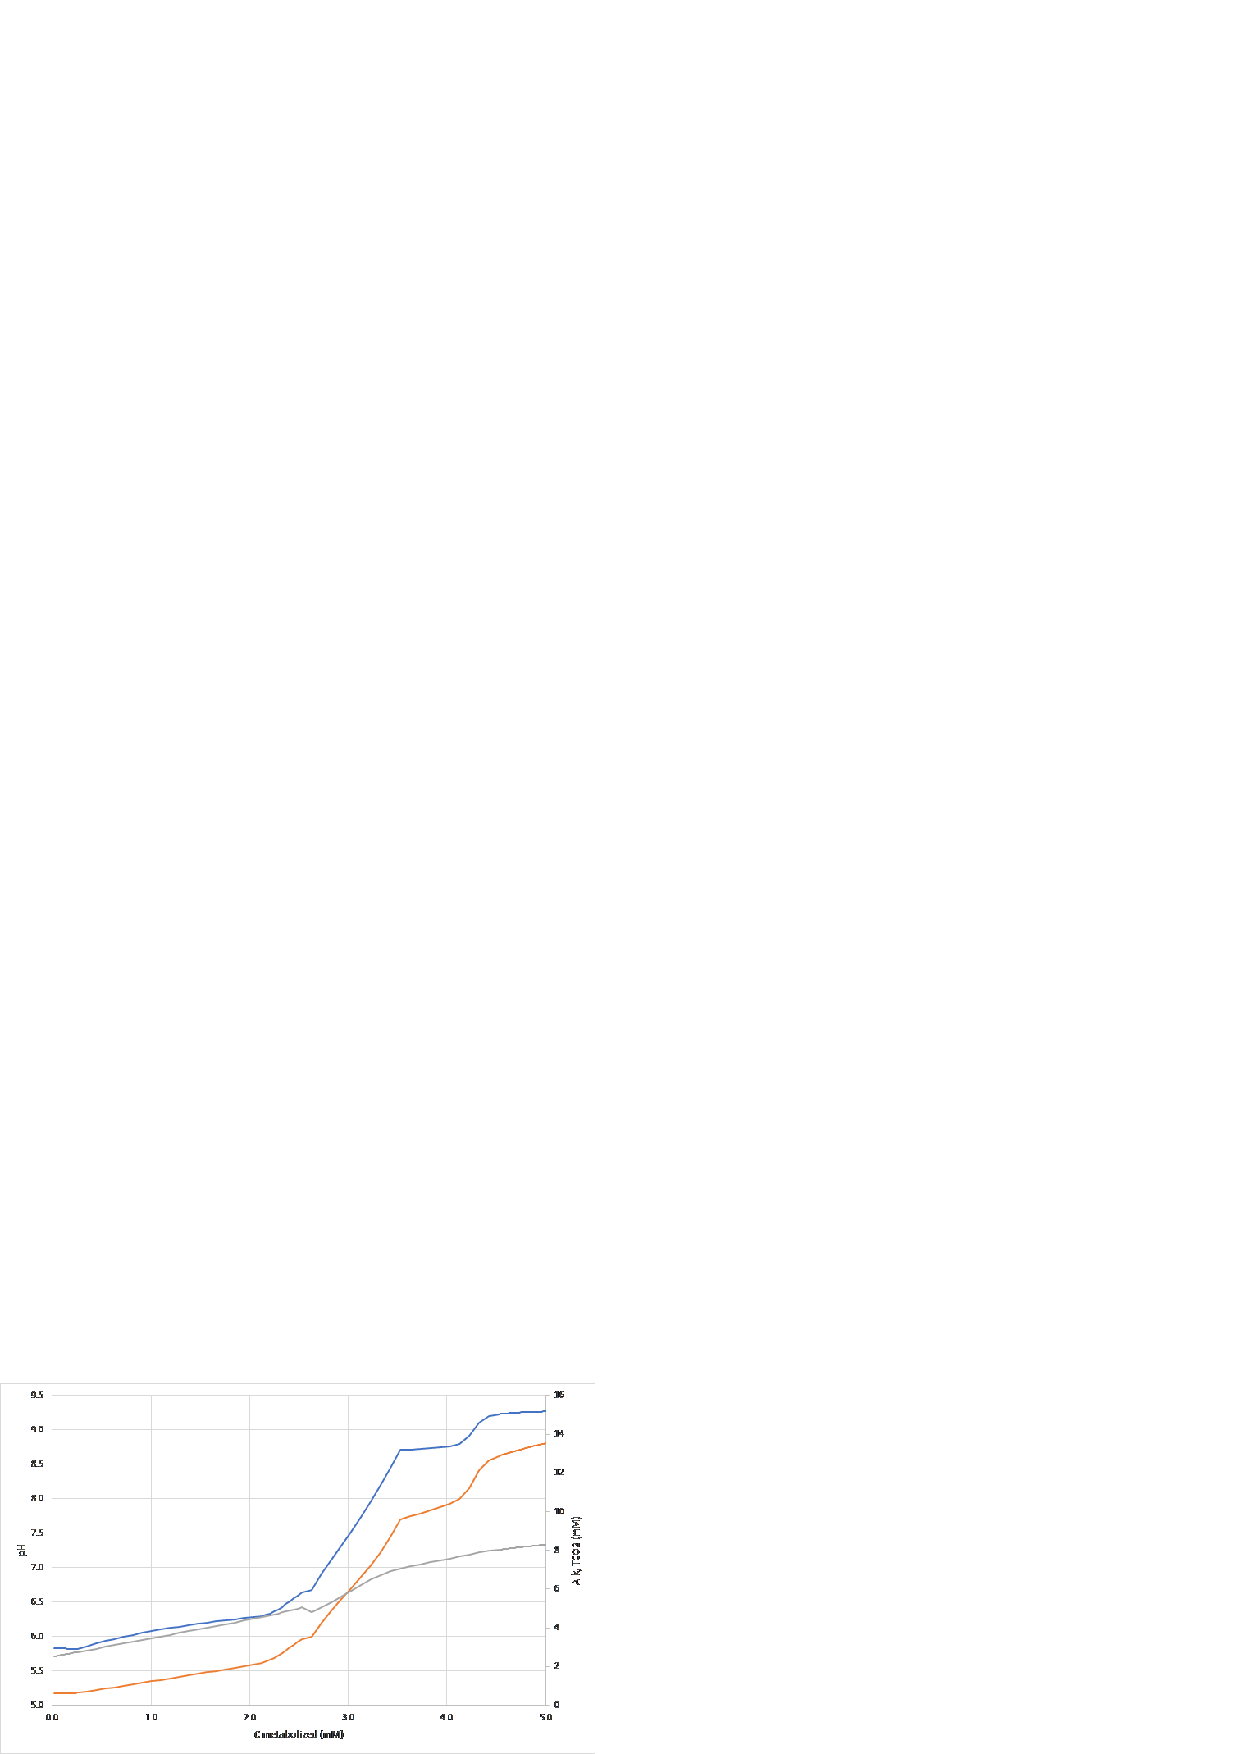
\includegraphics[width=1.0\textwidth, angle = 0]{doug_redox_1}
\caption[]{}
\label{fig:doug_redox_1}
\end{figure}

\begin{figure}[h]
\centering
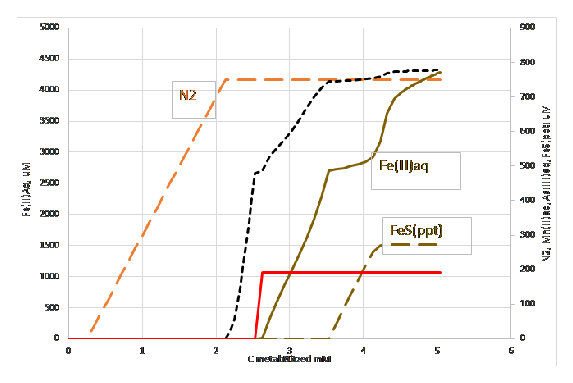
\includegraphics[width=1.0\textwidth, angle = 0]{doug_redox_2}
\caption[]{}
\label{fig:doug_redox_2}
\end{figure}

\begin{figure}[h]
\centering
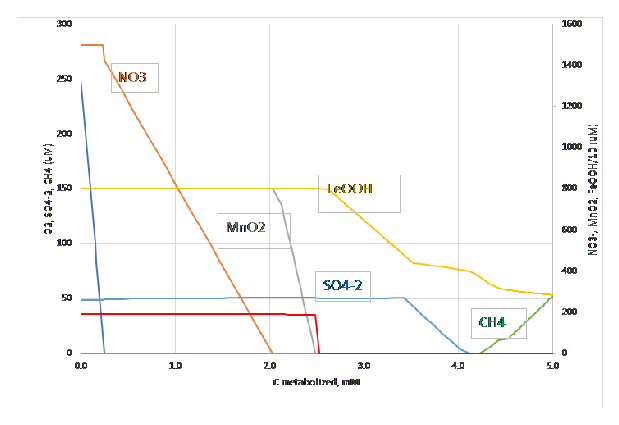
\includegraphics[width=1.0\textwidth, angle = 0]{doug_redox_3}
\caption[]{}
\label{fig:doug_redox_3}
\end{figure}

\begin{figure}[h]
\centering
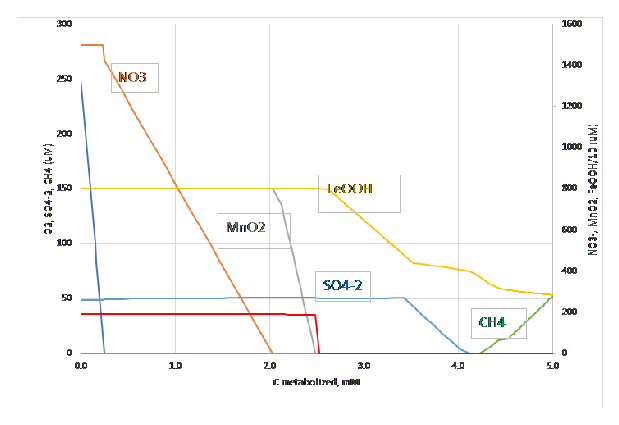
\includegraphics[width=1.0\textwidth, angle = 0]{doug_redox_4}
\caption[]{}
\label{fig:doug_redox_4}
\end{figure}
\section[PHT3D Exercise 7: Artificial recharge and micropollutant fate]{PHT3D Exercise 7: Artificial recharge and micropollutant fate}

\subsection[Background]{Background}
Observed concentrations of reactive solutes in artificially recharged groundwater systems 
can often be highly dynamic and thus puzzling to interpret. For instance, 
concentration variations might be caused by effects, such as temperature variations, 
changes in groundwater flow rates, variations in the injected water quality, or a combination of those. 
One such example where the latter occurs is a study site in Berlin, Germany \citep[]{greskowiak_2006}, 
where aquifers are  recharged by passing wastewater-impacted surface water through 
engineered infiltration ponds, as schematically illustrated in Figure \ref{fig:berlinpond}. 
At this site, the temperature-dependent degradation of sediment-bound 
organic matter (SOM) was an important control for spatiotemporally varying oxygen concentrations. 
However, in addition, highly variable pond infiltration rates caused 
groundwater flow rates to change accordingly and to contribute 
further to the variability of the redox zonation. The model simulations focused 
initially on matching the data collected from in situ temperature loggers, 
and subsequently, the field-observed redox dynamics were replicated. 
In a final step, the degradation behavior of the micropollutant phenazone, 
a pharmaceutical residue, was investigated. 
\par Through the model-based hypothesis testing and data interpretation 
it could be demonstrated that phenazone degraded in this system solely 
under aerobic aquifer conditions that dominated during winter. 
In contrast, phenazone remained persistent under the nitrate-reducing conditions 
that dominated during summer, while oxygen was depleted rapidly (Figure \ref{fig:berlinpond}).
Constraining the groundwater flow and solute transport processes prior 
to evaluating and calibrating the reactive processes associated with oxygen 
consumption allowed for residence time effects to be distinguished from temperature effects.

\par The hypothesized degradation behaviour was based on the results 
of various earlier laboratory experiments that have demonstrated that 
phenazone is biodegradable under oxic conditions \citep{phdzuelke} 
in the presence of the aerobic bacterium $Phenylobakterium$ $immobile$. 
Batch experiments with sterilised and non-sterilised filter material suggest that aerobic microbial
degradation is the most important removal process.
Sorption of phenazone to filter material, sludge, or soil was
found to be negligible. Importantly, it was also found that the degradation
rate of phenazone is temperature-dependent, as its degradation,
like that of organic matter, relies on microbial metabolism.

\par The model simulations in this exercise will employ and discuss the 
model approach that is described in more detail in \cite{greskowiak_2006}. 
The type of redox-sensitive degradation behaviour that is illustrated in 
this exercise was previously also observed for many other micropollutants such as 
pesticides. 

\begin{figure}[tb]
\centering
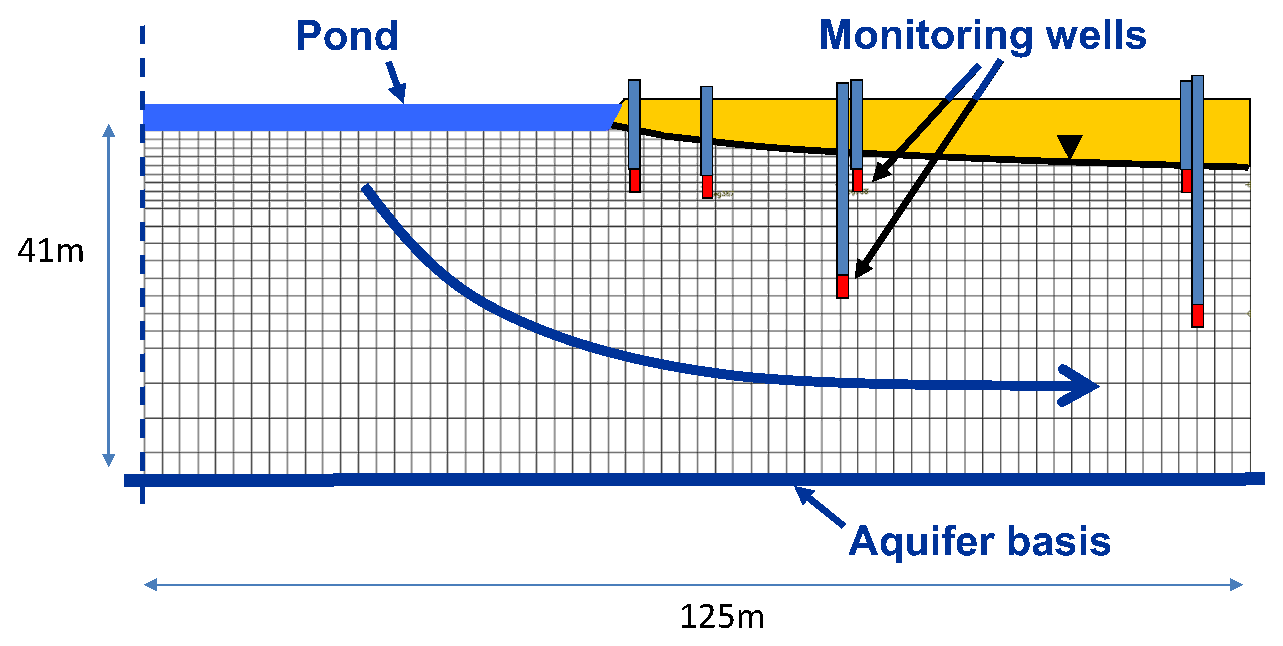
\includegraphics[width=1.0\textwidth]{berlin_transect}
\caption[Schematic figure of the modelled infiltration pond transect]{Schematic figure of the modelled infiltration pond transect} 
\label{fig:berlinpond}
\end{figure}

\subsection[Governing kinetic reactions]{Governing kinetic reactions}
The degradation rate $r_{SOM}$ of the sediment-bound organic matter (SOM) that is present throughout the aquifer
is simulated by a Michaelis-Menten type formulation:

\begin{equation}
r_{SOM} = f_{T} \bigg[ r_{ox} \frac{C_{ox}}{K_{ox} + C_{ox}} + r_{nit} \frac{C_{nit}}{K_{nit} + C_{nit}} 
\frac{K_{ox,inh}}{K_{ox,inh} + C_{ox}}+ r_m \bigg]
\label{eq:som_deg}
\end{equation}

where $f_{T}$ is an empirical function that describes the temperature dependent degradation 
of SOM. 
Thereby $C_{ox}$ and $C_{nitr}$ are the concentrations of dissolved oxygen and nitrate, 
respectively, $r_{ox}$, $r_{nitr}$, $r_{mn}$ are the maximum rate constants under oxic, nitrate reducing 
and manganese reduction conditions, respectively, $K_{ox}$, $K_{nitr}$ are the 
corresponding half-saturation constants, $K_{ox,inh}$ is the inhibition constant 
for nitrate reduction in the presence of oxygen. 
The degradation rate of phenazone is computed from:

\begin{equation}
{r_{phena} = r_{phena,max} {\frac{C_{ox}}{(k_{phena,ox} + C_{ox})}} C_{phena} f_T }
\label{eq:phenazone_deg}
\end{equation}

where $r_{phena,max}$ is the degradation rate constant,
$k_{phena,ox}$ is the half-saturation concentration, 
and $C_{phena}$ represents the concentration of phenazone.

The dependence of the reaction rate 
on the temperature T ($^{\circ}$C) is considered through 
the empirical function, $f_T$, as proposed by \cite{oconnel_1990} 
and \cite{kirschbaum_1995}:

\begin{equation}
{f_{T} = exp({\alpha + \beta T (1 - 0.5 {\frac{T}{T_{opt}}})  )}}
\label{eq:temp_dep}
\end{equation}

where $\alpha$ and $\beta$ are fitting parameters and $T_{opt}$ is the optimal
temperature for the degradation reaction. 
$T$ is the water temperature, 

In the PHREEQC database 
the reaction rate expression for phenazone 
as used in \cite{greskowiak_2006} is formulated such that the reaction 
will only proceed in the presence of dissolved oxygen.

There are two parameters, i.e., ${\color{blue} parm(1)}$
and ${\color{blue} parm(2)}$ that can be modified 
within ORTI under the ${\color{blue} Rates}$ Tab. 
If additional parameters should be edited, 
this can be achieved by editing the 
rate expression below accordingly. 

{\color{red}
\begin{quote}
\#\#\#\#\#\#\#\#\#\#\#\#\#\#\#\#\#\#\#\#\#\#\#\#\#\#\\
Phenazone \\
\#\#\#\#\#\#\#\#\#\#\#\#\#\#\#\#\#\#\#\#\#\#\#\#\#\#\\
\# from Greskowiak et al. 2006 (EST)
-start \\
 7 mTmp   = 1000 * tot("Tmp") \\
10  Cphena = TOT("Phenazone") \\
20  Cox = TOT("O(0)") \\
26  a = -1.5; \\
27  b = 0.18; \\
28  Topt = 35 \\
30  fT = exp(a+b*mTmp*(1-0.5*mTmp/Topt)) \\
34  rph\_max = parm(1) \\
36  Khalf = parm(2) \\
50  rate = fT* rph\_max*(Cox/(Khalf+Cox)) * Cphena \\
70 moles = rate * TIME \\
200 save moles \\
-end \\
\end{quote}}

The present exercise consists of three consecutive, increasingly complex stages: 
\begin{itemize}
\item First we construct a steady-state flow and reactive transport model that simulates 
the fate of phenazone under constant temperature condition
\item Subsequently we modify this model to study the impact of the filed-observed dynamic 
temperature changes and associated with those, the temporal variations in the redox zonation 
\item Finally we also consider the highly variable infiltration rates and s
tudy how this affects the dynamics of the biogeochemical processes.
\end{itemize}


\subsection[Steady flow model]{Steady flow model}
To set up the steady state flow model
\begin{itemize} 
\item Create a new model an set the model up as a 
{\color{blue}confined} 
{\color{blue}Xsection} model within the
{\color{blue}modflow series}.

\item Set the geometry of the model domain with an extension in the x-direction from 0-125 m 
and in z-direction from 0-41 m. 
The grid discretization can be uniform with dx = 6.25m and dz = 4.1m.

\item To assist with the model construction, 
position a map of the cross section (Background\_image.png) to use it as a background image during the model setup. 
To do this use the {\color{blue}Parameters} $\rightarrow$ {\color{blue}Model} $\rightarrow$ {\color{blue}Map} button

\item The total simulation period considered is one year by going to 
{\color{blue}Parameters} $\rightarrow$ {\color{blue}Model} $\rightarrow$ {\color{blue}time} button
and setting the maximum time to 360 days. Set the timestep length to 5 days, which will cause 
the model to force a reaction simulation every 5 days.

\item Position a boundary condition for modflow ({\color{blue}bas.3}) at the right side (east) 
of the cross section from z=0.25m to 33.25m. 

\item Add at the same location a fixed head ({\color{blue}bas.5}) boundary condition at H = 35 m. 
Set the head for the background at 40 m, which will then be used as the starting head of the model.
\end{itemize}

The pond will be considered as a discrete recharge area, while the recharge 
in other areas can be neglected. 
In order to set this recharge area that represents the pond, 

\begin{itemize}
\item Go into the {\color{blue}Addin menu} $\rightarrow$ {\color{blue}modflow modules} 
and select the {\color{blue}RCH} module. To see the module in the interface just click again on modflow. 

\item In this first phase of the exercise we will apply a steady recharge 
rate of 1.4 m/d under {\color{blue}RCH} $\rightarrow$ {\color{blue}rch.2} 
keep the background value at 0 and draw a horizontal line at the model 
top at the location of the pond, i.e., from x=0m to x = 53m, and provide 
a value of 1.4 (m/d). 

\item As the infiltration rate is very high, 
we need to increase the number of internal time steps, 
in order to achieve an adequate numerical solution of the reactive transport problem. 
Click the {\color{blue}Parameter} Button under {\color{blue}Flow} 
and chose {\color{blue}DIS} $\rightarrow$ {\color{blue}dis.8} 
and change the {\color{blue}NSTP} value to 2. 
This results in 2 time steps within each stress period. 

\item Set the hydraulic conductivity to 50 m/d by going to {\color{blue}LPF} $\rightarrow$ {\color{blue}lpf.8} 
and writing 50 in the background box before clicking {\color{blue}ok}. 
This will apply to the whole model. 

\item The vertical hydraulic conductivity 
is set by defining a ratio for Kh/kv. 
To do this go first to {\color{blue}Flow} $\rightarrow$ 
{\color{blue}Parameters} $\rightarrow$ {\color{blue}LPF} $\rightarrow$ {\color{blue}lpf.5} 
and set the value to a ratio kh/kv. 
Then in {\color{blue}Spatial attributes} $\rightarrow$ {\color{blue}modflow} $\rightarrow$ {\color{blue}lpf.9} 
set the value of the ratio of 1 for the whole model (use the background value)

\item Now run MODFLOW.

\end{itemize}

\subsection[Steady flow, chemistry and constant temperature (Stage 1)]
{Steady flow, chemistry and constant temperature (Stage 1)}

To integrate the reactive transport processes into our model 

\begin{itemize}
\item You will first specify the advection scheme that will be used. 
We will select the MOC scheme in 
{\color{blue}Parameters} $\rightarrow$ {\color{blue}Transport} $\rightarrow$ {\color{blue}Parameters} 
$\rightarrow$ {\color{blue}ADV} $\rightarrow$ {\color{blue}adv.1 major data}.
 
\item Subsequently the dispersivity is defined under
{\color{blue}Spatial attributes} $\rightarrow$ {\color{blue}mt3dms} $\rightarrow$ {\color{blue}dsp.2} 
for the longitudinal dispersion, where we will keep the default value of 1 m.

\item Furthermore, we will also leave the ratio of the vertical to 
the longitudinal dispersivity at 0.05. 

\item The porosity (0.35) is set in the 
{\color{blue}Spatial attributes} $\rightarrow$ {\color{blue}mt3dms} $\rightarrow$ 
{\color{blue}btn.11} $\rightarrow$ {\color{blue}porosity}. 

\item Import the pht3d\_datab.dat via the import button under Chemistry. 
You will get a long list of aquoeus components under 
{\color{blue}(Add\_Chemistry} Button $\rightarrow$ {\color{blue}Solutions}. 
However, we will need to activate only a few of those.

\item Check the file {\color{blue}Berlin\_data\_for\_model.xls} sheet stage 1. 
Copy the species values for the {\color{blue}Backgrd} and the {\color{blue}Solu1} column 
from the spreadsheet into the corresponding columns of the ORTi3D interface. 
Check the values, and click those active where at least one value of 
the {\color{blue}Backgrd} and {\color{blue}Solu1} is non-zero. 

\item Note that for numerical reasons 
the species Tmp carrying the Temperature is given in milli $^\circ$C.
This means that, for example, the input value representing a 
temperature of 19 $^\circ$C would be 0.019.

\item Under {\color{blue}Rates}, all {\color{blue}RATES} are imported 
from the {\color{blue}pht3d\_datab.dat} database. 
Select only {\color{blue}Orgc\_sed} and {\color{blue}Phenazone}. 
Also, select {\color{blue}Orgc\_sed} to act as an immobile (IM) species
to reflect the fact that this organic matter is attached to sediments.
\end{itemize}

The {\color{blue}Orgc\_sed} species is here not 
really meant as the concentration of sedimentary organic matter. 
Rather, it is used in here as a reactivity parameter that defines the 
overall reactivity of the organic matter in the aquifer, and linked to the 
consumption of terminal electron acceptors via {\color{blue}RATES} in the database. 
It was assumed that that there is always a sufficient amount of degradable 
organic matter such that it does not 
become rate-limiting. The parameters {\color{blue}parm1} to {\color{blue}parm5} 
correspond to the parameters that are used in the database. 

\begin{table}[b]
\caption{Reaction parameters in the included reaction rate expressions.}
\begin{center}
\begin{tabular}{cccccc}
\toprule
                 & Parm(1) & Parm(2)                  & Parm(3)    & Parm(4)     & Parm(5)        \\
 SOM / Org\_sed  & $r_{ox}$ & $K_{ox}$ = $K_{ox,inh}$  & $r_{nitr}$ &  $K_{nitr}$ & $r_{mn}$ \\
 Phenazone       & $r_{phena,max}$ & $K_{phena,ox}$        &         &         &          \\
 \bottomrule
\end{tabular}
\label{parms_berlin}
\end{center}
\end{table}

All kinetic reaction and temperature parameters are given 
in Table \ref{parm_values_berlin}. 
Note that the constants $T_{opt}$, $\alpha$ and $\beta$ 
were hard-coded in the {\color{blue}pht3d\_database.dat} database 
and don't need to be specified via the ORTi3D user interface.


\begin{table}[b]
\caption{Parameter values for kinetically controlled reactions}
\begin{center}
\begin{tabular}{ccc}
\toprule
  Parameter             &  Value    &    Unit   \\  $\times$ $10^{-3}$ mol/L$_{bulk}$
$r_{ox}$                & 1.32 $\times$ $10^{-5}$  & mol/L/d   \\
$K_{ox}$ = $K_{ox,inh}$ & 1.00 $\times$ $10^{-5}$  & mol/L     \\
$r_{nitr}$              & 3.31 $\times$ $10^{-6}$  & mol/L/d   \\
$K_{nitr}$              & 1.00 $\times$ $10^{-5}$  & mol/L     \\
$r_{mn}$                & 7.70 $\times$ $10^{-8}$  & mol/L/d   \\
$r_{phena,max}$         & 12        & 1/d       \\
$K_{phena,ox}$          & 4.00 $\times$ $10^{-4}$  & mol/L     \\
$T_{opt}$               & 35        & $^{\circ}$C   \\
${\alpha}$            & -1.5      & -             \\
${\beta}$             & 0.18      & 1/$^{\circ}$C \\
 \bottomrule
\end{tabular}
\label{parm_values_berlin}
\end{center}
\end{table}

\begin{itemize}
\item For the rate {\color{blue}Orgc\_sed} the stoichiometry of the reactive constituents 
associated with the reaction has to be entered under 
formula: Enter {\color{blue}Orgc\_sed -1.0 CH2O 1.0 NH3 0.15}.

\item Subsequently enter the formula {\color{blue}Phenazone -1} to be 
associated with the rate of {\color{blue}Phenazone} degradation.

\item Go to {\color{blue}Phases} and click  {\color{blue}Calcite} and provide a background concentration
under {\color{blue}Backg\_Moles} of 1.7 and for {\color{blue}Pyrolusite} 
add a concentration of 3.0 $\times$ $10^{-3}$ under {\color{blue}Backg\_moles} and similarly enter 0 for 
{\color{blue}Rhodochrosite}. 

\item Now we have to assign the aqueous solutions 
that will act as initial and boundary conditions in the model. 
Choose {\color{blue}Pht3d} $\rightarrow$ {\color{blue}PH} $\rightarrow$ {\color{blue}ph.3 Initial concentrations}. 
Make sure that {\color{blue}Backg.} is set to 0, which means that 
solution 0 is used to define the initial water composition.

\item Now choose {\color{blue}ph.5 Recharge}. 
Define a zone that coincides with the infiltration area 
and enter solution number 1 into the right recharge box. 

\item Finally, everything is ready to run PHT3D.
  
\item To visualise the simulation results of, for example, 
temperature, oxygen, nitrate and phenazone at monitoring wells, 
set observations zones {\color{blue}Spatial attributes} 
$\rightarrow$ {\color{blue}observation} $\rightarrow$ {\color{blue}obs.1} 
create lines that span the screened distance of the wells with well names. 
Then, in the panel {\color{blue}results} $\rightarrow$ {\color{blue}observation}, 
select time series graphs and chemistry. 
In the dialog select the wells and then a layer (it can be any layer) 
and click twice on {\color{blue}Apply}. 

\item To better compare the graphs, they may be exported and then 
the txt file can be opened in excel or further processed by python or matlab.

\end{itemize}

\subsection[Seasonal temperature dynamics (Stage 2)]
{Seasonal temperature dynamics (Stage 2)}

\begin{itemize}
\item First, under {\color{blue}Chemistry} $\rightarrow$ 
{\color{blue}Parameters} $\rightarrow$ {\color{blue}PH} 
$\rightarrow$ {\color{blue}ph.6} $\rightarrow$ 
{\color{blue}specific options} and increase the {\color{blue}nb solutions parameter} to {\color{blue}12}.
This will allow to define 12 individual aqueous solutions (default is max 4).  

\item After that re-import the database file {\color{blue}pht3d\_datab.dat}.

\item Under the {\color{blue}Ad\_chemistry} feature, copy the composition from 
solution 1 ({\color{blue}solu1}) to solutions 2 ({\color{blue}solu2}) - solution 12 ({\color{blue}solu12}). 

\item Now you can enter or copy and paste the varying temperatures ({\color{blue}Tmp}) 
for {\color{blue}solu1} to {\color{blue}solu12}. 
The values are provided in the Excel spreadsheet {\color{blue}Stage 2} (indicated in yellow) 
into the ORTi Interface to the species Tmp. 

\item Now choose {\color{blue}ph.5 Recharge}. 
Choose the zone for infiltration area, make it transient, and copy and paste the solution time series 
(time and solution number) given in Sheet {\color{blue}Stage 2} 
(marked in yellow, without the titles) into the right recharge box.
 
\item Run PHT3D and study how the breakthrough curves at the observation wells have changed.
 
\end{itemize}

\subsection[temperature retardation due to heat exchange with the aquifer matrix]{Temperature retardation due to heat exchange with the aquifer matrix}

As now the temperature varies with time in the infiltration water, 
the generated temperature signal in the aquifer will be retarded due to 
heat exchange with the aquifer matrix. The retardation factor depends on the 
thermal characteristics of the porous medium is approximately R = 2.1 in the Berlin aquifer. 
This can be simulated with the {\color{blue}RCT} reaction package, specified 
under MT3DMS (this will automatically also assigned to PHT3D). 
To do so, we have to provide MT3DMS with the apparent density of the medium 
and the Kd to calculate the retardation factor R (R = 1+$rho_{a}$*Kd/porosity). 
With a porosity of 0.35 and a bulk density of 1722 kg/m3, this gives a Kd of 2.2 $\times$ $10^{-4}$. 

\begin{itemize}
\item To set these values you will have to add the {\color{blue}RCT} module to MT3DMS by
(menu {\color{blue}Addin} {\color{blue}mt3dms modules}).

\item then to go to the dialog 
{\color{blue}Parameters} {\color{blue}mt3dms} $\rightarrow$ {\color{blue}Parameters} 
$\rightarrow$ {\color{blue}RCT} $\rightarrow$  {\color{blue}rct.1} 
and set the sorption to linear. 

\item Once this is done go to 
{\color{blue}Spatial attributes} $\rightarrow$ {\color{blue}Mt3dms} $\rightarrow$ 
{\color{blue}Rct} $\rightarrow$  {\color{blue}rct.2a density} 
and set the value at 1722 for the background (i.e., everywhere). 

\item Then go to {\color{blue}Parameters} $\rightarrow$ {\color{blue}Transport} 
and click on {\color{blue}SPC}, 
select {\color{blue}pht3d} in the choice box and write {\color{blue}Tmp} in the species box. 

\item After that, go to {\color{blue}Parameters} $\rightarrow$ {\color{blue}transport} $\rightarrow$ 
{\color{blue}Rct} and you will get a new dialog box with 4 parameters. 

\item Now enter a Kd value of 2.2 $\times$ $10^{-4}$ in the {\color{blue}SP1} column.

\item Re-run PHT3D 

\end{itemize}

Inspect how this changes the time-concentration curves at the observation wells. 
You will notice that now the temperature breakthrough is slightly shifted towards later times, 
as the retardation of the heat transport also affects the redox system and thus ultimately 
also the phenazone breakthrough behaviour.

\subsection[Seasonal temperature and variable infiltration (Stage 3)]
{Seasonal temperature and variable infiltration dynamics (Stage3)}

In this part of the exercise the recharge at the pond (infiltration rate) will changed to a time-varying input
to reflect the highly dynamic changes in infiltration rates that occurred at the field site.
The 1-year long simulation period is therefore split into 12 monthly stress-periods. 
The employed rates are provided in the Excel spreadsheet {\color{blue}Stage 3}.

\begin{itemize} 
\item Select the two columns time and recharge (marked in yellow, without the titles) 
and copy them into ORTi to {\color{blue}RCH} $\rightarrow$ {\color{blue}rch.2}, 
select the recharge zone and click on {\color{blue}value}, which triggers the {\color{blue}zone dialog} to open. 
In this dialog select the {\color{blue}transient} option. A grid will appear in {\color{blue}values}.
Now paste the recharge values that you copied from the spreadsheet into this grid. 

\item Click the {\color{blue}Parameter} Button under {\color{blue}Flow} 
and select {\color{blue}DIS} $\rightarrow$ {\color{blue}dis.8} and change the simulation mode from 
{\color{blue}steady-state} to {\color{blue}transient} simulation.

\item You now need to re-run MODFLOW. You can then check 
how the heads values and gradients are dynamically changing in the model.

\item Finally re-run PHT3D and inspect how the transient recharge affected the breakthrough behaviour.

\end{itemize}



%\include{kinetics/intro}
%\chapter{Modelling kinetically controlled reactions}
\def\shorttitle{Chemical kinetics} % Abbreviated chapter title for right top header

In the preceding chapters we have only considered equilibrium chemistry, i.e. situations where chemical reactions occur instantaneously. For reactive transport problems the simplifying assumption of instantaneous reactions is warranted as long as the reaction time scale is fast compared to the transport time scale, which is known as the local equilibrium assumption \citep[LEA, e.g.,][]{rubin83}.

For many applications, however, the kinetics of chemical reactions have to be considered. Examples include the (slow) dissolution of sillicate minerals, microbially mediated decay of organic pollutants and the oxidation of reduced mineral substances. The versatility of PHREEQC allows for simultaneous modelling of both equilibrium and kinetic processes, which will be the topic of the present chapter. The PHREEQC cases that will be discussed were taken from \cite{prommer_barry_2005}.

\section{MT3DMS Exercise 2: Aerobic biodegradation of hydrocarbons}

\subsection{Objective}

The purpose of this exercise is to gain hands-on experience 
in modeling aerobic biodegradation
of fuel hydrocarbons (BTEX) based on three simple 
approaches, i.e., instantaneous reaction, first-order
kinetics and Monod kinetics. 
The simulation code used in this excise is MT3D99,
however, the same exercise can be carried out 
using RT3D or BIOPLUME III.

\begin{figure}[b]
\centering
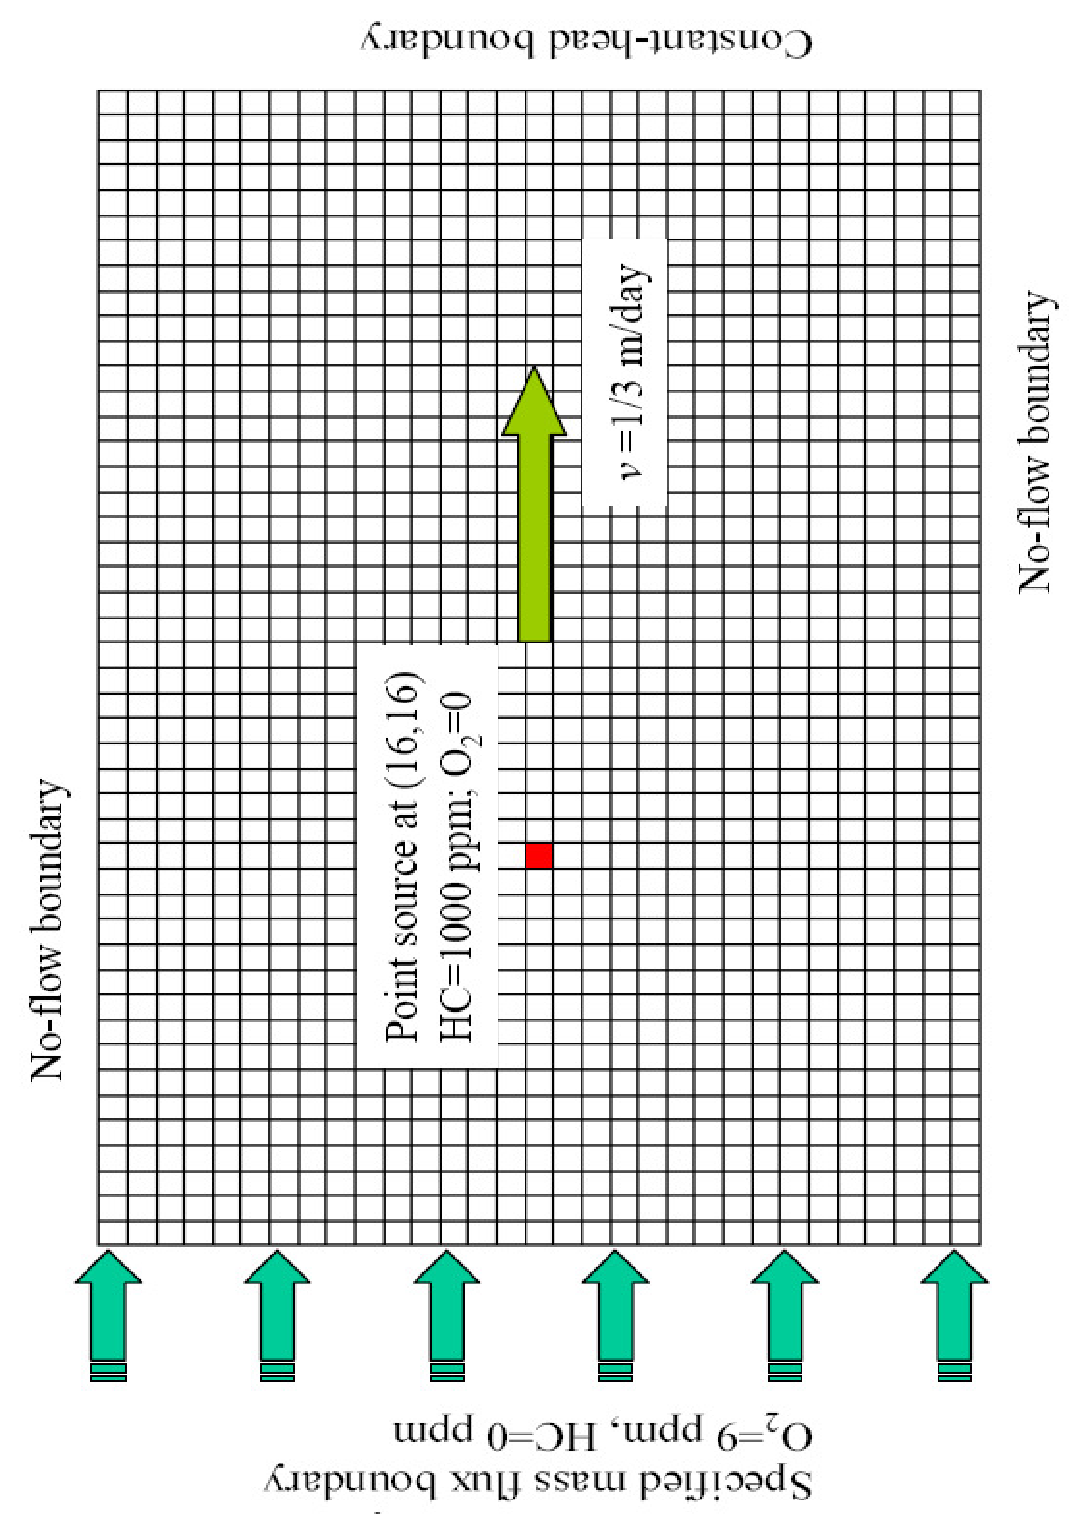
\includegraphics[height=0.9\textwidth,angle=270]{mt3dms_ex2_grid.eps}
\caption[Illustration of the model grid used for MT3DMS Example 2.]{Illustration of the model grid used for MT3DMS Example 2.}
\label{fig:mt3dms_ex2_grid}
\end{figure}

\subsection{Problem Description}

The sample problem considered in this exercise involves 
two-dimensional transport from a
continuous point source in a confined aquifer 
under steady-state flow conditions. The model
grid consists of 46 columns, 31 rows and 1 layer 
and is aligned with the flow direction along the
x axis (see Figure \ref{fig:mt3dms_ex2_grid}). 
The flow model is surrounded 
by constant-head boundaries on the east and
west borders and no-flow boundaries on the north 
and south borders. The head values at the
constant-head boundaries are arbitrarily chosen to 
establish the required hydraulic gradient. 
One injection well is located at column 16 and row 16. 
The injection rate is sufficiently small so that
the flow field remains approximately uniform. 

\begin{table}[hb]
\caption{Flow and solute transport parameters used for MT3DMS Exercise 2.}
\begin{center}
\begin{tabular}{lc} 
\toprule
Parameter                                            &         Value \\
\midrule
Cell width along columns (i-direction) $\Delta x $ $(m)$        &    10 \\
Cell width along rows (j-direction) $\Delta y $ $(m)$           &    10 \\
Layer thickness $\Delta z $ $(m)$                 &    10 \\
Groundwater seepage velocity $(m/day)$              &   1/3 \\
Porosity $\theta$                                         &     0.3 \\
Longitudinal dispersivity $\alpha_L$ $(m)$        &   10 \\
Ratio of transverse to longitudinal dispersivity  &  0.3 \\
Volumetric injection rate $(m^3/day)$               &   1  \\
Simulation time $(days)$                            & 730  \\
\bottomrule
\end{tabular}
\label{aerobic_flow}
\end{center}
\end{table}

\subsection{Flow model}

Set up the flow model using the aquifer dimensions and properties 
listed in Table \ref{aerobic_flow}. Set the hydraulic conductivity K and the
upstream hydraulic heads $h_{upstream}$ to values that will lead to a flow velocity of 1/3 $m/day$.

\begin{equation}
v = 1/3 = K \frac{h_{upstream} -  h_{downstream}} {\theta L}
%\label{eq:retard}
\end{equation}

where $L$ is the distance between the upstream and downstream boundary. To
ascertain confined conditions make sure that
the downstream hydraulic head $h_{downstream}$ is $\ge$ the top of the aquifer.
Do not forget to add the injection well that will be used to inject the contaminant.
Once the model setup is finished:

\begin{itemize}

\item Run MODFLOW

\item Check the flow velocity with the particle tracking software PMPATH.
Select Models $\rightarrow$ PMPATH $\rightarrow$ Options $\rightarrow$ Particle tracking.
Set the Tracking step length to 100 $days$ and use the mouse to define a starting point
near the upstream boundary for a particle tracking simulation. Run the particle tracking simulation.

\end{itemize}

\subsection{Transport model}

Assume that the injected water contains hydrocarbon (species 1) with 
a constant concentration of 1000 $ppm$ ($mg/L$). Further assume that the background concentration of oxygen (species 2) in
the aquifer is 9 $ppm$. The background oxygen concentration is 
modeled by setting the initial
concentration of species 2 to 9 $ppm$ in all model cells and by 
assigning 9 $ppm$ to the species 2
concentration of the inflow from the constant-head boundary. 
Hydrocarbon and oxygen are
assumed to react instantaneously; 
the stoichiometric ratio for the reaction is approximately 3.0.
To start the setup of the reactive transport model

\begin{itemize}

\begin{figure}
\centering
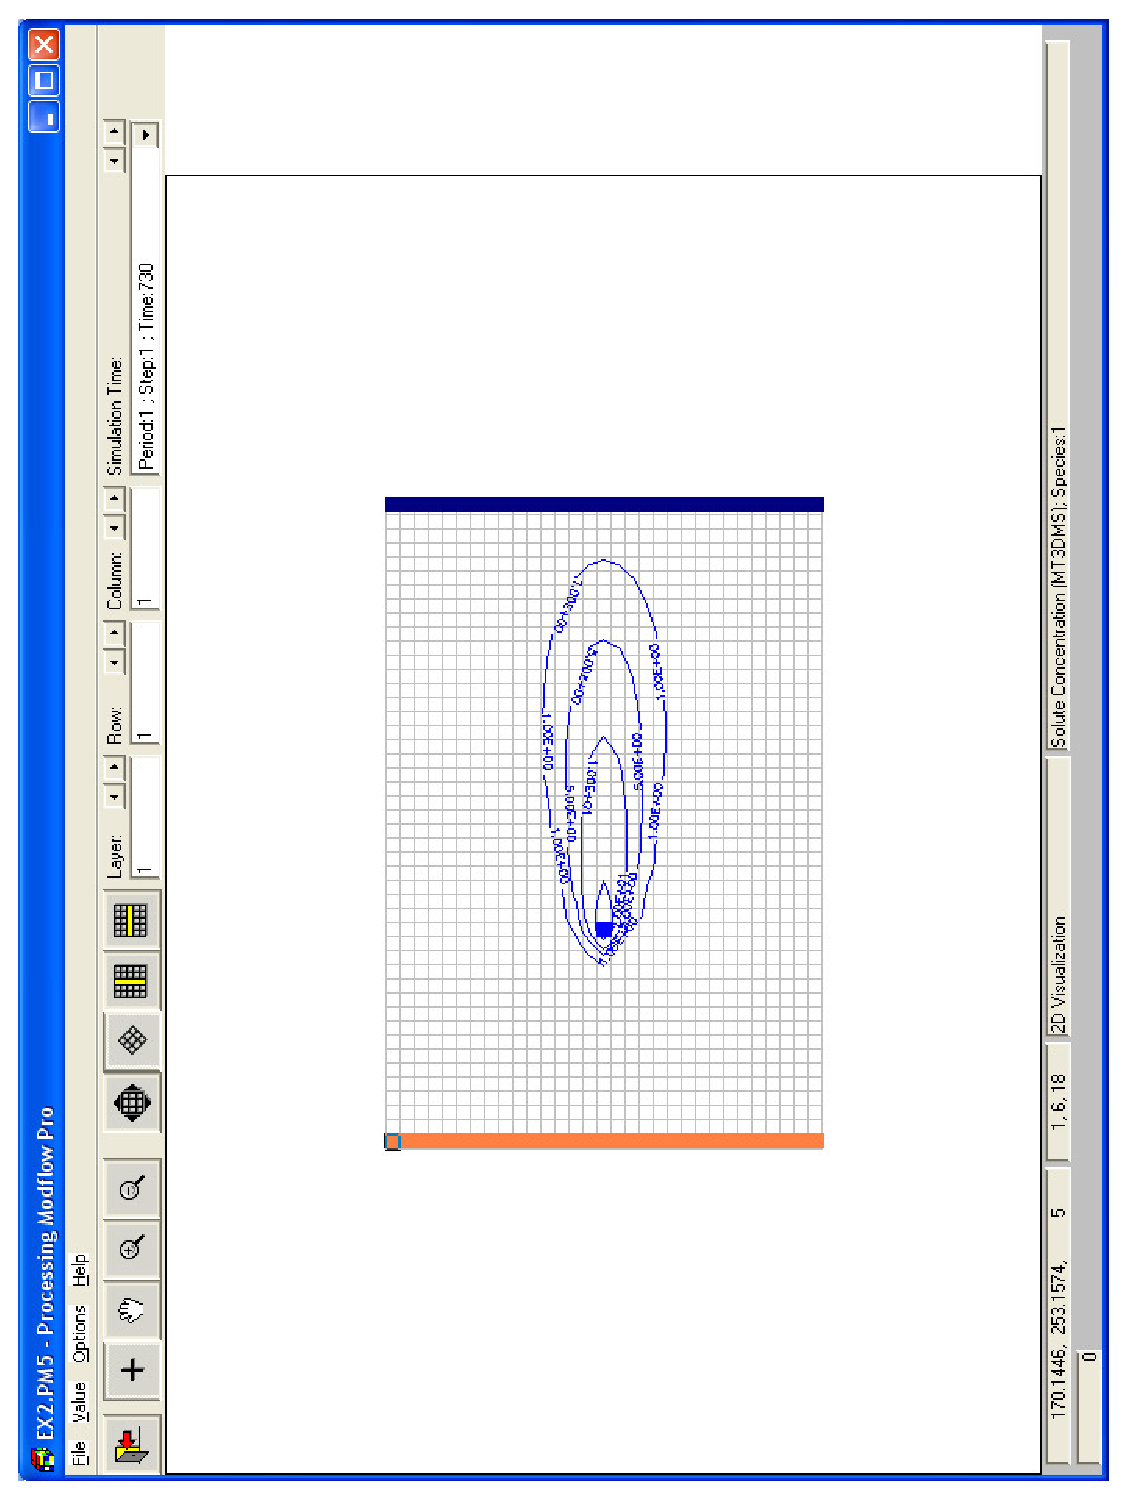
\includegraphics[height=0.89\textwidth,angle=270]{mt3dms_ex2_hc.eps}
\caption[Calculated hydrocarbon concentration distributions at 730 $days$ assuming
instantaneous reactions.]{Calculated hydrocarbon concentration distributions at 730 $days$ assuming
instantaneous reactions.}
\label{fig:mt3dms_ex2_hc}
\end{figure}

\begin{figure}
\centering
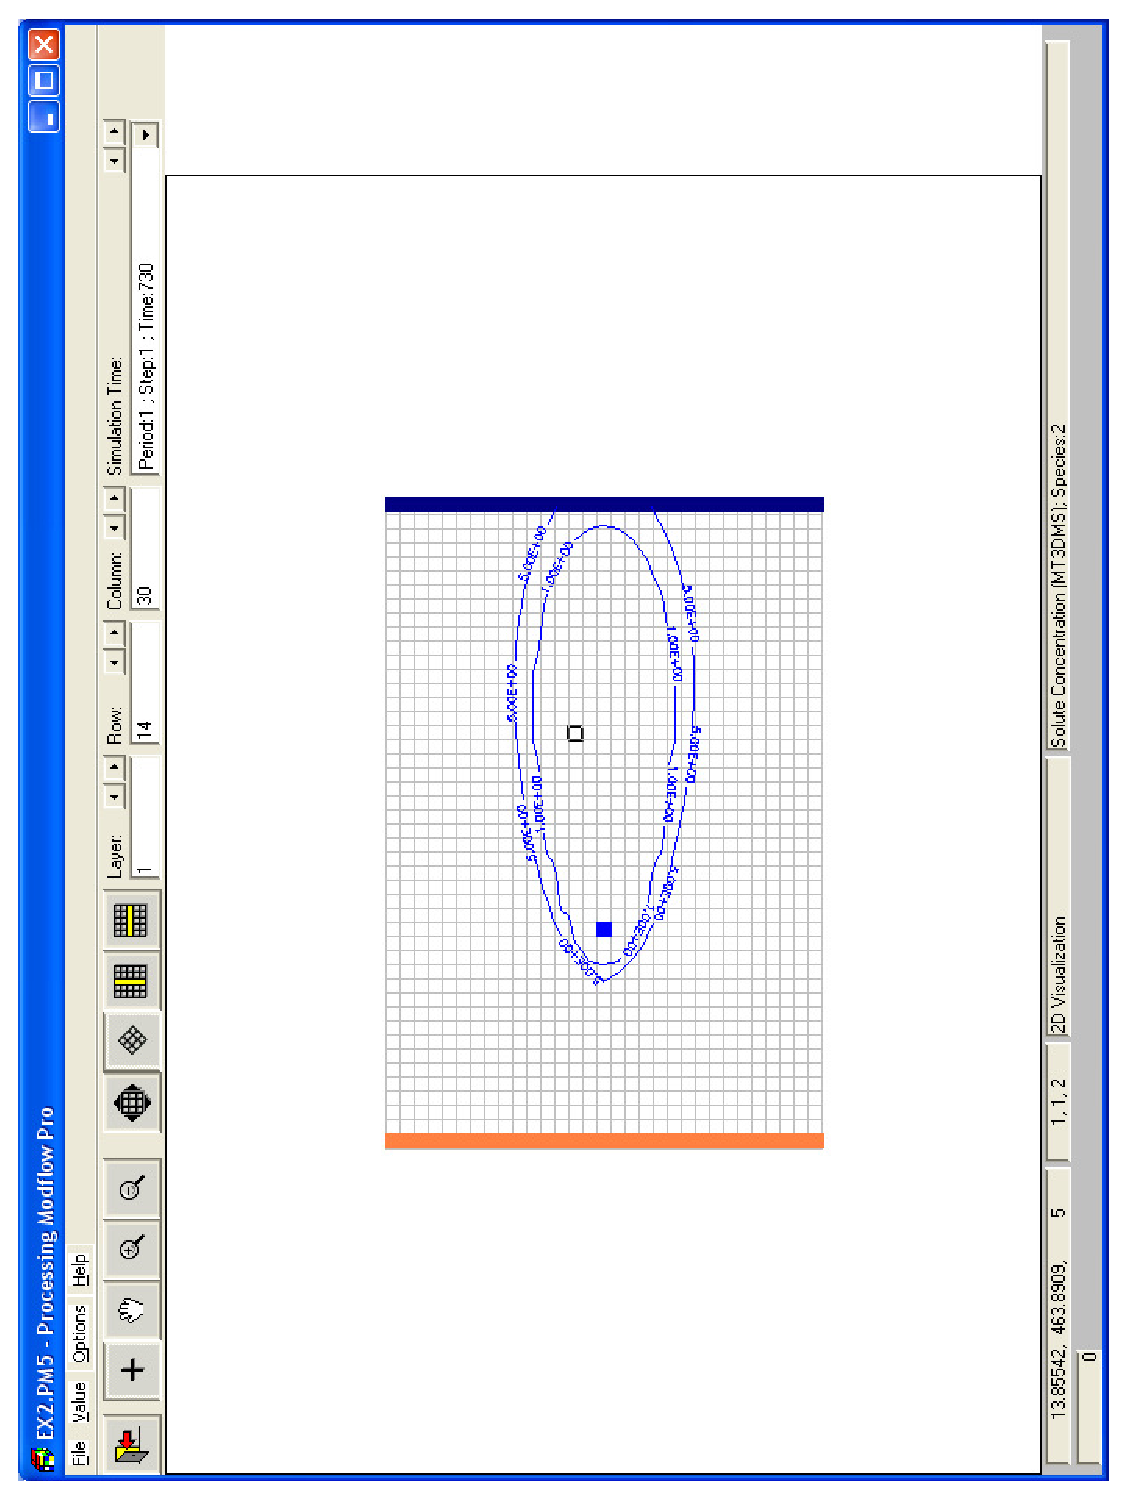
\includegraphics[height=0.89\textwidth,angle=270]{mt3dms_ex2_ox.eps}
\caption[Calculated oxygen concentration distributions at 730 $days$ assuming
instantaneous reactions.]{Calculated oxygen concentration distributions at 730 $days$ assuming
instantaneous reactions.}
\label{fig:mt3dms_ex2_ox}
\end{figure}

\item Select Models $\rightarrow$ MT3DMS $\rightarrow$ Reaction definition and
select Instantaneous reaction among species .
Define Hydrocarbons as species 1 and Oxygen as species 2. Go to 
the Stoichiometry Tab and define the reaction stoichiometry (3.0) for Species pair 
No. 1 - No. 2. Then click OK. Note that the stoichiometric ratio depends on the 
concentration units. If $mol/l$ was used (like it is the case for all PHT3D
concentrations) the value would differ.

\item Set the boundary conditions for concentrations by selecting Select Grid $\rightarrow$ Boundary condition $\rightarrow$ ICBUND (MT3D family). Assign a value of -1
to the cells at the upstream boundary (fixed concentration). 
The default value for ICBUND of 1 (= active cell) will remain
at all other grid cells.

\item Define the initial concentrations by selecting Models $\rightarrow$ 
MT3DMS $\rightarrow$ Initial concentrations. Assign a value of 0 for Hydrocarbons
and a value of 9 $ppm$ for Oxygen.

\item Define the concentration of Hydrocarbons in the 
injected water that simulates the pollution source by selecting Models $\rightarrow$ 
MT3DMS $\rightarrow$ Sink/Source Concentration $\rightarrow$ Well. 
Assign a value of 1000 $ppm$ for Hydrocarbons and a value of 0 $ppm$ for Oxygen
at the grid cell that represents the source zone (column 16, row 16). 

\item Determine which advection package will be used by selecting Models $\rightarrow$ MT3DMS $\rightarrow$ Advection. Select 3rd-order TVD Scheme (ULTIMATE) as the Solution Scheme and click OK.

\item Define the dispersivity to be used by selecting Models $\rightarrow$ MT3DMS $\rightarrow$ Dispersion. In the window that appears, change TRPT to a value of 0.3.
In the editor, use Reset Matrix to change the value for 
the longitudinal dispersivity to 10.0 m. 

\item Run the transport model and visualise the results.

\end{itemize}

The calculated concentrations for hydrocarbon and oxygen at the end of the two-year simulation
period are shown in Figures \ref{fig:mt3dms_ex2_hc} and \ref{fig:mt3dms_ex2_ox}. The maximum concentration of hydrocarbon is approximately 50
ppm at the injection point, as shown in Figure \ref{fig:mt3dms_ex2_hc}. 
The oxygen plume is depleted where the
concentration of hydrocarbon is above zero. 

\subsection{Comparison with First-Order Kinetics}

Next, we will try to simulate the aerobic biodegradation of BTEX using single-species, first-order and Monod kinetics, and compare the simulated BTEX plumes with Figure \ref{fig:mt3dms_ex2_hc}.

First, make a backup copy of the folder that contains the 
instantaneous reaction simulation. 
Then modify the Type of Reaction. Proceeds as follows:

\begin{itemize}

\item Select Models $\rightarrow$ MT3DMS $\rightarrow$ Reaction definition and
select First-order irreversible reaction. Clck OK and leave Editor.

\item  Estimate a first-order rate coefficient and enter the value 
by selecting Models $\rightarrow$ MT3DMS $\rightarrow$ 
Chemical Reactions. Click Edit and start editing the data for
hydrocarbons by selecting Value $\rightarrow$ Reset matrix.
Add your estimated value for the first-order decay rate coefficient.

\item  Run the model and compare the model results (simulated hydrocarbon 
concentrations) with the results from the instantaneous reaction case.
If the two do not agree, the modify the reaction rate coefficient.
Repeat the procedure until you obtain the first-order rate coefficient that leads to a
reasonable match between the simulated plume 
and Figure \ref{fig:mt3dms_ex2_hc} ? What is the final value ?

\end{itemize}

\subsection{Comparison with Monod Kinetics}

Make another copy of the model and use the new copy to explore the effect 
of Monod Kinetics. 

\begin{itemize}

\item Select Models $\rightarrow$ MT3DMS $\rightarrow$ Reaction definition and
select Monod Kinetics. Click OK and leave Editor.

\end{itemize}

Note that Monod kinetics is a nonlinear reaction,
which requires the outer iteration number of the GCG solver 
to be greater than 1. 

\begin{itemize}

\item Select Models $\rightarrow$ MT3DMS $\rightarrow$ Solver $\rightarrow$ 
GCG. Assign a value of 10 for the max. number of outer iterations.

\end{itemize}

Set values for the two Monod kinetics parameters you feel appropriate. Proceed
as follows:

\begin{itemize}

\item Select Models $\rightarrow$ MT3DMS $\rightarrow$ 
Chemical Reactions. Click Edit and start editing the two
parameters.

\item  Run the model and compare the model results (simulated hydrocarbon 
concentrations) with the results from the instantaneous reaction case.

\end{itemize}

If the two do not agree, modify the two parameters. Repeat the
procedure until you obtain the parameter values that result 
in a reasonable match between the
simulated plume and Figure \ref{fig:mt3dms_ex2_hc}. What are the final values?
%\chapter{Modelling kinetically controlled reactions}
\def\shorttitle{Chemical kinetics} % Abbreviated chapter title for right top header

In the preceding chapters we have only considered equilibrium chemistry, i.e. situations where chemical reactions occur instantaneously. For reactive transport problems the simplifying assumption of instantaneous reactions is warranted as long as the reaction time scale is fast compared to the transport time scale, which is known as the local equilibrium assumption \citep[LEA, e.g.,][]{rubin83}.

For many applications, however, the kinetics of chemical reactions have to be considered. Examples include the (slow) dissolution of sillicate minerals, microbially mediated decay of organic pollutants and the oxidation of reduced mineral substances. The versatility of PHREEQC allows for simultaneous modelling of both equilibrium and kinetic processes, which will be the topic of the present chapter. The PHREEQC cases that will be discussed were taken from \cite{prommer_barry_2005}.

%\section{Modelling bioremediation processes}
In order to be able to design active bioremediation systems and to understand passive bioremediation (natural attenuation), mechanistic descriptions that quantify microbial activity are needed. Since both the rate of microbial growth and the rate of contaminant utilization are highly dependent on the amount of biomass available to catalyze the reactions, such models must have the capability to predict both transient and spatial variations in biomass. To model the production of biomass and the related consumption and production of other chemicals, the key steps are (1) to formulate the rate expressions for the reaction kinetics and (2) to determine the stoichiometry of the biodegradation reactions and, in order to describe the temporal variations.

In the macroscopic mathematical descriptions of microbial growth dynamics aimed at governing laboratory or field scale processes, many of the complex interdependencies that are known at the microscopic scale are commonly neglected and described by empirical formulations based on the classical works of \cite{michmen} and \cite{monod}. The expression describing a specific bacterial growth rate, $v_{sp}$, observed in many batch experiments is:
\begin{equation}
v_{sp} = v_{max} \frac{C_{org}}{K_{org} + C_{org}}
\label{eq:v_sp}
\end{equation}
where $C_{org}$ is the concentration of the organic substrate, $v_{max}$ is an assymptotic maximum specific uptake rate and $K_{org}$ is the half-saturation constant, which is the substrate concentration at which the actual uptake rate equals $v_{max} / 2$. Based on equation \ref{eq:v_sp}, the total uptake rate $v_m$ considers the dependency of the change of microbial mass on the actual microbial concentration $X$ itself:
\begin{equation}
v_{m} = v_{max} \frac{C_{org}}{K_{org} + C_{org}} X
\label{eq:v_m}
\end{equation}

An additional (potential) growth limitation by electron acceptor availability might be incorporated into \ref{eq:v_m}, leading to:
\begin{equation}
v_{m} = v_{max} \frac{C_{org}}{K_{org} + C_{org}} \frac{C_{ea}}{K_{ea} + C_{ea}} X
\label{eq:v_m_ea}
\end{equation}
where $C_{ea}$ is the electron acceptor concentration and $K_{ea}$ is the appropriate half-saturation constant.

The complete mass balance equation for the microbial mass, $X$, describing the change of microbial concentration as a function of time, includes both a microbial growth and decay term:
\begin{equation}
\frac{\partial X}{\partial t} = \frac{\partial X_{growth}}{\partial t} + \frac{\partial X_{decay}}{\partial t}
\end{equation}
with
\begin{equation}
\frac{\partial X_{growth}}{\partial t} = Y_x v_{max} \frac{C_{org}}{K_{org} + C_{org}} \frac{C_{ea}}{K_{ea} + C_{ea}} X = Y_x v_m
\label{eq:X_growth}
\end{equation}
in which $Y_x$ is a stoichiometric factor and
\begin{equation}
\frac{\partial X_{decay}}{\partial t} = -v_{dec} X
\label{eq:X_decay}
\end{equation}
where $v_{dec}$ is a decay rate constant.

During growth ($v_m > 0$), both organic substrate and electron acceptors are consumed at rates that are proportional to $v_m$, which will be illustrated in the following example of toluene degradation under sulfate-reducing conditions.

\subsection{PHREEQC Example: Kinetic toluene degradation}
The stoichiometry of the reactions that describe the microbial degradation of organic compounds depends on the efficiency of the microorganisms to divert electrons (gained in the oxidation step) to either biomass generation or towards electron acceptors. Assuming that 10\% of the carbon is incorporated into biomass, the oxidation of toluene under sulfate-reducing conditions can be described by the following overall reaction:

\begin{eqnarray}
C_7H_8 + 0.14NH_4^+ + 4.15 SO_4^{-2} + 2.58H_2O + 1.86H^+ \rightarrow  \nonumber \\
 \ \  \  \  \  6.30HCO_3^- + 0.14 C_5H_7O_2N + 4.15 H_2S
\label{eq:tol_sulf}
\end{eqnarray}

Equation \ref{eq:tol_sulf} shows that the complete mineralization of 1 mol of toluene consumes 4.15 mol of sulfate (during growth) and yields 0.14 mol of sulfate-reducing bacteria (represented by the genralized chemical formula for biomass: $C_5H_7O_2N$). Therefore:

\begin{equation}
\frac{\partial X_{growth}}{\partial t} = 0.14 v_m
\end{equation}

and

\begin{equation}
\frac{\partial C_{sulf}}{\partial t} = -4.15 v_m
\end{equation}

These equations can be implemented in PHREEQC to compute the temporal development of toluene, sulfate and the microbial mass in a batch experiment. Tables \ref{tab:tol_sulf_conc} and \ref{tab:tol_sulf_const} list the initial conditions and rate constants for the simulation.

\begin{table}[hb]
\topcaption{Initial concentration for simulation of a batch experiment of toluene degradation under sulfate-reducing conditions.}

\centering
\footnotesize
\begin{tabular*}{0.5\textwidth}{@{\extracolsep{\fill}}ll}
\toprule
Component & Concentration \\
          & mol/l \\
\midrule
Toluene  & $1.0 \cdot 10^{-4}$ \\
N & $1.0 \cdot 10^{-4}$ \\
S(6) &  $4.5 \cdot 10^{-4}$ \\
Sulfred$^1$ &  $1.0 \cdot 10^{-8}$ \\

\bottomrule
\raggedright $^1$ Sulfred: sulfate reducing bacteria
\end{tabular*}
\label{tab:tol_sulf_conc}
\end{table}

\begin{table}[b]
\topcaption{Rate constants for simulation of a batch experiment of toluene degradation under sulfate-reducing conditions.}

\centering
\footnotesize
\begin{tabular*}{0.5\textwidth}{@{\extracolsep{\fill}}ll}
\toprule
Component & Constant \\
\midrule
$K_{sulf}$ (mol/l)    & $1.0 \cdot 10^{-5}$ \\
$K_{toluene}$ (mol/l) & $1.0 \cdot 10^{-5}$ \\
$v_{max}$ (1/day)       & 5.0                 \\
$v_{dec}$ (1/day)       & 0.1                 \\

\bottomrule
\end{tabular*}
\label{tab:tol_sulf_const}
\end{table}

The input file {\color{red}toluene\_degradation.phrq} is available and can be opened
in PHREEQC for Windows. Two new aqueous species are defined in the input file that represent toluene (species name: Toluene) and $X$ (species name: Sulfred, since X is already reserved for exchange species). 

The rate expressions for toluene degradation and biomass decay are defined under the keyword \textbf{RATES}. They are programmed in BASIC, which can be interpreted by PHREEQC so that any type of user-defined rate expression can be modelled.

\begin{quote}
{\color{red}
	RATES \\
	Toluene\_sulf \\
    -start \\
    1   k\_Tolu    = 1e-05 \\
    2   k\_Sulf    = 1e-05 \\
    4   v\_up\_max  = 5.0/86400 \\
    10  mTolu     = TOT("Toluene") \\
    22  mSulf     = TOT("S(6)") \\
    30  mSulfred  = TOT("Sulfred") \\
    32  IF (mTolu $<$ 1e-08) THEN GOTO 200 \\
    34  IF (mSulf $<$ 1e-09) THEN GOTO 200 \\
    40  mon\_Tolu  = mTolu / (k\_Tolu + mTolu) \\
    50  mon\_Sulf  = mSulf / (k\_Sulf + mSulf) \\
    80  growth    = v\_up\_max*mon\_Tolu*mon\_Sulf*mSulfred \\
    100 rate      = growth \\
    110 moles     = rate * TIME \\
    200 SAVE moles \\
    -end \\ 
}
 \\
{\color{red}
Sulfred \\
    -start \\
   10 v\_decay   = 0.1/86400 \\
   15 c\_min     = 1e-08 \\
   20 mSulfred  = TOT("Sulfred") \\
   30 IF (mSulfred - c\_min  $>$ 0) THEN inhibit\_fac\_decay = (mSulfred - c\_init)/mSulfred \\
   35 IF (mSulfred - c\_min  = 0) THEN inhibit\_fac\_decay = 0 \\
   40 IF (mSulfred - c\_min  $<$ 0) THEN inhibit\_fac\_decay = 0 \\
  190 rate      = v\_decay*mSulfred*inhibit\_fac\_decay \\
  200 moles     = rate * TIME \\
  220 SAVE moles \\
 -end \\
}
\end{quote}

Try to understand the syntax here. In lines 1, 2 and 4 of the toluene degradation rate block, the constants from table \ref{tab:tol_sulf_const} are specified. Then, the total concentrations of the aqueous components Toluene, S(6) (sulfate) and sulfate reducing bacteria are read from PHREEQC's internal memory (lines 10, 22 and 30). Then in lines 32 and 34, a check is carried out to make sure that the concentrations of toluene and sulfate are sufficiently high. Otherwise, the rest of the code is skipped, which means that the rate becomes zero. Lines 40, 50 and 80 implement the actual rate expression according to equation \ref{eq:X_growth}. The number of moles that react are calculated by multiplying the rate times the duration of the time step (the TIME parameter) in line 110 and passed back to PHREEQC in line 200 with the SAVE statement.

The rate expression for the decay of the sulfate reducing bacteria is constructed in a similar way under the identifier Sulfred. Note that an extension of equation \ref{eq:X_decay} is used in line 30 to limit the decay rate by multiplying with $(X - X_{init})/X$, where $X_{init}$ is the initial concentration of sulfate reducing bacteria.

The \textbf{KINETICS} keyword actually incorporated the rate expressions into the PHREEQC simulation. The names of the rate expressions are listed (Toluene\_sulf and Sulfred) and the identifier -steps takes care of the temporal discretization. The -formula identifiers control the stoichiometric proportions of aqueous species which are released or consumed per mole kinetic reactant. In this example, for case a, 0.14 moles of sulfate reducing bacteria are produced for each mole of toluene reacted, which removes 0.14 moles of $\text{C}_5\text{H}_7\text{O}_2\text{N}$ from the solution. A negative stoichiometric coefficient indicates that a species is removed from the solution for each mole of kinetic reactant formed, which is why the stoichiometric coefficient for toluene is -1.

The keyword \textbf{USER\_GRAPH} control the graphical output of this simulation. If you go to the Chart tab in PHREEQC for Windows and start the calculations you can even see the chart being filled with data points during the calculation. The BASIC statements GRAPH\_X, GRAPH\_Y and GRAPH\_SY allocate numbers to the x-, y- and secondary y-axes respectively. The identifiers are basically self-explanatory.

Notice that two cases are considered in this example: case a and case b. Case b differs from case a in that the effects of the different valence state of bacteria (compared to the end-product $\co$) and the related geochemical changes are not considered. All sulfate is consumed during bacterial growth but none during bacterial decay.

Run the model for case a first and look a the chart. Notable is the lag-period of several days before the degradation affects the aqueous concentrations of toluene and sulfate. Its length depends largely on the initial bacterial concentration and on $v_{max}$, the maximum uptake rate (values given in tables \ref{tab:tol_sulf_const}). The removal of the initial toluene mass (0.1 mmol) is reached after 14 days, at a time when approximately 0.415 mmol of sulfate are depleted. The microbial (net) growth then stops immediately ($v_m = 0$) and the microbial mass is subsequently changing at the rate given by equation \ref{eq:X_decay}, thereby consuming the remaining 0.35 mmol of sulfate.

You can switch to case b by switching the \#-signs in front of the -formula identifier under \textbf{KINETICS}. Now all sulfate is consumed during bacterial growth but none during bacterial decay. Run the simulation and observe the resulting chart.

\subsection{PHREEQC Exercise 5: Kinetic BTEX degradation}
Of course, the formulations for microbial growth above apply only to the uptake of a single substrate, whereas contamination often involves numerous (organic) compounds. The (possibly simultaneous) uptake of these substrates can be incorporated into the modeling approach described above. The model of \cite{kincel89} states that the growth of the degrading microbial community is simply the sum of the growth rates arising from degradation of individual organic contaminants:
\begin{equation}
\frac{\partial X}{\partial t} = \left[ \left(\sum_{n=1}^{n_{org}} \frac{\partial X_{n}}{\partial t}\right) - v_{dec} \right] X
\end{equation}
where, in analogy to equation \ref{eq:X_growth}, each of the growth terms $\frac{\partial X_{n}}{\partial t}$ can be derived from:
\begin{equation}
\frac{\partial X_{n}}{\partial t} = Y_x v_{max}^n \frac{C_{org,n}}{K_{org,n} + C_{org,n}} \frac{C_{ea}}{K_{ea} + C_{ea}}
\label{eq:X_growthn}
\end{equation}

The uptake rates $v_{max}^n$ can differ between different substrates. In this way, it is possible to model varying degradation rates of different electron donors. This can be necessary when, for example, benzene degrades more slowly in a BTEX (benzene, toluene, ethylbenzene, xylenes) plume than the other compounds. In this exercise, you will model a case of a simultaneous uptake of BTEX constituents by one microbial group. Different initial amounts of organic compounds are present (Table \ref{tab:btex_conc}) and the initial sulfate mass is increased compared to the first example.

\begin{table}[hb]
\topcaption{Initial concentration for simulation of a batch experiment of BTEX degradation.}

\centering
\footnotesize
\begin{tabular*}{0.5\textwidth}{@{\extracolsep{\fill}}ll}
\toprule
Component & Concentration \\
          & mol/l \\
\midrule
Benzene  & $4.0 \cdot 10^{-4}$ \\
Toluene  & $3.0 \cdot 10^{-4}$ \\
Ethylbenzene  & $1.0 \cdot 10^{-4}$ \\
Xylene  & $2.5 \cdot 10^{-4}$ \\
N & $1.0 \cdot 10^{-4}$ \\
S(6) &  $5.0 \cdot 10^{-4}$ \\
Sulfred$^1$ &  $1.0 \cdot 10^{-8}$ \\

\bottomrule
\raggedright $^1$ Sulfred: sulfate reducing bacteria
\end{tabular*}
\label{tab:btex_conc}
\end{table}

\begin{table}[hb]
\topcaption{Rate constants for simulation of a batch experiment of BTEX degradation.}

\centering
\footnotesize
\begin{tabular*}{0.5\textwidth}{@{\extracolsep{\fill}}ll}
\toprule
Component & Constant \\
\midrule
$K_{sulf}$ (mol/l)    & $1.0 \cdot 10^{-5}$ \\
$K_{benzene}$ (mol/l) & $1.0 \cdot 10^{-5}$ \\
$K_{toluene}$ (mol/l) & $1.0 \cdot 10^{-5}$ \\
$K_{ethylbenzene}$ (mol/l) & $1.0 \cdot 10^{-5}$ \\
$K_{xylene}$ (mol/l) & $1.0 \cdot 10^{-5}$ \\
$v_{max,sulf,benzene}$ (1/day)       & 0.1   \\
$v_{max,sulf,toluene}$ (1/day)       & 5.0   \\
$v_{max,sulf,ethylbenzene}$ (1/day)  & 0.5   \\
$v_{max,sulf,xylene}$ (1/day)  			 & 1.0   \\
$v_{dec}$ (1/d)       & 0.1                 \\

\bottomrule
\end{tabular*}
\label{tab:btex_const}
\end{table}

The corresponding reaction equations are, for benzene:

\begin{eqnarray}
C_6H_6 + 0.12NH_4^+ + 3.45 SO_4^{-2} + 2.64H_2O + 1.38H^+ \rightarrow \nonumber \\
 \ \  \  \  \ 5.4HCO_3^- + 0.12 C_5H_7O_2N + 3.45 H_2S
\end{eqnarray}
and for ethylbenzene and xylene(s):
\begin{eqnarray}
C_8H_10 + 0.16NH_4^+ + 4.85 SO_4^{-2} + 2.52H_2O + 2.34H^+ \rightarrow \nonumber \\
 \ \  \  \  \ 7.2HCO_3^- + 0.16 C_5H_7O_2N + 4.85 H_2S
\end{eqnarray}

The PHREEQC input file for this exercise is already prepared and available as {\color{red} btex\_degradation.phrq}. However, you still need to insert some numbers to make it work. Fill in the parameters from table \ref{tab:btex_const} at the appropriate locations (these are marked with \#-signs).

Run the file and inspect the change of BTEX with time on the Chart tab. Write down the order in which the 4 different compounds degrade:

\begin{enumerate}

\item 

\item

\item

\item

\end{enumerate}

The \textbf{USER\_GRAPH} keyword block is set up in such a way that the concentrations of the individual BTEX compounds are plotted in the chart. Modify it to have the concentrations of the biomass and nitrogen displayed instead.

\begin{itemize}

\item Explain the temporal concentration patterns of the biomass and nitrogen.

\end{itemize}
%\include{kinetics/prommer_davis_barry_ipht3d}
%\include{arsenic/arsenic_vp_orti}
%\include{kinetics/prommer_stuyfzand_ipht3d_sustech}
%\section[PHT3D Exercise 7: Degradation of chlorinated ethenes and isotopes]{PHT3D Exercise 7: Degradation of chlorinated ethenes and isotopes}

\subsection[Modelling Scenario]{Modelling Scenario}

In this exercise we investigate the sequential degradation of chlorinated ethenes and the use of 
stable isotopes to provide forensic evidence for the origin of elevated vinyl chloride concentrations in a pumping well.   

The principle modelling scenario consists of an aquifer that is contaminated by two different contaminant spillages, both positioned below sites of former metal processing companies (Company E and Company W). The modelling scenario is set up for a vertical cross section. The two different contamination sources consist of NAPL pools that are located on top of clay lenses. One of the NAPL sources is assumed to consist of PCE (tetrachlorethylene), while the other is assumed to consist of a mixture of TCE (trichlorethylene) and toluene. Groundwater is entering the model domain through the Eastern (fixed hydraulic head = 13.7 m.a.s.l) and Western boundary (fixed hydraulic head = 14.5 m.a.s.l). Under natural conditions the groundwater discharges to the river (prescribed hydraulic head = 10.8 m.a.s.l). However, there is also an active pumping well located between the PCE source and the river. The majority of the water that enters the model domain through the fixed head boundary discharges to the well during active pumping. However, some groundwater infiltrates to the river. On the other hand, some river water is also drawn towards the pumping well. The model setup is shown in Figure \ref{fig:ex6_setup}

\begin{figure}[here]
\centering
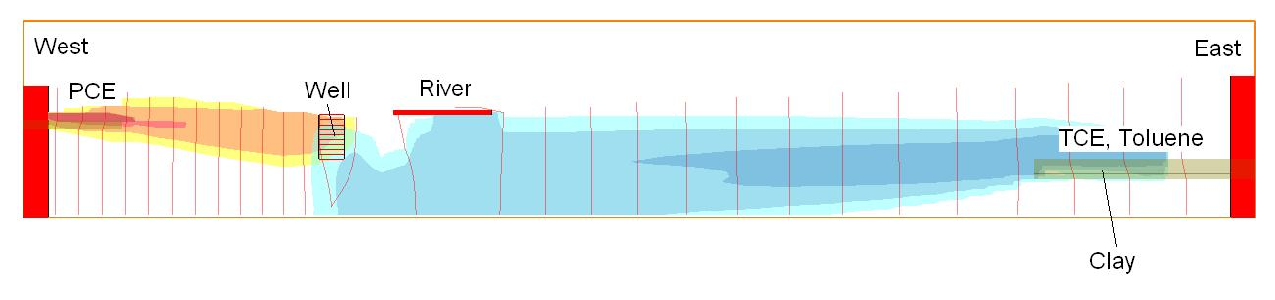
\includegraphics[width=\textwidth]{ex6_setup}
\caption[PHT3D Exercise 7: Model setup]{PHT3D Exercise 7: Model Setup}
\label{fig:ex6_setup}
\end{figure}

\subsection[NAPL source zones]{NAPL source zones}

The contamination sources are modelled by defining two discrete NAPL contaminated zones.
On the Western side of the river a PCE source is defined by allocating an initial 
concentration of 1 mol/l of Pcenapl to a discrete source zone situated on top of the clay lense.
Similarly, the Eastern source is defined by allocating 1 mol/l of Tcenapl and 1 mol/l of Tolunapl 
to a discrete zone.

The rate expression that controls the kinetically controlled release of PCE is \\

{\color{red}
\begin{quote}   
\#----------------------------------------------- \\
Pcenapl		\\
\#----------------------------------------------- \\
  -start \\
   10  mPcenapl = tot("Pcenapl") \\
   15  if (mPcenapl $<=$ 1e-10) then goto 200 \\
   20  solub\_Pce = 1.28 / 131.39 \# aqueous solubility of PCE \\
   22  frac\_of\_solub = parm(2) \# Fraction of single species solubility\\
   25  mPce = tot("Pce\_l") + tot("Pce\_h") \\
   50  msolub\_Pce =  frac\_of\_solub * solub\_Pce \\
   60  rate = parm(1) * (msolub\_Pce - mPce) \\
   65  if (mPce $>$ msolub\_Pce) then rate = 0 \\
   70  moles = rate * time \\
   80  if (moles $>$ m) then moles = m \\
   200 save moles \\
  -end \\
 \end{quote}
 }
 
 In the reaction database similar rate expressions are defined for TCE and toluene.
 
\subsection[Formation of dissolved plumes]{Formation of dissolved plumes}

When groundwater passes through these zones, dissolution (mass transfer to the aqueous phase) will
occur, therefore creating a PCE plume on the Western side of the river. On the Eastern side of the 
river the NAPL source creates a TCE as well as a toluene plume. 

During the simulation period of 10 years these plumes grow initially but eventually become stable, given that we assume steady-state flow and constant source release conditions. This means that chemical concentrations at a particular location are not changing any further after a specific simulation time. 

\subsection[Degradation reactions]{Degradation reactions}

Besides the plumes of the primary contaminants there are also plumes of the transformation products developing. 
These result from the degradation reactions that may proceed in suitable hydrochemical and microbial conditions.

Under the oxic conditions found in this river valley aquifer the toluene plume released from the NAPL source
undergoes aerobic degradation, thereby consuming oxygen. On the Eastern side of the model domain this 
creates locally anaerobic conditions between the NAPL source and the groundwater discharge locations. 

\begin{itemize}

\item Visualise the contours of the toluene plume (Tolu\_l) after 10 years (3650 days) simulation time.

\item Visualise the oxygen concentration contours after 10 years (3650 days) simulation time.
 
\end{itemize}

Where these anaerobic conditions prevail reductive dechlorination of TCE may take place.
The transformation follows typically a sequential degradation pathway 
(TCE $\rightarrow$ DCE $\rightarrow$ VC $\rightarrow$ Ethene).  
In our model this reaction pathway is incorporated as a sequence of simple first oder reactions. 
The corresponding reaction rate expression is, for exmaple for TCE:  \\

{\color{red}
\begin{quote}   
\#----------------------------------------------- \\
Tce\_l		\\
\#----------------------------------------------- \\
  -start \\
2  if (tot("O(0)")) $>$ 1e-7 then goto 60 \\
5  if (tot("Tce\_l")+tot("Tce\_h")) $<$ 1e-9 then goto 60 \\
10 rate = parm(1)*(tot("Tce\_l")+tot("Tce\_h"))	 \\
20 ratio = tot("Tce\_l")/(tot("Tce\_l")+tot("Tce\_h")) \\
30 moles = ratio * rate * time \\
40 put(rate, 3) \\
50 put(ratio, 4) \\
60 save moles \\
-end \\
 \end{quote}
 }

Note, that the incorporation of an "if" statement (line 2) inhibits the reaction in the presence of oxygen. 
The DCE produced in this reaction is subsequently further degraded to VC, the most toxic 
compound among the chlorinated ethenes. 
While PCE could be transformed to TCE under reductive conditions, it does not degrade under the aerobic conditions that prevail on the Western side of the mode domain.

\subsection[Chlorinated ethenes at the pumping well]{Chlorinated ethenes at the pumping well}

As a result of the transport and chemical reactions we can find a complex mix of chlorinated ethenes in the pumping well.

\begin{itemize}

\item Open the model and inspect the simulation results at the pumping well.
Use a particular grid cell that is representing the pumping well 
(Column 13, Layer 20) for comparison of the results.

\item What are the concentrations of Pce\_l, Tce\_l, Dce\_l, Vc\_l, and Eth\_l ? 

\item From those concentration alone, is it possible to determine whether the contamination in the well 
originated from Company E or from Company W ? 

\item Check the oxygen concentrations at the pumping well (use again the grid cell defined by Column 13, Layer 20). 
What would this suggest in terms of potential for reductive dechlorination ? 

\end{itemize} 

\subsection[Carbon isotopes] {Carbon isotopes}

To analyse this modelling scenario further we make now use of the (simulated) carbon isotope ratios.
In the model each chlorinated ethene species was divided into two separate species that represent 
the light and heavy isotopes, respectively. 
That means that each dissolved compound occurs twice in the reaction database to represent the 
molecules containing either $^{12}$C or $^{13}$C. 
Degradation of the light isotopes typically 
proceeds faster than the reaction for the heavier isotopes.

The difference between the reaction rates depends on the enrichment factor $\epsilon$.
The enrichment factor for a specific reaction may be taken from the literature or, where possible,
determined by site-specific experimental work. 

The slight difference in reaction rates and the resulting $^{13}$C in the mother product is incorporated 
into the reaction rate expression for the heavier isotope. For example in the case of Tce\_h the rate expression is: \\

{\color{red}
\begin{quote}   
\#----------------------------------------------- \\
Tce\_h		\\
\#----------------------------------------------- \\
  -start \\
2  if (tot("O(0)")) $>$ 1e-7 then goto 40 \\
5  if (tot("Tce\_l")+tot("Tce\_h")) $<$ 1e-9 then goto 40 \\
10 rate = get(3)	\\
20 ratio = 1-get(4) \\
30 moles = ((parm(1)/1000)+1) * ratio * rate * time \\
40 save moles \\
-end \\
 \end{quote}
}

For each of the chlorinated ethenes the carbon isotope ratios ($^{13}$C/$^{12}$C) can be 
computed from the simulated concentrations of the light and heavy isotopes.
The calculation is done analogous to the calculation of measured concentration values.

The carbon isotope ratio is expressed as permil deviations from 
the Vienna Pee Dee Belemnite (V-PDB) standard in the conventional notation.
For the known, simulated ${{^{12}TCE}_{s}}$ and ${{^{13}TCE}_{s}}$ concentrations the carbon 
isotope ratio $\delta ^{13}C_{TCE}$ can be calculated from: \\

%\begin{equation}
%{ \delta ^{13}TCE  = ((({^{13}TCE} / ^{12}TCE})_{s} - ({^{13}C} / ^{12}C})_{Std}) /  ({^{13}TCE} / ^{12}TCE})_{s}) \times 1000 } 
%\label{eq:vpdb}
%\end\{equation}

\begin{equation}
{ \delta ^{13}TCE  = {({^{13}TCE} / {^{12}TCE})_{s} -  ({^{13}C} / {^{12}C})_{Std}  \over  ({^{13}C} / {^{12}C})_{Std} } \times 1000 }
%{ \delta ^{13}TCE  = ((({^{13}TCE} / {^{12}C})_{s} - ({^{13}TCE} / {^{12}TCE})_{s} /  ({^{13}TCE} / {^{12}TCE})_{s}) \times 1000 }
\label{eq:vpdb}
\end{equation}

with 

\begin{equation}
{ ({^{13}C} / {^{12}C})_{Std} = 0.0112372 }
\label{eq:vpdb_std}
\end{equation}

Using these equations, we can now determine the simulated $\delta ^{13}C$ values for
all chlorinated ethenes. 

\begin{itemize}

\item Open the spreadsheet {\color{red} \textbf{pht3d\_exercise\_7.xls}} 

\item In iPHT3D extract the select the various species to extract simulated concentrations at specific locations in the model.

\item In iPHT3D Extract the simulated concentration values for Pce\_l and Pce\_h at a location within the Western contaminant source (x = 850 z = 6.5) and near the pumping well.

\item Paste the values into the spreadsheet to calculate the $\delta ^{13}TCE$ for both locations 
 
\item Extract the simulated concentration values for Tce\_l and Tce\_h at a location within the Eastern contaminant source 
(x = 70 m, z = 10 m).

\item Calculate the $\delta ^{13}TCE$ for both locations 

\item What can be concluded from these values with respect to the most likely origin of the vinyl chloride (VC) ?
Has it originated from the site of company W or the site of company E ?

\end{itemize} 

\begin{table}
\caption{Compilation of selected model input parameter.}
\begin{center}
\begin{tabular}{lc} \hline
Total simulation time $(days)$       & 3650  \\
Time step length reactive transport $(days)$   & 36.5 \\
Groundwater recharge rate $(m/day)$   & 0.001 \\ 
\midrule 
Prescribed heads: & \\
Western boundary  $(m)$  &  13.7 \\
Eastern boundary  $(m)$  &  14.5 \\ 
River  $(m)$  &  10.8 \\
\midrule 
Pumping rate $(m^3/day)$ &      -7.5 \\
Hydraulic conductivity coarse-grained material \    $(m/day)$         &  40            \\
Hydraulic conductivity clayey material         \    $(m/day)$         &  0.1            \\  
Longitudinal dispersivity\ $(m)         $         &  0.5                               \\ 
Transversal  dispersivity\ $(m)         $         &  0.005   \\
\midrule                           
Source 1: & \\ 
C$_{Pcenapl}$    $(mol/l)$                    &  1  \\ 
\midrule 
Source 2: & \\ 
C$_{Tcenapl}$    $(mol/l)$                  &  1  \\
C$_{Tolunapl}$   $(mol/l)$                  &  1  \\ 
\midrule 
Ambient, recharge and constant head inflow concentrations: & \\ 
C$_{oxygen}$     $(mol/l)$                  &  4 $\times$ 10$^{-4}$  \\  
pH &   7 \\
pe &  13.5 \\
C$_{Chlorinated\ Ethenes}$  $(mol/l)$  &    0 \\
C$_{Toluene}$  $(mol/l)$  &    0 \\
\hline

\end{tabular}
\label{ex_6_input}
\end{center}
\end{table}
\backmatter%
\bibliography{references/references}
\chapter*{Acknowledgments}

\addcontentsline{toc}{chapter}{Acknowledgments}

\def\shorttitle{Acknowledgments}

\section*{Acknowledgments}

Thanks to Bruno Haerens, Janek Greskowiak, Phil Ham, Christopher Schmidt, Boris van Breukelen and many others for their various contributions and for testing the modelling examples.
\chapter*{Appendix I}

\addcontentsline{toc}{chapter}{Appendix I}

\def\shorttitle{Appendix I}

\section*{Options for entering TIC, alkalinity and pH in PHREEQC}
There are a number of options available in PHREEQC to enter the carbon concentration, alkalinity
and the pH. The best option depends on the problem at hand. The options are:

\begin{enumerate}
\item Enter pH and alkalinity. Total moles of carbon(4) is calculated by the program.
\item Enter pH and total carbon. Alkalinity is calculated by the program.
\item Enter alkalinity and total carbon. pH is calculated by the program.
\item Enter pH, estimate of total carbon, and a partial pressure of \co. Program will adjust total carbon
until desired $P_{\co}$ is attained.
\item Enter total alkalinity or total carbon, estimate of pH, and a partial pressure of \co. If possible, the
program will adjust the pH to attain the desired $P_{\co}$.
\end{enumerate}

The first option is used when both pH and alkalinity were determined in the field. The second option
should be used when alkalinity was not titrated in the field but pH and total carbon are known from
the laboratory analysis. The third option can be used to check the measured pH of a water sample in
which both alkalinity and total carbon were analysed. Options 4 and 5 are useful when the \co\
pressure of the water sample is known.
\chapter*{Appendix II}

\addcontentsline{toc}{chapter}{Appendix II}

\def\shorttitle{Appendix II}

\section*{Common causes for model crashes}
One of the most frustrating things in learning a new code is getting stuck because the model crashes for unclear reasons. Most of the time, the solution is very simple. So simple that overlooking it is easier than finding it. The following checklist may be useful in tracking down the cause of the model failure:

\begin{itemize}

\item Model names: Avoid using model names that contain blanks).

\item Units: Are the values for aqueous concentrations and ion exchanger sites provided in mol/l and in mol/lb for minerals?

\item Time stepping: Has the temporal discretization that determines the number of PHREEQC reaction steps been defined? The number of reaction steps should be selected such that solutes are not transported much further than one grid-cell.  

\item Charge balance of water compositions: Are aqueous solutions that are defined as initial water composition(s) and at model boundaries (recharge, wells, constand head cells, \ldots) charge balanced?   

\item Chemical equilibrium of water compositions: Are aqueous solutions that are provided as initial water composition(s) (pre-)equilibrated with the equilibrium minerals that are included in the simulation?   

\item Chemical equilibrium of water compositions: Are aqueous solutions that are provided as initial water composition(s) (pre-)equilibrated with the ion exchanger sites and have the concentrations on the exchanger been entered?    
 
\item Redox: Have all redox-states of redox-sensitive components been included in the definition of the reaction module? For example, for sulphur not only S(6) but both S(6) and S(-2), and/or both C(4) and C(-4), etc? 

\end{itemize}
%\chapter*{Appendix II}

\addcontentsline{toc}{chapter}{Appendix II}

\def\shorttitle{Appendix II}

\section*{Glossary of common terms}

\textit{System}: Grouping of atoms, minerals, rocks and/or gases and waters under consideration within a single volume of space (Langmuir, 1997). The extent of a system may be defined as is convenient and can vary from a droplet of rain, a unit volume of aquifer to an ocean. An open system can exchange mass and energy with its surroundings. A closed system can only exchange energy.

\textit{Phase}: A region of space that is physically distinct, mechanically separable and homogeneous in its composition and properties (Bethke, 1996). A homogeneous system contains only one phase, a heterogeneous system contain more than one phase. Geochemical models always contain at least one aqueous phase. Additionally, gaseous or mineral phases may be considered. Rocks such as granites or feldspar do not constitute phases. They consist of different (mineral) phases.

\textit{Species}: Molecular entities that exist within a phase (Bethke, 1996). Examples are \co\ or \ox\ in a gas, \na\ or \su\ in an aqueous solution or a complex like \si.

\textit{Component}: Simple chemical units that can be combined to describe the chemical composition of the species or substances in a system (Langmuir, 1997). Components can be thought of as the ingredients in a recipe. Whereas species and phases exist as real entities, components are merely mathematical tools for describing the system�s composition (Bethke, 1996). Components may also occur as species and it�s very important to discern between the two. For example, bicarbonate (\bi) may be chosen as a component and is distributed among the species: \bi, \co, CO32- CaHCO3+, NaCO3-.
Components are termed \textit{master species} in PHREEQC.

\textit{Basis}: The set of components used in a geochemical model. The choice of a basis is arbitrarily and there is no single basis that describes a system (Bethke, 1996). Three rules must be followed in choosing the basis:

\begin{itemize}
\item Each species and phase in our model can be formed from a combination of components in the basis
\item The number of components in the basis is the minimum necessary to satisfy the first rule
\item It is impossible to write a balanced reaction to form a component in terms of other components. This means that the components must be linearly independent of one another.
\end{itemize}
%\chapter*{Appendix III}

\addcontentsline{toc}{chapter}{Appendix III}

\def\shorttitle{Appendix III}

\section*{Sequence of modelling tasks]{Sequence of modelling tasks}

Modelling the fate of naturally attenuating contaminats in
groundwater consists of a series of sequential steps. Of course,
each site has its own characteristics with respect to the:
\begin{itemize}
    \item contaminant composition/mixture
    \item contamination history and available details of this history
    \item availability of hard and soft data
    \item hydrogeology
    \item hydrochemistry and mineralogy
\end{itemize}
and thus the modelling methodology will need to be adapted to
individual, site-specific requirements. However, the steps listed
in Table \ref{checklist} might serve as a general
guideline/checklist that provides a basis for a site-specific
schedule of a modelling study.

  \begin{table}
  \centering
%  \begin{tabular}{cr@{--}l} \hline
  \begin{tabular}{cp{5in}} \hline
    Step & Activity  \\ \hline
    1 & Initial assessment of the
    existing data/situation to be
modelled - initial identification of potential physical and
chemical interactions including initial `hand' calculations of
flow rates and initial `electron balance', where possible \\
    2 & Compilation of a first conceptual model for the
contaminated site. In particular, detailed depth profile data
(from multi-level sampling devices) can help for-mulate the
conceptual model for a site. Care is needed as to the source
conditions for the plume source - NAPL concentrations, source
dimensions. They will strongly influence plume characteristics and
the longevity of the contamination source \\
    3 & Formulation of a modelling strategy (dimensionality,
spatial and temporal resolution, proc-ess-detail of modelled
physical and chemical processes) and formulation of the questions
that the model(s) will need to answer. When deciding upon the
process detail of the chemical processes, i.e., the reaction
model, remember that: � Components of petrol products, including
benzene, toluene, ethylbenzene, naphthalene, etc do not degrade at
similar rates or under similar geochemical conditions - for
exam-ple, often toluene will degrade more readily than benzene;
and � Zero-, first-order or any non-specific third-party reaction
rate should only be used where groundwater and aquifer mineral
geochemical signatures are similar.  \\
    4 & Selection of appropriate modelling tools,
depending on available data, questions to be an-swered and
available time. \\
    5 & Setup of a flow model, including spatial
discretisation of the model domain into grid cells, definition of
boundary conditions, temporal discretisation of the simulation
period, e.g., to account for seasonal recharge dynamics, time
stepping, data input. \\
    6 & Data preparation of observation data to allow for comparison
with simulation results during flow model calibration.  \\
    7 & Calibration of steady state or transient flow model using existing
observations of hydraulic heads. Model calibration might be
carried out by hand (trial-and-error) or using parameter
estimation tools.  \\
    8 & Testing of the plausibility of simulated
flow velocities, flow path and water budgets.  \\
    9 & Ideally (though in
most cases not feasible) application/testing of the model for data
that have not been used during model calibration.  \\
   10 & Identification of data gaps which hamper the reliability of the
calibrated model. Preparation of plans for acquisition of
additional data, where feasible.  \\
   11 & Setup of a transport model for
advective/dispersive non-reactive transport of a single species.
Note, that the model domain of the transport model might be a
sub-domain of the flow model and that the model might have a
different dimensionality.  \\
   12 & Initial model runs of the above
single-species model to assess and fix numerical problems that
result from pure physical transport (e.g., convergence problems,
oscillations, numerical dispersion).  \\
   13 & Crude adjustment of
(longitudinal and transversal) dispersivity values to govern major
plume characteristics.  \\ \hline

  \end{tabular}
  \end{table}
  \begin{table}
  \centering
  \begin{tabular}{cp{5in}} \hline
     14 & Use of initial transport modelling
results as a (further) plausibility control for the flow model.
For example, a conservative, i.e., non-reactive species (tracer)
in the model should travel approximately at the conceptual
groundwater flow velocity. Where necessary, adjustments of the
conceptual and numerical flow model. \\
   15 & If existing reaction
modules appear unsuitable - preparation of a site-specific
reaction mod-ule, testing of the reaction module/package for
simplistic, non site-specific flow configura-tions. \\
   16 & Data preparation of observation data to allow for comparison with
simulation results during transport model calibration.  \\
   17 & If a multi-component reactive transport model is employed -- Batch-type
geochemical equi-librium modelling of background water chemistry
to assess aqueous phase - mineral equilib-ria of the
uncontaminated aquifer. Batch-type reaction simulations to assess
geochemical changes in response to the mineralisation of
hydrocarbons.  \\
   18 & Setup of multi-species, multi-component
transport model, including first estimate of reaction parameters
(from literature), where necessary.  \\
   19 & Biogeochemical transport
modelling simulations. Adjustment of reaction parameters to match
observed plume patterns - Plume length/concentrations of
hydrocarbons, redox zonation/concentrations of dissolved electron
acceptors, occurrence of reaction products.  \\
   20 & Sensitivity
analysis of calibrated model.  \\
   21 & Computation of detailed mass
budgets for dissolved species/components.  \\
   22 & Predictive model
runs to (i) estimate the long-term contaminant plume evolution and
the as-sociated risk for receptors (ii) answer `what if' - type
questions. Estimates of future stresses are needed to perform a
predictive simulation Care is needed when deciding on `future'
source conditions for predictive runs - the distri-bution and
composition of NAPL may be highly variable depending on its
weathered status and the location of the water table in the
subsurface. Note - assuming a large lateral dispersivity can lead
to predictions of short plumes due to unrealistic (over-predicted)
mixing/dilution of reactants (hydrocarbons and electron
accep-tors) and inducement of biodegradation in those zones. \\
   23 & Reporting and documenting the modelling study  \\ \hline \\
  \end{tabular}
 % \caption{Checklist of major steps in a reactive transport modelling study}
  \label{checklist}
  \end{table}

\end{document}
